%%
%%  Department of Electrical, Electronic and Computer Engineering.
%%  EPR400/2 Final Report - Main File.
%%  Copyright (C) 2011-2021 University of Pretoria..
%%  Template edited and improved by Marchant Fourie
%%

\documentclass{epr400}

%%%%%%%%%%%%%%%%%%%%%%%%%%%%%%%%%%%%%%%%%%%%%%%%%%%%%%%%%%%%%%%%%%%%%%%%%%%
%    ADD YOUR INFORMATION HERE                                            %
%%%%%%%%%%%%%%%%%%%%%%%%%%%%%%%%%%%%%%%%%%%%%%%%%%%%%%%%%%%%%%%%%%%%%%%%%%%

\eprtitle{Handwriting robot}
\eprcode{EPR400}
\eprcandidatename{D.R. Braune}
\eprstudentnumber{23539195}
\eprdate{November 2026}
\eprsupervisor{Prof. H.C. Myburgh}
\eprcopynum{Electronic copy}


\usepackage{amsmath}
\usepackage{nccmath}
\usepackage{lipsum}
\usepackage[hidelinks]{hyperref}
\usepackage{tabularx}
\usepackage{booktabs}
\usepackage{amssymb}
\usepackage{graphicx}
\usepackage{float}
\usepackage{listings}
\usepackage{tikz}
\usetikzlibrary{arrows.meta,positioning,shapes.geometric,fit,calc,backgrounds}
\lstset{basicstyle=\ttfamily\small,breaklines=true,frame=single,numbers=none,columns=fullflexible,keepspaces=true}
% Placeholder for a figure the student must supply: \figplaceholder{height}{what to insert}
\newcommand{\figplaceholder}[2]{\fbox{\parbox[c][#1][c]{0.9\linewidth}{\centering\small\textbf{[FIGURE PLACEHOLDER]}\ #2}}}

\begin{document}
\maketitlepage

%%%%%%%%%%%%%%%%%%%%%%%%%%%%%%%%%%%%%%%%%%%%%%%%%%%%%%%%%%%%%%%%%%%%%%%%%%%
%    NO NEED TO EDIT HERE, EDIT ONLY SUB-PAGES IN SUB-DIRECTORIES         %
%%%%%%%%%%%%%%%%%%%%%%%%%%%%%%%%%%%%%%%%%%%%%%%%%%%%%%%%%%%%%%%%%%%%%%%%%%%

\pagestyle{plain}
\pagenumbering{roman}

\eprsecwithout{Part 1. Preamble}
\vspace*{0.5cm}

% Add preamble pages.
%%
%%  Department of Electrical, Electronic and Computer Engineering.
%%  EPR400/2 Final Report - Preamble.
%%  Copyright (C) 2011-2021 University of Pretoria.
%%

This report describes work I completed in my final year project, designing and implementing a handwriting robot that recognises handwritten text and its writer and reproduces text on paper in a chosen writer's handwriting style.
\\[2ex]
% Included comment line to break spacing
\textbf{\textit{1. Project proposal and technical documentation}} \newline
This main report contains an unaltered copy of the approved Project Proposal (as Part 2 of the report).

All the code that I developed appears as a separate submission on the AMS.

\textbf{\textit{2. Project history}} \newline
\textbf{[TO BE COMPLETED BY STUDENT: whether the project builds on earlier work, and what was done by others]} The physical gantry components (motors, driver modules, camera, single-board computer, switches, pen and standard mechanical parts) were purchased, as stated in the project proposal. The remainder of the work reported on here is described in Section 6.3 (Contribution).
\\[2ex]
% Included comment line to break spacing
\textbf{\textit{3. Language editing}} \newline
This document has been language edited by a knowledgeable person. By submitting this document in its present form, I declare that this is the written material that I wish to be examined on.
\\[2ex]
%
My language editor was \makebox[3in]{\hrulefill}.

\vspace*{0.75cm}

\begin{tabular}{lp{1cm}ll}
\makebox[3in]{\hrulefill}  &  & \makebox[1.5in]{\hrulefill} \\
\textit{Language editor signature}  &  & \textit{Date}
\end{tabular}

\vspace*{0.5cm}

\textbf{\textit{4. Plagiarism declaration}}
\\[2ex]
I, D.R.\ Braune, understand what plagiarism is and have carefully studied the plagiarism policy of the University. I hereby declare that all the work described in this report is my own, except where explicitly indicated otherwise. Although I may have discussed the design and investigation with my study leader, fellow students or consulted various books, articles or the internet, the design/investigative work is my own. I have mastered the design and I have made all the required calculations in my lab book (and/or they are reflected in this report) to authenticate this. I am not presenting a complete solution of someone else or that I found somewhere.

Wherever I have used information from other sources, I have given credit by proper and complete referencing of the source material so that it can be clearly discerned what is my own work and what was quoted from other sources. I acknowledge that failure to comply with the instructions regarding referencing will regarded as plagiarism.  If there is any doubt about the authenticity of my work, I understand that I may have to attend an oral ancillary examination/evaluation about the work.

% STUDENT MUST MODIFY THIS DECLARATION TO REFLECT THE ACTUAL FACTS BEFORE SUBMISSION
\textbf{\textit{5. AI usage declaration}} \textbf{[TO BE CONFIRMED BY STUDENT]}
\\[2ex]
The author confirms that no artificial intelligence tools, including language models or code-generation tools, were used in the preparation and writing, or any analysis that appears in this report. All content, design, explanations, data analysis, and code were developed solely by the author.

% STUDENT MUST MODIFY THIS DECLARATION TO REFLECT THE ACTUAL FACTS BEFORE SUBMISSION
\textbf{\textit{6. Software library usage declaration}} \textbf{[TO BE CONFIRMED BY STUDENT]}
\\[2ex]
Unless explicitly stated otherwise in the next paragraph, the author confirms that no software library functions, packages, or toolboxes were used in the design, implementation, or analysis presented in this report. All code and computations were developed entirely by the author

\textbf{\textit{7. Unaltered Project Proposal}}
\\[2ex]
I certify that the Project Proposal appearing as the Introduction section of the report is an unaltered copy of the approved Project Proposal.

\textbf{\textit{Signature}}
\\[2ex]
With my signature below, I hereby certify that all statements, declarations, and information presented above are complete.\newline \newline \newline

\begin{tabular}{lp{1cm}ll}
\makebox[3in]{\hrulefill}  &  & \makebox[1.5in]{\hrulefill} \\
\eprthecandidatename       &  & Date
\end{tabular}

%% End of File.


\newpage

% Add Table of Contents.
\tableofcontents
\newpage

% Add abbreviations
%%
%%  Department of Electrical, Electronic and Computer Engineering.
%%  EPR400/2 Final Report - Abbreviations.
%%  Copyright (C) 2011-2021 University of Pretoria.
%%

\section*{LIST OF ABBREVIATIONS}

\begingroup
\fontsize{10}{12}\selectfont
\begin{longtable}{p{3cm}p{11cm}}
  \textbf{AdamW} & Adam optimiser with decoupled weight decay \\
  \textbf{AMS} & assignment management system (code submission) \\
  \textbf{API} & application programming interface \\
  \textbf{ARM} & processor architecture of the ODROID N2+ (Advanced RISC Machine) \\
  \textbf{AUC} & area under the receiver operating characteristic curve \\
  \textbf{BiLSTM} & bidirectional long short-term memory \\
  \textbf{BN} & batch normalisation \\
  \textbf{CAD} & computer-aided design \\
  \textbf{CER} & character error rate \\
  \textbf{CNN} & convolutional neural network \\
  \textbf{CRNN} & convolutional recurrent neural network \\
  \textbf{CTC} & connectionist temporal classification \\
  \textbf{EMNIST} & Extended Modified National Institute of Standards and Technology (data set) \\
  \textbf{FC} & field condition (FC1, FC2); also fully connected layer where stated \\
  \textbf{FU} & functional unit \\
  \textbf{G-code} & line-oriented machine-control instruction language \\
  \textbf{GPIO} & general-purpose input/output \\
  \textbf{HSV} & hue-saturation-value \\
  \textbf{HTR} & handwritten text recognition \\
  \textbf{HTTP} & hypertext transfer protocol \\
  \textbf{HWR} & handwriting recognition \\
  \textbf{IAM} & Institute of Computer Science and Applied Mathematics (handwriting database) \\
  \textbf{ID} & identification (writer identification) \\
  \textbf{IoU} & intersection over union \\
  \textbf{JPEG} & Joint Photographic Experts Group (image format) \\
  \textbf{JSON} & JavaScript Object Notation \\
  \textbf{LCS} & longest common subsequence \\
  \textbf{LSTM} & long short-term memory \\
  \textbf{MAC} & multiply-accumulate operation \\
  \textbf{PC} & personal computer \\
  \textbf{POPIA} & Protection of Personal Information Act (South Africa) \\
  \textbf{PSU} & power supply unit \\
  \textbf{R1--R6} & requirements 1 to 6 of the project proposal \\
  \textbf{ReLU} & rectified linear unit \\
  \textbf{RMSprop} & root-mean-square propagation (optimiser) \\
  \textbf{RNN} & recurrent neural network \\
  \textbf{SBC} & single-board computer \\
  \textbf{STEP/DIR} & step and direction control signals of a stepper-motor driver \\
  \textbf{USB} & Universal Serial Bus \\
  \textbf{WER} & word error rate \\
\end{longtable}
\endgroup

\section*{NOTATION}

\begingroup
\fontsize{10}{12}\selectfont
\begin{longtable}{p{3cm}p{11cm}}
  $x_{\mathrm{h}}$ & x-height of the handwriting (height of lower-case letters without ascenders or descenders) \\
  $x$ & number of characters of a sentence or page (in the time requirements R3 and R4) \\
  $N$ & number of candidate syntheses tried in the best-of-$N$ search (``tries'') \\
  $A_{\mathrm{c}}$, $A_{\mathrm{w}}$ & character accuracy and writer accuracy \\
\end{longtable}
\endgroup

%% End of File.

\newpage

%%%%%%%%%%%%%%%%%%%%%%%%%%%%%%%%%%%%%%%%%%%%%%%%%%%%%%%%%%%%%%%%%%%%%%%%%%%%
%    DO NOT TOUCH (just put your project_proposal.pdf in directory         %
% If the text fields are empty in the pdf, try print to pdf function which %
% can be seen as one of the printing options when trying to print a pdf.   %
% That writes a pdf that removes the fields and only keep the text.        % 
%%%%%%%%%%%%%%%%%%%%%%%%%%%%%%%%%%%%%%%%%%%%%%%%%%%%%%%%%%%%%%%%%%%%%%%%%%%%
\eprsec{Part 2. Project definition: approved Project Proposal}

This section contains the problem identification in the form of the complete approved Project Proposal, unaltered from the final approved version that appears on the AMS.

\addcontentsline{toc}{altsection}{1.\hspace{0.8em}Project description}
\addcontentsline{toc}{altsection}{2.\hspace{0.8em}Technical challenges in this project}
\addcontentsline{toc}{altsection}{3.\hspace{0.8em}Functional analysis}
\addcontentsline{toc}{altsection}{4.\hspace{0.8em}System requirements and specifications}
\addcontentsline{toc}{altsection}{5.\hspace{0.8em}Field conditions}
\addcontentsline{toc}{altsection}{6.\hspace{0.8em}Student tasks}

\newpage

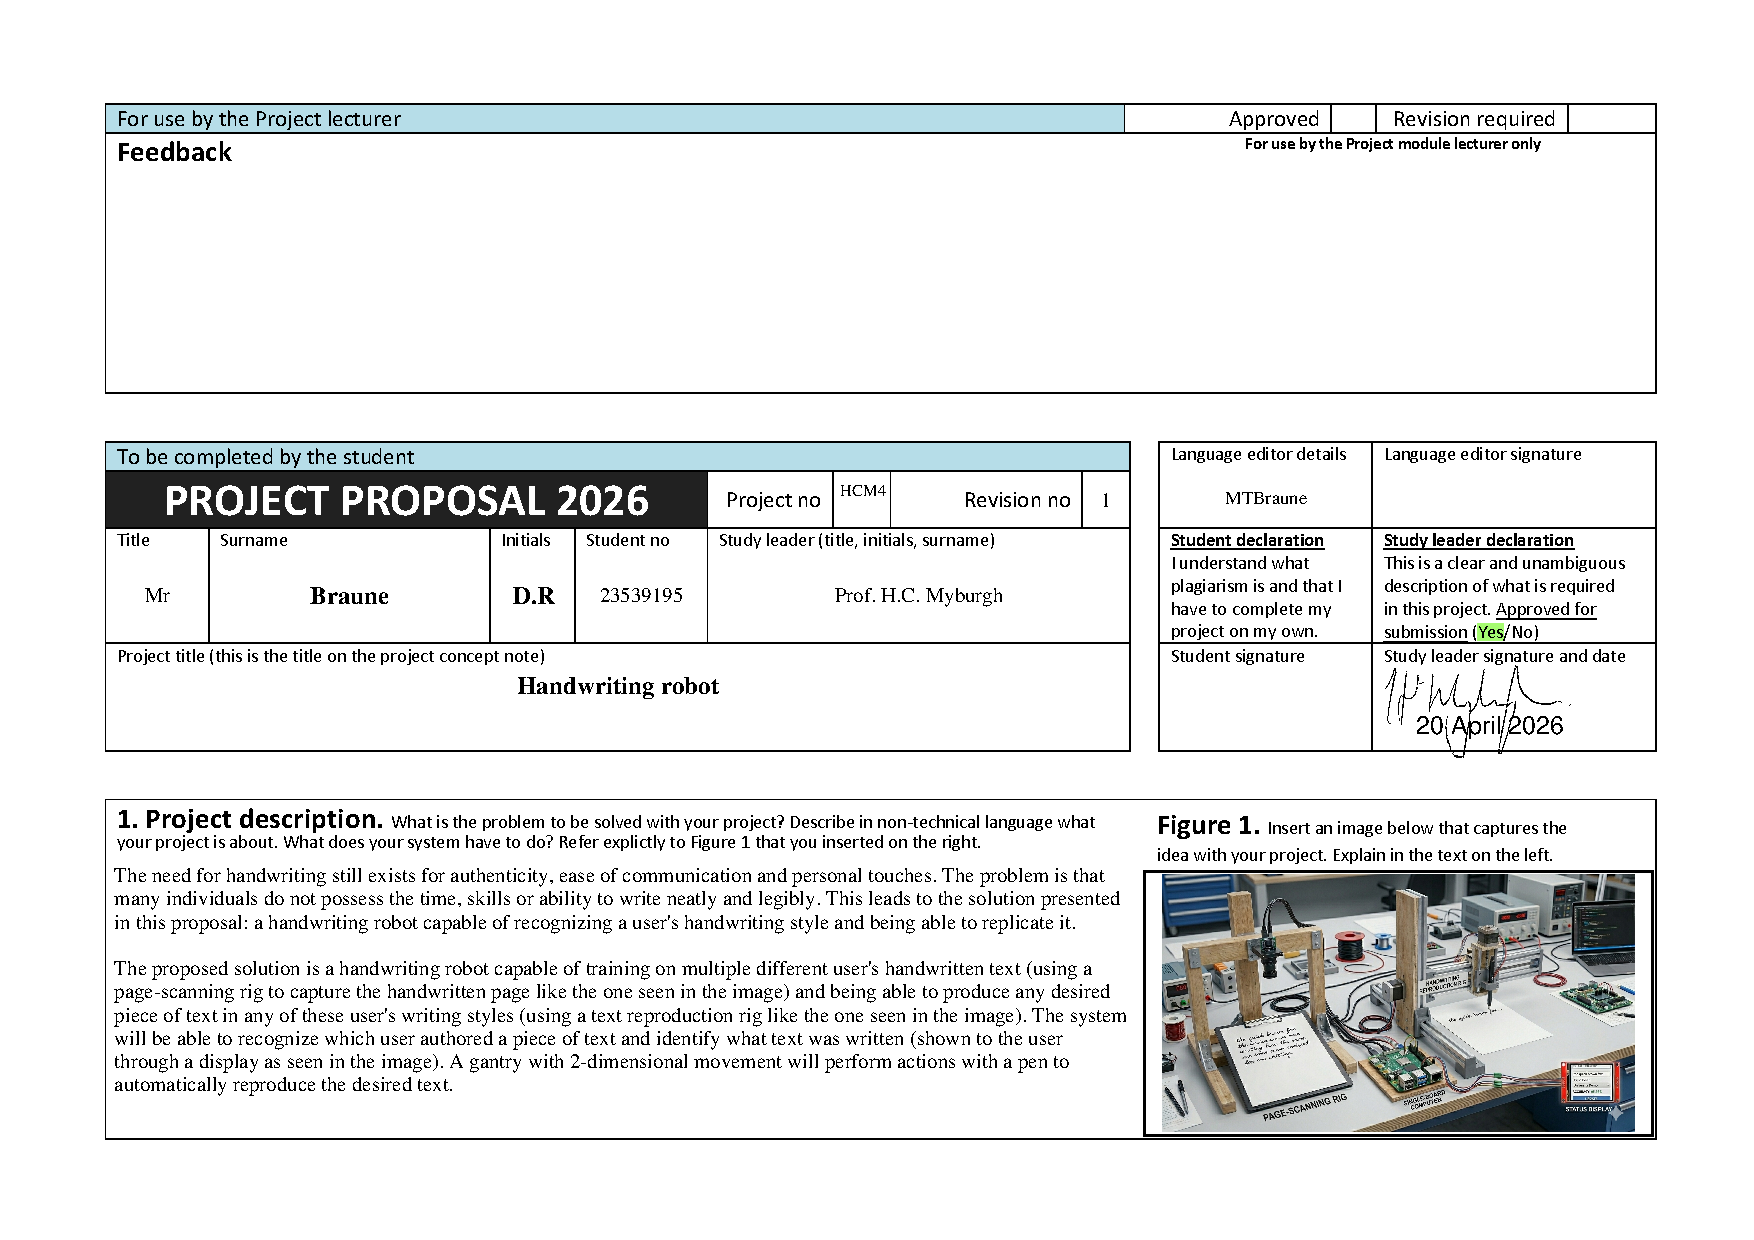
\includepdf[pages=-,landscape]{2_Project_Definition/project_proposal.pdf}


\eprsec{Part 3. Main Report}
\newpage

%% Reset the page number style and count.
\pagenumbering{arabic}
\setcounter{page}{1}

%% Import the main report content

\section{Literature study}
\label{sec:literature}
This section summarises the literature that was required to complete the project and places the work in context; it extends the literature study of the first-semester report. Section~1.1 presents the background as one argument that follows the signal path of the system, from a photograph of a handwritten page, through recognition and writer identification, to the synthesis of new handwriting and its execution by a two-axis robot. Section~1.2 states which technique was adopted for each subsystem, why, and which requirement of the proposal (R1 to R6) it serves.

\subsection{Background and context}
\label{sec:lit-background}

A handwriting-reproduction robot has to solve three problems that are usually studied separately: \emph{reading} (converting an image of handwriting into text), \emph{writer identification} (deciding who wrote it) and \emph{writing} (producing new text in a given person's style and drawing it with a machine). Each topic is treated in turn below, followed by what is known about combining them in one embedded system.

\subsubsection{Handwriting recognition: problem, data and early solutions}
\label{sec:lit-hwr}

Handwriting recognition (HWR) or handwritten text recognition (HTR) converts handwriting into machine-readable text. Plamondon and Srihari~\cite{plamondon2000} distinguish \emph{online} recognition, where the pen position is recorded over time so that stroke order and pen lifts are known, from \emph{offline} recognition, where only an image of the finished writing exists and the time dimension must be inferred. The system in this project reads a photographed page, so it is an offline problem, generally the harder of the two~\cite{plamondon2000}. The distinction also matters for the writing side, because most pen-path generators are trained on online data (Section~\ref{sec:lit-synth}).

The data set fixes the \emph{unit of recognition}. The Extended Modified National Institute of Standards and Technology (EMNIST) data set holds roughly 814\,000 isolated characters of $28\times28$ pixels~\cite{chen2023}; models trained on it classify characters that have already been cut out but cannot read connected writing. The Institute of Computer Science and Applied Mathematics (IAM) database of Marti and Bunke~\cite{marti2002} contains scanned pages of English sentences from many writers (5\,685 sentences, 115\,320 words, 8-bit greyscale at 300 dots per inch) labelled per line, which suits recognisers that read whole lines and also allows writer-related experiments.

Early offline systems followed a \emph{segment-then-classify} paradigm. LeCun \emph{et al.}~\cite{lecun1998} showed that a convolutional neural network (CNN) can classify isolated characters directly from pixels, and their LeNet-5 became the baseline for later character classifiers; many first-semester sources~\cite{chen2023,ji2021,yahya2021,mamun2024} refine such classifiers. For ordinary handwriting their weakness is the segmentation step: in cursive writing letters touch, an incorrect cut yields a fragment that no classifier can label, and the classifier cannot repair the error because it never sees the neighbouring letters. System accuracy is therefore bounded by the accuracy of the segmenter.

\subsubsection{Sequence recognition with neural networks}
\label{sec:lit-nn}

A \emph{convolutional layer} slides a small window of learned weights (a kernel, typically $3\times3$ pixels) over the image and outputs a weighted sum of the pixels under the window followed by a non-linearity; because the weights are shared, a pattern such as a stroke at a given angle is detected wherever it occurs~\cite{lecun1998}. \emph{Max-pooling} keeps the largest value in each small block, halving the resolution, and \emph{batch normalisation}~\cite{ioffe2015} rescales activations to a stable range so that deeper networks can be trained. Weights are learned by minimising a loss: back-propagation gives the gradient of the loss with respect to every weight, and an optimiser such as Adam~\cite{kingma2015} updates the weights against it.

A CNN gives a fixed-size output, whereas a line of text has an unknown number of characters. Recurrent networks process a sequence step by step while carrying a hidden state; the long short-term memory (LSTM) cell~\cite{hochreiter1997} adds gates (input, forget and output) that decide what to store, discard and expose, so that information survives many steps. A \emph{bidirectional} LSTM (BiLSTM) runs one LSTM in each direction so that each position uses the writing on both sides of it, which resolves, for example, a stroke that could be a ``u'' or an ``n''.

The remaining difficulty is the training signal. The network turns a line image into $T$ time steps, but the label is only the transcription, and the alignment between steps and characters is unknown. Connectionist temporal classification (CTC)~\cite{graves2006} solves this. The network outputs at every step a distribution over the characters plus a ``blank'' symbol meaning ``no new character''. A path $\pi$ assigns one symbol to each step, and a collapse function $B$ merges consecutive repeats and then deletes blanks, so that ``--hh-e-ll-ll-o'' becomes ``hello'' (the blank between the two groups of ``l'' allows a genuine double letter). The probability of a target text $Y$ given the image $X$ is the sum over all paths that collapse to it,
\begin{equation}
p(Y\mid X)=\sum_{\pi:\,B(\pi)=Y}\;\prod_{t=1}^{T}p_t(\pi_t\mid X),
\label{eq:lit-ctc}
\end{equation}
where $p_t(\pi_t\mid X)$ is the probability that the network assigns at step $t$ to the symbol $\pi_t$ of the path. The loss is $-\ln p(Y\mid X)$, and although the number of paths is huge, the sum in Equation~\ref{eq:lit-ctc} and its gradient are computed by dynamic programming~\cite{graves2006}. Consequently \emph{no character segmentation and no alignment labels are needed}. At recognition time the best path is approximated by taking the most probable symbol at every step and collapsing it (greedy decoding), or searched with a lexicon or language model. Viterbi's algorithm~\cite{viterbi1967} can also find the most probable alignment between a \emph{known} transcription and the network output (forced alignment), which is used in Section~\ref{sec:lit-synth}.

Graves \emph{et al.}~\cite{graves2009} combined BiLSTM and CTC and reported word accuracies of 74.1\,\% (offline) and 79.7\,\% (online) on IAM-derived data. Shi \emph{et al.}~\cite{shi2017} replaced the raw-pixel input by CNN features, an arrangement named the convolutional recurrent neural network (CRNN): a CNN turns the image into a sequence of feature columns, a bidirectional recurrent network adds context, and CTC supplies the loss. Puigcerver~\cite{puigcerver2017} showed on IAM that a CNN followed by BiLSTM layers matches networks with costlier multidimensional recurrence, and the first-semester sources~\cite{ma2023,kumar2024,hemanth2022} agree that CNN--RNN hybrids combine the CNN's pattern recognition with the RNN's use of context.

\paragraph{Reported accuracies.}\label{sec:lit-acc} Figures are comparable only for the same metric, decoding and split. Quality is expressed as the character error rate (CER), the number of insertions, deletions and substitutions needed to turn the recognised text into the reference (the Levenshtein distance~\cite{levenshtein1966}) divided by the reference length, or as the word error rate (WER); this report uses character accuracy $=1-\text{CER}$. Kizilirmak and Yanikoglu~\cite{kizilirmak2023}, whose CNN--BiLSTM--CTC network is closest to the one used here, report a best CER of 3.59\,\% and WER of 9.44\,\% on IAM, but only with lexicon-constrained decoding and test-time augmentation. Greedy decoding without a lexicon is therefore expected to be worse, and word error rates are several times the character error rate because errors cluster inside words. Accuracies above 95\,\% in the first-semester sources~\cite{yahya2021,ji2021,chen2023} concern isolated characters on clean data, a far easier task. Two further limits apply: benchmark splits may put the same writer, or neighbouring lines of one page, in both training and test partitions, and published work is mostly evaluated on scanner-quality images, whereas an office photograph has uneven lighting, perspective, shadows and neighbouring objects. This gap is why pre-processing cannot be omitted.

\subsubsection{Image pre-processing and page segmentation}
\label{sec:lit-prep}

Before a recogniser can read a photographed page, the page must be converted to clean, separated line images; the first-semester sources~\cite{chen2023,hemanth2022} list normalisation, binarisation and line separation by bounding boxes around ink regions as the standard steps.

A photograph records the product of the paper's reflectance and the lighting, so a lamp gradient or shadow changes the grey value of the paper itself. \emph{Binarisation} decides for each pixel whether it is ink or paper. Otsu's global method~\cite{otsu1979} picks the threshold $t^{*}$ that maximises the between-class variance of the two groups of pixels,
\begin{equation}
t^{*}=\arg\max_{t}\;\omega_{B}(t)\,\omega_{F}(t)\,\bigl[\mu_{B}(t)-\mu_{F}(t)\bigr]^{2},
\label{eq:lit-otsu}
\end{equation}
where $\omega_B(t)$ and $\omega_F(t)$ are the fractions of pixels at or below, and above, the candidate $t$, and $\mu_B(t)$ and $\mu_F(t)$ are their mean grey values. It needs no tuning but fails under uneven lighting, because one threshold then drops strokes in dim areas or turns shadows into ink. \emph{Adaptive} methods use a threshold per pixel: Sauvola and Pietik\"ainen~\cite{sauvola2000} derive it from the local mean and standard deviation, and Bradley and Roth~\cite{bradley2007} compare each pixel with the local mean computed from an integral image. Dividing the image by a heavily blurred copy of itself (flat-field correction) turns a multiplicative lighting gradient into a nearly constant white paper level. Local means over large windows are made cheap by the summed-area table of Crow~\cite{crow1984}, which stores at each position the sum of all pixels above and to the left, so that the sum over any rectangle needs only four look-ups regardless of its size; three repeated box averages also approximate a Gaussian blur.

Ink pixels are grouped into \emph{connected components} by the two-pass labelling of Rosenfeld and Pfaltz~\cite{rosenfeld1966}. Component heights give a typical character height that can serve as a scale reference, so that thresholds expressed in character heights do not depend on camera resolution or handwriting size. A tilted page is corrected by a projection-profile search: the image is rotated through trial angles and the angle at which the row-wise ink histogram is most sharply peaked is taken as the skew. Lines are formed either from gaps in the row profile, which assumes straight horizontal lines, or by chaining neighbouring components from left to right, which tolerates drifting baselines and diagrams. Printed ruling lines glue letters together and must be removed without deleting the pen strokes that cross them. These steps are mature but mostly described for scanned documents, rarely for a camera, a desk background, ruled paper and diagrams together.

\subsubsection{Writer identification and style}
\label{sec:lit-writer}

Writer identification asks which member of a known set wrote a sample. The proposal grounded its target in signature classification: Agduk and Aydemir~\cite{agduk2022} compared transfer-learning CNNs for classifying signatures by person and gender. Signatures are short and practised, but they are not free text, whereas this system must identify the writer of running text while also reading it. The statistical approach of Bulacu and Schomaker~\cite{bulacu2007} is \emph{text independent}: it compares histograms of contour direction and curvature (texture level) and of characteristic letter shapes (allograph level). Style can also be described by slant, x-height (the height of the lower-case body), stroke width, spacing and the frequency of joined letters. The learning approach trains a CNN directly on handwriting images; He and Schomaker's FragNet~\cite{he2020} classifies small fragments and pools the evidence, exploiting the fact that style is present in every part of a text.

Two cautions affect the project. A classifier trained on real ink can rely on cues that a machine cannot reproduce: stroke thickness and ink density depend on the writer's pen pressure and pen, whereas a robot draws with one pen at a constant width. And most of this work uses hundreds of writers, whereas a closed set of ten writers with about one thousand text lines is much smaller, and test partitions that share pages with training data inflate accuracy in such small experiments.

\subsubsection{Handwriting synthesis and pen-path generation}
\label{sec:lit-synth}

\emph{Neural sequence generators} are trained on recorded pen trajectories. Graves~\cite{graves2013} used an LSTM conditioned on the text through a soft attention window, whose output at each step is a mixture density over the next pen offset and a pen-up probability; it produces convincing cursive but needs pen recordings of the writer, generally hundreds to thousands of lines, which photographs of a few pages cannot supply. Image generators such as the generative adversarial network of Kang \emph{et al.}~\cite{kang2020} need less data per writer after pre-training on a large corpus, but they produce raster images that must still be converted to pen paths and give no direct control of slant, size or spacing. \emph{Exemplar} (glyph-based) methods are the alternative: Haines \emph{et al.}~\cite{haines2016} synthesise text in an author's hand from an annotated sample by assembling extracted glyphs with learned spacing, thickness and pressure. They need only a few pages per writer, have interpretable parameters and stay faithful to the real letterforms. Glyphs can be extracted without hand-drawn boundaries by forced alignment of the known transcription with the output of a trained recogniser (Section~\ref{sec:lit-nn}).

Turning a glyph into a pen path needs classical steps. \emph{Thinning} reduces a stroke to a one-pixel centre line without breaking connectivity; the parallel algorithm of Zhang and Suen~\cite{zhang1984} deletes boundary pixels in two alternating sub-iterations according to the pattern of their eight neighbours. The centre line is traced into ordered point sequences, which the Douglas--Peucker algorithm~\cite{douglas1973} simplifies by keeping the end points and recursively keeping the point farthest from the chord whenever its distance exceeds a tolerance $\varepsilon$; the first-semester report noted that it is not guaranteed to be optimal.

\subsubsection{Robotic writing and linear motion}
\label{sec:lit-robot}

The first-semester study identified three robot topologies~\cite{teikari2016}. A \emph{Cartesian} (gantry) system moves along two perpendicular linear axes: it is mechanically simple, its kinematics are the identity and it covers a flat page naturally. \emph{Serial-chain} arms reach a larger volume but need inverse kinematics and joint errors add up at the pen. \emph{Parallel} robots are stiff and precise but have a small workspace and complex kinematics. Belt-drive, rack-and-pinion and ball-screw actuators have been used in handwriting systems for their durability, reliability and low cost~\cite{iqs2024}.

Most such systems use stepper motors, which turn by a fixed angle for every pulse. A driver converts a logic-level pulse (STEP) and direction level (DIR) into winding currents, and microstepping gives finer positions; Acarnley~\cite{acarnley2002} treats open-loop stepping, torque--speed limits and the use of controlled acceleration (for example a trapezoidal velocity profile) to avoid lost steps. Because position follows from counting pulses, error does not accumulate if commanded positions are converted to integer step counts from a known reference. To draw a straight line with two independent axes the pulses must be interleaved; Bresenham's algorithm~\cite{bresenham1965}, developed for digital plotters, does this in integer arithmetic: the faster axis steps every cycle and an error accumulator decides when the slower axis also steps, so the deviation from the ideal line never exceeds one step.

Published robots show what accuracy to expect. The proposal used Teikari's analysis~\cite{teikari2016} to set about four seconds per character for between zero and one per cent error, the 0.3\,mm absolute gantry error reported by Huang and Xiong~\cite{huang2024} as the basis of the 0.5\,mm limit of R5, and the roughly 85\,\% accuracy derived from Babushkin \emph{et al.}~\cite{babushkin2025} for acceptable character accuracy (R1). None of these shows how a robot would reproduce an \emph{identified} person's style from a photograph of that person's page.

\subsubsection{Embedded deployment and shortcomings of the literature}
\label{sec:lit-embedded}

Executing all processing on a single-board computer (SBC) raises the cost of every algorithm above. Sze \emph{et al.}~\cite{sze2017} stress that multiply--accumulate operations and the memory for weights and activations determine execution time and energy on a constrained processor, and that convolutions usually dominate. A line recogniser with a convolutional front end costs of the order of $10^{9}$ operations per image, whereas the classical image-processing steps need only a few operations per pixel, especially with integral images. The first-semester report observed that most research also relies on large off-the-shelf frameworks, so that the algorithms themselves are never exposed~\cite{chen2023}.

Four shortcomings follow. First, recognition, writer identification, synthesis and robotics are studied in isolation, with no complete system from a photographed page to a drawn page. Second, embedded deployment is rarely demonstrated, and then usually through frameworks. Third, reported accuracies depend on benchmark conditions (lexicon, scanner images, shared writers or pages) that differ from a photographed page. Fourth, the generation literature needs recorded pen trajectories or large pre-training and evaluates output as an image, whereas this project must evaluate output that a machine can draw with a constant-width pen. These define the contribution of the project.

\subsection{Application of the background to this project}
\label{sec:lit-application}

This section records how each subsystem applied what was learnt; the detailed designs follow in Section~3.

\subsubsection{Reading and identification (R2, R4)}

Cursive writing cannot be segmented reliably, a segmentation error cannot be repaired by the classifier, and the labels are line transcriptions, so a line-level recogniser trained with CTC~\cite{graves2006} was adopted and FU\,2.2 (character separation) was realised as separation into \emph{lines}. The architecture follows the CNN--BiLSTM--CTC pattern~\cite{shi2017,puigcerver2017,kizilirmak2023}: a fixed $64\times640$ input (lower than the $100\times960$ of the published network, to make training practicable), twelve convolutional layers with batch normalisation, two max-pooling layers, two BiLSTM layers and a linear output over 74 characters plus the blank, with about 3.36 million parameters. Decoding is greedy, because lexicon decoding needs additional corpora and the published lexicon figures cannot be assumed to transfer. At the design stage the recogniser reached 94.03\,\% and 91.82\,\% character accuracy on the validation and test partitions of a public line data set (the validation figure also selected the final checkpoint, so only the test figure is free of selection), and 89.4\,\% character and 70.8\,\% word accuracy on lines of the ten writers not used for training; for the two personal writers these lines came from the same pages as the training lines, and for the eight public-data writers independence from the larger training corpus is not fully verified. These character accuracies lie below the 95\,\% overall figure of R2, which is therefore evaluated explicitly in Section~4 and not assumed to be met.

Because benchmark conditions rarely reflect a photographed page, the pre-processing chain was written from first principles from the techniques of Section~\ref{sec:lit-prep}: rescaling and division by a blurred background estimate; a local mean threshold with a fixed offset evaluated with summed-area tables, so that its cost is independent of window size; a projection-profile skew search; run-length two-pass component labelling; and chaining of components into lines with thresholds that are multiples of the estimated character height. Otsu's threshold~\cite{otsu1979} was retained for locating the sheet against the desk and for clean line crops. The Sauvola method~\cite{sauvola2000} was not adopted, because its standard-deviation term needs a second integral image and the offset-based local mean sufficed for the photographs used; perspective correction was omitted because the camera looks straight down at the page.

For writer identification a learned CNN on text lines was chosen over hand-crafted statistics~\cite{bulacu2007} or fragment pooling~\cite{he2020}, because the recogniser's convolutional features could be reused and accuracy could be measured directly. Following the caution of Section~\ref{sec:lit-writer}, two classifiers with the same architecture (966\,154 parameters) were built. The first sees the unmodified ink of real photographs and classifies a page by averaging per-line probabilities. The second sees lines thinned to a centre line and redrawn at a constant width proportional to the x-height, which removes thickness and pressure cues and matches what the gantry can do; only its final 13\,354 classification-head parameters were trained, on top of the recogniser's frozen features. The first was almost perfect on real handwriting but about 20\,\% accurate on synthesised output, which motivated the second. Both are closed-set decisions among ten writers; they address R2 and the ten-style storage of R6 but cannot report an unknown writer.

\subsubsection{Reproduction (R1, R3, R5, R6)}

Neural trajectory generators need pen recordings that the project does not have, and image generators lack parametric control and produce rasters, so an exemplar approach in the manner of Haines \emph{et al.}~\cite{haines2016} was adopted. For each of ten writers, glyphs are harvested from about nine scanned pages: the recogniser aligns the known transcription with the line, the ink is cut into letter territories, thinned~\cite{zhang1984}, traced into strokes, simplified~\cite{douglas1973} (tolerance 0.6 pixels), normalised to the x-height and de-slanted. The glyphs and measured style statistics form a \emph{style profile} stored permanently as a data file, which realises FU\,2.5 to 2.7. Synthesis chooses glyphs, shears them to the writer's slant, spaces them with the writer's statistics and adds small random variation; because each run is random, several candidates are generated and the one with the best combined score of recogniser legibility and writer-classifier confidence is kept. In design-stage experiments, selection among fourteen candidates raised the writer-identification rate of the synthetic output from 79.2\,\% to 97.5\,\% and the character accuracy from 75.9\,\% to 81.6\,\%. These figures must be read with caution: the judging networks also perform the selection, so the result is not an independent verdict, no human assessment was carried out, and the character accuracy remains below the 85\,\% target of R1. Section~4 presents the evaluation against R1.

A Cartesian gantry with stepper motors was adopted, since position follows from step counts, the only practical route to 0.5\,mm without position sensors. Pen paths in millimetres are converted to G-code (a standard line-oriented machine instruction language) and executed by a program that converts coordinates to absolute integer step counts, interleaves the axes with Bresenham's algorithm~\cite{bresenham1965} and reads the limit switches before every step. For the nominal mechanics (sixteen microsteps per full step and a belt advance of 40\,mm per revolution, to be confirmed) one step is 12.5\,$\mu$m, eighty times finer than the 0.5\,mm limit of R5. The trapezoidal profile is used only in the drawing-time estimate; executed motion runs each segment at constant feed, and whether ramps are needed was not investigated. Resolution is not accuracy: belt stretch, backlash, home-switch repeatability and pen compliance determine the true error. \textbf{[TO BE COMPLETED BY STUDENT: confirm the motor, driver, microstepping and belt/pulley specification of the built gantry, and state the measured positional error against the 0.5\,mm limit of R5, if measured.]}

\subsubsection{Embedded execution and the contribution}

Following Sze \emph{et al.}~\cite{sze2017}, the cost of the networks was analysed in operations and memory: about $4.2\times10^{9}$ multiply--accumulate operations and 13.4\,MB of weights per recogniser pass over a line, 91\,\% of the arithmetic being convolution. Inference of both networks was therefore written from first principles in the Python language as matrix multiplications (each convolution rearranged into one large product) and element-wise operations, without a neural-network framework; it agrees with the training implementation to about $10^{-5}$ in log-probability on a test input. A recogniser pass took 2.6 to 3.1\,s per line on the development computer; no timing on the target SBC was found, so the 25\,ms per character plus 2\,s of R4 cannot yet be assessed. \textbf{[TO BE COMPLETED BY STUDENT: measured inference and segmentation times on the ODROID N2+ for a typical page.]} The contribution that follows from the shortcomings of Section~\ref{sec:lit-embedded} is a complete pipeline from page photograph to pen strokes, implemented from first principles in one language.

\newpage

\section{Approach}
\label{sec:approach}
This section explains how the problem of the approved proposal was approached, before the technical detail of Section~3. It answers \emph{how} the functional analysis was translated into a first concept and which alternatives were weighed for each major decision, and \emph{why} the subsections of Section~3 appear in their order and which requirement each serves. The description is conceptual; mathematics and parameter values are deferred to Section~3.

\subsection{From functional analysis to concept}
\label{sec:app-concept}

The proposal defined three modes (training, classification and reproduction) and four functional units: FU\,1, the page-scanning setup; FU\,2, the single-board computer (SBC) with blocks 2.1 image conditioning, 2.2 character separation, 2.3 classification, 2.4 back-propagation, 2.5 conversion of characters to trajectory maps, 2.6 permanent storage, 2.7 loading and 2.8 stepper-pulse generation; FU\,3, the gantry (3.1 voltage shifter, 3.2 X/Y motor control, 3.3 pen and paper adjustment, 3.4 pen movement control); and FU\,4, the power supply. Requirements R1 to R6 and two field conditions, FC1 (a well-lit room, 400 to 1000\,lux) and FC2 (a stable, level, vibration-free surface), were attached to this structure.

The first concept kept the structure and made one decision per block. A fixed camera above the page provides FU\,1. The SBC conditions the image, separates the page into units that a classifier can read, reads the text, identifies the writer and, in training mode, builds a permanent library of the writer's letter shapes. The gantry receives only step and direction pulses. Figure~\ref{fig:app-concept} shows the concept with its three modes, and Table~\ref{tab:app-fu} states how each unit was realised and where it departs from the proposal; the departures are justified in Section~\ref{sec:app-alternatives}.

\begin{figure}[htbp]
\centering
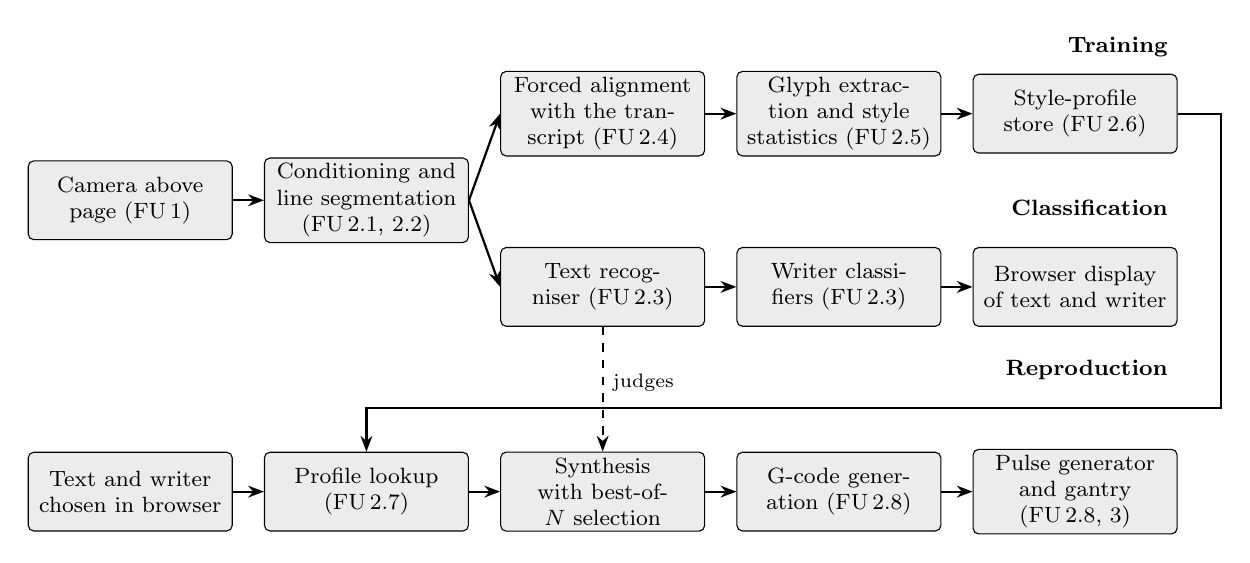
\begin{tikzpicture}[
  blk/.style={draw,rounded corners=2pt,fill=gray!15,minimum height=1.0cm,text width=2.45cm,align=center,font=\footnotesize,inner sep=2pt},
  arr/.style={-{Stealth[length=2mm]},thick},
  darr/.style={-{Stealth[length=2mm]},thick,dashed},
  lab/.style={font=\footnotesize\bfseries,anchor=east}]
\node[blk] (cam) at (0,-1.1) {Camera above page (FU\,1)};
\node[blk] (seg) at (3,-1.1) {Conditioning and line segmentation (FU\,2.1, 2.2)};
\node[blk] (ali) at (6,0) {Forced alignment with the transcript (FU\,2.4)};
\node[blk] (gly) at (9,0) {Glyph extraction and style statistics (FU\,2.5)};
\node[blk] (sto) at (12,0) {Style-profile store (FU\,2.6)};
\node[blk] (rec) at (6,-2.2) {Text recogniser (FU\,2.3)};
\node[blk] (wid) at (9,-2.2) {Writer classifiers (FU\,2.3)};
\node[blk] (dis) at (12,-2.2) {Browser display of text and writer};
\node[blk] (inp) at (0,-4.8) {Text and writer chosen in browser};
\node[blk] (lkp) at (3,-4.8) {Profile lookup (FU\,2.7)};
\node[blk] (syn) at (6,-4.8) {Synthesis with best-of-$N$ selection};
\node[blk] (gco) at (9,-4.8) {G-code generation (FU\,2.8)};
\node[blk] (gan) at (12,-4.8) {Pulse generator and gantry (FU\,2.8, 3)};
\draw[arr] (cam)--(seg);
\draw[arr] (seg.east)--(ali.west);
\draw[arr] (ali)--(gly); \draw[arr] (gly)--(sto);
\draw[arr] (seg.east)--(rec.west);
\draw[arr] (rec)--(wid); \draw[arr] (wid)--(dis);
\draw[arr] (inp)--(lkp); \draw[arr] (lkp)--(syn); \draw[arr] (syn)--(gco); \draw[arr] (gco)--(gan);
\draw[arr] (sto.east) -- ++(0.55,0) |- ($(lkp.north)+(0,0.55)$) -- (lkp.north);
\draw[darr] (rec.south) -- node[right,font=\scriptsize,pos=0.45]{judges} (syn.north);
\node[lab] at (13.3,0.85) {Training};
\node[lab] at (13.3,-1.2) {Classification};
\node[lab] at (13.3,-3.25) {Reproduction};
\end{tikzpicture}
\caption{Block diagram of the chosen concept. Solid arrows show the flow of data; the dashed arrow shows that the recogniser and writer classifier also judge the candidates in the synthesis block. Functional-unit numbers of the proposal are in brackets. Training is performed offline and is not part of the browser interface.}
\label{fig:app-concept}
\end{figure}

\begin{table}[htbp]
\centering
\fontsize{9}{10.5}\selectfont
\begin{tabularx}{\linewidth}{|p{1.5cm}|X|X|}
\hline
\textbf{Unit} & \textbf{Realisation in the final concept} & \textbf{Departure from the proposal} \\
\hline
FU\,1, 2.1 & Camera on a fixed rig over an A4 page; conditioning of the photograph (scale, lighting, binarisation, skew, ruled lines). & None; conditioning is far more extensive than anticipated. \\
\hline
FU\,2.2 & Separation of the page into \emph{text lines}. & Lines instead of characters (Section~\ref{sec:app-alternatives}). \\
\hline
FU\,2.3, 2.4 & Line recogniser for text, two classifiers for the writer; gradient-based training offline. & Text and writer by separate networks; training not in the interface. \textbf{[TO BE COMPLETED BY STUDENT: state on which computer the networks were trained and the profiles built; the proposal requires embedded-only processing.]} \\
\hline
FU\,2.5--2.7 & A style profile per writer (pen-path glyphs and style statistics) stored permanently as a data file and loaded at start-up. & Stored per glyph variant with statistics, not one map per character. \\
\hline
FU\,2.8, 3.1, 3.2 & G-code, then step/direction pulses generated by the SBC for two stepper-driver modules; limit switches bound the travel. & Two stages; limit switches added as a safety function. \\
\hline
FU\,3.3, 3.4 & Pen and paper holders; pen lifted by a one-way toggle gear motor with a position switch. & Pen lift not controlled through the stepper driver. \textbf{[TO BE COMPLETED BY STUDENT: reason for this change.]} \\
\hline
FU\,4 & Power supply. & \textbf{[TO BE COMPLETED BY STUDENT: supply voltages, current ratings and distribution.]} \\
\hline
\end{tabularx}
\caption{Translation of the functional units of the proposal into the first concept.}
\label{tab:app-fu}
\end{table}

\subsection{Design alternatives and trade-offs}
\label{sec:app-alternatives}

For each major decision the options offered by the literature of Section~1 and the proposal were compared against criteria derived from the requirements: accuracy (R1, R2), processing time on the SBC (R3, R4), the data available for ten writers (R6), the need for first-principles implementation, and mechanical and electrical simplicity and safety. The comparisons are mostly qualitative arguments; where design-stage measurements supported a decision they are quoted with their caveats. Table~\ref{tab:app-software} covers the processing chain and Table~\ref{tab:app-hardware} the physical system.

\begin{table}[htbp]
\centering
\fontsize{9}{10.5}\selectfont
\begin{tabular}{|p{1.6cm}|p{3.4cm}|p{4.3cm}|p{4.3cm}|}
\hline
\textbf{Decision} & \textbf{Alternatives} & \textbf{Comparison} & \textbf{Preferred and reason} \\
\hline
Unit of recognition & (a) Cut characters, classify each. (b) Cut lines, read with a sequence recogniser. & (a) Needs a segmenter that works on joined letters and character-level labels (absent); cannot repair a wrong cut. (b) No boundaries below the line; uses context; larger network. & (b): cursive cannot be segmented reliably, labels exist per line, and segmenter errors would bound system accuracy. \\
\hline
Networks for text and writer & (a) One network, two outputs. (b) Separate networks. & (a) One computation, but the tasks compete. (b) Each trainable and measurable alone. & (b): an early joint network learned the writer quickly while text accuracy stayed very low (training-script documentation; log not kept). \\
\hline
Synthesis of writing & (a) Neural generator on pen trajectories. (b) Pretrained image generators. (c) Library of the writer's own glyphs. & (a) Needs recorded pen trajectories (unavailable). (b) Raster output, no control of size or slant, slow without a graphics processor. (c) About nine pages per writer, strokes with controllable parameters; cursive links partly lost. & (c): a from-scratch generator trained on stroke data from the photographs learned slant and roundness but not legible letters; image generators took tens of seconds per line on a processor-only computer. \\
\hline
Selection of output & (a) Use the first result. (b) Draw $N$ candidates, keep the best by recogniser and writer classifier jointly. & (a) Fastest, but random variation gives good and bad results. (b) Time grows with $N$. & (b): with $N=14$ writer identification of the synthetic output rose from 79.2\,\% to 97.5\,\% and character accuracy from 75.9\,\% to 81.6\,\%; the judges also select, so this is not independent evidence. \\
\hline
Location of processing & (a) Offload to a personal computer. (b) All inference on the SBC. & (a) Faster, but contradicts the proposal. (b) Limits memory, compute and methods. & (b), as required; method cost was considered throughout (Section~\ref{sec:lit-embedded}). \\
\hline
\end{tabular}
\caption{Software design decisions, alternatives and reasons for the preferred solution.}
\label{tab:app-software}
\end{table}

\begin{table}[htbp]
\centering
\fontsize{9}{10.5}\selectfont
\begin{tabular}{|p{1.6cm}|p{3.4cm}|p{4.3cm}|p{4.3cm}|}
\hline
\textbf{Decision} & \textbf{Alternatives} & \textbf{Comparison} & \textbf{Preferred and reason} \\
\hline
Page capture & (a) Fixed camera. (b) Flatbed scanner. & (a) Instant capture, standard interface, live framing; lighting and tilt handled in software (FC1 applies). (b) Even lighting; larger separate device with a scanning delay. & (a): suits the compact rig and the capture budget of R4; cost is the extensive conditioning of Section~\ref{sec:segmentation}. \\
\hline
Robot type & (a) Cartesian gantry. (b) Serial arm. (c) Parallel robot. & (a) Identity kinematics, flat page, axis errors do not add up. (b) Inverse kinematics, joint errors add up. (c) Stiff, but small workspace, complex kinematics. & (a): position follows from step counts; the 0.5\,mm limit of R5 is simplest to meet and verify~\cite{teikari2016}. \\
\hline
Motor control & (a) Separate microcontroller receives moves. (b) SBC generates STEP/DIR pulses. & (a) Offloads timing, but an issued move cannot be stopped without a round trip. (b) Less deterministic timing; limit switches read before every step. & (b): stopping within one step on a limit-switch trip was valued above deterministic timing. \\
\hline
\end{tabular}
\caption{Hardware design decisions, alternatives and reasons for the preferred solution.}
\label{tab:app-hardware}
\end{table}

Two consequences deserve emphasis. Rejecting segmentation below the line means the recogniser is trained from line transcriptions with connectionist temporal classification~\cite{graves2006}, at the price of a larger network and a heavier dependence on robust \emph{line} segmentation. The glyph library gives up the natural variation of a neural generator for control and a small data requirement; heavily cursive hands, whose letter links are lost when letters are cut apart, were recognised from the outset as its weak case.

\subsection{Off-the-shelf components and own design}
\label{sec:app-offshelf}

Consistent with rows 5 and 6 of the requirement tables of the proposal, the following were taken off the shelf: the camera and its driver, the SBC (an ODROID N2+), the stepper motors and driver modules, the limit switches, the pen, standard gantry parts (belts or screws, bearings, fasteners), storage and the power supply. Camera and general-purpose input/output access use standard system drivers for hardware interfacing only. The student designed and implemented the image conditioning and page segmentation; the recogniser and writer classifiers with their training; the style-profile builder, synthesiser and candidate selection; the conversion of pen paths to G-code and of G-code to step pulses with safety checks; the gantry calibration; the browser interface; and the mechanical parts designed in computer-aided design software for the gantry. \textbf{[TO BE COMPLETED BY STUDENT: list of the mechanical parts designed and manufactured, as opposed to purchased.]}

\subsection{Verification strategy and roadmap}
\label{sec:app-verification}

The design was verified against two kinds of evidence. The first is performance on data \emph{held out} from training: a public line-level partition for the recogniser, and one whole page per public-data writer for the writer classifiers. The partition for the two personal writers is weaker, since held-out lines come from the training pages, and this is stated wherever the figures are quoted. The second is the proposal's \emph{measurable specifications}: character and style accuracy (R1), text and writer accuracy (R2), time per character (R3, R4), absolute positional error (R5) and number of stored styles (R6); Section~4 reports what was and was not measured. Two limitations were recognised at the outset: synthesis was both tuned and judged with the same two networks, so its figures measure agreement with these judges, and the recogniser's accuracy on real handwriting of the same writers is the non-circular reference; and the figures for R3, R4 and R5 depend on the built hardware and the SBC and can only be obtained by timing and positional measurements on the built system.

Section~3 follows the path of the data, because each stage uses the output of the preceding one. After the overall architecture (Section~\ref{sec:blockdiagram}), page conditioning and line segmentation (Section~\ref{sec:segmentation}) come first, since every later stage needs clean line images and FC1 and FC2 act here (R2, R4). The text recogniser (Section~\ref{sec:textrec}; R2, R4) precedes the writer classifier (Section~\ref{sec:writerid}; R2, R6), which starts from its features. The style profile (Section~\ref{sec:styleprofile}) is built from the segmented lines with the trained recogniser and is followed by synthesis and candidate selection (Section~\ref{sec:synthesis}); both serve R1 and the profile also R6. G-code generation (Section~\ref{sec:gcode}) and the gantry with its control (Section~\ref{sec:gantry}) form the final physical stage (R3, R5), and integration into one system, with its interface and timing chains (Section~\ref{sec:system}), closes the section (R3, R4). R1 is the most important requirement but is addressed after the networks because it rests on everything upstream.

\newpage

\section{Design and implementation}
% ---- Writer 2 shared definitions (used by 3.1 - 3.5) ----
\providecommand{\wht}{h_{\mathrm{t}}}
\tikzset{
  w2box/.style={draw,rounded corners=2pt,fill=gray!12,align=center,font=\footnotesize,minimum height=7mm,inner sep=3pt},
  w2dark/.style={draw,rounded corners=2pt,fill=gray!30,align=center,font=\footnotesize,minimum height=7mm,inner sep=3pt},
  w2store/.style={draw,fill=white,align=center,font=\footnotesize,minimum height=7mm,inner sep=3pt,double,double distance=1pt},
  w2io/.style={draw,rounded corners=6pt,fill=white,align=center,font=\footnotesize,minimum height=7mm,inner sep=3pt},
  w2arr/.style={-{Stealth[length=2.2mm]},thick},
  w2dash/.style={-{Stealth[length=2.2mm]},thick,dashed},
  w2group/.style={draw,dashed,rounded corners=4pt,inner sep=5pt},
  w2lab/.style={font=\scriptsize,inner sep=1.5pt}
}

\subsection{Design summary}
\label{sec:summary}

This section summarises the project design tasks and how they were implemented (see Table~\ref{tab:des-summary}).
The rows follow the deliverables of line~5 of the table of Section~4 of the approved project proposal (requirements R1 to R6, ``own design contribution'') and the design and implementation tasks of Section~6.1 of that proposal.
R1 is reproduction of text in the style of any writer of the training set, R2 decoding of the text and identification of the writer, R3 reproduction speed, R4 classification time, R5 gantry positional accuracy and R6 at least ten stored writing styles.
Only work designed and implemented by the student is claimed; the physical parts that were bought as finished items (camera, single-board computer, stepper motors and driver modules, pen, end-stop switches, power supply, standard mechanical parts) carry no design credit.
All image-processing, machine-learning, trajectory and motion-control algorithms were written by the student in Python, and the only external functions used interface with the camera, the file system and the network.

Two deviations from the proposal shape several rows.
First, the proposal planned an explicit separation of the page into characters (functional unit (FU) 2.2) before classification; the implemented design separates the page into \emph{text lines} only and reads each line with a sequence recogniser, because the characters of connected handwriting have no reliable boundaries and a segmentation error would pass directly into a wrong reading (Sections~\ref{sec:segmentation} and~\ref{sec:textrec}).
Second, the proposal placed training and the building of trajectory maps on the single-board computer (FU 2.4 to 2.6); in the implemented system the networks and the per-writer style profiles are produced by offline programs on a general-purpose computer, and only inference, synthesis and motion control run on the single-board computer, so the training mode is not offered by the user interface.
\textbf{[TO BE COMPLETED BY STUDENT: state the computer used for network training (the project notes mention a laptop processor and a cloud notebook) and confirm that the single-board computer was not used for training.]}

{
\fontsize{9.5}{11.5}\selectfont
\setlength{\tabcolsep}{4pt}
\renewcommand{\arraystretch}{1.05}
\begin{longtable}{|p{3.3cm}|p{7.0cm}|p{4.3cm}|}
\hline
\textbf{Deliverable or task} & \textbf{Implementation} & \textbf{Completion of deliverable or task, and section in the report} \\
\hline
\endfirsthead
\hline
\textbf{Deliverable or task} & \textbf{Implementation} & \textbf{Completion of deliverable or task, and section in the report} \\
\hline
\endhead
\hline
\multicolumn{3}{r}{\emph{continued on the next page}}\\
\endfoot
\hline
\endlastfoot
Image conditioning and noise removal (FU 2.1; R2, R4) &
Designed and implemented from first principles using only array arithmetic: size normalisation, page localisation, flat-field illumination correction with summed-area tables, local adaptive thresholding, skew correction and removal of printed rules, faint print and neighbouring-page ink. &
Completed. Section~\ref{sec:segmentation}. Processing time on the single-board computer: \textbf{[TO BE COMPLETED BY STUDENT]}. \\
\hline
Separation into characters (FU 2.2; R2, R4) &
Replaced by separation into text lines and diagram regions (connected components, glyph-scale estimation, chaining, baseline merging, text versus non-text scoring, one deskewed crop per line). Character territories are derived only offline, by forced alignment, when style profiles are built (Section~\ref{sec:styleprofile}). &
Completed as modified (lines instead of characters). Sections~\ref{sec:segmentation}, \ref{sec:textrec}. \\
\hline
Neural network that decodes the text (FU 2.3; R2) &
Convolutional and bidirectional recurrent network with connectionist temporal classification (CTC) output, 3\,358\,763 trainable parameters. The layer pattern follows a published design \cite{kizilirmak2023}; the student chose the input geometry, data pipeline, label cleaning, augmentation and staged joint training, wrote the training code and a separate from-scratch inference implementation. &
Completed. Section~\ref{sec:textrec}; accuracy in Section~\ref{sec:results}. \\
\hline
Neural network that identifies the writer (FU 2.3; R2) &
Two ten-class convolutional classifiers: an ink-based one for photographs and one whose input is re-drawn at a constant pen width (stroke normalisation by thinning and re-inking, designed by the student), with page-level aggregation. &
Completed. Section~\ref{sec:writerid}. \\
\hline
Training on datasets and choice of layer numbers (FU 2.4; simulation on existing datasets) &
Training programs for the recogniser (four stages) and both classifiers on a public database, a public line-level set and 13 photographed personal pages. A sweep over widths, depths and learning rates was programmed but no result was kept, so the layer numbers are those of the published design. Training is offline. &
Completed for training and data pipeline; \textbf{incomplete} for the architecture sweep. Sections~\ref{sec:textrec}, \ref{sec:writerid}. \\
\hline
Capture rig and deployment on the single-board computer (FU 1; R2, R4) &
A generic USB camera is read with a live preview and a five-frame warm-up; recognition, synthesis and motion programs run on the ODROID N2+ behind a web server. Rig geometry, camera resolution and lighting: \textbf{[TO BE COMPLETED BY STUDENT: camera model, resolution, mounting height, field of view, lamp, lux readings, photograph.]} &
Software completed; hardware description \textbf{to be completed}. Sections~\ref{sec:blockdiagram}, \ref{sec:system}. \\
\hline
Trajectory maps and permanent storage (FU 2.5 to 2.7; R1, R6) &
Letter shapes are harvested by forced alignment with the recogniser, thinned to centre-line pen paths, normalised and stored as one JavaScript Object Notation (JSON) file per writer with measured style statistics; ten styles (eight database writers, two personal writers) exist. The builder is an offline program. &
Completed for ten styles. Section~\ref{sec:styleprofile}. \\
\hline
Pen trajectory mapping and G-code (FU 2.5 to 2.8; R1, R3) &
A synthesiser assembles the writer's own letter paths into lines (slant, spacing, joins, wobble) with a best-of-$N$ search judged by the recogniser and the writer classifier; a generator turns the trajectory into G-code (the numerical-control command language of plotters), with placement, stroke ordering and pen-state tracking, and a simulator replays it. &
Completed. Sections~\ref{sec:synthesis}, \ref{sec:gcode}. \\
\hline
Stepper-motor control and pen lift (FU 2.8, 3.1 to 3.4; R5) &
A G-code interpreter generates step and direction pulses directly on the general-purpose pins, with Bresenham interpolation, absolute step bookkeeping, calibration between end-stops, debounced end-stop monitoring and software limits. The pen is lifted by a toggle gear motor confirmed by a position switch (not through the stepper driver as proposed). No acceleration ramps. &
Completed (open loop). Section~\ref{sec:gantry}. \\
\hline
Gantry design and construction (FU 3.3, 3.4; R5) &
A Cartesian X/Y gantry with two stepper motors, four end-stops and the pen lift; measured switch-to-switch travel 204\,mm (X) and 262\,mm (Y). \textbf{[TO BE COMPLETED BY STUDENT: computer-aided design files, parts printed or bought, belt specification, pen and paper holders.]} &
Constructed; documentation \textbf{to be completed}. Section~\ref{sec:gantry}. \\
\hline
Optimisation of pen movement (R3) &
Greedy nearest-endpoint stroke ordering reduces pen-up travel. &
Completed. Section~\ref{sec:gcode}. \\
\hline
Display and user interface (R4, R6) &
A web server exposes classification, generation, calibration and sending of jobs; browser pages show text, writer with confidence, stored writers and G-code preview. Synthesis time is returned; no classification timer is shown. &
Completed except the display of classification time (\textbf{not implemented}). Section~\ref{sec:system}. \\
\hline
Tests against the requirements (R3 to R5) &
Offline accuracy evaluations are reported in Section~\ref{sec:results}. No recorded timing on the single-board computer and no measurement of gantry positional error were found. &
\textbf{Incomplete} unless measurements are supplied: \textbf{[TO BE COMPLETED BY STUDENT: demonstration results for R3, R4, R5.]} Section~\ref{sec:results}. \\
\caption{Design summary.}
\label{tab:des-summary}
\end{longtable}
}


\subsection{System block diagram}
\label{sec:blockdiagram}

This subsection gives a block-diagram-level description of the whole implemented design.
Two diagrams are used: Figure~\ref{fig:des-hw} shows the hardware blocks and the way in which they are connected to the single-board computer (SBC), and Figure~\ref{fig:des-sw} shows the software data flow of the three modes of operation (reproduction, classification and offline training).
Both diagrams are related to the functional block diagram of the approved proposal, which divided the system into the page-scanning set-up (FU~1), the single-board computer (FU~2), the text-reproduction gantry (FU~3) and the power supply (FU~4); the differences are explained in Table~\ref{tab:des-fumap}.

\subsubsection{Hardware block diagram}

\begin{figure}[h]
\centering
\begin{tikzpicture}[x=1cm,y=1cm]
% left column: FU1
\node[w2io,text width=3.0cm] (page) at (-5.6,3.6) {A4 page with handwriting};
\node[w2box,text width=2.9cm] (cam) at (-5.6,1.7) {USB camera on page-scanning rig};
\node[font=\scriptsize\bfseries,anchor=south west] at (-7.1,2.45) {FU 1};
\begin{scope}[on background layer]
\node[w2group,fit=(page)(cam),inner sep=6pt] (fu1) {};
\end{scope}
% SBC
\node[w2box,text width=5.0cm,minimum height=0.85cm] (m1) at (0,4.2) {Web server (API, job handling)};
\node[w2box,text width=5.0cm,minimum height=0.85cm] (m2) at (0,3.2) {Page conditioning and line segmentation};
\node[w2box,text width=5.0cm,minimum height=0.85cm] (m3) at (0,2.2) {Text recogniser and writer identification};
\node[w2box,text width=5.0cm,minimum height=0.85cm] (m4) at (0,1.2) {Handwriting synthesis and G-code generation};
\node[w2box,text width=5.0cm,minimum height=0.85cm] (m5) at (0,0.2) {G-code interpreter and general-purpose pin pulse generator};
\node[w2store,text width=5.0cm,minimum height=0.85cm] (st) at (0,-0.9) {Stored: network weights, ten style profiles};
\begin{scope}[on background layer]
\node[w2group,fit=(m1)(m5)(st),inner sep=7pt] (sbc) {};
\end{scope}
% right column: FU3
\node[w2box,text width=3.1cm] (drv) at (5.6,3.9) {Stepper driver modules for X and Y (STEP/DIR)};
\node[w2box,text width=3.1cm] (mot) at (5.6,2.5) {Stepper motors X and Y};
\node[w2box,text width=3.1cm] (gan) at (5.6,1.3) {X/Y gantry, pen holder and pen};
\node[w2box,text width=3.1cm] (pen) at (5.6,0.1) {Pen-lift toggle gear motor and pen-position switch};
\node[w2box,text width=3.1cm] (end) at (5.6,-1.1) {Four end-stop switches};
\begin{scope}[on background layer]
\node[w2group,fit=(drv)(end),inner sep=6pt] (fu3) {};
\end{scope}
\node[font=\scriptsize\bfseries,anchor=south east] at (7.2,4.55) {FU 3};
\node[font=\scriptsize\bfseries,anchor=south west,align=left] at (sbc.north west) {ODROID N2+ single-board\\ computer (FU 2)};
% laptop
\node[w2io,text width=4.6cm] (lap) at (1.6,6.5) {User's laptop: web browser (input and display)};
% power
\node[w2dark,text width=6cm] (psu) at (0,-2.6) {Power supply (FU 4)};
% arrows
\draw[w2arr] (page) -- (cam);
\draw[w2arr] (cam.east) -- ++(0.55,0) |- (m2.west);
\draw[w2arr,<->] (1.6,6.1) -- (1.6,4.65);
\draw[w2arr] (2.5,0.4) -- (3.8,0.4) |- (drv.west);
\draw[w2arr] (drv) -- (mot);
\draw[w2arr] (mot) -- (gan);
\draw[w2arr,<->] (2.5,0.2) -- (3.5,0.2) |- (pen.west);
\draw[w2arr] (end.west) -| (3.2,0.0) -- (2.5,0.0);
% power (dashed)
\draw[w2dash] (psu.north) -- (sbc.south);
\draw[w2dash] (psu.west) -| (cam.south);
\draw[w2dash] (psu.east) -| (fu3.south);
\node[w2lab,fill=white] at (-3.6,-2.6) {power};
\node[w2lab,fill=white] at (3.6,-2.6) {power};
\end{tikzpicture}
\caption{Hardware block diagram of the implemented system. Solid arrows show signals and data, dashed arrows show the power supply. FU numbers refer to the functional units of the project proposal.}
\label{fig:des-hw}
\end{figure}

The hardware of the implemented system (Figure~\ref{fig:des-hw}) consists of four groups.
The page-scanning rig (FU~1) holds a generic USB camera above an A4 page; the camera is read by the single-board computer through the standard driver of the operating system, so no camera driver was designed by the student.
The single-board computer (FU~2) is an ODROID N2+; it runs every software block of the system, including the web server through which the user's laptop controls the robot.
The text-reproduction gantry (FU~3) is a Cartesian X/Y gantry in which each axis is moved by one stepper motor; each motor is driven by one stepper driver module whose STEP and DIR inputs are connected directly to general-purpose pins of the single-board computer, so that no separate microcontroller is present.
Four end-stop switches, two per axis, bound the travel and are read by the same program that generates the step pulses.
The pen is raised and lowered by a toggle gear motor whose state is confirmed by a pen-position switch, and both are connected to general-purpose pins as well.
The power supply (FU~4) feeds the camera, the single-board computer and the gantry electronics.
\textbf{[TO BE COMPLETED BY STUDENT: model numbers of the camera, stepper motors and driver modules, the supply voltages and current ratings of the power supply, the way in which the pen motor is switched, and the logic-level and grounding arrangement between the single-board computer and the drivers; these are not documented in the project files.]}

\subsubsection{Software block diagram and systems-level description}

\begin{figure}[h]
\centering
\begin{tikzpicture}[x=1cm,y=1cm]
\tikzset{cb/.style={w2box,text width=2.4cm,minimum height=1.05cm}}
% Row 1 reproduction
\node[font=\scriptsize\bfseries,anchor=west] at (-7.0,5.45) {Reproduction mode (online)};
\node[cb] (r1) at (-5.2,4.6) {Text and writer chosen in browser};
\node[cb] (r2) at (-2.6,4.6) {Style synthesis, best of $N$ candidates};
\node[cb] (r3) at (0,4.6) {Pen trajectory in millimetres};
\node[cb] (r4) at (2.6,4.6) {G-code generator and simulator};
\node[cb] (r5) at (5.2,4.6) {G-code interpreter, step pulses to gantry};
\foreach \a/\b in {r1/r2,r2/r3,r3/r4,r4/r5} \draw[w2arr] (\a) -- (\b);
% stores
\node[w2store,text width=2.4cm] (sw) at (-5.2,2.7) {Network weights};
\node[w2store,text width=2.4cm] (sp) at (5.2,2.7) {Style profiles (one file per writer)};
% Row 3 classification
\node[font=\scriptsize\bfseries,anchor=west] at (-7.0,1.75) {Classification mode (online)};
\node[cb] (c1) at (-5.2,0.8) {Photograph from camera or upload};
\node[cb] (c2) at (-2.6,0.8) {Conditioning and line segmentation};
\node[cb] (c3) at (0,0.8) {One grey crop per text line};
\node[cb] (c4) at (2.6,0.8) {Text recogniser, ink writer classifier};
\node[cb] (c5) at (5.2,0.8) {Text, writer and confidence to browser};
\foreach \a/\b in {c1/c2,c2/c3,c3/c4,c4/c5} \draw[w2arr] (\a) -- (\b);
% Row 4 training
\node[font=\scriptsize\bfseries,anchor=west] at (-7.0,-0.65) {Training mode (offline)};
\node[cb] (t1) at (-5.2,-1.5) {Pages and transcripts};
\node[cb] (t2) at (-2.6,-1.5) {Line segmentation of the photographs};
\node[cb] (t3) at (0,-1.5) {Training of recogniser and writer classifiers};
\node[cb] (t4) at (2.6,-1.5) {Forced alignment and profile builder};
\foreach \a/\b in {t1/t2,t2/t3,t3/t4} \draw[w2arr] (\a) -- (\b);
% store connections (reads, dashed)
\draw[w2dash] (sw.east) -- (-2.6,2.7) -- (r2.south);
\draw[w2dash] (sw.east) -- (2.6,2.7) -- (c4.north);
\draw[w2dash] (sp.west) -- (-2.2,2.55) -- (-2.2,3.97);
% writes (solid) via margins
\draw[w2arr] (t3.south) -- ++(0,-0.55) -| (-6.95,2.7) -- (sw.west);
\draw[w2arr] (t4.south) -- ++(0,-0.55) -| (6.95,2.7) -- (sp.east);
\end{tikzpicture}
\caption{Software data flow of the three modes. Dashed arrows are reads from permanent storage, solid arrows between the training row and the two stores are writes. The same line-segmentation and recognition blocks serve classification, training and the judging of synthesised handwriting.}
\label{fig:des-sw}
\end{figure}

The intention of the system is to learn how a person writes from photographs of that person's pages and later to write new text in the same style; three chains of blocks share two permanent stores, the network weights and the per-writer style profiles (Figure~\ref{fig:des-sw}).
In the classification mode (R2, R4) the page is conditioned and separated into text lines (Section~\ref{sec:segmentation}), each line is read by the text recogniser (Section~\ref{sec:textrec}) and classified by the ink-based writer classifier (Section~\ref{sec:writerid}), and the writer probabilities of the lines are averaged to a page decision.
In the reproduction mode (R1, R3, R5, R6) the synthesiser (Section~\ref{sec:synthesis}) assembles the writer's own stored letter paths (Section~\ref{sec:styleprofile}) into a line, repeats the random construction for $N$ candidates and keeps the one that the recogniser and the stroke-normalised writer classifier jointly prefer; the trajectory is converted to G-code (Section~\ref{sec:gcode}) and executed by the interpreter after the gantry has been calibrated between its end-stops (Section~\ref{sec:gantry}).
The training mode runs offline: the same segmentation block prepares the pages, the networks are trained and the profile builder writes the two stores, after which no image and no training code are needed to use a style.

Table~\ref{tab:des-fumap} relates the implemented blocks to the functional units of the proposal.
The structure of the proposal was kept for the physical units FU~1 to FU~4, whereas the software functional units FU~2.1 to FU~2.8 were reorganised for the reasons given in the last column.



\subsection{Page conditioning and line segmentation}
\label{sec:segmentation}

This subsection describes the design of the first processing block of the classification chain (functional units FU~2.1 and FU~2.2 of the proposal): the block that turns a photograph of a handwritten page into a list of clean, deskewed, white-background images of single text lines, which are the input of the text recogniser (Section~\ref{sec:textrec}) and of the writer classifier (Section~\ref{sec:writerid}).
Every algorithm in this block was designed and written by the student in Python using plain array arithmetic; no image-processing library was used, and the camera interface is the only external function involved.

\subsubsection{Motivation and design goals}

Requirement R2 demands that the written content and the writer are decoded from a page that is photographed by a camera, and requirement R4 allows 2\,s for image capture and conditioning.
Both requirements depend on this block, because every recognition error that is caused by a badly cropped line cannot be repaired by the networks that follow.
A photograph differs from a flat-bed scan by seven nuisances that the block has to remove: uneven illumination (a lamp gradient or a shadow can make the paper in one corner darker than the ink in another), surroundings (desk, hand, neighbouring page), skew, printed structure (ruled and margin lines that touch the handwriting), faint marks (bleed-through, pale print, lightly pressed strokes), non-text content (diagrams) and touching lines (descenders meeting ascenders).
The design goals that follow are that the block shall (a)~work for any camera resolution and handwriting size without manual tuning, (b)~never delete handwriting in order to remove a nuisance, (c)~separate text from non-text, and (d)~use only operations that are cheap enough for a single-board computer.

The central design device that serves goal~(a) is \emph{scale invariance}.
The module first normalises every photograph to a long side of 2400 pixels, and then estimates the median glyph height $\wht$ (in pixels) from the page itself.
Almost every threshold in the block is then written as a multiple of $\wht$ (for example, ``a gap of at most $6\wht$'') or of the page width, so that the same constants hold for small and large handwriting.
A second device serves goal~(b): a \emph{two-tier ink description}.
A strict ink mask is used to decide the structure of the page (which components exist and which line they belong to), and a permissive ``weak-ink'' mask is used only at the end, to paint pale strokes into the crop of a line that has already been found.
The strict mask can therefore be conservative without making pale words disappear from the crops.

\begin{figure}[h]
\centering
\begin{tikzpicture}[x=1cm,y=1cm]
\tikzset{pb/.style={w2box,text width=4.45cm,minimum height=1.3cm}}
\node[pb] (a) at (-5.2,0) {\textbf{1 Acquisition}\\ resize to 2400\,px long side, luma grey image};
\node[pb] (b) at (0,0) {\textbf{2 Localisation}\\ paper mask from Otsu threshold, largest component, convex repair};
\node[pb] (c) at (5.2,0) {\textbf{3 Enhancement}\\ flat-field correction by division with a blurred background};
\node[pb] (d) at (5.2,-1.9) {\textbf{4 Binarisation}\\ local adaptive threshold, red-ink exclusion, speckle removal};
\node[pb] (e) at (0,-1.9) {\textbf{5 Deskew}\\ projection-variance search $\pm8^\circ$, then $\pm3^\circ$; rotate; repeat 3 and 4};
\node[pb] (f) at (-5.2,-1.9) {\textbf{6 Clean-up}\\ faint filter, edge and facing-page ink, rule and rule-network removal};
\node[pb] (g) at (-5.2,-3.8) {\textbf{7 Components}\\ run-length labelling with union-find, glyph height $\wht$};
\node[pb] (h) at (0,-3.8) {\textbf{8 Grouping}\\ MESS score, left-to-right chaining, baseline merging, refinement};
\node[pb] (i) at (5.2,-3.8) {\textbf{9 Rendering}\\ pixel ownership, weak-ink recovery, crop, per-line deskew};
\draw[w2arr] (a)--(b); \draw[w2arr] (b)--(c); \draw[w2arr] (c)--(d); \draw[w2arr] (d)--(e);
\draw[w2arr] (e)--(f); \draw[w2arr] (f)--(g); \draw[w2arr] (g)--(h); \draw[w2arr] (h)--(i);
\node[w2io,text width=2.3cm,minimum height=0.8cm] (in) at (-5.2,1.6) {photograph};
\node[w2io,text width=3.6cm,minimum height=0.8cm] (out) at (5.2,-5.5) {ordered list of line and diagram crops};
\draw[w2arr] (in)--(a); \draw[w2arr] (i)--(out);
\end{tikzpicture}
\caption{Flow diagram of the page-conditioning and line-segmentation block. The numbers correspond to the subsubsections of this subsection.}
\label{fig:seg-pipeline}
\end{figure}

Figure~\ref{fig:seg-pipeline} shows the nine stages in the order in which they are executed; about 60 functions take part, and the following subsubsections describe each stage with its mathematics and constants.
The output is an ordered list of items, each tagged either \texttt{TEXT} (a line of handwriting) or \texttt{MESS} (a non-text region), with one cropped grey-scale image per item.

\subsubsection{Stage 1 and 3: size normalisation, grey conversion and illumination correction}

\paragraph{Size normalisation and grey conversion.}
Every photograph is resampled by bilinear interpolation (Equation~\ref{eq:seg-resize}, Appendix) so that its longer side is 2400 pixels, and converted to a grey image $G$ with the luma weights of Equation~\ref{eq:seg-luma}, namely $0.299R+0.587G_{\mathrm c}+0.114B$.
Smaller pages are enlarged and larger pages reduced without a pre-filter, which keeps the operation cheap.

\paragraph{Summed-area tables and box sums.}
Most later operations (blurring, local means, dilation, erosion) are sums over rectangular windows.
To make the cost of such a sum independent of the window size, the block uses the summed-area table (integral image) \cite{crow1984}.
For an image $I$ the table $S$ (Equation~\ref{eq:seg-sat}) has one extra zero row and column and is defined by
\begin{equation}
S(y,x)=\sum_{i<y}\sum_{j<x} I(i,j),
\label{eq:seg-sat}
\end{equation}
which is computed with two cumulative sums, one along each axis.
The sum of $I$ over a window of half-sizes $(r_y,r_x)$ centred on pixel $(y,x)$ then requires only four table look-ups (Figure~\ref{fig:seg-boxsum}):
\begin{equation}
\mathrm{BoxSum}(y,x)=S(y_2,x_2)-S(y_1,x_2)-S(y_2,x_1)+S(y_1,x_1),
\label{eq:seg-boxsum}
\end{equation}
with the clamped limits $y_1=\max(0,y-r_y)$, $y_2=\min(H,y+r_y+1)$, and $x_1=\max(0,x-r_x)$, $x_2=\min(W,x+r_x+1)$, where $H$ and $W$ are the image height and width.
The box mean is the box sum divided by the number of pixels that actually lie inside the clamped window, $\mathrm{BoxMean}=\mathrm{BoxSum}/\bigl((y_2-y_1)(x_2-x_1)\bigr)$, so that pixels near the border are averaged over a truncated window and are not darkened.
The cost is one $O(HW)$ table build plus $O(1)$ per pixel, whatever the window size; a direct convolution with a large window would cost $O(r)$ per pixel per axis.
This property is decisive because the illumination blur described below has a radius of about 35 pixels.


\paragraph{Gaussian blur from three box blurs.}
A Gaussian blur is approximated by three successive box means of equal radius $r$ (central-limit argument), whose realised standard deviation is $\sigma_{\mathrm{real}}=\sqrt{(w^2-1)/4}$ with $w=2r+1$ (Equation~\ref{eq:seg-gauss} in the Appendix).
The radius chosen by the implementation gives $\sigma_{\mathrm{real}}\approx0.58\,\sigma$ (a nominal scale of 60 gives $r=35$ and $\sigma_{\mathrm{real}}\approx35.5$), so the nominal $\sigma$ of this report is a blur-scale parameter and not the realised deviation.

\paragraph{Flat-field illumination correction.}
The intensity observed by the camera is, to a good approximation, the product of the paper reflectance and the illumination.
The page background is therefore estimated as a heavily blurred copy of the grey image, and the image is divided by it:
\begin{equation}
B=\mathcal{G}_{\sigma_b}(G),\quad \sigma_b=\frac{W}{30},\qquad I_{\mathrm c}(p)=\mathrm{clip}\!\left(255\,\frac{G(p)}{B(p)+10^{-3}},\;0,\;255\right),
\label{eq:seg-flat}
\end{equation}
where $\mathcal G_{\sigma}$ denotes the three-box blur of Equation~\ref{eq:seg-gauss} with nominal scale $\sigma$, $B$ is the background estimate, $W$ is the image width, $p$ a pixel position, and $10^{-3}$ guards against division by zero.
Paper pixels end close to 255 and are clipped, whereas ink pixels are darker than their neighbourhood and remain dark, so a lamp gradient or a soft shadow is turned into a nearly constant white level.
Division was chosen instead of subtraction because the lighting is multiplicative.
The blur is computed over the whole frame, including the desk, which makes the paper margin slightly too bright; this is harmless because the value is clipped.
A limitation is that large ink-heavy areas such as diagrams bias the background estimate (the blur radius is comparable with a few glyph heights), so that big dark areas are partly flattened.

\begin{figure}[h]
\centering
\end{figure}

Figure~\ref{fig:seg-illum} is reserved for an example of the effect of Equation~\ref{eq:seg-flat}.

\subsubsection{Stage 2: paper localisation}

The desk, a hand or a facing notebook page must not generate ink, and the glyph-height estimate must not be influenced by them, so all thresholds that follow are confined to a boolean \emph{page mask} that marks the sheet.
The mask is built in ten steps (listed in the Appendix, subsection ``Stage 2 details''). A global threshold $t^*$ according to Otsu \cite{otsu1979} is found on the blurred grey image by maximising the between-class variance of the intensity histogram,
\begin{equation}
t^*=\arg\max_t\;\omega_B(t)\,\omega_F(t)\,\bigl[\mu_B(t)-\mu_F(t)\bigr]^2,
\label{eq:seg-otsu}
\end{equation}
where $\omega_B(t)$ and $\omega_F(t)$ are the numbers of pixels below and above $t$, and $\mu_B(t)$ and $\mu_F(t)$ the mean intensities of the two classes; a global threshold is adequate here because the paper--desk contrast is large.
Pixels that are bright and of low saturation ($S<90$) form the paper candidate; a $9\times9$ opening and the choice of the largest component follow, then a second threshold relative to the median paper brightness $m_p$ (at $m_p-50$) that admits shadowed paper, hole filling and closing, trimming of ragged protrusions and of rows and columns darker than a cut level between the desk and paper brightness (Equation~\ref{eq:seg-dark} in the Appendix), a convex-hull repair of shadow notches (a photographed sheet is a convex quadrilateral; new pixels are accepted only where the brightness is at least $0.55\,m_p$) and a final erosion of about 11 pixels so that the paper edge itself is not binarised as ink.
If the mask covers less than 15\,\% of the frame the whole frame is used instead.
The method fails for strongly tinted paper (saturation above 90), when the desk is almost as bright as the paper, or when the sheet violates the convexity assumption, and the fallback then applies. Figure~\ref{fig:seg-mask} is reserved for an example of the construction of the mask.


\subsubsection{Stage 4: binarisation, red-ink exclusion and speckle removal}

After flat-field correction the ink is separated from the paper by a local threshold.
For a window size $B_w=\max(15,\,2\lfloor W/60\rfloor+1)$ (61 pixels for $W=1800$), the local mean is computed with the three-box blur of Equation~\ref{eq:seg-gauss} using the derived blur scale of Equation~\ref{eq:seg-sigmaa}
\begin{equation}
\sigma_a=0.3\Bigl(\frac{B_w-1}{2}-1\Bigr)+0.8\quad(=9.5\ \text{for}\ B_w=61),
\label{eq:seg-sigmaa}
\end{equation}
and, according to Equation~\ref{eq:seg-adapt}, a pixel is declared ink if it is darker than its local mean by more than a constant $C$:
\begin{equation}
\mathrm{ink}(p)=\mathbb 1\bigl[\,I_{\mathrm c}(p)<M(p)-C\,\bigr]\wedge\mathrm{pageMask}(p),\qquad C=12,
\label{eq:seg-adapt}
\end{equation}
where $M=\mathcal G_{\sigma_a}(I_{\mathrm c})$ is the Gaussian-weighted local mean, $\mathbb 1[\cdot]$ is the indicator function, and $C$ is in grey levels out of 255.
The offset $C=12$ rejects paper grain and compression noise; a larger value would drop pale strokes and a smaller one would admit texture.
Pixels whose red channel dominates are excluded from the mask (red margin lines or marking pen): a pixel is \emph{bright red} if $R>1.30\,G$, $R>1.30\,B$ and $R-\min(G,B)>22$, or \emph{dark red} if $R>1.18\,G$, $R>1.18\,B$, $R-\min(G,B)>14$ and $R<190$; blue and black ink are kept.
Finally, 8-connected components smaller than 10 pixels are removed as speckle (12 pixels in later calls).

A single global threshold fails on photographs because shading and pen contrast have the same order of magnitude; a local threshold with the standard deviation \cite{sauvola2000} was not needed, since the two-step normalisation is cheaper and sufficient.

\paragraph{Weak-ink recovery by hysteresis.}
The strict threshold $C=12$ drops pale strokes, but omitting them would truncate words in the crop, and adding them to the structural mask would create noise components.
A weak mask with $C=3$ is therefore built (also from a colour-aware grey image in which blue ink stays dark), and a weak component is accepted only if it lies close to strong ink, namely within a $9\times25$ window or, for components of at least 40 pixels, within about two glyph heights horizontally (Equation~\ref{eq:seg-hyst} in the Appendix).
The weak mask never influences which components form a line.

\subsubsection{Stage 7: connected components and the glyph-height scale}

A connected component is a maximal set of touching ink pixels.
Components are found by a run-length two-pass labelling with a union-find structure \cite{tarjan1975,rosenfeld1966}: every row is encoded as runs, runs of adjacent rows are merged when they touch under 8-connectivity (Equation~\ref{eq:seg-adj} in the Appendix), and the labels are painted back, at a cost that is linear in the number of runs.
The glyph height $\wht$ is the median height of the components of plausible size (Equation~\ref{eq:seg-ht} in the Appendix); it is recomputed three times, because the cleaning stages change the component set.

\subsubsection{Stage 5: skew estimation and rotation}

The skew is estimated by the projection-profile principle: for horizontal lines the row-sum profile of the ink has sharp peaks and deep troughs.
The ink mask, reduced by a factor 4, is rotated through candidate angles (a coarse grid of $\pm8^\circ$ in steps of $0.5^\circ$, then a fine grid in steps of $0.1^\circ$) and the angle that maximises the variance of the profile is chosen, $J(\theta)=\mathrm{Var}_y[P_\theta(y)]$ (Equation~\ref{eq:seg-skew} in the Appendix); rotation uses inverse mapping with bilinear interpolation (Equation~\ref{eq:seg-rot} in the Appendix).
The page is rotated only if $|\theta^*|\ge0.15^\circ$, stages 3 and 4 are recomputed, and a second residual pass of $\pm3^\circ$ follows.
A single global angle is estimated, so page curl and keystone are not corrected; the objective was preferred to a Hough transform because ruled lines and diagrams dominate edge directions, and a sign mismatch between rotation and scoring that doubled the skew in an early version was corrected.

\subsubsection{Stage 6: removal of printed structure and faint marks}

Ruled paper and other printed structure join words and lines into giant components, so it must be removed without removing handwriting that touches it.
Four steps, each rule-aware or scale-aware, are applied; their full definitions and equations are in the Appendix, subsection ``Stage 6 details''.
\emph{Rules:} the horizontal and vertical ink-run lengths of every pixel are computed, long thin runs are candidates, fragments are chained into long structures when their gap is at most $2.5\wht$ and their vertical offset is within an allowance that grows with distance (Equations~\ref{eq:seg-cand} and~\ref{eq:seg-slope}), and a chain is declared a rule only if it spans at least $0.6W$ and reaches both ends of the page, so that a long word or underline cannot be mistaken for a rule.
\emph{Faint components:} after a rule has been cut out of any word that is glued to it, components fainter than the handwriting are removed with a one-dimensional Otsu threshold on the component darkness (Equation~\ref{eq:seg-dark2}), so that each page defines for itself what ``faint'' means.
\emph{Page edges and facing pages:} junk at the mask edges and ink of a neighbouring page are removed by edge and column-profile tests.
\emph{Sparse rule networks:} sloped or wavy rules are removed by a column-span test.

\subsubsection{Stage 8a: text versus non-text}

Diagrams and drawings would be read as nonsense by the text recogniser, so each component is scored for the likelihood of being a drawing.
Letters such as o, a and e enclose only small holes, below $0.7\wht^2$ in area, whereas diagrams contain large enclosed loops, and open line art is wide and sparse.
The score is
\begin{equation}
\begin{gathered}
\mathrm{holeScore}=\mathrm{clip}\!\Bigl(\frac{A_h/\wht^2-0.7}{0.8},0,1\Bigr),\qquad
\mathrm{sparse}=\begin{cases}0.7,&w>6\wht\wedge h>1.8\wht\wedge\mathrm{fill}<0.05\\0,&\text{otherwise}\end{cases}\\
\mathrm{mess}=\max(\mathrm{holeScore},\mathrm{sparse}),
\end{gathered}
\label{eq:seg-mess}
\end{equation}
where $A_h$ is the area of the largest enclosed hole of the component (holes are found by filling the component and subtracting it from the filled version), and $w$, $h$ and fill are the width, height and fill ratio of the component.
Figure~\ref{fig:seg-ramp} shows the ramp: a hole of $0.7\wht^2$ gives the score 0 and a hole of $1.5\wht^2$ the score 1.
A component with $\mathrm{mess}\ge0.5$ becomes a candidate, unless at least three text-sized neighbours stand in the same row band and the candidate is not taller than their typical height (a veto that rescues large looped letters in headings); the surviving candidates are clustered greedily into \texttt{MESS} blocks (thresholds in the Appendix, subsection ``Text-versus-diagram clustering'').

\subsubsection{Stage 8b: grouping components into lines}

Grouping is the part of the block where components become lines.
It was designed around local chaining and a baseline curve instead of a global projection profile, because personal pages have drifting baselines, ascenders that touch the next line and diagrams between the lines.
\emph{Core text components} are components that are not \texttt{MESS}, have a height between $0.3\wht$ and $1.8\wht$, an area of at least $1.2\wht$ and are not underline-like.
They are sorted by centroid abscissa, and each component $a$ is linked to at most one successor $b$ on its right (Figure~\ref{fig:seg-chain}) for which the gap is at most $6\wht$ and $\Delta y=|c_{y,b}-c_{y,a}|\le0.75\wht$, choosing the minimum of
\begin{equation}
\mathrm{cost}(a,b)=\max(0,\mathrm{gap})+3\,\Delta y,
\label{eq:seg-cost}
\end{equation}
where $\mathrm{gap}$ is the horizontal distance between the bounding boxes (a negative gap larger than $0.6w_a$ is clamped to zero).
The factor 3 prefers to stay on the same baseline instead of jumping to a nearer component on another row.
Union-find collects the links into \emph{chains}.


\paragraph{Baseline curves, merging and leftovers.}
Each chain receives a baseline curve whose ordinate is an area-weighted five-point moving average,
\begin{equation}
\tilde y_i=\frac{\sum_{k=i-2}^{i+2}A_k\,y_k}{\sum_{k=i-2}^{i+2}A_k},
\label{eq:seg-curve}
\end{equation}
where $y_k$ and $A_k$ are the centroid row and area of the $k$th component (the window is truncated at the ends), and the curve $y_{\mathrm{curve}}(x)$ is interpolated linearly.
Chains of one physical row are merged in three passes: by curve height over their overlap (below $0.6\wht$); by the measured line pitch $p$, the median gap between chain centres, so that thresholds scale with the writing (merge below $0.45\,p$); and weak isolated chains are demoted.
Components that are not yet in a chain are assigned by shape: underline-like components to the chain above, small marks (dots, accents) to the nearest curve, and tall components that link two rows are split pixel by pixel between the nearest chains, so that one connected stroke can be shared by two lines.
A refinement step rejoins rows that were split by large word gaps, moves underlines to the line above them and re-attaches pale components that were removed as faint; text lines that lie inside a diagram block are absorbed into it.
All thresholds and the four criteria for rejoining rows are in the Appendix, subsection ``Grouping details''.

\subsubsection{Stage 9: pixel ownership and rendering of the line crops}

The recogniser sees only what is in the crop, so rendering decides which pixels it sees. A pixel-ownership map labels every ink pixel with its item, so that a neighbouring row's descender or recovered halo cannot enter a crop. The bounding box of an item is padded by 6 pixels, its mask is dilated by $3\times3$ and extended by weak-ink pixels within a short reach (at most $3g$ pixels horizontally with $g=\max(8,\lfloor0.55\wht\rfloor)$), pixels of other items are excluded, and grey values are taken from the darkest evidence on a white background; pale words without any strong ink anchor are attached to a row if they lie on its baseline curve.

A final \emph{per-line deskew} removes the linear drift of the baseline.
For \texttt{TEXT} items with at least three components and a crop width above twice its height, a line $y=ax+b$ is fitted to the component centroids by weighted least squares (Equation~\ref{eq:seg-lsq}),
\begin{equation}
\min_{a,b}\ \sum_i A_i\,(y_i-a\,x_i-b)^2,\qquad \phi=\arctan a,
\label{eq:seg-lsq}
\end{equation}
where $(x_i,y_i)$ is the centroid and $A_i$ the area of component $i$ (the area weights make large letters dominate), and $\phi$ is the drift angle.
If $0.4^\circ<|\phi|<12^\circ$ the crop is padded vertically by $\lfloor|\tan\phi|\,W_c/2\rfloor+4$ white rows ($W_c$ is the crop width) and rotated by $\phi$ with Equation~\ref{eq:seg-rot}, then trimmed again.
Each result is a record with the order index, tag, bounding box in the coordinates of the deskewed page, the grey crop and the number of components.
Crop heights are variable here: the scaling to the fixed recogniser canvas is described in Section~\ref{sec:textrec}. Figure~\ref{fig:seg-result} is reserved for an example of the output.

\figplaceholder{4.2cm}{Result of the block on a personal page: the deskewed photograph with green boxes for TEXT items and orange boxes for MESS items with order labels (existing preview files \texttt{*\_segpreview.png} in \texttt{Software/CNN/NOGIT/dylan} and \texttt{.../yeukita}), next to three example line crops, one of them before and after per-line deskew.}
\captionof{figure}{Output of the segmentation block (placeholder).}
\label{fig:seg-result}

\subsubsection{Data sets, complexity, performance and limitations}

\paragraph{Use for the training data and complexity.}
The same block segments the 13 personal pages that are used for training; pages of the public database have a fixed printed form and are scanned flat, so a simpler row-projection method is used to prepare them (it is not part of the deployed block).
Every pixel pass is $O(N_p)$ for $N_p=HW\approx4.3\times10^6$ pixels; a complete run makes 123 large box-sum calls and 1396 labelling calls (32 of them full-page).
Chaining is $O(n_c^2)$ in the worst case ($n_c$ components), the merge passes restart after each merge and dominate, and the leftover assignment evaluates a nearest-chain distance for every pixel of every tall component; the peak memory is about a dozen full-page arrays plus integral images of about 35\,MB each.

\paragraph{Measured performance.}
Profiling on the development laptop with the pure-Python implementation gave a total of about 44 to 48\,s for one $2400\times1800$ page in the cleanest run (29 to 142\,s were observed over several runs), of which about 70\,\% was spent in grouping and about 10\,s each in box sums and labelling.
Optional compiled replacements for the box sum and the labelling were written for these two kernels and make the whole block 25 to 32\,\% faster; they are not used by the deployed pipeline, and the estimated ceiling of a complete port is 12 to 16\,s.
\textbf{[TO BE COMPLETED BY STUDENT: the processing time of the block on the ODROID N2+ was not recorded in the project files; measure it.]}
These laptop figures are far above the 2\,s that requirement R4 allows for image capture and conditioning, so the block as implemented does not satisfy that budget; Section~\ref{sec:results} must report this.

\paragraph{Segmentation accuracy.}
A project note states that the segmenter reproduced the hand-checked line count on a set of six pages; the test set and the scoring rule are not documented, so this statement is not used as evidence here.
In a sanity run on one personal page the block found 27 text lines and no diagram, which equals the 27 lines of the transcription file of that page.
\textbf{[TO BE COMPLETED BY STUDENT: a quantified segmentation accuracy over the test pages, if it is claimed in Section~\ref{sec:results}.]}

\paragraph{Design alternatives and justification.}
Table~\ref{tab:seg-alt} in the Appendix compares the main design choices with their alternatives.
The common argument is that each chosen operation is the cheapest one that is robust against exactly one photographic nuisance, and that all thresholds are expressed relative to $\wht$ or to the page width $W$.

\paragraph{Limitations.}
The block assumes writing that flows from left to right in roughly horizontal lines with a single dominant glyph height, so heading sizes that differ strongly from the body text can be grouped wrongly (the neighbour veto and the pitch-aware merge mitigate this).
A diagram that consists only of open strokes and has small extent may be read as text, and text inside a diagram is absorbed into the diagram.
Page curl and perspective are not corrected, and tinted paper or a bright desk defeats the page mask.
In the deployed classification path the photograph is converted to grey scale before it enters the block, so that the red-ink mask is empty and the colour-aware channel equals the luma; those colour features matter only for the colour photographs that are used to prepare the training data.


\subsection{Text recognition}
\label{sec:textrec}

This subsection describes the neural network that decodes the written content of a handwritten line image into text (functional unit FU~2.3 of the proposal, requirement R2).
The network, its training procedure and a separate from-scratch inference implementation for the single-board computer were designed and written by the student.
Readers are not assumed to know machine learning, so every building block is explained first in words and then with its equations.

\subsubsection{Problem statement and design approach}

The input of the recogniser is one grey-scale image of a text line, delivered by the segmentation block (Section~\ref{sec:segmentation}), and the output is the string of characters that was written.
Three properties of handwriting determine the design.
First, the characters of cursive handwriting are joined, so that boundaries between them cannot be located reliably; a design that first cuts the line into characters and then classifies each piece (as the proposal planned) would pass every cutting error directly into a wrong reading.
Second, the number of characters is unknown and has no fixed relation to the image width, because the same letter can be written narrow or wide.
Third, the training material that is available (public handwriting databases and the personal pages of the two writers) consists of line images with their transcriptions, but not of the position of every character.

The chosen design is a \emph{convolutional neural network (CNN)} followed by a \emph{bidirectional long short-term memory (BiLSTM)} network and trained with \emph{connectionist temporal classification (CTC)} \cite{graves2006,shi2017}.
The convolutional layers convert the image into a sequence of feature vectors, one for each narrow vertical slice of the line; the recurrent layers let every slice use the context of the whole line to its left and right; and the CTC loss allows the network to be trained from the line transcription alone, without any alignment between characters and image columns.
The layer pattern follows a published design for the IAM handwriting database \cite{kizilirmak2023}; the student fixed the input geometry, built the data pipeline and the training recipe, and verified every layer shape and parameter count (Table~\ref{tab:rec-layers}).

\subsubsection{Input pre-processing}

The network has a fixed input size of $64\times640$ pixels (height $\times$ width), because a fixed size allows batching and a fixed sequence length.
The size is smaller than the $100\times960$ of the published design, since that size needed about one hour per training epoch on a processor-only computer.
A line crop of height $h$ and width $w$ pixels is resized \emph{uniformly} (the aspect ratio is preserved) with the scale
\begin{equation}
s=\min\!\Bigl(\frac{64}{h},\frac{640}{w}\Bigr),\qquad w'=\max(1,\mathrm{round}(ws)),\qquad h'=\max(1,\mathrm{round}(hs)),
\label{eq:rec-resize}
\end{equation}
using bilinear interpolation (Equation~\ref{eq:seg-resize}), and is pasted onto a white $640\times64$ canvas, left-aligned and vertically centred (Figure~\ref{fig:rec-canvas}).
Typical text lines are about $14{:}1$ in width to height, whereas the canvas is $10{:}1$, so for most lines the width is the binding constraint and the line occupies fewer than 64 rows.
Left alignment is deliberate: it makes the conversion from a network time step back to a pixel position in the original crop an exact inverse, $x_{\mathrm{orig}}=x_{\mathrm{canvas}}/s$, which the style-extraction block (Section~\ref{sec:styleprofile}) relies on when it cuts characters out of lines.
A plain stretch to the canvas size was used initially but distorted the proportions of letters (a horizontal scale of 0.48 against a vertical scale of 0.35 in one example) and was replaced by the uniform scaling.
Finally, the grey values $p\in[0,255]$ are inverted and normalised with a \emph{fixed} constant,
\begin{equation}
x=\frac{(1-p/255)-0.5}{0.5}=1-\frac{2p}{255},
\label{eq:rec-norm}
\end{equation}
where $x\in[-1,1]$ is the network input; white paper ($p=255$) becomes $-1$ and black ink ($p=0$) becomes $+1$.
A fixed constant is used instead of a per-image mean and standard deviation, so that the amount of white padding does not change the contrast statistics.


\subsubsection{Network architecture}

Figure~\ref{fig:rec-arch} gives an overview of the network and Table~\ref{tab:rec-layers} lists every layer with its output shape and parameter count.
The building blocks are defined first.

\begin{figure}[h]
\centering
\begin{tikzpicture}[x=1cm,y=1cm]
\tikzset{nb/.style={w2box,text width=2.55cm,minimum height=1.5cm}}
\node[nb] (in) at (-6.2,0) {\textbf{Input}\\ $1\times64\times640$};
\node[nb] (s1) at (-3.1,0) {\textbf{Stage 1}\\ 2$\times$[conv 3$\times$3, BN, ReLU], 32 ch.\\ $32\times64\times640$};
\node[nb] (p1) at (0,0) {\textbf{Max-pool 2$\times$2}\\ $32\times32\times320$};
\node[nb] (s2) at (3.1,0) {\textbf{Stage 2}\\ 4$\times$[conv, BN, ReLU], 64 ch.\\ $64\times32\times320$};
\node[nb] (p2) at (6.2,0) {\textbf{Max-pool 2$\times$2}\\ $64\times16\times160$};
\node[nb] (s3) at (6.2,-2.3) {\textbf{Stage 3}\\ 6$\times$[conv, BN, ReLU], 128 ch.\\ $128\times16\times160$};
\node[nb] (hm) at (3.1,-2.3) {\textbf{Height max-pool}\\ $128\times1\times160$\\ $\rightarrow$ 160 vectors};
\node[nb] (ls) at (0,-2.3) {\textbf{BiLSTM $\times2$}\\ hidden 256 per direction\\ $160\times512$};
\node[nb] (ln) at (-3.1,-2.3) {\textbf{Linear + log-softmax}\\ $160\times75$};
\node[nb] (dc) at (-6.2,-2.3) {\textbf{Greedy CTC decoding}\\ collapse repeats, delete blanks $\rightarrow$ text};
\foreach \a/\b in {in/s1,s1/p1,p1/s2,s2/p2,p2/s3,s3/hm,hm/ls,ls/ln,ln/dc} \draw[w2arr] (\a)--(\b);
\end{tikzpicture}
\caption{Architecture of the text recogniser. Tensor shapes are channels $\times$ height $\times$ width for the convolutional part and time steps $\times$ features for the recurrent part; BN denotes batch normalisation.}
\label{fig:rec-arch}
\end{figure}

\paragraph{Two-dimensional convolution.}
A convolutional layer slides a small learned filter over the image, so that the same pattern detector (for example a stroke end or a loop) is applied at every position.
For an input feature map $X$ with $C_{\mathrm{in}}$ channels, the output channel $o$ at position $(i,j)$ is
\begin{equation}
Y[o,i,j]=b_o+\sum_{c=1}^{C_{\mathrm{in}}}\sum_{u=0}^{k-1}\sum_{v=0}^{k-1}W[o,c,u,v]\;X_{\mathrm{pad}}[c,\,s\,i+u,\,s\,j+v],
\label{eq:rec-conv}
\end{equation}
where $W$ are the learned weights, $b_o$ the bias of output channel $o$, $k$ the kernel size, $s$ the stride, and $X_{\mathrm{pad}}$ the input padded with zeros by $p$ pixels on every side.
The output size (Equation~\ref{eq:rec-outsize}) is
\begin{equation}
H_{\mathrm{out}}=\Bigl\lfloor\frac{H+2p-k}{s}\Bigr\rfloor+1,\qquad W_{\mathrm{out}}=\Bigl\lfloor\frac{W+2p-k}{s}\Bigr\rfloor+1,
\label{eq:rec-outsize}
\end{equation}
which is equal to the input size for the used values $k=3$, $p=1$ and $s=1$, so only pooling changes the size.
A layer has $C_{\mathrm{out}}(C_{\mathrm{in}}k^2+1)$ parameters.

\paragraph{Batch normalisation.}
Every convolution is followed by batch normalisation \cite{ioffe2015}: during training each channel is normalised with the mean and variance of the mini-batch (Equation~\ref{eq:rec-bn} in the Appendix) and then scaled and shifted by learned parameters; at test time running statistics replace them, which reduces the layer to a fixed per-channel affine map (Equation~\ref{eq:rec-bnfold} in the Appendix), the form used by the inference implementation.

\paragraph{Rectified linear unit and pooling.}
The non-linearity is the rectified linear unit $\mathrm{ReLU}(x)=\max(0,x)$.
A $2\times2$ max-pooling with stride 2 outputs the maximum of each $2\times2$ block, $Y[c,i,j]=\max_{u,v\in\{0,1\}}X[c,2i+u,2j+v]$, which halves height and width, makes the features tolerant to small shifts and has no parameters.
After the last convolution the remaining 16 rows are collapsed by a maximum over the height (Equation~\ref{eq:rec-hmax}),
\begin{equation}
z_t[c]=\max_{i}F[c,i,t],\qquad t=1,\ldots,T=160,
\label{eq:rec-hmax}
\end{equation}
where $F$ is the output of the last convolutional stage and $z_t\in\mathbb R^{128}$ is the feature vector of time step $t$.
The collapse discards the vertical position and states only whether a feature is present anywhere in the column, which suits the ascenders and descenders of handwriting, and it converts the two-dimensional map into a one-dimensional sequence.
Because the two pools halve the width twice, the sequence has $T=640/4=160$ steps, and one time step corresponds to a four-pixel-wide column group of the canvas.

\paragraph{Receptive field.}
The recursion of Equation~\ref{eq:rec-rf} (Appendix) gives a receptive field of $72\times72$ pixels for each column feature, the full height of the line and about 18 time steps of context, before the recurrent layers add unbounded horizontal context.

\paragraph{Long short-term memory.}
The recurrent part reads the 160 feature vectors in order.
A plain recurrent network forgets information over long sequences, so a long short-term memory (LSTM) cell \cite{hochreiter1997} is used, which has a memory $c_t$ that is protected by three learned gates (Figure~\ref{fig:rec-lstm}).
For input $x_t$ and the previous hidden state $h_{t-1}$ and memory $c_{t-1}$ (both initially zero), one direction of one layer with hidden size $n=256$ computes
\begin{equation}
\begin{aligned}
i_t&=\sigma(W_{ii}x_t+b_{ii}+W_{hi}h_{t-1}+b_{hi}), &&\text{input gate,}\\
f_t&=\sigma(W_{if}x_t+b_{if}+W_{hf}h_{t-1}+b_{hf}), &&\text{forget gate,}\\
g_t&=\tanh(W_{ig}x_t+b_{ig}+W_{hg}h_{t-1}+b_{hg}), &&\text{candidate memory,}\\
o_t&=\sigma(W_{io}x_t+b_{io}+W_{ho}h_{t-1}+b_{ho}), &&\text{output gate,}\\
c_t&=f_t\odot c_{t-1}+i_t\odot g_t,\qquad h_t=o_t\odot\tanh(c_t),
\end{aligned}
\label{eq:rec-lstm}
\end{equation}
where $\sigma(a)=1/(1+e^{-a})$ is the logistic function, $\odot$ the element-wise product, the $W$ are weight matrices (the $x_t$-matrices $W_{i\cdot}$ and the recurrent matrices $W_{h\cdot}$) and the $b$ are bias vectors.
The forget gate decides how much of the old memory is kept, the input gate how much of the new candidate is written, and the output gate how much of the memory is revealed.
In the implementation the four pre-activations are computed with one product, $[i;f;g;o]=W_{ih}x_t+b_{ih}+W_{hh}h_{t-1}+b_{hh}$ with $W_{ih}\in\mathbb R^{1024\times I}$ and $W_{hh}\in\mathbb R^{1024\times256}$.
A \emph{bidirectional} layer runs one LSTM from step 1 to 160 and an independent second LSTM from step 160 to 1, and concatenates the two hidden states of every step (Equation~\ref{eq:rec-bi}),
\begin{equation}
h_t=\bigl[\,\overrightarrow{h}_t\,;\,\overleftarrow{h}_t\,\bigr]\in\mathbb R^{512},
\label{eq:rec-bi}
\end{equation}
so each step sees the letters before it and after it, which is needed to distinguish, for example, the cursive strokes of u, n and m.
Two such layers are stacked, and the layers have no dropout, following the published design.


\paragraph{Output layer and parameter count.}
A linear layer maps the 512-dimensional state of each step to one score $\ell_t^k$ for each of the 75 classes (74 characters and one blank symbol, index 0), and a log-softmax turns the scores into log-probabilities (Equation~\ref{eq:rec-softmax}),
\begin{equation}
\ell_t=W_oh_t+b_o,\qquad \log y_t^k=\ell_t^k-\log\sum_{j=0}^{74}e^{\ell_t^j},
\label{eq:rec-softmax}
\end{equation}
where $W_o\in\mathbb R^{75\times512}$, and $y_t^k=P(\pi_t=k\mid x)$ is the probability of class $k$ at step $t$.
The character set has 74 symbols: the 26 lower-case and 26 upper-case letters, the ten digits and twelve symbols (space and the characters . , ; : ' " ! ? ( ) -); characters outside this set are removed from the training targets.
The numbers of parameters in Table~\ref{tab:rec-layers} follow from the shapes: a convolution with batch normalisation has $C_{\mathrm{out}}(9C_{\mathrm{in}}+1)+2C_{\mathrm{out}}$ trainable parameters, and one LSTM direction has the number of parameters of Equation~\ref{eq:rec-params},
\begin{equation}
N_{\mathrm{LSTM}}=4n(I+n)+2\cdot4n,
\label{eq:rec-params}
\end{equation}
where $I$ is the input size, $n=256$ and the last term counts the two bias vectors; for the first layer $N=4\cdot256\cdot384+2048=395\,264$ and for the second $788\,480$ per direction.
The LSTM layers hold 70.5\,\% of the 3\,358\,763 parameters, stage 3 holds 24.2\,\%, stage 2 3.9\,\%, the output layer 1.1\,\% and stage 1 0.3\,\%.

The number of multiply--accumulate operations (MACs) for one line (Equation~\ref{eq:rec-macs}) is
\begin{equation}
\begin{split}N_{\mathrm{MAC}}={}&\sum_\ell 9\,C_{\mathrm{in},\ell}C_{\mathrm{out},\ell}H_\ell W_\ell\\&+2T\,[4n(128+n)+4n(512+n)]+T\cdot512\cdot75\approx4.17\times10^9,\end{split}
\label{eq:rec-macs}
\end{equation}
where $H_\ell W_\ell$ is the size of the feature map at convolutional layer $\ell$: $3.79\times10^9$ for the convolutions, $0.38\times10^9$ for the BiLSTM and $6\times10^6$ for the output layer.
Convolutions therefore dominate the arithmetic (91\,\%), while the LSTM is inherently sequential, with $160\times2\times2=640$ small matrix--vector products.

\subsubsection{Connectionist temporal classification}

The network outputs a distribution over 75 symbols at each of 160 time steps, but the transcription has only, for example, 40 characters, and its alignment with the steps is unknown.
CTC solves this by summing over all possible alignments.
A \emph{path} $\pi=(\pi_1,\ldots,\pi_T)$ assigns one symbol, possibly the blank, to every step; the many-to-one map $\mathcal B$ first merges consecutive repeated symbols and then deletes the blanks, so that, for example, $\mathcal B(\text{--hh-e-ll-ll-o})=\text{hello}$, where the blank between the two groups of l is what allows a genuine double letter.
With the steps treated as conditionally independent, the probability of a transcription $y=(y_1,\ldots,y_U)$ of length $U$ is the sum over all paths that collapse to it, and the loss is its negative logarithm:
\begin{equation}
P(\pi\mid x)=\prod_{t=1}^{T}y_t^{\pi_t},\qquad p(y\mid x)=\sum_{\pi:\,\mathcal B(\pi)=y}P(\pi\mid x),\qquad \mathcal L_{\mathrm{CTC}}=-\ln p(y\mid x).
\label{eq:rec-ctcprob}
\end{equation}
The number of paths is exponential in $T$, so the sum is evaluated by dynamic programming on the blank-augmented label $y'=(\varnothing,y_1,\varnothing,y_2,\ldots,y_U,\varnothing)$ of length $S=2U+1$ (Figure~\ref{fig:rec-ctc}).
The forward variable $\alpha_t(s)$ is the total probability of all path prefixes of length $t$ that end at position $s$ of $y'$ and are consistent with it:
\begin{equation}
\begin{split}&\alpha_1(1)=y_1^{\varnothing},\quad\alpha_1(2)=y_1^{y_1},\quad\alpha_1(s)=0\ (s>2),\\&\alpha_t(s)=\Bigl[\alpha_{t-1}(s)+\alpha_{t-1}(s-1)+\mathbb 1[\,y'_s\ne\varnothing\wedge y'_s\ne y'_{s-2}\,]\,\alpha_{t-1}(s-2)\Bigr]\,y_t^{\,y'_s},\end{split}
\label{eq:rec-alpha}
\end{equation}
\begin{equation}
p(y\mid x)=\alpha_T(S)+\alpha_T(S-1),
\label{eq:rec-pfinal}
\end{equation}
where $y_t^{\varnothing}$ is the network's blank probability at step $t$ and $y_t^{y'_s}$ the probability of the symbol at position $s$.
The probability of the transcription follows from the last two positions at the last step (Equation~\ref{eq:rec-pfinal}).
The three terms of the bracket are the three allowed transitions into position $s$: staying on the same symbol, advancing by one position, and skipping over a blank to the next symbol.
The skip is forbidden when $y'_s$ is a blank or equals $y'_{s-2}$, because skipping the blank between two equal letters would merge them.
Backward variables $\beta_t(s)$ are defined symmetrically from $t=T$, and the gradient of the loss with respect to the pre-softmax score (Equation~\ref{eq:rec-ctcgrad}) is
\begin{equation}
\frac{\partial\mathcal L}{\partial\ell_t^{k}}=y_t^k-\frac{1}{p(y\mid x)\,y_t^k}\sum_{s:\,y'_s=k}\alpha_t(s)\beta_t(s),
\label{eq:rec-ctcgrad}
\end{equation}
from which gradient back-propagation proceeds through the log-softmax, both LSTM layers and the convolutional stack.
The computation is done in the logarithmic domain for numerical stability.
Two implementation details matter for the loss values that are quoted below.
The loss of each line is divided by its target length, so reported loss values are per-character negative log-likelihoods, and lines for which no valid path exists are given zero loss.
All lines of a batch use the full $T=160$ steps including the padding; a label cap of 120 characters, $\lfloor160\cdot0.75\rfloor$, keeps every label far below $T$ (CTC needs $T\ge U$ plus the number of adjacent repeated letters).


\paragraph{Decoding.}
At inference the most probable symbol of each step is taken, repeats are merged and blanks deleted (Equation~\ref{eq:rec-greedy}):
\begin{equation}
\hat\pi_t=\arg\max_k y_t^k,\qquad \hat y=\mathcal B(\hat\pi).
\label{eq:rec-greedy}
\end{equation}
This best-path decoding approximates $\arg\max_y p(y\mid x)$ and needs only 160 arg-max operations; no lexicon, language model or beam search is used.
The published design obtains its best error rate with lexicon-constrained decoding, which was not implemented here, so the headline figure of that publication is not a result of this project.

\subsubsection{Training data and splits}

Table~\ref{tab:rec-data} lists the data sets and the rule that separates training from validation data, together with the leakage that each rule leaves.
Characters outside the 74-symbol set are removed from every label, lines that become empty are dropped, and lines with more than 120 characters (which indicate merged lines) are dropped.

In short, the first-stage hold-out is writer-dependent and its labels are noisy; the validation set of the public line set drives learning-rate decay and checkpoint choice (so its accuracy is mildly optimistic) while its test set is used for no decision, although the partitions are only believed, not verified, to be writer-independent; the personal validation lines are random lines of the same pages as the training lines (optimistic); and the ten-author hold-out may overlap with the training data and has project-generated labels.

The labels of the database pages were generated by aligning the printed prompt words with the detected ink word runs by dynamic programming (details in the Appendix).
An earlier purely proportional labelling assigned wrong text to lines, and correcting the evaluation labels, without any change of the weights, raised the measured accuracy on the ten-author hold-out from 42.7\,\% to 89.4\,\%; label quality, not the network, had limited the earlier measurements, which is why the recogniser was later trained on a public line-level set with clean labels.

\paragraph{Data augmentation.}
Training images (never validation images) are augmented after the resize: each of four transformations (horizontal shear with factor in $U(-0.6,0.6)$, rotation by up to $\pm2.5^\circ$, elastic distortion \cite{simard2003} and perspective distortion) is enabled with probability 0.5 and at most one enabled transformation, chosen uniformly, is applied, so that 6.25\,\% of the images are unchanged; the parameters are listed in the Appendix.

\subsubsection{Training procedure}

\paragraph{Optimiser.}
The loss of Equation~\ref{eq:rec-ctcprob} is minimised by mini-batch gradient descent with the RMSprop update.
For the gradient $g_t$ at update $t$, learning rate $\eta$ and weight decay $\lambda=10^{-5}$ (an L2 term added to the gradient),
\begin{equation}
g_t\leftarrow g_t+\lambda\theta_{t-1},\qquad v_t=\rho\,v_{t-1}+(1-\rho)\,g_t^2,\qquad \theta_t=\theta_{t-1}-\eta\,\frac{g_t}{\sqrt{v_t}+\epsilon},
\label{eq:rec-rmsprop}
\end{equation}
where $\theta$ is the vector of parameters, $v_t$ the running average of the squared gradient (smoothing $\rho=0.99$) and $\epsilon=10^{-8}$ a small constant; there is no momentum.
Dividing by $\sqrt{v_t}$ gives every parameter its own effective step size, which suits the very different gradient magnitudes of convolutional and recurrent layers.
In the joint stage the global gradient norm is clipped at 5 (Equation~\ref{eq:rec-clip}),
\begin{equation}
g\leftarrow g\,\min\Bigl(1,\frac{5}{\|g\|_2}\Bigr),
\label{eq:rec-clip}
\end{equation}
which prevents a rare exploding gradient of the recurrent layers from destroying the weights, and batches with a non-finite loss are skipped.
The learning rate is halved by a plateau schedule: after a number of validation checks (the patience) without improvement of the validation loss, $\eta\leftarrow\max(0.5\,\eta,\eta_{\min})$.
Validation uses no augmentation, the batch-normalisation running statistics and greedy decoding.

\paragraph{Staged recipe.}
Training was carried out in four stages (Table~\ref{tab:rec-stages} and Figure~\ref{fig:rec-stages} in the Appendix), each motivated by a limitation of the previous one:
(1)~the published recipe on lines that were segmented from database pages by the student's own tools, which gave small, noisy data (best validation loss 1.06);
(2)~a warm start on the public line-level IAM set with human-checked labels;
(3)~fine-tuning on the personal lines alone, which was rejected because the general accuracy fell by about ten points (catastrophic forgetting, Table~\ref{tab:rec-forget});
(4)~joint training from stage 2 on both sets with a weighted sampler, in which each public line has the weight $w_T=(1-f)/n_T$ and each personal line $w_P=f/n_P$ with $f=0.20$, so that 20\,\% of every epoch is personal data seen with fresh augmentation (Equation~\ref{eq:rec-sampler} in the Appendix); the checkpoint with the largest $\min(\text{accuracy}_{\mathrm{public}},\text{accuracy}_{\mathrm{personal}})$ is kept.
A sweep over learning rate, LSTM width, depth, convolution width, dropout and optimiser (14 configurations) was programmed, but no result file was kept, so the deployed architecture is the published one and not an optimum found by the student.
Training was done offline on a general-purpose computer; the log of the joint stage was not kept, and the stored joint checkpoint contains weights only.

\subsubsection{Evaluation metrics}

Accuracy is measured with the Levenshtein edit distance \cite{levenshtein1966}, the minimum number of insertions, deletions and substitutions that turn one string into another (recursion in the Appendix).
For training and validation the character error rate is micro-averaged over all lines $n$ with prediction $\hat y_n$ and reference $y_n$,
\begin{equation}
\mathrm{CER}=\frac{\sum_nd_{\mathrm{lev}}(\hat y_n,y_n)}{\sum_n|y_n|},\qquad\text{character accuracy}=1-\mathrm{CER},
\label{eq:rec-cer}
\end{equation}
where $d_{\mathrm{lev}}$ is the edit distance; the measure is case-sensitive.
The end-to-end evaluation of Section~\ref{sec:results} instead averages per line the floored accuracy $\max(0,1-d_{\mathrm{lev}}/|y|)$ after lower-casing, which is slightly more lenient, so the two kinds of figure are not computed identically.
A word measure (the in-order recall of the reference words, Equation~\ref{eq:rec-wacc} in the Appendix) is not equal to $1-\mathrm{WER}$; a standard word error rate (WER) was computed only once, for the public sets.

\subsubsection{Design-stage evidence}

Table~\ref{tab:rec-results} lists the accuracies of the deployed network that served as design evidence.
They are \emph{not} the final qualification results, which belong to Section~\ref{sec:results}, and every figure carries the caveat of its data set (Table~\ref{tab:rec-data}).

\begin{table}[h]
\centering
\fontsize{9.5}{11.5}\selectfont
\begin{tabularx}{\linewidth}{|p{3.7cm}|p{2.7cm}|X|}
\hline
\textbf{Data set} & \textbf{Result} & \textbf{Status of the figure} \\
\hline
Public set, validation (976 lines) & 94.03\,\% character accuracy; WER 21.1\,\% & Used for model selection, therefore mildly optimistic. \\
\hline
Public set, test (2\,915 lines) & 91.82\,\% character accuracy; WER 26.7\%; 15.9\,\% of lines exactly right & Used for no decision; the cleanest figure, with the partition caveats of Table~\ref{tab:rec-data}. \\
\hline
Personal validation ($\approx52$ lines) & 89.64\,\% & Within-page random split and used in selection; optimistic. \\
\hline
Ten-author hold-out & 89.4\,\% character, 70.8\,\% word (LCS) accuracy & Possible training overlap; project-generated labels; not writer-independent. \\
\hline
Same hold-out before the label correction & 42.7\,\% & Shows the effect of wrong evaluation labels. \\
\hline
Ten personal photographed test pages, full page pipeline, first-stage network (no personal training) & 61.21\,\% (CER 38.79\,\%, 3\,617 of 9\,324 characters) & Six unique pages (four are listed twice); includes line-segmentation and label-alignment errors, so it is not a recogniser-only figure. \\
\hline
\end{tabularx}
\caption{Design-stage accuracy of the text recogniser with the status of each figure. The public-set figures were reproduced exactly by re-running the deployed weights.}
\label{tab:rec-results}
\end{table}


Three conclusions follow.
First, adding personal data without removing the public data (Table~\ref{tab:rec-forget}) kept the general accuracy (test accuracy +0.22 points over the clean-label stage) while giving the personal accuracy of about 90\,\%, so the weighted-sampler design is justified.
Second, the word error rate is about four times the character error rate, so that roughly one word in four contains a character error and only about one line in six is entirely correct; greedy decoding without a lexicon leaves spelling errors uncorrected.
Third, no confidence intervals, repeated runs or per-character error analyses exist; with 125\,607 test characters the binomial standard error of the error rate is of the order of 0.1 points if errors were independent, but they are clustered by line and writer, so the true uncertainty is larger.

\subsubsection{Inference implementation for the single-board computer}

Training needs a large software environment, so the student wrote a separate from-scratch inference implementation in Python (about 480 lines) that reads the trained weights directly and uses only array arithmetic.
Each convolution is converted to one matrix product (the im2col method): the padded input is cut into overlapping $3\times3$ patches that become the columns of a matrix $\mathrm{cols}$, and
\begin{equation}
Y=\tilde W\,\mathrm{cols}+b\,\mathbf 1^{\top},
\label{eq:rec-im2col}
\end{equation}
where $\tilde W\in\mathbb R^{C_{\mathrm{out}}\times C_{\mathrm{in}}k^2}$ is the weight tensor reshaped to a matrix and $b\,\mathbf 1^\top$ adds the channel bias at all positions.
One optimised matrix product replaces the six nested loops of Equation~\ref{eq:rec-conv} and was about ten times faster than a general summation routine; the largest matrix (second convolution of stage 1, $288\times40\,960$ entries) needs 47\,MB, so the working set is a few tens of megabytes.
Batch normalisation is applied in the folded form of Equation~\ref{eq:rec-bnfold}, and the LSTM is an explicit loop over the 160 steps with one product of 1024 rows per step and direction.
A weight reader parses the training checkpoint file directly (details in the Appendix, subsection ``Text recogniser: weight file and inference details'').
For one random $64\times640$ input the largest difference between the log-probabilities of the two implementations was $2.3\times10^{-5}$, with identical arg-max (hence decoded text) at all 160 steps; this is a single synthetic input and not a test-set sweep.
One forward pass of one line took 2.6 to 3.1\,s on the development computer (processor only), which is about 65 to 75\,ms per character for a 40-character line and exceeds the 25\,ms per character of requirement R4; the ARM processor of the single-board computer is expected to be slower.
\textbf{[TO BE COMPLETED BY STUDENT: measure the recognition time per line on the ODROID N2+; the project files contain no such measurement, and the proposal's budget may refer to the whole classification step.]}

\subsubsection{Design alternatives and justification}

Table~\ref{tab:rec-alt} compares the design with the alternatives that were considered.
Only the chosen design was built and measured; the statements about the others are arguments, not measurements.


The chosen design fits the four facts of the problem: the output is a sequence of unknown length (CTC), cursive strokes need context from both sides (bidirectional recurrence), the labels that exist are line transcriptions (an alignment-free loss), and the model is small enough to be re-implemented with matrix products and element-wise gate equations on the single-board computer.
The same convolutional backbone is reused for the writer classifiers in Section~\ref{sec:writerid} and for the forced alignment of Section~\ref{sec:styleprofile}, which saves design and training effort.


\subsection{Writer identification}
\label{sec:writerid}

This subsection describes the neural networks that identify which of the ten stored writers wrote a line or a page (functional unit FU~2.3 of the proposal, requirement R2), and that additionally act as the judge of how closely synthesised handwriting resembles a writer (requirement R1).
Two classifiers with the same architecture were designed; they differ in their input pre-processing and in what was trained.
The training programs, the stroke-normalisation algorithm, the aggregation rule and the from-scratch inference code were written by the student.

\subsubsection{Problem statement and the need for two classifiers}

The task is closed-set writer identification: given a line image, choose one of $K=10$ known writers, namely eight writers of a public handwriting database and the two personal writers whose pages were photographed for this project.
A line-level image classifier was chosen, and a classifier of this kind has to be trained with few lines per writer (63 to 184 training lines per writer, Table~\ref{tab:wid-data}).

A first classifier, trained on the raw grey-scale line crops, was found to classify real held-out lines of the ten writers perfectly but to identify the writer of \emph{synthesised} output in only about 20\,\% of the trials (17.5\,\% when the output was generated through the G-code path), with the errors concentrated on one or two classes.
The explanation lies in the physics of the plotter: it draws every stroke with one pen at one line width and one pressure, whereas real handwriting carries a stroke thickness, an ink density and a pressure modulation that a convolutional network readily exploits when only a few training lines are available.
A judge that relies on such cues does not predict what the robot can achieve, and it does not match how a person judges a writing style, which is by geometry (slant, proportions, spacing, letter shapes and joins).
A second classifier was therefore built whose input contains only geometry, because the thickness has been removed by construction by the stroke-normalisation algorithm of Section~\ref{sec:wid-strokenorm}.
The roles of the two classifiers are as follows.

The ink-based classifier takes the raw grey-scale line crop, is used for real photographed pages in the classification mode, and has all 966\,154 parameters trained, starting from the recogniser backbone.
The shape classifier takes the stroke-normalised crop, is used to judge synthesised and G-code-rendered output inside the best-of-$N$ search of Section~\ref{sec:synthesis}, and trains only the 13\,354 parameters of its head on top of the frozen recogniser backbone.

\subsubsection{Architecture}

Both classifiers use the same network (Figure~\ref{fig:wid-arch}, Table~\ref{tab:wid-layers}).
The line crop is brought to the fixed $64\times640$ canvas and normalised exactly as for the text recogniser (Equations~\ref{eq:rec-resize} and~\ref{eq:rec-norm}).
The backbone is the 12-layer convolutional stack of the recogniser (Table~\ref{tab:rec-layers}, stages 1 to 3, with convolution, batch normalisation and ReLU defined in Equations~\ref{eq:rec-conv} to~\ref{eq:rec-bnfold}), which delivers a feature map $F\in\mathbb R^{128\times16\times160}$.
The recurrent layers are not used, because writer identity does not depend on the sequence of letters.
The feature map is reduced to one 128-dimensional vector by a maximum over the height followed by a mean over the width (Equation~\ref{eq:wid-pool}):
\begin{equation}
m_{c,t}=\max_{r=1,\ldots,16}F_{c,r,t},\qquad f_c=\frac1{160}\sum_{t=1}^{160}m_{c,t},\qquad f\in\mathbb R^{128},
\label{eq:wid-pool}
\end{equation}
where $c$ is the channel, $r$ the row and $t$ the column of $F$.
The network is fully convolutional along the width, so the representation is a ``bag of local stroke patterns'', independent of the position along the line.
The mean runs over all 160 columns, including the white padding of short lines, so the feature of a short line is diluted; this is the same in training and in use, but it makes the absolute size of the scores, and therefore the confidence, depend on the line length.
A small two-layer head converts $f$ into scores for the $K=10$ writers (Equation~\ref{eq:wid-head}):
\begin{equation}
h=\mathrm{ReLU}(W_1f+b_1)\in\mathbb R^{96},\qquad z=W_2\,\mathrm{Drop}_{0.2}(h)+b_2\in\mathbb R^{K},
\label{eq:wid-head}
\end{equation}
where $W_1\in\mathbb R^{96\times128}$ and $W_2\in\mathbb R^{K\times96}$ are learned and $\mathrm{Drop}_{0.2}$ is dropout \cite{srivastava2014} with probability 0.2: during training each element is replaced by $h_k\xi_k/(1-0.2)$ with $\xi_k\sim\mathrm{Bernoulli}(0.8)$, which prevents the head from relying on single units, and at inference it is the identity.
The scores are turned into probabilities by the softmax and the network is trained with the cross-entropy loss of Equation~\ref{eq:wid-ce},
\begin{equation}
p_k=\frac{e^{z_k}}{\sum_{j=1}^{K}e^{z_j}},\qquad
\mathcal L=-\frac1B\sum_{n=1}^{B}\log p^{(n)}_{y_n}=\frac1B\sum_{n=1}^B\Bigl[\log\sum_je^{z^{(n)}_j}-z^{(n)}_{y_n}\Bigr],\qquad\hat k=\arg\max_kp_k,
\label{eq:wid-ce}
\end{equation}
where $B$ is the batch size, $y_n$ the true writer of sample $n$, and $p_k$ the probability that the line was written by writer $k$; the loss is unweighted, without class weights or label smoothing.

\begin{figure}[h]
\centering
\begin{tikzpicture}[x=1cm,y=1cm]
\tikzset{wb/.style={w2box,text width=2.55cm,minimum height=1.5cm}}
\node[wb] (in) at (-6.2,0) {\textbf{Input}\\ $1\times64\times640$\\ (raw or stroke-normalised)};
\node[wb] (bb) at (-3.1,0) {\textbf{Backbone}\\ 12 conv 3$\times$3 + BN + ReLU, two max-pools\\ $128\times16\times160$};
\node[wb] (hm) at (0,0) {\textbf{Height max-pool}\\ $128\times160$};
\node[wb] (wm) at (3.1,0) {\textbf{Width mean-pool}\\ $128$};
\node[wb] (fc1) at (6.2,0) {\textbf{FC 128$\to$96}\\ ReLU, dropout 0.2};
\node[wb] (fc2) at (6.2,-2.2) {\textbf{FC 96$\to$10}\\ scores $z$};
\node[wb] (sm) at (3.1,-2.2) {\textbf{Softmax}\\ probabilities $p$};
\node[wb] (am) at (0,-2.2) {\textbf{Arg-max}\\ writer, confidence};
\foreach \a/\b in {in/bb,bb/hm,hm/wm,wm/fc1,fc1/fc2,fc2/sm,sm/am} \draw[w2arr] (\a)--(\b);
\end{tikzpicture}
\caption{Architecture of the two writer classifiers. The backbone is that of the text recogniser; the head has 13\,354 parameters. FC denotes a fully connected (linear) layer.}
\label{fig:wid-arch}
\end{figure}


\subsubsection{Stroke normalisation}
\label{sec:wid-strokenorm}

The stroke-normalisation algorithm re-draws every line with a constant pen width that is proportional to the line's own letter height, so that the thickness cue is identical for all writers and for synthesised lines.
It is applied to the full-resolution crop \emph{before} the resize to the $64\times640$ canvas, in six steps (Figure~\ref{fig:wid-strokenorm}).


\begin{enumerate}
\item \emph{Binarisation.} The crop is thresholded with the global Otsu threshold (Equation~\ref{eq:seg-otsu}), ink being the pixels below the threshold. Ruled lines and underlines are then removed with the run-length idea of Section~\ref{sec:segmentation}: with $h$ the crop height, an ink pixel is a rule pixel if the condition of Equation~\ref{eq:wid-rule} holds,
\begin{equation}
H_{\mathrm{run}}\ge\max(24,\lfloor1.1h\rfloor)\quad\wedge\quad V_{\mathrm{run}}\le\max(3,\lfloor0.12h\rfloor),
\label{eq:wid-rule}
\end{equation}
where $H_{\mathrm{run}}$ and $V_{\mathrm{run}}$ are the lengths of the horizontal and vertical ink runs through the pixel (rule pixels crossed by a vertical stroke have a large $V_{\mathrm{run}}$ and are kept). Hairline breaks are closed with a square structuring element of side $k_c=\mathrm{clip}(\mathrm{round}(0.045h),2,4)$, and 8-connected components of fewer than 6 pixels are removed. If no ink remains the sample is dropped.
\item \emph{Core band and x-height.} With the row ink profile $P(r)=\sum_c\mathrm{ink}(r,c)$, the core band is the range of rows from the first to the last row with $P(r)\ge0.45\max P$ (the dense band of the lower-case bodies, while ascenders and descenders are sparse). The pixel x-height (Equation~\ref{eq:wid-xh}) is
\begin{equation}
x_h=\text{base}-\text{top},\qquad\text{or}\ x_h=\max(8,h/3)\ \text{if no valid band exists or}\ x_h<4,
\label{eq:wid-xh}
\end{equation}
where top and base are the first and last row of the band.
\item \emph{Pen width.} The target stroke width in pixels is proportional to the x-height, which makes it independent of the scan resolution (Equation~\ref{eq:wid-penw}):
\begin{equation}
w=\mathrm{clip}\bigl(\mathrm{round}(0.14\,x_h),\,2,\,9\bigr),\qquad k=2\lfloor w/2\rfloor+1,
\label{eq:wid-penw}
\end{equation}
where $k$ is the odd side of the structuring element that realises the width (for example $x_h=20$ gives $w=3$ and $k=3$).
\item \emph{Skeletonisation.} The ink is thinned to a one-pixel centre line with the iterative algorithm of Zhang and Suen \cite{zhang1984}, which deletes boundary pixels under neighbour-count and transition-count conditions (Equation~\ref{eq:wid-zs} in the Appendix) and preserves the topology of the strokes.
\item \emph{Re-inking at constant width.} The skeleton is dilated with the $k\times k$ square (computed from a box sum, a pixel being set if the sum exceeds 0.5; Equation~\ref{eq:wid-dilate}),
\begin{equation}
\mathrm{ink}_{\mathrm{norm}}=\mathrm{Dilate}_{k\times k}(\mathrm{skeleton}).
\label{eq:wid-dilate}
\end{equation}
Because a square kernel is used, a stroke has the width $k$ along the axes and about $k\sqrt2$ along diagonals; this is the same for every writer.
\item \emph{Inversion and canvas.} The result is inverted to black strokes on white and passed through the standard resize and normalisation.
\end{enumerate}


Stroke normalisation removes the thickness and pressure cues but leaves slant, letter proportions, spacing and connection habits, which are exactly the properties that the style profiles and the synthesiser measure.
Every input of the shape classifier, real or synthesised, passes through the same transform, so the real training lines and the synthesised test lines have an identical geometry-only distribution; the ink classifier on real pages does not use it.
The synthesis renderer draws with a pen width of 0.085 times the x-height, whereas the judge uses 0.14; because the judge re-draws every input itself, the two constants do not need to match.

\subsubsection{Training data, protocol and leakage}

The ten writers are the database writers 150, 151, 152, 153, 384, 551, 552 and 588 (ten pages of each) and the two personal writers (8 and 5 photographed pages); two further writers of an earlier set were dropped because their style was redundant.
The stroke-normalised data set has 63 to 88 training lines per database writer and 118 and 184 for the personal writers, 920 training and 123 validation lines in total (Appendix, Table~\ref{tab:wid-data}).

The split differs between the two kinds of writer and the figures must be read accordingly.
For the database writers the last labelled page of each writer is held out and all lines of that page are validation lines, so the split is at page level, with the same writer in training, which is the intended closed-set task; each writer contributes a single validation set of 8 to 11 lines.
For the personal writers the lines of every photographed page are shuffled with a fixed seed and 15\,\% (at least one line) become validation lines, so training and validation lines come from the same physical pages, the same pen, paper, lighting and session.
A line classifier can exploit such page-level nuisance, and since each personal class is perfectly confounded with its collection session, the validation figure is inflated for 52 of the 123 validation lines (42\,\%).
In addition, the checkpoint with the best validation accuracy is kept and the same accuracy is reported, so the validation set serves both for selection and for reporting; with 123 lines a single line is 0.81 percentage points.
There is no untouched test set for the writer classifiers, and the validation accuracies below must not be described as true held-out test accuracies.
A defensible mitigation that was not carried out is to hold out whole pages of the personal writers.

\paragraph{Augmentation.}
The augmentation of the recogniser (shear, rotation, elastic and perspective distortion, at most one per image) is applied to the training images. Shear and perspective change slant and proportions, which are themselves writer cues (a shear of $\pm0.6$ is about $\pm31^\circ$ against measured writer slants between about $-7.5^\circ$ and $+42^\circ$); it was inherited from the recogniser and not tuned.

\paragraph{Optimisation.}
Both classifiers are trained with AdamW \cite{kingma2015,loshchilov2019}, which applies the weight decay (here $10^{-4}$) separately from the gradient step, with a cosine schedule of the learning rate (Equation~\ref{eq:wid-adamw} and Table~\ref{tab:wid-hyper} in the Appendix).
The ink classifier is fully fine-tuned from the recogniser backbone, and all 84 backbone tensors differ from the recogniser's afterwards.
For the shape classifier the frozen backbone computes the 128-dimensional feature of every training image once, each line appearing four times (once unaugmented and three times with a different random augmentation), and only the head is trained on these 3\,680 stored vectors; all 84 backbone tensors of the stored shape model are bit-identical to those of the recogniser.
This is fast and cannot overfit the thickness cue in the backbone, but augmentation is not re-sampled between epochs.

\subsubsection{From line decisions to a page decision}

On real photographs the ink classifier is applied to every text line that the segmentation block delivers, and the probabilities are averaged:
\begin{equation}
\bar p_k=\frac1N\sum_{n=1}^Np^{(n)}_k,\qquad\hat k=\arg\max_k\bar p_k,\qquad\text{confidence}=100\,\bar p_{\hat k}\ \%,
\label{eq:wid-aggr}
\end{equation}
where $N$ is the number of detected text lines, $p^{(n)}_k$ the probability of writer $k$ for line $n$ and $\bar p_k$ the page probability (Figure~\ref{fig:wid-aggr}).
All lines carry equal weight, not weighted by length or by confidence.
Averaging the probabilities is less sensitive to a few confidently wrong lines than a majority vote, and it uses all of the probability mass; no experiment that compares the two was carried out.
The confidence is a softmax probability and not a calibrated one, because no calibration step exists and the networks were trained to a near-perfect training fit, so over-confidence is expected.
For synthesised output the shape classifier is used differently: each rendered sentence is classified by the arg-max of a single softmax, and the probability of the target writer is used as one score in the best-of-$N$ search of Section~\ref{sec:synthesis}.


\subsubsection{Design-stage evidence}

Table~\ref{tab:wid-results} lists the measurements that motivated the design and the status of each figure; the final qualification figures belong to Section~\ref{sec:results}.

\begin{table}[h]
\centering
\fontsize{9.5}{11.5}\selectfont
\begin{tabularx}{\linewidth}{|p{4.2cm}|p{2.5cm}|X|}
\hline
\textbf{Measurement} & \textbf{Result} & \textbf{Status of the figure} \\
\hline
Ink classifier, validation lines (about 120 lines) & 100\,\% & Page-held-out for the database writers; within-page split for the personal writers; also used for checkpoint selection. \\
\hline
Shape classifier, validation lines (123) & 96.7\,\% (119 of 123) & Same caveats; the 95\,\% Wilson interval is about 92 to 99\,\% if lines were independent, which they are not. \\
\hline
Ink classifier on synthesised output & about 20\,\% (17.5\,\% via G-code) & 12 trials per writer on novel sentences; motivates the shape classifier. \\
\hline
Ink classifier on real lines re-drawn at one width & 11 to 16\,\% (chance 10\,\%) & Quoted in a program note only; no log was kept. \\
\hline
Shape classifier on synthesised output, before tuning & 79.2\,\% (80.0\,\% via G-code) & Same trials; the judge is not yet used to select candidates. \\
\hline
Final synthesis with best-of-$N$ & 97.5\,\% (95.8\,\% via G-code) & The same shape classifier selects the candidates and scores them, so the figure measures whether the pipeline satisfies its own judge, not an independent verdict (Sections~\ref{sec:synthesis} and~\ref{sec:results}). \\
\hline
\end{tabularx}
\caption{Design-stage evidence for the writer classifiers. Chance level for ten writers is 10\,\%.}
\label{tab:wid-results}
\end{table}

On the 123 validation lines the shape classifier made four errors: one line of writer 150 was assigned to a personal writer, one line of writer 551 to writer 152, and two lines of one personal writer to the other personal writer (a confusion that may be caused by the common collection session).
The remaining synthesis failures of writer 150 are attributed to the fact that 150 and the first personal writer have the two least connected and least slanted hands among the ten writers in the measured style profiles.

\subsubsection{Alternatives and justification}

Table~\ref{tab:wid-alt} lists the alternatives.
None of them was built, so they are arguments and not measurements.

Hand-crafted features (slant, x-height, spacing, connectedness) with nearest-profile classification are interpretable and the style-profile builder already measures them, but they separate two similar hands (writer 150 and a personal writer) poorly, and no such classifier was measured; contour-direction and allograph statistics \cite{bulacu2007} are text-independent and strong for large writer sets but hand-built and less direct as a judge of constant-width output; Siamese or metric learning is open-set but needs pair mining and threshold calibration although only a closed set of ten is required; deep fragment networks \cite{he2020} scale to hundreds of writers, which are not available here; a joint network with a text head and a writer head was tried first, but the writer accuracy reached 98.9 to 100\,\% by epoch 20 while the text accuracy stalled at 28 to 29\,\%, so separate single-task networks were adopted; and an ink classifier with random pen-width augmentation would reduce but not remove the thickness cue, whereas the normalisation removes it by construction (no ablation was run).

The known limits of the design are that it is a closed set without an ``unknown writer'' class (the softmax cannot answer ``none of them''), that the validation sets are small, that the geometry cues of the personal writers may be confounded with the collection session, and that the judge is also an objective of the generator.

\subsubsection{Inference on the single-board computer}

The classifiers run with the same layer functions as the recogniser (Section~\ref{sec:textrec}): convolution as one matrix product per layer, batch normalisation in the folded form of Equation~\ref{eq:rec-bnfold}, windowed pooling, a matrix product for each linear layer, the dropout skipped and the softmax computed after subtraction of the maximum score.
The weights are read directly from the training checkpoint by the student's weight reader.
A forward pass needs about $3.79\times10^9$ multiply--accumulate operations, and the parameters occupy about 3.9\,MB as 32-bit floating-point numbers.
The layer-level equality of the matrix-product convolution with a direct summation was checked to floating-point rounding, but no end-to-end comparison of the writer network with the training code was recorded; the equivalence is supported by the fact that all evaluation results were produced with this inference path.
\textbf{[TO BE COMPLETED BY STUDENT: execution time of one classifier pass on the ODROID N2+.]}


% ---- Writer 3 shared definitions (used by 3.6 - 3.10) ----
\tikzset{
  w3box/.style={draw,rounded corners=2pt,fill=gray!12,align=center,font=\footnotesize,minimum height=8mm,inner sep=3pt},
  w3dark/.style={draw,rounded corners=2pt,fill=gray!30,align=center,font=\footnotesize,minimum height=8mm,inner sep=3pt},
  w3store/.style={draw,fill=white,align=center,font=\footnotesize,minimum height=8mm,inner sep=3pt,double,double distance=1pt},
  w3io/.style={draw,rounded corners=6pt,fill=white,align=center,font=\footnotesize,minimum height=8mm,inner sep=3pt},
  w3dec/.style={draw,diamond,aspect=2.2,fill=white,align=center,font=\scriptsize,inner sep=1pt},
  w3arr/.style={-{Stealth[length=2.2mm]},thick},
  w3dash/.style={-{Stealth[length=2.2mm]},thick,dashed},
  w3group/.style={draw,dashed,rounded corners=4pt,inner sep=5pt},
  w3lab/.style={font=\scriptsize,inner sep=1.5pt}
}

\subsection{Style extraction and glyph library}
\label{sec:styleprofile}

This subsection describes how a writer's style is learned from photographs of that writer's pages and stored permanently (functional units FU~2.5 to FU~2.7; requirements R1 and R6).
``Training'' on a writer does not mean training a neural network here.
A \emph{style profile} is built once for each writer: a library of the writer's own letter shapes, each reduced to a thin centre-line pen path (a \emph{glyph}), with a few measured numbers such as slant, letter height, spacing and how often letters are joined.
The profile is one text file, and afterwards neither page images nor networks are needed to write in that style.
The builder (Figure~\ref{fig:sty-flow}) is an offline program written by the student; the recogniser of Section~\ref{sec:textrec} is used in it only for inference.
Its input is the set of line crops with transcriptions from Section~\ref{sec:segmentation}: ten pages of each of eight database writers (150, 151, 152, 153, 384, 551, 552, 588; the last labelled page is held out, so no evaluation text enters a profile) and the notebook pages of the two personal writers (15\,\% of their lines held out), aligned with the recogniser fine-tuned on their hands.

\begin{figure}[!htbp]
\centering
\begin{tikzpicture}[x=1cm,y=1cm]
\tikzset{b/.style={w3box,text width=3.05cm,minimum height=1.0cm}}
\node[b] (a1) at (0,0) {Line crop and transcript};
\node[b] (a2) at (3.7,0) {Recogniser: 160 log-probability vectors};
\node[b] (a3) at (7.4,0) {Viterbi forced alignment (Eq.~\ref{eq:sty-viterbi})};
\node[b] (a4) at (11.1,0) {Territories cut at thin low columns (Eq.~\ref{eq:sty-cut})};
\node[b] (b4) at (11.1,-1.6) {Binarise, strip rules, thin whole line};
\node[b] (b3) at (7.4,-1.6) {Trace skeleton, prune spurs, join at junctions};
\node[b] (b2) at (3.7,-1.6) {Split at territories, Douglas--Peucker (Eq.~\ref{eq:sty-dp})};
\node[b] (b1) at (0,-1.6) {Normalise to x-height frame (Eq.~\ref{eq:sty-norm})};
\node[b] (c1) at (0,-3.2) {Quality gates, letter prior (Eq.~\ref{eq:sty-prior})};
\node[b] (c2) at (3.7,-3.2) {Variants, medoid, denoised prototype};
\node[b] (c3) at (7.4,-3.2) {Style statistics (slant, gap, joins)};
\node[w3store,text width=3.05cm,minimum height=1.0cm] (c4) at (11.1,-3.2) {JSON profile, one file per writer};
\foreach \p/\q in {a1/a2,a2/a3,a3/a4,b4/b3,b3/b2,b2/b1,c1/c2,c2/c3,c3/c4,a4/b4,b1/c1} \draw[w3arr] (\p) -- (\q);
\end{tikzpicture}
\caption{Flow chart of the offline style-profile builder: alignment (top), glyph extraction (middle) and profile assembly (bottom).}
\label{fig:sty-flow}
\end{figure}

\subsubsection{Forced alignment: where is each character?}

A character in a joined line has no visible boundary and no per-character labels exist.
\emph{Forced alignment} asks which of the recogniser's $T=160$ time steps (4-pixel slices of the canvas) most probably belong to which character, given that the line says exactly the known transcript.
Let $y=(y_1,\ldots,y_U)$ be the transcript, $y'=(\varnothing,y_1,\varnothing,\ldots,y_U,\varnothing)$ the blank-augmented label of length $S=2U+1$ (Figure~\ref{fig:rec-ctc}) and $\ell_t(k)=\ln y_t^k$ (Equation~\ref{eq:rec-softmax}).
Where the CTC loss (Equation~\ref{eq:rec-alpha}) \emph{sums} over all paths, the alignment keeps the single best path, found by the Viterbi recursion \cite{viterbi1967}, with $\delta_t(s)$ the best log-probability of a path at position $s$ at step $t$:
\begin{equation}
\begin{split}
&\delta_1(1)=\ell_1(\varnothing),\quad\delta_1(2)=\ell_1(y'_2),\quad\delta_1(s)=-\infty\ (s>2),\\
&\delta_t(s)=\ell_t(y'_s)+\max\bigl\{\delta_{t-1}(s),\ \delta_{t-1}(s-1),\ \delta^{\mathrm{skip}}_{t-1}(s)\bigr\},\\
&\delta^{\mathrm{skip}}_{t-1}(s)=\begin{cases}\delta_{t-1}(s-2)&s\ge3,\ y'_s\ne\varnothing,\ y'_s\ne y'_{s-2},\\-\infty&\text{otherwise.}\end{cases}
\end{split}
\label{eq:sty-viterbi}
\end{equation}
These are the three transitions of Equation~\ref{eq:rec-alpha} with the sum replaced by a maximum; the winning transition is stored as a back-pointer, the path ends on the last character or the final blank ($s^*_T=S$ if $\delta_T(S)\ge\delta_T(S-1)$, else $S-1$) and is recovered backwards (Figure~\ref{fig:sty-lattice} of the appendix; cost $O(TS)$).
Character $i$ owns the frames with $s^*_t=2i$, with span $[a_i,b_i)=[t_{\mathrm{first}}-1,t_{\mathrm{last}})$ in frame boundaries.
Because the recogniser input is left-aligned with the uniform scale of Equation~\ref{eq:rec-resize}, boundary $a$ lies at the original pixel
\begin{equation}
x_{\mathrm{px}}(a)=\frac{640\,a}{T\,s},\qquad s=\min\Bigl(\frac{64}{h},\frac{640}{w}\Bigr),
\label{eq:sty-f2p}
\end{equation}
for a crop of $h\times w$ pixels (about 6 pixels per frame for a 980-pixel line).
The \emph{alignment confidence} is the mean log-probability along the path,
\begin{equation}
\mathrm{conf}=\frac1T\sum_{t=1}^{T}\ell_t\bigl(y'_{s^*_t}\bigr),
\label{eq:sty-conf}
\end{equation}
so that $\mathrm{conf}$ of Equation~\ref{eq:sty-conf} is low if the recogniser never really read the line; every line below the 25th percentile of the writer's lines is dropped (if at least eight exist), e.g.\ 22 of 88 lines for writer 153.

\paragraph{Cutting the ink into territories.}
CTC spans are narrow slivers that lag the ink, so only their centres $c_k$ (pixels, Equation~\ref{eq:sty-f2p}) are used, and the provisional boundary between two characters is $\hat x_k=\tfrac12(c_{k-1}+c_k)$.
In cursive writing the only honest boundary is a ligature, where the ink is thin and low, so the boundary is snapped to
\begin{equation}
\begin{aligned}
\mathrm{cost}(x)&=\mathrm{thin}(x)+1.15\,\mathrm{top}(x),\qquad r=\max\bigl(3,\mathrm{round}(0.5x_h)\bigr),\\
x^*&=\arg\min_{|x-\hat x_k|\le r}\Bigl[\mathrm{cost}(x)+0.6\,\frac{|x-\hat x_k|}{r}\Bigr],
\end{aligned}
\label{eq:sty-cut}
\end{equation}
where $\mathrm{thin}(x)$ is the smoothed column ink count divided by its 60th percentile over non-empty columns, $\mathrm{top}(x)$ the height of the highest ink above the baseline in x-heights (limited to 3), the cost is zero in empty columns, and $x_h$ is the x-height of Equation~\ref{eq:wid-xh}.
The cuts are vertical: cutting along the slant lowered the writer identification of the synthesised output from 81.8\,\% to 68.6\,\% (shape classifier, design-stage measurement without raw log), because vertically cut glyphs retile more naturally.

\subsubsection{From ink to ordered pen paths}

\paragraph{Binarisation, core band and slant.}
Each line is binarised like the input of the shape classifier (Otsu threshold, rule removal by Equation~\ref{eq:wid-rule}, closing, speck removal; Section~\ref{sec:wid-strokenorm}), and the baseline and x-height come from the core band of Equation~\ref{eq:wid-xh} (median $x_h$ of 20 to 46 pixels over the ten writers).
The \emph{slant} is the shear that makes the strokes vertical.
For ink pixels $(x_i,y_i)$ with mean row $\bar y$ and trial angle $\theta$ (image $y$ downwards),
\begin{equation}
x'_i(\theta)=\bigl\lfloor x_i-(y_i-\bar y)\tan\theta\bigr\rfloor,\qquad H_\theta(c)=\#\{i:x'_i(\theta)=c\},\qquad S(\theta)=\sum_cH_\theta(c)^2 ,
\label{eq:sty-slant}
\end{equation}
and $\hat\theta=-\arg\max_\theta S(\theta)$ over $\theta\in\{-45^\circ,-43.5^\circ,\ldots,45^\circ\}$, forward lean positive.
Since $\sum_cH_\theta(c)$ is fixed, the sum of squares is largest when the ink is concentrated in few columns, that is when strokes are vertical.

\paragraph{Thinning and tracing.}
The whole line is thinned \emph{once} with the Zhang--Suen algorithm \cite{zhang1984} (Equation~\ref{eq:wid-zs}) and only then cut at the territories, because thinning each slice separately creates a spurious spine along the cut.
The skeleton pixels form a graph in the 8-neighbourhood; walks from ends and junctions follow degree-2 pixels, and chains under 2.5 pixels with a free end are pruned as spurs.
A pen stroke that crosses itself (loops of e, l, o; the bar of t) appears as several chains at a junction, so chain ends within 1.5 pixels are merged repeatedly in the order of the smallest continuation angle
\begin{equation}
\varphi=\arccos\bigl(-\mathbf d_i\cdot\mathbf d_j\bigr)<75^\circ,
\label{eq:sty-join}
\end{equation}
where in Equation~\ref{eq:sty-join} $\mathbf d_i,\mathbf d_j$ are the outward unit directions of the two ends ($\varphi=0$ is a straight continuation).
A chain that crosses a territory boundary is split, and each crossing records that the pen did not lift between the two characters (flags $\mathrm{connL}_i$, $\mathrm{connR}_i$).

\paragraph{Douglas--Peucker simplification.}
Thinning leaves a pixel staircase, so each chain is simplified with the Douglas--Peucker algorithm \cite{douglas1973} (Figure~\ref{fig:sty-dp} of the appendix): the vertex $p_i$ farthest from the line through the first and last vertex $a,b$ has the distance
\begin{equation}
d_i=\frac{\bigl|(b_x-a_x)(p_{i,y}-a_y)-(b_y-a_y)(p_{i,x}-a_x)\bigr|}{\lVert b-a\rVert+10^{-9}},
\label{eq:sty-dp}
\end{equation}
and if $\max_id_i>\varepsilon$ the chain is split there and both halves are simplified recursively, otherwise only $a$ and $b$ are kept.
The tolerance is $\varepsilon=0.6$ pixels (0.05 to 0.12\,mm at 4\,mm per x-height).
\emph{Implementation note:} Equation~\ref{eq:sty-dp} is the distance to the infinite line, not clamped to the segment, so a closed loop with $a=b$ would collapse to two identical points; the effect was not quantified.

\paragraph{Normalisation and resampling.}
Every simplified point $(x,y)$ (pixels, $y$ down) of a chain in the territory $[L,R)$ is converted to the writer-independent frame with baseline 0, $y$ up, one x-height equal to 1 and the line's slant removed:
\begin{equation}
y_n=\frac{y_b-y}{x_h},\qquad x_n=\frac{x-L}{x_h}-\sigma\,y_n,\qquad\sigma=\tan\hat\theta .
\label{eq:sty-norm}
\end{equation}
The synthesiser applies the inverse shear (Equation~\ref{eq:syn-place}), so glyphs are stored upright and re-appear leaning at the writer's angle.
A cursive cut falls inside a ligature, so on a side confirmed connected the outward-running low connector is trimmed (if at least 18\,\% of the glyph width remains) and the entry and exit points are recorded for the synthesiser's own connector; the stored fields of a glyph are listed in Table~\ref{tab:sty-schema} of the appendix.
Kept variants are resampled at 0.055 x-heights arc length and smoothed with two passes of the binomial filter of Equation~\ref{eq:sty-smooth},
\begin{equation}
q_i\leftarrow\tfrac14q_{i-1}+\tfrac12q_i+\tfrac14q_{i+1}
\label{eq:sty-smooth}
\end{equation}
(end points fixed), because the pixel staircase (median turn angle $8.9^\circ$, 90th percentile $59.5^\circ$) would otherwise be drawn as hand tremor.

\subsubsection{Variants, quality gates and the cross-writer letter prior}

Of about 2\,000 to 6\,200 raw instances per writer roughly 10\,\% survive these gates, applied per character in order: (1) \emph{geometry} (size limits, at most six strokes, a class prior on height, no swallowed neighbour, a pen length of at least 1.05 x-heights); (2) \emph{outliers} (width and height within fixed ratios of the 40th-percentile width and the median height).
(3) \emph{Cross-writer prior.} Ten pages of one writer cannot show what a clean letter is, ten writers can. A glyph is turned into a shape descriptor $v_g$ (points along its strokes accumulated on a $12\times12$ grid over its own bounding box, damped, blurred and normalised to unit length); the prior $\bar v_c$ of a character is the normalised element-wise median over all writers, and the distance of a glyph is
\begin{equation}
\mathrm{priorD}(g,c)=1-v_g\cdot\bar v_c\in[0,1].
\label{eq:sty-prior}
\end{equation}
The 70\,\% nearest are kept; the prior only \emph{rejects} malformed variants and later gates substitution, and never imports another writer's shapes.
(4) \emph{Consensus:} the nearest 75\,\% to the L1-medoid of the descriptors are kept, which removes glyphs contaminated by a neighbour. (5) \emph{Typicality:} the best 12 by closeness to the reference width and height are kept.
Two derived glyphs are stored: the \emph{medoid}, the real variant closest to all others (the writer's own ``ideal'' letter), and a \emph{denoised prototype}, the per-stroke median curve of the modal stroke-count group, prepended (so a library can hold 13 variants) only if clearly cleaner.
Figure~\ref{fig:sty-glyphs} of the appendix shows stored variants.

\subsubsection{Style statistics and permanent storage}

Besides glyphs the profile holds numbers measured over the kept lines (Table~\ref{tab:sty-schema} lists every key): slant, x-height, stroke width, typical ascender and descender reach, the median advance of each character, the word gap, and the \emph{connectedness}
\begin{equation}
c=\frac{\#\{\text{adjacent letter pairs with }\mathrm{connR}\}}{\#\{\text{adjacent letter pairs}\}}.
\label{eq:sty-conn}
\end{equation}
The word gap is measured on the \emph{real} ink (median of ink-free column runs wider than $0.5x_h$), because CTC gives a space only a narrow slice, and the slant and reach of the real lines are stored for the calibration of Section~\ref{sec:syn-cal}.
The ten writers differ widely (Table~\ref{tab:sty-writers}): slant from $-10.5^\circ$ to $42^\circ$, connectedness 0.21 to 0.98, word gap 0.92 to 2.68 x-heights, which is the diversity that requirement R1 asks the system to reproduce.
The legibility parameter $\lambda$ (Section~\ref{sec:synthesis}) is written into the file after the build and is not regenerated by it.
\emph{Permanent storage (R6):} a profile is a JavaScript Object Notation (JSON) text file of 322 to 457\,kB (about 3.6\,MB for all ten), loaded when the server starts (Section~\ref{sec:system}); ten profiles exist and the web interface lists them from the loaded files.
\textbf{[TO BE COMPLETED BY STUDENT: the demonstration of R6 (display of the stored writers, reproduction in a writer chosen by the examiner) and the storage device holding the files.]}

\subsubsection{Design alternatives and justification}

Table~\ref{tab:sty-alt} of the appendix lists the alternatives.
Fixed widths, projection minima or hand labelling would replace the forced alignment, but joined letters have no gaps, hand labelling of about 90 pages is impractical, and the recogniser already knows the text.
Thinning each slice separately creates a spurious spine; one averaged letter per writer blurs letters whose strokes are arranged differently, whereas variants keep the natural variation; importing the median shape into every writer would erase the writer, whereas filtering keeps the shapes the writer's own; and a generator learned from on-line pen data is impossible because no such data exist for the ten writers (47 to 138 usable lines each).
The weakness inherent in cutting and storing is that cutting a joined line destroys how a letter changes with its neighbours, so the most joined hands (writers 151 and 551) are reproduced least legibly (Section~\ref{sec:synthesis}).
A real example of the builder stages is still to be supplied (Figure~\ref{fig:sty-stages} of the appendix).


\subsection{Handwriting synthesis}
\label{sec:synthesis}

This subsection describes how a text is converted into pen paths in the style of a stored writer (functional units FU~2.7 and part of FU~2.5; requirements R1 and R3).
The synthesiser takes the text, a style profile (Section~\ref{sec:styleprofile}), the size of one x-height $x_{\mathrm{mm}}$ in millimetres (4\,mm by default) and a random seed, and returns a \emph{trajectory}: pen-down polylines in millimetres, $y$ upwards, origin at the first baseline.
Because the construction is random, a search over several candidates (Section~\ref{sec:syn-search}) keeps the one that the text recogniser (Section~\ref{sec:textrec}) and the stroke-normalised writer classifier (Section~\ref{sec:writerid}) jointly prefer.
Geometry is kept in x-height units until one multiplication at the end, so one profile serves any pen size.

\subsubsection{Global quantities and glyph choice}

Let $\theta_{\mathrm p}$ be the slant, $c$ the connectedness, $A$ and $D<0$ the ascender and descender reach and $g$ the word gap of the profile, and $\lambda\in[0,1]$ the writer's legibility parameter (below).
The synthesiser derives
\begin{equation}
\theta_{\mathrm{cap}}=45^\circ-19^\circ\lambda,\quad\sigma=\tan\!\bigl(\operatorname{clip}(\theta_{\mathrm p},\pm\theta_{\mathrm{cap}})\bigr)+\Delta_\sigma,\quad p_{\mathrm j}=\min(c,1),\quad L=(A-D+0.85)\,x_{\mathrm{mm}},
\label{eq:syn-global}
\end{equation}
with the shear coefficient $\sigma$ (calibration shift $\Delta_\sigma$, Section~\ref{sec:syn-cal}), the join probability $p_{\mathrm j}$ and the line pitch $L$ (12.6\,mm for $A=1.7$, $D=-0.6$, $x_{\mathrm{mm}}=4$\,mm).
The connectedness is used as a \emph{probability}: as a threshold it joined every pair for every writer above it and fused words into blobs.

For each character the synthesiser tries, in order, the writer's own variants, a borrowed shape (other case or similar character), the \emph{anchor} glyph, and finally a hand-designed skeleton or a blank.
The stored variants are ranked by $\mathrm{priorD}$ (Equation~\ref{eq:sty-prior}); only the five best are eligible, and rank $i=0,\ldots,4$ is drawn with probability proportional to
\begin{equation}
w_i=\frac{1}{1+1.4\,i}\exp\!\Bigl[-\Bigl(\frac{\mathrm{entryY}_i-\hat e}{0.45}\Bigr)^2\Bigr],
\label{eq:syn-pick}
\end{equation}
where the exponential factor is used only when the glyph is joined to a previous letter and $\hat e$ is the pen's exit height above the baseline in x-heights: a variant whose entry height matches the pen avoids tangled joins.
Without the factor the probabilities are $0.494$, $0.206$, $0.130$, $0.095$, $0.075$.
Restricting the choice to typical variants gave 80.5\,\% writer identification with the two best variants against 75.5\,\% over all twelve (design-stage measurement, no raw log), because a writer forms a letter consistently.
The \emph{anchor} is a legible stand-in: the writer's own medoid if its $\mathrm{priorD}\le0.30$, otherwise a hand-designed single-stroke skeleton (joined cursive for $c\ge0.5$, upright print otherwise) re-proportioned to the writer's reach, $y\mapsto1+(y-1)\max(0.35,(A-1)/0.75)$ for $y>1$ and $y\mapsto y\max(0.35,|D|/0.55)$ for $y<0$.
The print skeleton reads back at about 96\\% character accuracy through the recogniser against about 89\\% for the cursive skeleton (code comments, no raw log), so it is the legibility floor.

\paragraph{The role of $\lambda$.}
The parameter does \emph{not} interpolate geometrically between the writer's glyph and the anchor.
It scales the probability that a chosen variant with prior distance $d$ is \emph{replaced} by the anchor,
\begin{equation}
P_{\mathrm{swap}}(\lambda,d)=\begin{cases}1&d\ge0.55,\\0&\lambda\le10^{-3},\\0.06\,\lambda&d\le0.12,\\\operatorname{clip}\bigl(\lambda\,(0.55+0.9\,b),0,1\bigr),\ b=\operatorname{clip}\bigl(\tfrac{d-0.12}{0.43},0,1\bigr)&\text{otherwise,}\end{cases}
\label{eq:syn-swap}
\end{equation}
and it lowers the cap on the writer's own slant (Equation~\ref{eq:syn-global}).
Clean glyphs are almost always kept, garbage is always replaced, and in between replacement grows with $\lambda$ (at $\lambda=1$: 0.74 for $d=0.21$, 0.99 for $d=0.33$), giving a probabilistic mixture of sources: with the stored values the share of anchor glyphs in a design-stage probe ranged from 0\,\% (writer 552, $\lambda=0$) to 76\,\% (writer 151, $\lambda=1$).
$\lambda$ is set per writer (Table~\ref{tab:sty-writers}) by an automatic search on a novel corpus followed by manual adjustment against the evaluation script, so it is tuned on the sentences of Section~\ref{sec:results}.
\emph{Implementation note:} a geometric blend toward the anchor and a ``soft archetype'' proposal appear only in the project notes, not in the delivered code.

\subsubsection{Placement, joins and randomness}

A chosen glyph $(x,y)$ (x-height units, upright) is placed at the pen position $(P_x,P_y)$ (mm) by
\begin{equation}
X=P_x+(\ell+x+\sigma_g\,y)\,x_{\mathrm{mm}},\qquad Y=P_y+(y+\delta_g)\,x_{\mathrm{mm}},
\label{eq:syn-place}
\end{equation}
with the glyph's lead $\ell$, shear $\sigma_g$ and baseline drift $\delta_g$; this inverts the de-slanting of Equation~\ref{eq:sty-norm} (Figure~\ref{fig:syn-layout} of the appendix).
The writer's own glyphs use $\sigma$; anchor glyphs are limited to $\pm\tan30^\circ$ (cursive) or $\pm\tan22^\circ$ (print), because a $40^\circ$ shear makes even a clean letter collide.
A guard shifts glyph and pen right if the glyph would come closer than $0.05\,x_{\mathrm{mm}}$ to the previous ink, and the pen advances by the glyph's \emph{own} advance, never the character median.
After a word the pen advances by $g\,x_{\mathrm{mm}}(0.85+0.3u)$, $u\sim U(0,1)$, and a word that would cross the line width (185\,mm in the server) starts a new line at the pitch $L$.
Adjacent letters are joined if both are alphabetic, both are the writer's own glyphs or both the cursive anchor, and a random $u<p_{\mathrm j}$ (a print anchor is never joined through).
The connector of Equation~\ref{eq:syn-lig}, from exit $p_0$ to the next entry $p_1$, is
\begin{equation}
\begin{aligned}
&\text{path}(p_0,m,p_1),\qquad m=\Bigl(\tfrac{p_{0x}+p_{1x}}{2},\ \min(p_{0y},p_{1y})-\mathrm{sag}\Bigr),\\
&\mathrm{sag}=\min\bigl(0.11\,x_{\mathrm{mm}},0.16\,|\Delta x|\bigr)+\mathcal N\bigl(0,(0.015\,x_{\mathrm{mm}})^2\bigr),
\end{aligned}
\label{eq:syn-lig}
\end{equation}
with $\Delta x=p_{1x}-p_{0x}$; a fixed dip would turn a short join into a loop.
A joined run is one pen-down polyline, so the pen lifts only where the writer lifts, and every polyline is resampled at 0.35\,mm arc length for even plotter motion.
One pseudo-random stream, seeded by the seed argument, supplies every draw, so the arguments determine the output completely.
Each glyph receives the jitter (amplitude $J$: 0.15 by default, 0.5 in the search)
\begin{equation}
\begin{pmatrix}x'\\y'\end{pmatrix}=R(\vartheta)\,\mathrm{diag}(s_x,s_y)\begin{pmatrix}x\\y\end{pmatrix}+\begin{pmatrix}d_x\\d_y\end{pmatrix},\quad
\begin{aligned}d_x&\sim\mathcal N(0,(0.022J)^2),&d_y&\sim\mathcal N(0,(0.0132J)^2),\\\vartheta&\sim\mathcal N(0,(2.2^\circ J)^2),&s_{x,y}&\sim1+\mathcal N(0,(0.05J)^2),\end{aligned}
\label{eq:syn-jit}
\end{equation}
(translations in x-heights), and the baseline drifts as a slow first-order walk (Table~\ref{tab:syn-const} of the appendix); at $J=0.5$ the translation spread is below 0.05\,mm, the rotation $1.1^\circ$ and the scale 2.5\,\%.

\paragraph{Style calibration.}
\label{sec:syn-cal}
A line of separate glyphs does not automatically reproduce the line-level slant and reach of the real lines (writer 150's ascenders came out about 7\,% too tall, writer 551's slant about $9^\circ$ too steep).
A probe sentence is therefore synthesised once per writer and size, measured with the estimators of Section~\ref{sec:styleprofile}, and three fixed-point iterations (Equation~\ref{eq:syn-cal} of the appendix) adjust the shear shift $\Delta_\sigma$ and the scale factors $K_A$, $K_D$ of tall and deep strokes of the writer's own glyphs until the probe matches the stored real-line values.
The same estimator measures both sides, so the agreement of slant and reach is partly self-fulfilling and not independent evidence.

\subsubsection{Best-of-$N$ search with joint scoring}
\label{sec:syn-search}

Single draws vary in quality, so the line is drawn $N$ times and the best candidate kept.
Selecting by text accuracy alone raised legibility but lowered writer identification for some writers (Table~\ref{tab:syn-evid}), because the most legible draw need not be the most characteristic one; the score therefore uses both judges.
For a rendered candidate $I$, with $\hat y(I)$ the greedy CTC reading (Equation~\ref{eq:rec-greedy}) and $y$ the intended text,
\begin{equation}
a(I)=\max\Bigl(0,1-\frac{\mathrm{Lev}(\hat y(I),y)}{|y|}\Bigr),\quad w(I)=\mathrm{softmax}\bigl(f_{\mathrm{wid}}(I)\bigr)_{a^\star},\quad S(I)=\frac{2\,a(I)\,w(I)}{a(I)+w(I)},
\label{eq:syn-score}
\end{equation}
where $\mathrm{Lev}$ is the Levenshtein distance (Equation~\ref{eq:rec-lev}), $f_{\mathrm{wid}}$ the shape classifier after stroke normalisation (Section~\ref{sec:wid-strokenorm}), $a^\star$ the target writer, and $S=0$ if $a+w\le10^{-9}$.
The harmonic mean is dominated by the smaller term, so a candidate cannot win by excelling at one criterion and failing the other, and $w$ is a probability, not a hit-or-miss flag.

\begin{figure}[!htbp]
\centering
\begin{tikzpicture}[x=1cm,y=1cm]
\tikzset{n/.style={w3box,text width=3.6cm,minimum height=0.7cm,font=\scriptsize},d/.style={w3dec,text width=2.1cm}}
\node[w3io,text width=3.6cm,font=\scriptsize,minimum height=0.7cm] (s0) at (0,0) {Text, writer, $N$, base seed};
\node[n] (s1) at (0,-1.0) {Synthesise candidate $k$, seed $\mathrm{base}+977k$, $J=0.5$};
\node[n] (s2) at (0,-2.0) {Render at constant pen width};
\node[n] (s3) at (0,-3.0) {Judges $a(I)$, $w(I)$; $S(I)$ (Eq.~\ref{eq:syn-score})};
\node[d] (s4) at (0,-4.2) {$S>\mathrm{best}$?};
\node[d] (s5) at (0,-5.7) {$\mathrm{best}\ge0.99$ or $k=N-1$?};
\node[n,text width=2.0cm] (keep) at (3.0,-4.2) {keep candidate};
\node[n] (r1) at (7.0,-0.3) {Forced-align text; rank characters by $m_i$ (Eq.~\ref{eq:syn-weak})};
\node[d] (r0) at (7.0,-1.6) {$\mathrm{best}\ge0.995$ or 3 rounds?};
\node[n] (r2) at (7.0,-2.9) {Pin the 2 worst unpinned characters to the anchor};
\node[n] (r3) at (7.0,-3.9) {Re-synthesise line, seed $=\mathrm{base}$; judge};
\node[d] (r4) at (7.0,-5.0) {$S'>\mathrm{best}$?};
\node[n,text width=2.2cm] (acc) at (10.0,-5.0) {accept; keep pins};
\node[w3io,text width=3.0cm,font=\scriptsize,minimum height=0.7cm] (out) at (7.0,-6.3) {Trajectory to G-code};
\draw[w3arr] (s0) -- (s1); \draw[w3arr] (s1) -- (s2); \draw[w3arr] (s2) -- (s3); \draw[w3arr] (s3) -- (s4);
\draw[w3arr] (s4) -- (keep) node[midway,above,w3lab] {yes};
\draw[w3arr] (s4) -- (s5) node[midway,right,w3lab] {no};
\draw[w3arr] (keep.south) |- (s5.east);
\draw[w3arr] (s5.west) -- ++(-1.6,0) |- (s1.west) node[pos=0.2,left,w3lab] {no};
\draw[w3arr] (s5.south) -- ++(0,-0.45) -| ++(3.6,0) |- (r1.west) node[pos=0.1,right,w3lab] {yes};
\draw[w3arr] (r1) -- (r0);
\draw[w3arr] (r0) -- (r2) node[midway,right,w3lab] {no};
\draw[w3arr] (r2) -- (r3); \draw[w3arr] (r3) -- (r4);
\draw[w3arr] (r4) -- (acc) node[midway,above,w3lab] {yes};
\draw[w3arr] (r4.south) -- (out.north) node[pos=0.3,right,w3lab] {no};
\draw[w3arr] (acc.south) |- (out.east);
\draw[w3arr] (r0.east) -- ++(1.3,0) |- ++(0,-4.4) |- (out.east);
\end{tikzpicture}
\caption{Flow chart of the joint best-of-$N$ search: the search over $N$ candidates (left) and the repair pass (right). A repair round ends after acceptance or rejection and the next round starts from the best candidate; when its test is satisfied the repair loop exits to the output.}
\label{fig:syn-flow}
\end{figure}

The steps of Figure~\ref{fig:syn-flow} are:
(1) set $\mathrm{best}\leftarrow-1$ and, for $k=0,\ldots,N-1$, synthesise a candidate with seed $\mathrm{base}+977k$ and $J=0.5$, render it with a constant pen width of 0.085 x-heights (18 pixels per millimetre), compute $S$, keep it if $S>\mathrm{best}$, and stop early if $\mathrm{best}\ge0.99$;
(2) \emph{repair} (at most three rounds, skipped if $\mathrm{best}\ge0.995$): forced-align the intended text to the recogniser output on the best image (Equation~\ref{eq:sty-viterbi}) and score each non-space character $i$ by its mean own-class log-probability over its frames,
\begin{equation}
m_i=\frac{1}{b_i-a_i}\sum_{t=a_i+1}^{b_i}\ell_t(y_i),
\label{eq:syn-weak}
\end{equation}
with $m_i=-10^9$ if the path never visits it, sorted ascending;
(3) pin the two worst characters not yet pinned (their glyph is then always the anchor), re-synthesise the \emph{whole} line with seed $\mathrm{base}$ and the pins, render and score it;
(4) accept it only if its joint score is strictly larger than $\mathrm{best}$, so that a repair that fixes a letter but makes the line look like another writer is rejected (a text-only search with a plain repair that accepts on text score alone was measured to cost writer identification).
If candidate scores were independent with distribution function $F$, then
\begin{equation}
\Pr\bigl[\max_kS_k\le\tau\bigr]=F(\tau)^N,
\label{eq:syn-order}
\end{equation}
so, by Equation~\ref{eq:syn-order}, the gain grows roughly logarithmically in $N$ (the seeds share a profile, so independence is only approximate, and no per-$N$ curve was kept).
\emph{Implementation notes.} (i) The repair re-uses seed $\mathrm{base}$, so it is a fresh draw with pins, not a patch of the winner. (ii) The pin set is updated only on acceptance, so after a rejection the next round re-synthesises an identical candidate and the remaining rounds are wasted work. (iii) In three probe runs (writers 150, 153, 551, $N=14$) no repair was accepted, so the repair pass rarely changes the result.

\paragraph{Values of $N$ and cost.}
$N$ is 6 as the function default, 14 for Table~\ref{tab:syn-evid}, 20 as the web default and 30 in the official evaluation script.
A candidate costs one synthesis, one rendering, one recogniser pass and one classifier pass,
\begin{equation}
T\approx N\,(T_{\mathrm{syn}}+T_{\mathrm{ren}}+T_{\mathrm{text}}+T_{\mathrm{wid}})+\text{(up to three repair candidates)},
\label{eq:syn-cost}
\end{equation}
and each network pass is about $4\times10^9$ multiply--accumulate operations (Equation~\ref{eq:rec-macs}, Table~\ref{tab:wid-layers}).
Laptop timings are in Table~\ref{tab:syn-cost} of the appendix: synthesis takes 11 to 16\,ms per candidate and the two judges 0.5 to 4\,s, dominated by thinning the full-resolution render, so the search at $N=14$ took 23 to 137\,s; times on the single-board computer were not recorded.

\subsubsection{Design-stage evidence and its limits}

Table~\ref{tab:syn-evid} lists the measurements that motivated the design (six novel sentences, two seeds, ten writers: 12 lines per writer, so one misjudged line moves a writer's rate by 8.3 percentage points).
\emph{Every figure after the search was introduced is the opinion of the very networks that selected the output}: the networks inside the search load the same weight files as those that measure the result, so a selection effect is added to genuine quality, and $\lambda$, the anchor threshold and $N$ were tuned on the same sentences.
The values show that the pipeline can satisfy these two judges, not that human readers or an independent recogniser agree; the non-circular reference is the recogniser on \emph{real} held-out handwriting of the same writers, 89.4\,% character and 70.8\,% word accuracy (Table~\ref{tab:rec-data}; possible training overlap).
Section~\ref{sec:results} reports the final evaluation.

\begin{table}[!htbp]
\centering
\fontsize{9.5}{11.5}\selectfont
\begin{tabularx}{\linewidth}{|X|c|c|}
\hline
\textbf{Stage} & \textbf{Writer ID, direct / G-code (\%)} & \textbf{Char. acc., direct / G-code (\%)} \\
\hline
Plain synthesis after label and glyph fixes & 79.2 / 80.0 & 75.9 / 76.3 \\
\hline
+ per-writer $\lambda$ & 83.3 / 86.7 & 77.2 / 77.8 \\
\hline
Text-only best-of-$N$ with plain repair & 76.7 / 73.3 & 83.8 / 82.7 \\
\hline
Joint best-of-$N$, $N=6$ & 92.5 / 92.5 & 79.9 / 79.6 \\
\hline
Joint best-of-$N$, $N=14$ & 97.5 / 95.8 & 81.6 / 81.4 \\
\hline
\end{tabularx}
\caption{Design-stage measurements (12 lines per writer; writer identification is the top-1 decision of the shape classifier per line; ``G-code'' means converted to G-code and read back, Section~\ref{sec:gcode}). All values are judged by the networks that drive the search and by tuning on the same sentences and are therefore not independent evidence; source: the project's tuning log and evaluation script.}
\label{tab:syn-evid}
\end{table}

Two remarks follow: the two most joined writers (151, 551) stay at 59 to 63\,% character accuracy at $N=14$ and do not reach the 85\,% target of R1 in that run, while the other eight writers average about 87\,%; and word accuracy is much lower (48.0\,%) because one wrong character spoils a word.
Figure~\ref{fig:syn-lines} of the appendix shows one candidate each for a print and a joined hand.
\textbf{[TO BE COMPLETED BY STUDENT: the final evaluation run (writer identification, character and word accuracy, the $N$ used) with its raw log; the figures on the interface's statistics page are hard-coded and their log was not found.]}

\subsubsection{Design alternatives and justification}

Table~\ref{tab:syn-alt} of the appendix lists the alternatives.
A recurrent sequence generator with attention and mixture-density output \cite{graves2013} needs on-line pen data (hundreds to thousands of lines per writer), whereas only 47 to 138 scanned lines per writer exist; a from-scratch version trained on skeleton-derived strokes learned slant, roundness and connectedness but no legible letters and was rejected.
Adversarial and diffusion generators of line images \cite{kang2020,dai2024} need less data, but their output is a raster that would have to be vectorised with the same thinning artefacts, size, slant and spacing cannot be controlled, and a trial took 35 to 45\,s per line on a laptop processor against 3 to 8\,s for glyph synthesis.
The glyph library needs about nine pages per writer and no training, outputs pen strokes directly, exposes size, slant, joins and gap as numbers, traces a failure to a single glyph and has a fallback for every glyph; its weakness is joined hands, whose joins are lost by cutting.
Glyph assembly from one writer's sample \cite{haines2016} is a related approach.
Synthesis costs about 15\,ms, so only the optional search is expensive, which suits a single-board computer without accelerator.


\subsection{G-code generation}
\label{sec:gcode}

This subsection describes how a trajectory in millimetres becomes a machine program (functional unit FU~2.8, first stage; requirements R3 and R5).
The format is G-code, the standard line-oriented command language of plotters, because it separates the two stages of the motion chain: the generator needs no knowledge of the gantry electronics, the interpreter of Section~\ref{sec:gantry} none of handwriting, and the drawing can be checked on a computer without the machine.
Both programs were written by the student; the file format itself was not designed.

\subsubsection{Coordinate frames, placement and ordering}

The trajectory (Section~\ref{sec:synthesis}) and the machine frame both have $X$ to the right and $Y$ upwards, so no mirroring is needed (Figure~\ref{fig:gc-frames} of the appendix).
The origin $(0,0)$ of the G-code is the safe corner 5\,mm inside the minimum switches (Section~\ref{sec:gan-calib}), and the text block is placed with its top-left corner at $(X_{\mathrm o},Y_{\mathrm o})=(10,180)$\,mm, later lines descending.
For a trajectory with bounding box $(x_0,y_0,x_1,y_1)$, width $w$ and height $h$, the block is shrunk (Equation~\ref{eq:gc-map}), never enlarged, if it would leave the work area $[0,X_{\max}]\times[0,Y_{\max}]$, $X_{\max}=Y_{\max}=200$\,mm:
\begin{equation}
s=\min\Bigl(1,\ \frac{X_{\max}-X_{\mathrm o}}{w},\ \frac{Y_{\mathrm o}-Y_{\min}}{h}\Bigr),\qquad X=X_{\mathrm o}+(x-x_0)\,s,\quad Y=Y_{\mathrm o}-(y_1-y)\,s,
\label{eq:gc-map}
\end{equation}
with $Y_{\min}=0$.
At scale 1 the area holds at most $\lfloor(180-9.2)/12.6\rfloor+1=14$ lines of the default size ($9.2=(A-D)x_{\mathrm{mm}}$, pitch 12.6\,mm).
A final clamp moves vertices outside the work area onto its border and writes a header warning, and vertices closer than 0.12\,mm to the previous one are dropped (inert in practice, since the synthesiser resamples at 0.35\,mm).
The strokes are then ordered by a greedy nearest-endpoint rule: they are grouped into text rows and, within a row, the next stroke is the one whose end is nearest to the pen, entered from that end.
Only order and direction change, so the ink is identical; this is the pen-movement optimisation of R3, whose saving was not measured.
\emph{Implementation note:} the rows are sorted by ascending $Y$, so a multi-line job starts with the \emph{bottom} line, not in reading order; this was found by reading the code and was not checked on the machine.

\subsubsection{Pen state, feed rates and program structure}

The pen lift is a one-way toggle motor (Section~\ref{sec:gan-pen}), so the generator tracks the pen state in software and emits a command only when the state changes; a pulse where none is needed would invert the pen for the rest of the job.
Each change emits \texttt{M3} (down) or \texttt{M5} (up) and a dwell of $(260+90)\,\mathrm{ms}=0.350$\,s (the assumed time of one $90^\circ$ rotation and settling), so a stroke costs 0.7\,s of dwell; the interpreter additionally confirms the state with the pen switch.
Drawing uses 900\,mm/min (15\,mm/s) and travel 2400\,mm/min (40\,mm/s); Table~\ref{tab:gc-config} of the appendix lists all constants.
A program consists of a comment header, \texttt{G21} (millimetres), \texttt{G90} (absolute), then for each stroke of at least two points a travel \texttt{G0} to its start, pen down, \texttt{G1 F900} and one \texttt{G1} per vertex with three decimals (1\,\textmu m), and finally pen up, parking and \texttt{M2}; an excerpt is shown in Figure~\ref{fig:gc-excerpt} of the appendix (vertices 0.35\,mm apart).
\emph{Implementation note on feed rates:} the interpreter has one \emph{modal} feed register and no rapid mode (Section~\ref{sec:gantry}).
The generator emits \texttt{G0 F2400} once at the start and \texttt{G1 F900} before every stroke, so every pen-up travel after the first stroke runs at 900\,mm/min, not 2400; the real job time is longer than the estimate below assumes, and emitting the feed before every travel would remove the discrepancy.

\subsubsection{Time model}

The generator can write a step schedule with a time estimate that assumes each move starts and ends at rest with acceleration $a=400$\,mm/s$^2$ and cruise speed $v$ (15\,mm/s drawing, 40\,mm/s travel).
The distance needed to reach $v$ is $d_a=v^2/(2a)$; a move of length $d$ is \emph{trapezoidal} if $d\ge2d_a$ and \emph{triangular}, never reaching $v$, otherwise (Figure~\ref{fig:gc-vel} of the appendix):
\begin{equation}
T(d)=\begin{cases}\dfrac{2v}{a}+\dfrac{d-2d_a}{v}=\dfrac{d}{v}+\dfrac{v}{a},&d\ge2d_a,\\[2mm]\dfrac{2v_{\mathrm p}}{a}=2\sqrt{\dfrac{d}{a}},\quad v_{\mathrm p}=\sqrt{d\,a},&d<2d_a.\end{cases}
\label{eq:gc-trap}
\end{equation}
For drawing $d_a=0.28$\,mm (moves below 0.56\,mm are triangular, ramp time 37.5\,ms), for travel $d_a=2$\,mm (below 4\,mm, 100\,ms).
A typical 0.35\,mm segment is always triangular, $T=2\sqrt{0.35/400}=59.2$\,ms, an average of 5.9\,mm/s, not 15.
For the test word of Figure~\ref{fig:gc-excerpt} (draw path 83.2\,mm in 239 moves, pen-up path 250.3\,mm in 14 moves of which 179.6\,mm is the first approach, 26 pen pulses) the model gives 14.1\,s drawing, 7.5\,s travel and 9.1\,s dwell, 30.7\,s in total, or 2.8\,s per character if the word has 11 characters (assumed from the file name; the text is not stored in the file).
This is a model, not a measurement: it stops fully between 0.35\,mm segments and assumes 40\,mm/s travel, so it overestimates drawing time and underestimates travel time against the real interpreter (Section~\ref{sec:gan-timing}).

\subsubsection{Verification of the program}
\label{sec:gc-verify}

An independent parser replays the file (it follows $X$ and $Y$, starts a polyline at \texttt{M3} and closes it at \texttt{M5}; only \texttt{G0} and \texttt{G1} are parsed, which suffices because nothing else is emitted).
The original trajectory (after placement and clamping) and the replayed polylines are rasterised on a common grid (8 pixels per millimetre), and the measures of Equation~\ref{eq:gc-verify} are reported:
\begin{equation}
\mathrm{IoU}=\frac{|M_{\mathrm t}\cap M_{\mathrm g}|}{|M_{\mathrm t}\cup M_{\mathrm g}|},\qquad e_{\mathrm{mean}}=\frac{1}{J}\sum_j\min_i\lVert g_j-s_i\rVert,\qquad e_{\max}=\max_j\min_i\lVert g_j-s_i\rVert
\label{eq:gc-verify}
\end{equation}
where $M_{\mathrm t}$ and $M_{\mathrm g}$ are the masks, $g_j$ the G-code vertices and $s_i$ the trajectory vertices (sub-sampled to at most 4000 and 6000).
The measure compares vertices with vertices and covers only the loss between trajectory and file (rounding, ordering, clamping), not the mechanical error (Section~\ref{sec:gan-res}).
The project notes quote $\mathrm{IoU}\approx0.99$ and a text-accuracy change of at most 0.3 percentage points between direct and read-back rendering (an earlier system state; Table~\ref{tab:syn-evid} shows later pairs), judged by the networks of the search; $e_{\mathrm{mean}}$ and $e_{\max}$ were not logged.
\textbf{[TO BE COMPLETED BY STUDENT: run the comparison for a set of generated programs and report $\mathrm{IoU}$, $e_{\mathrm{mean}}$, $e_{\max}$.]}
\emph{Implementation note on the work area:} lines wrap at 185\,mm from $X_{\mathrm o}=10$\,mm, so a full-width line reaches $X=195$\,mm, but the driver clamps $X$ to 194\,mm and would distort the last millimetre; $X_{\max}$ or the line width should be reduced.


\subsection{Gantry control and hardware}
\label{sec:gantry}

This subsection describes the motion-control program and the hardware it drives (functional units FU~2.8 and FU~3.1 to FU~3.4; requirement R5).
The single-board computer generates the step and direction pulses of both stepper drivers itself on its general-purpose pins, with no microcontroller in between.
A move handed to a microcontroller cannot be interrupted without a round trip, whereas here the loop that emits every step also reads the end-stop switches, so ``stop at once on any trigger'' is a property of the program; an earlier design with a microcontroller on a serial link was superseded for this reason.
The interpreter (about 800 lines of Python), the calibration and the safety logic were written by the student; the only library used gives access to the pins.

\subsubsection{Hardware blocks and pin assignment}

The blocks are those of Figure~\ref{fig:des-hw}.
The project files document the electronics only through the program and its comments, and the folder meant for CAD files, drawings and photographs is empty.
What is evidenced is the following: an ODROID N2+ with 3.3\,V pins; two stepper motors with STEP/DIR driver modules, for which the program assumes 200 full steps per revolution, an A4988 at 1/16 microstepping and 40\,mm per revolution (a 2\,mm belt on a 20-tooth pulley), the last value being replaced by calibration; measured switch-to-switch distances of 204\,mm (X) and 262\,mm (Y); four active-high end-stop switches, each with a pull-down resistor of about 10\,k$\Omega$ (closing current $3.3\,\mathrm{V}/10\,\mathrm{k}\Omega=0.33$\,mA, Figure~\ref{fig:gan-switch} of the appendix); a one-direction gear motor with a pen switch for the pen lift (Section~\ref{sec:gan-pen}); and a generic USB camera.
The pins of the character device \texttt{/dev/gpiochip0} are listed in Table~\ref{tab:gan-pins} of the appendix: STEP and DIR of the X motor on offsets 68 and 64, of the Y motor on 69 and 81, the four end-stops on 72, 65, 66 and 67, the pen switch on 70 and the pen motor on 71.
Table~\ref{tab:gan-hw} and Figure~\ref{fig:gan-photo} of the appendix separate evidence from what the student must supply.
\textbf{[TO BE COMPLETED BY STUDENT: motor and driver models, current-limit setting, microstepping jumpers, belt or screw and pulley data, the calibrated steps per millimetre, switch type, the circuit that switches the pen motor, the power supply (voltages, current ratings, grounding), level shifting (if any), camera model and resolution, and the photographs and wiring diagram.]}

\subsubsection{Step generation, resolution and speed}
\label{sec:gan-res}

A driver advances the motor one microstep per pulse at STEP, in the direction given by DIR.
With 200 full steps, 16 microsteps per step and $\ell_{\mathrm{rev}}=40$\,mm per revolution (assumed values),
\begin{equation}
\kappa=\frac{200\cdot16}{\ell_{\mathrm{rev}}}=\frac{3200}{40}=80\ \mathrm{steps/mm},\qquad\Delta=\frac1\kappa=12.5\ \mu\mathrm{m},
\label{eq:gan-spm}
\end{equation}
and after calibration $\kappa$ is replaced by the measured value of each axis.
Targets are converted to \emph{absolute} integer step counts, $n_{\mathrm{target}}=\mathrm{round}\bigl((x+5)\kappa\bigr)$ (5\,mm edge offset, Section~\ref{sec:gan-calib}), and the step difference is taken against the tracked integer position, so rounding errors do not accumulate.
The quantisation error is at most $\Delta/2=6.25\ \mu$m per axis and $\sqrt2\,\Delta/2=8.8\ \mu$m combined, 57 times finer than the 0.5\,mm of R5.
This is only the \emph{digital} resolution: the accuracy of a mark is set by belt stretch, backlash, missed steps (open loop, no encoders), switch repeatability and pen compliance, none of which was measured.
\textbf{[TO BE COMPLETED BY STUDENT: the measured positional error for R5 (same word drawn twice and overlaid) and the return-to-zero repeatability.]}

For a move of length $d$ at feed $v_f$ (mm/s) with $N_{\mathrm{maj}}=\max(|n_x|,|n_y|,1)$ steps on the major axis the delay of every pulse is
\begin{equation}
\tau=\max\Bigl(\frac{d/v_f}{N_{\mathrm{maj}}},\ 2\,\mu\mathrm s\Bigr),\qquad v_f=\max(F/60,\,0.1),
\label{eq:gan-tau}
\end{equation}
with $F$ the feed in mm/min.
For an axis-parallel move, 900\,mm/min gives $\tau=1/(15\cdot80)=833\ \mu$s (1200 steps/s) and 2400\,mm/min gives 312.5\,\textmu s (3200 steps/s, 60\,rpm); homing and retracting use 0.8\,ms high and 0.8\,ms low, 625 steps/s or $7.8$\,mm/s.
The real rate is limited by the program (four switch readings and two pin writes per step) and the sleep granularity, not by the 2\,\textmu s floor; the maximum reliable rate and the stall speed were not measured.
\textbf{[TO BE COMPLETED BY STUDENT: the highest feed without lost steps.]}
Since \emph{every} pulse of both axes sleeps for $\tau$, a segment takes $(n_{\mathrm{maj}}+n_{\mathrm{min}})\tau$ and the effective feed is
\begin{equation}
v_{\mathrm{eff}}=v_f\,\frac{n_{\mathrm{maj}}}{n_{\mathrm{maj}}+n_{\mathrm{min}}}\in\Bigl[\frac{v_f}{2},v_f\Bigr],
\label{eq:gan-eff}
\end{equation}
$v_f$ for an axis-parallel move and $v_f/2$ at $45^\circ$; for uniformly distributed directions the mean factor is $\frac4\pi\int_0^{\pi/4}\frac{\mathrm d\vartheta}{1+\tan\vartheta}=\frac12+\frac{\ln2}{\pi}=0.72$.
The interpreter executes \emph{no acceleration ramps}: the constant speed of Equation~\ref{eq:gan-tau} is used, and the acceleration of Equation~\ref{eq:gc-trap} appears only in the generator's estimate; abrupt starts at 1200 to 3200 steps/s with an unknown motor and load may lose steps.
\label{sec:gan-timing}
For the test word of Section~\ref{sec:gcode}, a model of the interpreter (modal feed, Equation~\ref{eq:gan-eff}, first travel at 2400\,mm/min) gives 6.8\,s drawing, 10.8\,s travel and 9.1\,s dwell, 26.7\,s in total (2.4\,s per character for 11 characters).
Neither this nor Equation~\ref{eq:gc-trap} includes the pen-motor run time or program overhead, and neither is a measurement; both are below the 4\,s per character of R3 for this short word, where dwell is 34\,\% of the time, but R3 must be demonstrated with a stopwatch.

\subsubsection{Bresenham line interpolation}

Stepping the two axes independently would draw an L-shaped path.
The program uses the integer algorithm of Bresenham \cite{bresenham1965}: with $a_x=|\Delta x|$, $a_y=|\Delta y|$ the step counts and the DIR pins set once, for $a_x\ge a_y$ (else the roles swap): (1) set $e\leftarrow\lfloor a_x/2\rfloor$; (2) repeat $a_x$ times: if an end-stop is triggered, stop; pulse STEP of X; $e\leftarrow e-a_y$; if $e<0$, pulse STEP of Y and $e\leftarrow e+a_x$.
Keeping $e=\lfloor a_x/2\rfloor-k\,a_y+m_ka_x$ in $[0,a_x)$ gives, after $k$ major steps, the minor-axis count of Equation~\ref{eq:gan-bres},
\begin{equation}
m_k=\Bigl\lceil\frac{k\,a_y-\lfloor a_x/2\rfloor}{a_x}\Bigr\rceil,
\label{eq:gan-bres}
\end{equation}
which differs from the ideal $k\,a_y/a_x$ by at most $\tfrac12+\tfrac1{2a_x}\le1$ step (about 6\,\textmu m); only integer arithmetic is needed.

\subsubsection{Direction-agnostic calibration}
\label{sec:gan-calib}

Equation~\ref{eq:gan-spm} rests on assumed transmission values and the position after power-up is unknown, so each session starts with a calibration between the two switches of each axis (Figure~\ref{fig:gan-calib}), which never needs to know which direction leads to which switch.
For one axis the program drives in an arbitrary direction (DIR high, 1.6\,ms per step) until \emph{either} switch triggers, reverses, and counts the steps $N$ until the \emph{other} switch triggers.
With the hand-measured switch-to-switch travel $L$ (204\,mm in X, 262\,mm in Y), the calibrated resolution, the initial counter and the position in millimetres are
\begin{equation}
\kappa_{\mathrm{axis}}=\frac{N}{L},\qquad n_0=\begin{cases}N&\text{if the second switch was MAX,}\\0&\text{if it was MIN,}\end{cases}\qquad x_{\mathrm{mm}}=\frac{n}{\kappa}-5 .
\label{eq:gan-cal}
\end{equation}
The zero lies 5\,mm inside the minimum switch, the usable area is $194\times252$\,mm, and the axis is retracted 5\,mm off its last switch.
An already triggered switch, an unexpected switch of the other axis or more than 200\,000 steps (2500\,mm) without a trigger aborts the calibration and jobs are refused; X is calibrated before Y, the gantry parks at $(0,0)$, and the two traverses alone need at least $(204+262)/7.8\approx60$\,s (derived, not measured).
The result is deliberately not stored, because a mechanical bump between sessions would silently invalidate it.
A hand-measurement error $\delta L$ scales every position, giving the error $x\,\delta L/L$ at distance $x$; to keep it below half of R5 over 194\,mm,
\begin{equation}
\delta L\le\frac{0.25\ \mathrm{mm}}{194\ \mathrm{mm}}\,L=\frac{0.25}{194}\cdot204\ \mathrm{mm}=0.26\ \mathrm{mm}\quad(0.13\ \%),
\label{eq:gan-budget}
\end{equation}
and the repeatability of the switch trigger adds directly to the zero error (Equation~\ref{eq:gan-budget} requires this accuracy of the hand measurement).
\textbf{[TO BE COMPLETED BY STUDENT: the method and uncertainty of the measurement of $L_X$ and $L_Y$.]}

\begin{figure}[!htbp]
\centering
\begin{tikzpicture}[x=1cm,y=1cm]
\tikzset{n/.style={w3box,text width=3.6cm,minimum height=0.75cm,font=\scriptsize},d/.style={w3dec,text width=2.2cm}}
\node[w3io,text width=2.6cm,font=\scriptsize,minimum height=0.65cm] (c0) at (0,0) {Calibration request};
\node[d] (c1) at (0,-1.3) {Any switch\\ already triggered?};
\node[n] (c2) at (0,-2.7) {Drive one way until either switch of the axis triggers: ``first''};
\node[n] (c3) at (0,-3.8) {Reverse; count steps $N$ until the other switch triggers};
\node[n] (c4) at (0,-4.9) {$\kappa=N/L$; counter $n_0$ (Eq.~\ref{eq:gan-cal})};
\node[n] (c5) at (7.3,-4.9) {Retract 5\,mm off the switch};
\node[d] (c6) at (7.3,-3.7) {Both axes done?};
\node[n,text width=3.0cm] (c7) at (7.3,-2.5) {Park at $(0,0)$ at 600\,mm/min};
\node[w3io,text width=3.0cm,font=\scriptsize,minimum height=0.65cm] (c8) at (7.3,-1.3) {Calibrated; jobs allowed};
\node[w3dark,text width=3.2cm,font=\scriptsize,minimum height=0.75cm] (err) at (3.65,-0.1) {Error: not calibrated, jobs refused};
\draw[w3arr] (c0) -- (c1); \draw[w3arr] (c1) -- (c2) node[midway,right,w3lab] {no};
\draw[w3arr] (c2) -- (c3); \draw[w3arr] (c3) -- (c4); \draw[w3arr] (c4) -- (c5); \draw[w3arr] (c5) -- (c6);
\draw[w3arr] (c6) -- (c7) node[midway,right,w3lab] {yes}; \draw[w3arr] (c7) -- (c8);
\draw[w3arr] (c6.west) -- ++(-1.4,0) |- (c2.east) node[pos=0.12,above,w3lab] {no: next axis};
\draw[w3arr] (c1.east) -- ++(0.9,0) |- (err.south west) node[pos=0.1,above,w3lab] {yes};
\draw[w3dash] (c2.east) -- ++(0.5,0) |- (err.south) node[pos=0.5,right,w3lab,fill=white] {fault};
\end{tikzpicture}
\caption{Flow chart of the calibration; the left column runs for each axis in turn (X, then Y). A triggered switch at the start, an unexpected switch or more than 200\,000 steps without a trigger is a fault.}
\label{fig:gan-calib}
\end{figure}

\subsubsection{End-stop monitoring, emergency stop and pen mechanism}
\label{sec:gan-stop}

All four switches are read before every major-axis step and every G-code line.
A switch counts as triggered only if it reads high three times in a row, 6\,ms apart, because motors without flyback diodes and a shared ground return were found to hold an input high for several milliseconds, longer than a single re-check.
The latency from a trip to the stop (Equation~\ref{eq:gan-latency}) is
\begin{equation}
t_{\mathrm{stop}}\approx\tau+(3-1)\cdot6\ \mathrm{ms}\approx13\ \mathrm{ms},
\label{eq:gan-latency}
\end{equation}
during which the carriage moves 0.2\,mm at 15\,mm/s and 0.5\,mm at 40\,mm/s, far inside the 5\,mm edge tolerance.
On a trip the program latches an emergency stop, sets both STEP pins low, retracts 5\,mm (400 steps) off every triggered switch (stopping early if another switch trips) and aborts the job; the state clears only by an explicit command that refuses while a switch is still triggered.
Every job target is also clamped to the calibrated usable area.
\emph{Limitations:} protection is software only (no hardware emergency stop that cuts motor power is documented); in the web-server mode the switches are polled only during a job; no endpoint aborts a running job; and no lock prevents two simultaneous jobs.

\paragraph{Pen mechanism.}
\label{sec:gan-pen}
The proposal planned to lift the pen through the stepper driver; the implemented lift is a gear motor that turns in one direction only, each $90^\circ$ of its cam toggling the pen, so only pulses can be given and the state must be known.
The pen switch is feedback only (high = up).
The routine behind \texttt{M5} (up) and \texttt{M3} (down) refuses to run if an end-stop is tripped, returns at once if the switch already shows the target (a toggle motor must not run when no change is needed, or the state inverts), and otherwise runs the motor, polling the switch every 2\,ms until it shows the target, an end-stop trips or 3\,s elapse (for ``up'' the motor runs 40\,ms longer so that the cam seats); if the switch never confirms, a warning is printed and the job continues.
With the generator's open-loop tracking this forms a state machine with a fault path; the real time of one toggle was not recorded (the generator assumes 0.35\,s).

\paragraph{What is not modelled.}
The program does not model acceleration, torque margin or stall speed, belt stretch and backlash, the timing between DIR and the first STEP pulse and the minimum STEP widths of the driver, or pen tilt and compliance; missed steps cannot be detected, since there is no feedback.
The true accuracy must therefore come from the test of Section~\ref{sec:results} and not from the resolution of Equation~\ref{eq:gan-spm}.


\subsection{Software architecture and system integration}
\label{sec:system}

This subsection describes how the software blocks of Sections~\ref{sec:segmentation} to~\ref{sec:gantry} form one application that runs on the single-board computer and is operated from a web browser (the display and input interface of the proposal).
All blocks are Python programs written by the student; only the camera interface, the pin interface and the transport of web requests come from libraries.
\textbf{[TO BE COMPLETED BY STUDENT: confirm that the complete source code has been submitted separately.]}

\subsubsection{Modules and data flow}

\begin{figure}[!htbp]
\centering
\begin{tikzpicture}[x=1cm,y=1cm]
\tikzset{m/.style={w3box,text width=2.55cm,minimum height=0.9cm,font=\scriptsize}}
\node[w3io,text width=2.2cm,minimum height=0.85cm,font=\scriptsize] (rd) at (-6.3,3.1) {Read page};
\node[w3io,text width=2.2cm,minimum height=0.85cm,font=\scriptsize] (wr) at (-6.3,0.5) {Write page};
\node[w3io,text width=2.2cm,minimum height=0.85cm,font=\scriptsize] (ms) at (-6.3,-2.0) {Model and style page};
\node[m] (cam) at (-2.3,3.3) {Camera capture and live preview};
\node[m] (seg) at (0.9,3.3) {Page conditioning and line segmentation};
\node[m] (txt) at (-2.3,1.9) {Text recogniser};
\node[m] (ink) at (0.9,1.9) {Ink-based writer classifier};
\node[m] (syn) at (-2.3,0.5) {Synthesiser and best-of-$N$ search};
\node[m] (shp) at (0.9,0.5) {Stroke-normalised writer classifier};
\node[m] (gen) at (-2.3,-0.9) {G-code generator and preview};
\node[w3store,text width=2.55cm,minimum height=0.9cm,font=\scriptsize] (prof) at (0.9,-0.9) {Ten style profiles (JSON)};
\node[m] (drv) at (-2.3,-2.3) {Gantry driver (interpreter, GPIO)};
\node[w3store,text width=2.55cm,minimum height=0.9cm,font=\scriptsize] (job) at (0.9,-2.3) {Jobs, uploads, caches};
\begin{scope}[on background layer]
\node[w3group,fit=(cam)(seg)(drv)(job),inner sep=8pt] (srv) {};
\end{scope}
\node[font=\scriptsize\bfseries,anchor=south west] at (srv.north west) {Web server application on the ODROID N2+};
\node[w3io,text width=2.0cm,minimum height=0.85cm,font=\scriptsize] (hc) at (5.6,3.3) {USB camera};
\node[w3io,text width=2.0cm,minimum height=0.85cm,font=\scriptsize] (hg) at (5.6,-2.3) {Gantry, pen, switches};
\draw[w3arr,<->] (rd) -- (-3.9,3.1) node[midway,above,w3lab] {HTTP, JSON};
\draw[w3arr,<->] (wr) -- (-3.9,0.5);
\draw[w3arr,<->] (ms) -- (-3.9,-2.0);
\draw[w3arr] (hc) -- (seg.east |- hc);
\draw[w3arr] (cam) -- (seg);
\draw[w3arr] (seg) -- (ink);
\draw[w3arr] (seg.south west) -- (txt.north east);
\draw[w3arr,<->] (syn) -- (shp);
\draw[w3arr] (txt) -- (syn);
\draw[w3arr] (prof) -- (syn);
\draw[w3arr] (syn) -- (gen);
\draw[w3arr] (gen) -- (drv);
\draw[w3arr] (gen.east) -- (job.west |- gen.east);
\draw[w3arr] (drv.south) -- ++(0,-0.55) -| (hg.south);
\end{tikzpicture}
\caption{Software architecture. The three browser pages talk to one server application that links the blocks of Sections~\ref{sec:segmentation} to~\ref{sec:gantry}; the text recogniser also reads back every synthesised preview.}
\label{fig:sys-arch}
\end{figure}

Figure~\ref{fig:sys-arch} shows the modules.
The server loads the trained models and the style profiles once at start-up and offers the blocks as HTTP requests with JSON bodies (Table~\ref{tab:sys-endpoints} of the appendix lists the 18 routes).
The browser pages are static files that can be served by any machine; each reads the server address from a setting stored in the browser, attaches an optional access key to every request, and shows a green or red dot according to whether the list of writers can be fetched.
The three modes of the proposal map to the pages as follows (Table~\ref{tab:sys-modes} of the appendix gives the chains in detail).
\emph{Classification} is the Read page: a photograph is captured (with live preview) or uploaded, conditioned and segmented into lines, each line is read by the text recogniser and classified by the ink-based writer classifier, and the mean writer probabilities, text, confidence and number of lines are returned.
\emph{Reproduction} is the Write page: after one calibration per session, text, writer and $N$ give a best-of-$N$ synthesis, G-code, a preview with read-back text and accuracy, and a ``send to gantry'' action.
\emph{Training} has no page: it is an offline step (segmentation of photographs, training of the networks and the profile builder of Section~\ref{sec:styleprofile}); the ten writers are pre-built files and the interface contains no training function.
A third page shows model architectures, sizes and stored accuracies and, for each writer, sample crops and the glyph grid.

\subsubsection{Start-up, caching, job storage and deployment}

At start-up the server loads the text recogniser, the stroke-normalised classifier that judges the synthesis, the ink-based classifier that classifies photographs and all profiles; each network is a from-scratch array-arithmetic implementation of the trained weights (Sections~\ref{sec:textrec} and~\ref{sec:writerid}), so no training library runs on the board.
A background thread prepares for each writer the glyph-grid image and two sample crops (slow on the first run, stored afterwards), and the two requests that need them answer ``still preparing'' until it finishes, so the other pages are not blocked.
Photographs and jobs (the G-code and its preview) are stored under random identifiers, and every identifier received from a browser is reduced to alphanumeric characters before use as a file name, which prevents path traversal.
Because the seed is fixed by default, the same text, writer and $N$ give the same trajectory.
The server listens on all interfaces on port 5000 and is intended for the single-board computer; the pin interface is imported lazily, so the program also starts on a laptop, where a motion request is answered with ``not connected''.
A job is refused unless calibration has succeeded in this server session, and the Write page locks its controls until then.
Security suits a trusted local network only: no accounts, an optional shared key, requests from any origin accepted, and anyone who can reach the port can start a motion.
\textbf{[TO BE COMPLETED BY STUDENT: the network configuration of the board (address, connection to the laptop), operating system and Python version, how the server is started, and the memory used by the loaded models.]}
For ergonomics, the live camera preview is a toggle used only while framing the page, the quality field ($N$, 1 to 60, default 20) trades synthesis time against quality, and the read-back of every preview supports checking before the pen moves.

\subsubsection{Timing chains of the two modes}

Requirement R4 limits the classification of $x$ characters as in Equation~\ref{eq:sys-cls}:
\begin{equation}
T_{\mathrm{cls}}=T_{\mathrm{cap}}+T_{\mathrm{seg}}+\sum_{\mathrm{lines}}\bigl(T_{\mathrm{text}}+T_{\mathrm{wid}}\bigr)\le2\ \mathrm{s}+0.025\,x\ \mathrm{s},
\label{eq:sys-cls}
\end{equation}
with capture, conditioning and segmentation inside the 2\,s and both network passes inside 25\,ms per character (3.5\,s for 60 characters).
Requirement R3 limits the reproduction of $x$ characters as in Equation~\ref{eq:sys-rep}:
\begin{equation}
T_{\mathrm{rep}}=T_{\mathrm{synth}}+T_{\mathrm{gcode}}+T_{\mathrm{motion}}\le4\,x\ \mathrm{s},\qquad T_{\mathrm{synth}}\approx N\,C,
\label{eq:sys-rep}
\end{equation}
where $C$ is the cost of one candidate (Equation~\ref{eq:syn-cost}), $T_{\mathrm{gcode}}$ is milliseconds and $T_{\mathrm{motion}}$ is the job time of Section~\ref{sec:gan-timing}; the one-off calibration is excluded and $T_{\mathrm{synth}}$ is included, the stricter reading of the proposal.
Table~\ref{tab:sys-timing} of the appendix lists the stages and the measurements still missing: the server returns the synthesis time of each request, but no timer exists for classification and no timing of any stage on the single-board computer was recorded.
For a 56-character sentence the budget is $4\cdot56=224$\,s; the search alone took 23 to 137\,s at $N=14$ on the laptop and the motion model gives 2.4 to 2.8\,s per character for the short test word, so the two terms are of the same order and R3 depends on $N$ and the board's speed; it is therefore \emph{not} claimed that R3 or R4 is met.
\textbf{[TO BE COMPLETED BY STUDENT: the timings of the stages on the single-board computer, listed in Table~\ref{tab:sys-timing} of the appendix.]}


\newpage

\section{Results}
\label{sec:results}
\providecommand{\nym}{\textbf{[NOT YET MEASURED]}}
\providecommand{\xh}{x_{\mathrm{h}}}
\tikzset{
  resbox/.style={draw,rounded corners=2pt,fill=gray!12,align=center,font=\footnotesize,minimum height=7mm,inner sep=3pt},
  resdark/.style={draw,rounded corners=2pt,fill=gray!30,align=center,font=\footnotesize,minimum height=7mm,inner sep=3pt},
  resarr/.style={-{Stealth[length=2.2mm]},thick}
}

\subsection{Summary of results achieved} % REQUIRED HEADING
\label{sec:res-summary}

This section documents how the system is to be qualified against the requirements R1 to R6 and the field conditions FC1 and FC2 of the approved project proposal, and reports the results that exist.
No new measurements were taken for this report.
The figures below are design-stage or previous-run figures obtained on a development laptop, not on the ODROID N2+, and each carries the caveat that limits its value.
Every quantity that has not been measured is marked \nym{} and accompanied by its protocol and the outcome that the design predicts.
Four status labels are used in Table~\ref{tab:res-summary}: \emph{Met}, \emph{Partially met} (evidence exists but is circular, optimistic or incomplete), \emph{Not met} and \emph{Not yet measured}.

\begin{table}[h]
\centering
\fontsize{10}{12}\selectfont
\begin{tabularx}{\linewidth}{|>{\raggedright\arraybackslash}p{4.6cm}|>{\raggedright\arraybackslash}X|>{\raggedright\arraybackslash}p{2.3cm}|}
\hline
\textbf{Intended outcome} & \textbf{Actual outcome} & \textbf{Location in report} \\
\hline
\multicolumn{3}{|l|}{\textbf{Core mission requirements and specifications}} \\
\hline
R1: Reproduce desired text in the style of any writer of the training set with at least 85\% character accuracy and 85\% stylistic correlation; a reproduced sentence must visibly match the input text in at least 85\% of its characters. &
\textbf{Partially met.} Design-stage evaluations with the same judges that drive the best-of-$N$ search gave 81.6\% (direct) and 81.4\% (G-code) character accuracy and 97.5\%/95.8\% writer identification at $N=14$; a scoped run on two writers gave 92.9\% character accuracy. All figures are circular. Independent character accuracy, style correlation and overlay distances: \nym{}. &
Qualification test 1 \\
\hline
R2: Decode the text of handwritten pages and identify the writer with an overall accuracy of at least 95\%. &
\textbf{Not met for text; overall not yet measured.} Recogniser character accuracy 91.82\% (general test set) and 89.64\% (personal validation lines); writer identification 100\% on real validation pages (optimistic, line-level split). Overall accuracy on held-out photographed pages: \nym{}. &
Qualification test 2 \\
\hline
R3: Reproduce text at no more than 4~s per character. &
\textbf{Partially met (not measured on the target hardware).} Synthesis took about 2.8~s per character (105~s for 38 characters, loaded laptop) with best-of-$N$; a three-try synthesis took 5 to 7~s. Physical writing time: \nym{}; the generator model predicts 2.4 to 2.8~s per character. &
Qualification test 3 \\
\hline
R4: Identify the writer and decode the text within $2+0.025x$~s for $x$ characters. &
\textbf{Not met.} Segmentation alone took 35 to 57~s per photograph in pure Python on the laptop (budget 2~s); the recogniser took 65 to 75~ms per character (budget 25~ms). On the ODROID N2+: \nym{}. &
Qualification test 4 \\
\hline
R5: Absolute gantry positional error of at most 0.5~mm. &
\textbf{Not yet measured.} Step resolution 12.5~$\mu$m (derived). The X-axis calibration reached the first end-stop, but the direction pin was not observed to change level on reversal; the fault was unresolved. &
Qualification test 5 \\
\hline
R6: At least 10 writing styles trained and stored permanently. &
\textbf{Met for storage.} Ten writers (eight database, two personal) are stored as JSON style profiles with trained weights, and the server lists ten. Restart persistence and a random-writer demonstration: \nym{}. &
Qualification test 6 \\
\hline
\multicolumn{3}{|l|}{\textbf{Field condition requirements and specifications}} \\
\hline
FC1: Operation in well-lit areas, 400 to 1000~lux. &
\textbf{Not yet measured.} No illuminance measurement was recorded. &
Section~\ref{sec:res-fc} \\
\hline
FC2: Operation on a stable, level, vibration-free surface. &
\textbf{Not yet measured.} No level or vibration check was recorded. &
Section~\ref{sec:res-fc} \\
\hline
\end{tabularx}
\caption{Summary of results achieved.}
\label{tab:res-summary}
\end{table}

Only R6 can be reported as met; R4 shows a clear measured shortfall, and R5 could not be assessed because the hardware bring-up was not completed.
Causes and remedies are analysed in Section~\ref{sec:discussion}.

\subsection{Qualification tests} % REQUIRED HEADING
\label{sec:res-qtp}

This subsection summarises, for each requirement, the test that is to prove it on the integrated system, in the order of importance of the proposal.
The detailed step lists, metric definitions and data sheets are given in the Appendix (Section ``Extended qualification-test protocols'').
Proportions are reported with a 95\% Wilson score interval \cite{wilson1927},
\begin{equation}
\label{eq:res-wilson}
\hat p_{\pm}=\frac{\hat p+\dfrac{z^2}{2n}\pm z\sqrt{\dfrac{\hat p(1-\hat p)}{n}+\dfrac{z^2}{4n^2}}}{1+\dfrac{z^2}{n}},\qquad \hat p=\frac{k}{n},
\end{equation}
where $k$ is the number of successes in $n$ trials and $z=1.96$; it stays valid near 0\% and 100\%.
Characters of one page are not independent, so a page-level percentile bootstrap with 2000 resamples \cite{efron1979} is used for accuracies.
A requirement is declared met only if the lower confidence bound exceeds the target.
Character accuracy uses the Levenshtein distance \cite{levenshtein1966} $d_L(h,r)$ between hypothesis $h$ and reference $r$ (minimum number of insertions, deletions and substitutions),
\begin{equation}
\label{eq:res-cacc}
A_{\mathrm{c}}=1-\frac{d_L(h,r)}{\lvert r\rvert},
\end{equation}
summed over all sentences, where $\lvert r\rvert$ is the reference length.
All random choices use recorded seeds.

%%%%%%%%%%%%%%%%%%%%%%%%%%%%%%%%%%%%%%%%%%%%%%%%%%%%%%%%%%%%%%%%%%%%%%%%%%%%%%%%%

\medskip
    \QualificationTest{Reproduction fidelity of the synthesised handwriting (R1)}
\label{sec:res-qtp1}

        \QualificationSection{Objectives of the test or experiment}

            The test is to prove at least 85\% character accuracy and 85\% stylistic correlation.
            The existing evidence is circular, because the networks that select the best of $N$ candidates also score the result; the test therefore uses judges outside the search.

        \QualificationSection{Equipment used}

            The ODROID N2+ with the server and ten stored profiles, the gantry for the demonstration, a separate evaluation program (not importing the synthesiser or its judges), the base recognition checkpoint that is not used in the search, and printed worksheets for a blind human panel.

        \QualificationSection{Test setup and experimental parameters}

            Ten writers, 5 novel sentences of 30 to 60 characters each, 3 seeds, $N=14$, direct and G-code rendering: 150 renderings per condition.
            Sub-test (a): the base recogniser and a blind panel of 8 raters (30 synthesised and 10 genuine control lines, agreement by Fleiss' kappa \cite{fleiss1971}) give character accuracy.
            Sub-test (b): seven hand-crafted style features from one deterministic extractor are computed on held-out real pages and on renderings, and the Pearson correlation $\rho$ of the pooled $z$-scored vectors and a nearest-centroid writer retrieval are reported.
            Sub-test (c): the sentence a writer actually wrote is synthesised in that writer's style, both images are normalised to a common x-height $\xh$, and the chamfer and modified Hausdorff distances \cite{dubuisson1994} are compared between 40 matched and 360 mismatched pairs by rank-1 retrieval and the area under the receiver operating characteristic curve (AUC; 0.5 means no writer information).
            Sub-test (d): the demonstration of the proposal, with 85\% of the produced characters visibly matching.
            The definitions (Equations~\ref{eq:res-kappa} to~\ref{eq:res-auc}), features (Table~\ref{tab:res-features}), worksheet (Table~\ref{tab:res-panel}) and the procedure of Figure~\ref{fig:res-overlay} are in the Appendix.

        \QualificationSection{Steps followed in the test or experiment}

            The held-out pages are fixed and the system frozen; the renderings are produced on the ODROID N2+; sub-tests (a) to (d) are then evaluated in order (numbered steps in the Appendix); the confusion matrix, overlay figures and intervals are produced from stored outputs.

        \QualificationSection{Results or measurements}

            Only design-stage figures exist (Table~\ref{tab:res-r1}); the text and writer figures are circular.
            They are compared with the targets in Figure~\ref{fig:res-bars}.

\begin{table}[h]
\centering
\fontsize{10}{12}\selectfont
\begin{tabularx}{\linewidth}{|>{\raggedright\arraybackslash}p{4.7cm}|>{\raggedright\arraybackslash}X|}
\hline
\textbf{Measure} & \textbf{Established figure and caveat, or status} \\
\hline
Character accuracy, search judges, $N=14$, direct / G-code & 81.6\% / 81.4\% (tuning notes); circular. \\
\hline
Server model-information figures & 99.2\% writer identification, 85.8\% / 84.1\% character accuracy, 54.3\% word accuracy; hard-coded, no raw log; circular. \\
\hline
Writer identification, search judge, $N=14$ & 97.5\% (direct) / 95.8\% (G-code); circular. \\
\hline
Scoped run, 2 writers, 1 sentence, 30 tries & 100\% writer identification, 92.9\% character accuracy (G-code 91.1\%); genuine handwriting of the same text read at 65.0\% against 88.2\% for the synthesised text; very small sample. \\
\hline
Legibility run, 4 writers, 2 sentences, 1 seed, 8 tries & 84.6\% character, 44.0\% word accuracy; shape identification 100\% for 3 of 4 writers. \\
\hline
Shape-only evaluation, 8 database writers & 91.5\% overall writer identification, 6 of 8 above 85\%. \\
\hline
Shape-only evaluation, 10 writers & 78.3\% (79.2\% through G-code), against 77.5\% for the same judge on genuine pages (3 of 10 writers above 85\%). \\
\hline
Sub-tests (a) to (d) & \nym{} \\
\hline
\end{tabularx}
\caption{Results for qualification test 1 (design-stage figures from a development laptop, not re-run for this report).}
\label{tab:res-r1}
\end{table}

\begin{figure}[h]
\centering
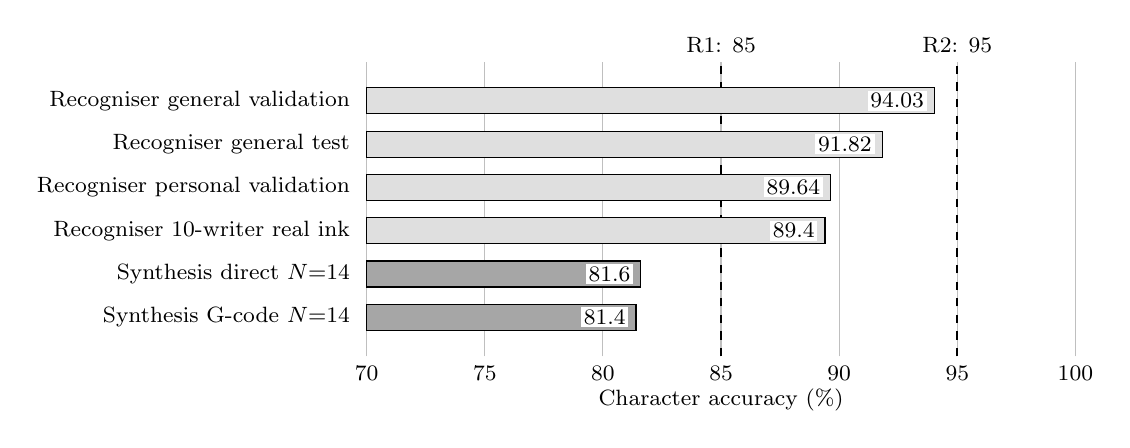
\begin{tikzpicture}[x=0.3cm,y=0.55cm]
\foreach \v in {70,75,80,85,90,95,100}{
  \draw[gray!50] ({\v-70},-0.4) -- ({\v-70},6.4);
  \node[font=\footnotesize,below] at ({\v-70},-0.4) {\v};
}
\node[font=\footnotesize] at (15,-1.4) {Character accuracy (\%)};
\draw[thick,dashed] (15,-0.4) -- (15,6.4);
\draw[thick,dashed] (25,-0.4) -- (25,6.4);
\node[font=\footnotesize,above] at (15,6.4) {R1: 85};
\node[font=\footnotesize,above] at (25,6.4) {R2: 95};
\foreach \lab/\val/\circ [count=\i from 0] in {Recogniser general validation/94.03/0,Recogniser general test/91.82/0,Recogniser personal validation/89.64/0,Recogniser 10-writer real ink/89.4/0,Synthesis direct $N{=}14$/81.6/1,Synthesis G-code $N{=}14$/81.4/1}{
  \pgfmathsetmacro{\yy}{5.5-\i}
  \ifnum\circ=1 \fill[gray!70] (0,{\yy-0.3}) rectangle ({\val-70},{\yy+0.3});
  \else \fill[gray!25] (0,{\yy-0.3}) rectangle ({\val-70},{\yy+0.3}); \fi
  \draw (0,{\yy-0.3}) rectangle ({\val-70},{\yy+0.3});
  \node[font=\footnotesize,anchor=east] at (-0.3,\yy) {\lab};
  \node[font=\footnotesize,anchor=east,fill=white,inner sep=1pt] at ({\val-70-0.3},\yy) {\val};
}
\end{tikzpicture}
\caption{Established character accuracies against the targets of R1 and R2. Light bars: recogniser on the general benchmark and on personal or real-ink data (optimistic splits). Dark bars: synthesised text read by the search judge (circular). The axis starts at 70\%.}
\label{fig:res-bars}
\end{figure}

        \QualificationSection{Observations}

            The circular figures for synthesised text (81.4\% to 81.6\% at $N=14$) lie below 85\%, whereas the server's stored figures (85.8\%, 84.1\%) and the scoped run (92.9\%) lie at or above it; these were obtained with different sentences, writers, tries and sample sizes.
            The genuine handwriting of the scoped run was read at 65.0\% and the synthesised text at 88.2\%.
            No independent evaluation, human panel or overlay distance exists.

        \QualificationSection{Statistical analysis}

            Intervals follow Equation~\ref{eq:res-wilson} and the bootstrap (over pages, writers and matched pairs); the pass criterion is a lower 95\% bound of at least 0.85 for $A_{\mathrm{c}}$ and $\rho$.
            \emph{Expected outcome.}
            Geometric features (slant, character width, ascender/descender ratio) are expected to correlate, because the synthesiser reuses the writer's own letter paths; stroke width and ink density are expected to deviate, because the plotter pen has one line width, so $\rho$ is reported with and without them.
            Overlay distances are expected to be dominated by spacing differences, so the AUC is expected to be clearly above 0.5 but well below 1.0; no numerical outcome is predicted.
            If the independent accuracy is below the circular figures, the quality setting and scoring weights must be re-tuned with an independent judge.

%%%%%%%%%%%%%%%%%%%%%%%%%%%%%%%%%%%%%%%%%%%%%%%%%%%%%%%%%%%%%%%%%%%%%%%%%%%%%%%%%

\medskip
    \QualificationTest{Classification of text and writer from real photographed pages (R2)}
\label{sec:res-qtp2}

        \QualificationSection{Objectives of the test or experiment}

            The test is to prove an overall accuracy of at least 95\% through the whole chain on pages never used for training, checkpoint selection or tuning.
            As the proposal does not define ``overall'', text accuracy $A_{\mathrm{c}}$ (Equation~\ref{eq:res-cacc}) and writer accuracy $A_{\mathrm{w}}$ (fraction of pages assigned to the correct writer) are reported separately and combined as
            \begin{equation}
            \label{eq:res-overall}
            A_{\mathrm{mean}}=\tfrac{1}{2}\left(A_{\mathrm{c}}+A_{\mathrm{w}}\right),\qquad A_{\mathrm{prod}}=A_{\mathrm{c}}\,A_{\mathrm{w}},
            \end{equation}
            where $A_{\mathrm{prod}}$ (both correct) is the criterion and $A_{\mathrm{mean}}$ the lenient reading.

        \QualificationSection{Equipment used}

            The capture rig, the ODROID N2+ with the final server and models, and a printed predefined paragraph; camera and lamp: \textbf{[TO BE COMPLETED BY STUDENT: camera model, resolution, mounting height, lamp type and photograph of the rig]}.

        \QualificationSection{Test setup and experimental parameters}

            The line-level validation split of the personal writers leaks: a random 15\% of lines per page was held out, so lines from the same sheet and session are in both sets (52 of 123 validation lines share pages with training), and the checkpoint was selected on them.
            The fix is new pages kept aside: at least 3 per personal writer, plus the held-out form page of each of the eight database writers, printed and photographed with the rig (about 14 pages, 350 lines).
            Seen lines are scored separately to quantify the leakage; references are double-entered transcripts.

        \QualificationSection{Steps followed in the test or experiment}

            Each frozen photograph is classified through the server without intervention; line text, per-line probabilities and the page-level mean probabilities are recorded, scored, summarised in a $10\times10$ confusion matrix, and the predefined paragraph is then classified live.

        \QualificationSection{Results or measurements}

            Table~\ref{tab:res-r2} lists the established figures, which come from splits that favour the system.

\begin{table}[h]
\centering
\fontsize{10}{12}\selectfont
\begin{tabularx}{\linewidth}{|>{\raggedright\arraybackslash}p{4.3cm}|>{\raggedright\arraybackslash}X|}
\hline
\textbf{Measure} & \textbf{Established figure and caveat, or status} \\
\hline
Recogniser, general benchmark & Validation 94.03\%, test 91.82\% character accuracy (reproduced exactly during analysis); word error rate 21.1\% / 26.7\%. Only the test figure is untouched by checkpoint selection. \\
\hline
Recogniser, personal validation lines & 89.64\%; 15\% of lines per page, optimistic. \\
\hline
Recogniser, 10-writer real ink & 89.4\%; not a clean unseen-writer test. \\
\hline
Writer classifier (ink), real validation pages & 100\%; line-level split inside pages, best checkpoint reported, no separate test set. \\
\hline
Shape classifier, real ink & 96.7\% (119 of 123 lines); the ink classifier reaches about 20\% on synthesised output. \\
\hline
Live check, one personal photograph & Correct writer at 98.6\% confidence, 28 lines detected, accurate transcription (single page, not a statistic). \\
\hline
Held-out pages ($A_{\mathrm{c}}$, $A_{\mathrm{w}}$, $A_{\mathrm{mean}}$, $A_{\mathrm{prod}}$, confusion matrix), paragraph demonstration & \nym{} \\
\hline
\end{tabularx}
\caption{Results for qualification test 2 (design-stage figures, not re-run for this report).}
\label{tab:res-r2}
\end{table}

        \QualificationSection{Observations}

            The recogniser reached 91.82\% (test) and 94.03\% (validation), 3.2 and 1.0 points below 95\%, and 89.64\% on personal lines.
            The word error rates (21.1\%, 26.7\%) are far higher than the character error rates (5.97\% to 8.18\%).
            The shape classifier made four errors on 123 lines.
            No overall accuracy on held-out photographed pages has been measured.

        \QualificationSection{Statistical analysis}

            With 14 pages, a perfect $A_{\mathrm{w}}$ has a Wilson lower bound of only about 78\%, and about 73 error-free pages would be needed for a bound of 95\%; the roughly 350 lines (lower bound about 98.9\% when error-free) are therefore reported as the more powerful but correlated statistic.
            \emph{Expected outcome.}
            Text accuracy on unseen personal handwriting is expected to be below the general-benchmark figure, because only 13 personal pages were available for fitting, so 95\% is not expected for text.
            If $A_{\mathrm{w}}$ is near 100\%, $A_{\mathrm{mean}}$ can exceed 95\% while $A_{\mathrm{prod}}$ does not.
            The writer accuracy on new pages is expected to fall below 100\%, since the ink classifier is sensitive to pen, paper and illumination.

%%%%%%%%%%%%%%%%%%%%%%%%%%%%%%%%%%%%%%%%%%%%%%%%%%%%%%%%%%%%%%%%%%%%%%%%%%%%%%%%%

\medskip
    \QualificationTest{Reproduction time per character (R3)}
\label{sec:res-qtp3}

        \QualificationSection{Objectives of the test or experiment}

            The test is to prove that a sentence of $x$ characters is reproduced within $4x$ seconds,
            \begin{equation}
            \label{eq:res-r3}
            t_{\mathrm{char}}=\frac{T_{\mathrm{syn}}+T_{\mathrm{write}}}{x}\le 4\ \mathrm{s},
            \end{equation}
            where $T_{\mathrm{syn}}$ is the synthesis time, $T_{\mathrm{write}}$ the time from first to last motion and $x$ the number of characters.
            As the proposal does not say whether synthesis counts, both variants are reported; calibration is a one-off step and is reported separately.

        \QualificationSection{Equipment used}

            The ODROID N2+ with the server, the assembled gantry, a stopwatch and logged time stamps at the start and end of synthesis and motion.

        \QualificationSection{Test setup and experimental parameters}

            Tries $N\in\{1,3,6,14,30\}$, sentences of 10, 20, 40 and 80 characters, 5 repetitions (100 syntheses); writing time for the 20 jobs at $N=14$.
            Only figures measured on the ODROID N2+ itself count; laptop figures are indicative.

        \QualificationSection{Steps followed in the test or experiment}

            After one calibration, each job is synthesised, sent and timed by log and stopwatch, $t_{\mathrm{char}}$ is computed from Equation~\ref{eq:res-r3}, and any stall is kept as a failed run.

        \QualificationSection{Results or measurements}

            Table~\ref{tab:res-r3} lists the established figures (laptop and generator model, not valid for the ODROID N2+).

\begin{table}[h]
\centering
\fontsize{10}{12}\selectfont
\begin{tabularx}{\linewidth}{|>{\raggedright\arraybackslash}p{4.5cm}|>{\raggedright\arraybackslash}X|}
\hline
\textbf{Measure} & \textbf{Established figure and caveat, or status} \\
\hline
Best-of-$N$ synthesis, 38 characters, server, loaded laptop & About 105~s (2.8~s per character); text read-back 97.4\%; $N$ not recorded. \\
\hline
Synthesis with 3 tries, laptop & About 5 to 7~s (sentence length not recorded). \\
\hline
Writing time, generator model (11-character word) & 2.4 to 2.8~s per character, about 34\% of it pen dwell; model values only. \\
\hline
Synthesis and writing time on the ODROID N2+; $t_{\mathrm{char}}$ against $N$ and $x$ & \nym{} \\
\hline
\end{tabularx}
\caption{Results for qualification test 3 (laptop and model figures only).}
\label{tab:res-r3}
\end{table}

        \QualificationSection{Observations}

            The laptop synthesis was below 4~s per character, and the 3-try synthesis took far less time (sentence lengths not recorded as equal).
            The model writing time added to the laptop synthesis time exceeds 4~s per character.
            The driver runs pen-up moves at the pen-down feed (single modal feed register), so the real writing time differs from the model.

        \QualificationSection{Statistical analysis}

            Mean, standard deviation and maximum of $t_{\mathrm{char}}$ over 5 repetitions are given per cell and the requirement is tested on the maximum; $T_{\mathrm{syn}}=a+bNx$ is fitted by regression.
            \emph{Expected outcome.}
            Each try renders and scores a candidate, so $T_{\mathrm{syn}}$ should grow linearly with $N$, and the ARM processor is expected to be slower than the laptop by an unmeasured factor.
            R3 is therefore expected to be met at few tries or for writing time alone, and not at $N=14$ if both are added, unless pen dwell, pen-up feed and search cost are reduced (Section~\ref{sec:discussion}).

%%%%%%%%%%%%%%%%%%%%%%%%%%%%%%%%%%%%%%%%%%%%%%%%%%%%%%%%%%%%%%%%%%%%%%%%%%%%%%%%%

\medskip
    \QualificationTest{Classification time (R4)}
\label{sec:res-qtp4}

        \QualificationSection{Objectives of the test or experiment}

            The test is to prove that the time from instruction to displayed text and writer satisfies
            \begin{equation}
            \label{eq:res-r4}
            T_{\mathrm{cls}}\le 2+0.025\,x\ \text{seconds},
            \end{equation}
            where $x$ is the number of handwritten characters; the stage times identify any shortfall.

        \QualificationSection{Equipment used}

            The rig, the ODROID N2+ with the final server, a logging wrapper (monotonic clock) around each stage and a stopwatch; the interface does not display classification time.

        \QualificationSection{Test setup and experimental parameters}

            Pages with $x=40$, about 200 and about 1000, each run 10 times; the budgets are 3.0, 7.0 and 27.0~s.
            Stages: capture, conditioning and segmentation, recognition per line, writer classification, display; the segmentation profile is repeated on the ODROID N2+.

        \QualificationSection{Steps followed in the test or experiment}

            The clocks start at the instruction, stage times and the total are logged, $x$ is counted from the transcript and Equation~\ref{eq:res-r4} is evaluated.

        \QualificationSection{Results or measurements}

            Table~\ref{tab:res-r4} lists the established figures (development laptop, not the ODROID N2+).

\begin{table}[h]
\centering
\fontsize{10}{12}\selectfont
\begin{tabularx}{\linewidth}{|>{\raggedright\arraybackslash}p{4.5cm}|>{\raggedright\arraybackslash}X|}
\hline
\textbf{Measure} & \textbf{Established figure and caveat, or status} \\
\hline
Segmentation of one $2400\times1800$ photograph, pure Python, laptop & 35 to 57~s (loaded at times); line grouping and chain search dominated (about 70\% in the cleanest run), then labelling and box-filter blurs. \\
\hline
Same with two routines in C99 & About 25\% to 32\% faster end to end; the C routines are 84\% to 88\% faster than their Python versions; optional, not deployed. \\
\hline
Recogniser on a PC & 2.6 to 3.1~s per line, about 65 to 75~ms per character. \\
\hline
Capture, classification and total on the ODROID N2+; $T_{\mathrm{cls}}$ for $x=40$, 200, 1000 & \nym{} \\
\hline
\end{tabularx}
\caption{Results for qualification test 4 (laptop figures only).}
\label{tab:res-r4}
\end{table}

        \QualificationSection{Observations}

            Segmentation took 17 to 28 times the 2~s budget in pure Python (12 to 21 times with the C routines).
            For a 40-character line the allowance is 3.0~s, whereas segmentation alone took at least 35~s and recognition about 2.6 to 3.0~s.
            The recogniser time per character is 2.6 to 3.0 times the specified 25~ms.

        \QualificationSection{Statistical analysis}

            Mean, standard deviation, maximum and stage shares over 10 repetitions are reported; the requirement is tested on the maximum.
            \emph{Expected outcome.}
            The ARM processor is expected to be slower than the laptop, so the shortfall on the target is expected to be at least as large, dominated by segmentation; the budget cannot be met without the redesign of Section~\ref{sec:discussion}.
            Recognition alone ($1000\times0.065=65$~s) is expected to miss the full-page budget of 27~s.

%%%%%%%%%%%%%%%%%%%%%%%%%%%%%%%%%%%%%%%%%%%%%%%%%%%%%%%%%%%%%%%%%%%%%%%%%%%%%%%%%

\medskip
    \QualificationTest{Absolute positional accuracy of the gantry (R5)}
\label{sec:res-qtp5}

        \QualificationSection{Objectives of the test or experiment}

            The test is to prove that the absolute positional error of drawn marks is at most 0.5~mm and that a word written twice coincides within that tolerance.
            Software contributions (quantisation, calibration) and hardware contributions (mechanics, homing repeatability, pen compliance) are separated.

        \QualificationSection{Equipment used}

            The gantry with pen and paper, a flat-bed scanner (600 dots per inch, 0.042~mm per pixel), a steel ruler or vernier calipers (0.02~mm) and a printed calibration sheet with a 10~mm grid of crosses.

        \QualificationSection{Test setup and experimental parameters}

            Software part (offline): the step is $1/80=12.5~\mu$m, the quantisation error per axis at most $6.25~\mu$m and the combined worst case $8.8~\mu$m (derived).
            Hardware part: at least 40 crosses drawn 5 times after fresh calibrations, the paper fixed against registration stops, and the same word written twice.
            The error of a cross is $e_i=\lVert\mathbf{p}_i-\mathbf{p}_i^{\mathrm{cmd}}\rVert$ (measured against commanded position referenced to the machine origin); mean, maximum and 95th percentile are reported with the measurement uncertainty (Equations~\ref{eq:res-r5} and~\ref{eq:res-unc} in the Appendix).

        \QualificationSection{Steps followed in the test or experiment}

            After calibration (the direction pin must be seen to change level on reversal) the grid is drawn, scanned with the ruler, evaluated by image analysis, repeated 5 times, and the overlay of the word written twice is produced (Appendix).

        \QualificationSection{Results or measurements}

            Resolution and quantisation values are derived, not measured; all physical measurements are \nym{}.
            During bring-up the X-axis calibration reached the first end-stop, but the direction pin (physical pin 7) was not observed to change level on reversal; this fault was unresolved and is under investigation.

        \QualificationSection{Observations}

            No positional measurement exists.
            The only hardware observation is the direction-pin fault.
            The digital resolution is 40 times finer than the 0.5~mm tolerance.

        \QualificationSection{Statistical analysis}

            The maximum, mean and 95th percentile of $e_i$ over at least 200 points are given with a bootstrap interval; a pass requires the maximum to be at most 0.5~mm, and a result within twice the expanded uncertainty of the limit is inconclusive.
            \emph{Expected outcome.}
            The software contribution is negligible; the error is expected to be dominated by open-loop effects (lost steps, belt stretch, backlash, switch repeatability, pen compliance), none of which has been measured.
            The literature value of 0.3~mm \cite{huang2024} leaves a 0.2~mm margin.
            The test grid must lie within the common work area, since the generator area (200~mm) exceeds the driver's travel (194~mm in X).

%%%%%%%%%%%%%%%%%%%%%%%%%%%%%%%%%%%%%%%%%%%%%%%%%%%%%%%%%%%%%%%%%%%%%%%%%%%%%%%%%

\medskip
    \QualificationTest{Multi-writer storage (R6)}
\label{sec:res-qtp6}

        \QualificationSection{Objectives of the test or experiment}

            The test is to prove that at least 10 writing styles are stored permanently and that any can be selected at random for reproduction.

        \QualificationSection{Equipment used}

            The ODROID N2+ with the server, a laptop browser and the gantry.

        \QualificationSection{Test setup and experimental parameters}

            The eight database and two personal writers; file counts and sizes; persistence by restarting the server and power-cycling the board; 3 writers drawn with a fixed seed.

        \QualificationSection{Steps followed in the test or experiment}

            The listed writers are compared with the stored files, the list is re-read after restart and power cycle, and a short sentence is written in each of the 3 drawn styles.

        \QualificationSection{Results or measurements}

            The server listed 10 writers in a live check; each is stored as a JSON profile with trained weights; sizes: \textbf{[TO BE COMPLETED BY STUDENT: size of each profile and of the weight files]}.
            Persistence and the gantry demonstration are \nym{}.

        \QualificationSection{Observations}

            The list contained 10 entries, equal to the minimum.

        \QualificationSection{Statistical analysis}

            This is a count and pass/fail test; no statistical analysis is appropriate.
            \emph{Expected outcome.}
            Persistence is expected because the profiles are files; the gantry demonstration depends on the fault of qualification test 5.

%%%%%%%%%%%%%%%%%%%%%%%%%%%%%%%%%%%%%%%%%%%%%%%%%%%%%%%%%%%%%%%%%%%%%%%%%%%%%%%%%

\subsubsection*{Field condition checks (FC1 and FC2)}
\label{sec:res-fc}

Neither field condition was measured.
\textbf{FC1:} a lux meter at the page plane records five points (centre and corners of an A4 page); the condition is met if all lie between 400 and 1000~lux, and qualification test 2 is repeated on the same pages at about 200, 700 and 1200~lux.
Illuminance: \nym{}; the flat-field correction and local thresholding should limit degradation within the range, with larger degradation below 400~lux.
\textbf{FC2:} a spirit level or inclinometer on both axes (tilt below $0.5^\circ$) and a logging accelerometer on the frame during a standard job, with the repeat error of qualification test 5 at rest and with a lightly tapped bench.
Tilt and vibration: \nym{}.


\newpage

\section{Discussion}
\label{sec:discussion}

\subsection{Critical evaluation of the design} % REQUIRED HEADING
\label{sec:dis-critical}

This subsection interprets the results of Section~\ref{sec:results}, evaluates the design choices in hindsight and identifies the aspects that must change before the requirements of the proposal can be considered proven.
The results are limited in two ways that determine every conclusion below: the existing figures are design-stage figures obtained on a development laptop, and the evidence on synthesis is circular, because the networks that select the best candidate are the networks that report the score.
Strong statements are therefore avoided where the evidence does not support them.

    \subsubsection{Interpretation of results}
    \label{sec:dis-interp}

        \textbf{R1, reproduction fidelity.}
        The established figures do not allow a conclusion on R1.
        The character accuracies of synthesised text range from 81.4\% to 92.9\% depending on the run, and the writer identification from 91.5\% to 100\%; the runs differ in sample size, number of tries and writers, and all use the judges of the search.
        A best-of-$N$ search that maximises a judge's score necessarily raises that judge's score, so the figures show that the search works, not that a human reader or an independent classifier would agree.
        One observation in the established data limits the meaning of the 85\% target itself: in the scoped run the recogniser read the genuine handwriting of the reference set at 65.0\% and the synthesised text of the same writers at 88.2\%.
        The synthesised text was thus easier for the machine to read than the writer's own text.
        A reproduction that is faithful to the writer, including the writer's irregularities, would be expected to be read less well than a tidy one, so that a high character accuracy and a high stylistic fidelity pull in opposite directions.
        The two parts of R1 must therefore be assessed together, which the qualification test~1 does with independent judges; it is not valid to read the 85\% on legibility as evidence of the 85\% on style.
        The shape-only evaluation supports the conclusion that the synthesiser reproduces writer-specific geometry for most writers (91.5\% for the eight database writers, 6 of 8 above 85\%), but the ten-writer shape-only figure of 78.3\% is as low as the figure of the same judge on the writers' genuine pages (77.5\%), which indicates that the judge, and not the synthesiser, limits that evaluation for several writers.

        \textbf{R2, classification.}
        The recogniser reached 91.82\% on the general test set, 3.2 percentage points below the 95\% target, and 89.64\% on personal validation lines, which are optimistic.
        The target is not met for text, whichever reading of ``overall'' is used, unless the writer accuracy is counted: with $A_{\mathrm{w}}=100\%$ the mean of Equation~\ref{eq:res-overall} would be $(91.82+100)/2=95.9\%$, but the same figures give a product of 91.8\%, and the writer figure is itself optimistic.
        The probable cause of the shortfall is the small amount of training material: 13 personal pages and a public line data set on which a CNN--BiLSTM--CTC network of 3.36 million parameters reaches about 92\%, without a language model or lexicon decoder.
        The word error rate of 21.1\% to 26.7\% shows that errors of single characters spread over many words; a language-model or lexicon decoder is a standard way of using this property, and was not used.
        The writer classifier performed well on real photographs, but its 100\% rests on a split in which lines from training pages are used for validation; the figure shows that the classifier fits the training sheets and pens, and not that it generalises to new sheets.

        \textbf{R3, reproduction time.}
        The synthesis of a 38-character sentence at about 2.8~s per character is below 4~s per character on a laptop, and a three-try synthesis is faster by a large factor.
        The writing time was not measured, and the model of the generator gives 2.4 to 2.8~s per character with 34\% of it spent on the pen dwell.
        The sum of the two exceeds 4~s per character, so the answer depends on an ambiguity of the proposal, which does not state whether synthesis counts: if only the writing time counts, R3 is plausibly met by the model; if both count, it is not met at the high quality setting.
        The result on the ODROID N2+ can only be slower than that on the laptop.

        \textbf{R4, classification time.}
        R4 is not met, and the shortfall is large rather than marginal.
        For a 40-character line the budget is 3.0~s, and the laptop needed at least 35~s for segmentation alone (more than 11 times the budget) and about 2.6 to 3.0~s for recognition (about the whole budget).
        The cause is not the neural network but the image-processing stage, which is written in pure Python and uses an algorithm for the grouping of text lines whose cost dominates the profile (about 70\% of the total in the cleanest run).
        The budget of the proposal assumed a conditioning time of 2~s, which presupposed a considerably simpler algorithm and a language with compiled inner loops.

        \textbf{R5, positional accuracy.}
        No conclusion is possible.
        The step resolution (12.5~$\mu$m) shows only that the control signals are not the limiting factor; the open-loop mechanics determine the error.

        \textbf{R6, storage.}
        R6 is met for storage: ten writers are stored in files, and the number equals the minimum.
        The margin is zero, but the requirement is a minimum.

        \textbf{Conditions under which the requirements could be considered met.}
        R3 could be considered met if the quality setting is limited to a few tries and if the proposal's 4~s per character is read as the writing time of the gantry (or as the sum at a reduced number of tries).
        R2 could be considered met under the lenient mean definition if the independent writer accuracy on new pages is at least 99\%, and under the strict definition only if the text accuracy rises to about 97.5\% (as $A_{\mathrm{prod}}\ge0.95$ requires $A_{\mathrm{c}}A_{\mathrm{w}}\ge0.95$).
        R1 could be considered met if the independent judges of qualification test~1 confirm 85\% for both parts; the established data do not allow this to be assumed.
        R4 cannot be considered met in the present implementation under any reading of the proposal.

    \subsubsection{Critical evaluation}
    \label{sec:dis-crit}

        \textbf{Line-level reading instead of character separation.}
        The design replaced the proposal's character separation by separation into lines and a sequence recogniser.
        This was the right choice for connected handwriting, where character boundaries do not exist, and it makes the accuracy independent of a separation error; the price is that the reading of a line must be done by a network that processes the whole line, and the cost per character is higher than the proposal's 25~ms assumed.

        \textbf{Best-of-$N$ search with the judges inside the loop.}
        The search with a recogniser and a writer classifier as judges was a good decision for quality, because it prevents the synthesis from drawing an illegible or wrong-style sample.
        In hindsight it was a poor decision for verification, because it removed the independence of the evaluation, and for time, because each of the $N$ candidates costs a rendering and two network passes.
        Both are addressed by the qualification protocols, and the time by a lower $N$ or a cheaper first-stage filter.

        \textbf{Pure Python for the segmentation.}
        The proposal required that the processing run on the embedded platform and be written without library functions for the algorithm itself.
        Writing the image processing in Python made the design transparent and correct, but the inner loops of the line grouping and labelling are too slow.
        The C routines reduce the labelling and the box sums by 84\% to 88\%, but the end-to-end effect (25\% to 32\%) is small because the grouping dominates.
        This is the consequence of Amdahl's law: if a fraction $p$ of the time is accelerated by a factor $s$, the total speed-up is $1/((1-p)+p/s)$, and with $p=0.30$ (the share outside the grouping, taking the grouping as 70\%) the total speed-up cannot exceed $3.3$ even if the accelerated part took no time.
        The acceleration was not deployed because the benefit was not decisive.

        \textbf{Open-loop gantry with step counting.}
        Using the stepper motors without encoders is a standard and low-cost choice; its accuracy depends on missed steps, and no sensor reveals them.
        The decision to run the driver without acceleration ramps (the generator models an acceleration of 400~mm/s$^2$, the driver does not execute it) makes the real motion differ from the model, and makes a lost step more likely at the start of a stroke at higher feed.


    \subsubsection{Unsolved problems}
    \label{sec:dis-unsolved}

        The following problems were not solved and must be reported.

        \begin{enumerate}
          \item \textbf{X-axis direction fault.} During hardware bring-up the X-axis calibration reached the first end-stop, but the direction pin (physical pin 7) was not observed to change level when the direction was reversed.
          The fault was unresolved when the project was closed; no cause is claimed, as the evidence does not support one.
          Qualification tests 3 (writing time), 5 and 6 (physical demonstration) depend on its resolution.
          \item \textbf{No measurements on the target hardware.} No timing on the ODROID N2+ and no physical accuracy measurement exists; the figures for R3 and R4 are from a laptop.
          \item \textbf{R4 not met.} The segmentation time and the recognition time per character exceed the specification by more than one order of magnitude and by a factor of about 3, respectively.
          \item \textbf{Optimistic validation of the personal writers.} A line-level split inside pages was used, and the checkpoint was selected on the reporting data; no separate test set exists.
          \item \textbf{Circular synthesis evaluation.} No independent judge or human panel was used.
          \item \textbf{Architecture sweep.} A sweep over widths, depths and learning rates was programmed but no result was kept, so the network layers are those of the published design.
          \item \textbf{Implementation issues of the writing path.} (i) The stroke ordering sorts the text rows by ascending $Y$ coordinate, and with $Y$ upward this writes the bottom line first, while the documentation says reading order. (ii) The acceleration that the generator models is not executed by the driver. (iii) The work area of the generator (200~mm) is larger than the driver's travel between its limits (194~mm in X). (iv) The generator issues the fast feed once, and the driver has a single modal feed register, so that pen-up travel runs at the pen-down feed (900~mm/min instead of 2400~mm/min), which lengthens the job.
          \item \textbf{Missing information.} The hardware documentation (CAD files, photographs, wiring diagram, camera data) and the inconsistent values of the number of tries (14 in the tuning notes, 20 as the server default, 30 mentioned in the interface) are \textbf{[TO BE COMPLETED BY STUDENT: reconcile the values and supply the hardware documentation]}.
          \item \textbf{Training mode.} The proposal planned training on the single-board computer; training is done offline, and the interface has no training function.
          \item \textbf{Display of the classification time} (specified in R4) is not implemented.
        \end{enumerate}

        \textbf{What must change to meet R4.}
        Three measures are required together.
        First, the line grouping (about 70\% of the segmentation time) must be redesigned algorithmically, for example by replacing an exhaustive search over component pairs by neighbourhood queries on a spatial index, if the profile on the ODROID N2+ confirms that the search is the quadratic part; the target is a reduction by a factor of at least 20, because $32~\mathrm{s}$ (70\% of 46~s) must fall to well below 2~s.
        Second, the image must be reduced in resolution before segmentation: halving both dimensions of the $2400\times1800$ photograph reduces the number of pixels by 4, and, as the filters and labelling scale with the pixel count, the share outside the grouping (about 14~s) is expected to fall to about 3.5~s; with the C routines, which are 84\% to 88\% faster (a factor of 6 to 8.3), to about 0.4 to 0.6~s.
        These are projections from the measured ratios and not measurements, and they ignore that the ODROID N2+ is slower than the laptop.
        Third, the recogniser must become about 3 times cheaper per character, for example by a smaller network, by quantising the weights to 8 bit integers or by reducing the sequence length at the output; each of these must be validated against the accuracy loss, since R2 is already under its target.
        The cost per character is approximately proportional to the number of multiply-accumulate operations per line, so a 3-fold reduction of this number would be needed.

        \textbf{What must change for the other requirements.}
        For R2 (text): more personal training pages, an evaluation on held-out pages, and a language-model or lexicon decoder.
        For R1: an independent evaluation and the human panel, and if the independent figure is lower, re-tuning with an independent judge.
        For R3: measurement on the ODROID N2+, correction of the feed register, execution of acceleration or a lower pen dwell, and a lower $N$.
        For R5: resolution of the direction-pin fault, completion of the calibration and execution of qualification test~5.

    \subsubsection{Strong points of the design}
    \label{sec:dis-strong}

        The design has the following strong points, each of which is a consequence of a design decision.
        \begin{itemize}
          \item The reading of whole lines avoids the dependence on a character separation that cannot work for connected handwriting, and the recogniser reached 91.82\% on an independent general test set.
          \item The conditioning stage (flat-field correction, local thresholding, skew correction) was designed so that a photograph with uneven lighting can be used, and the live check on a personal photograph read the correct writer at 98.6\% confidence with 28 lines detected and an accurate transcription.
          \item Writers are represented as compact profile files, so that a new writer is added by a file, and ten writers are stored permanently, satisfying R6.
          \item The use of two judges in the search (text and writer) gives a measurable improvement over a single sample, and the shape classifier solves the problem that an ink-based classifier cannot judge a plotter's constant line width (about 20\% on synthesised output).
          \item The numerical resolution of the gantry (12.5~$\mu$m) is 40 times finer than the tolerance of R5, and the absolute step bookkeeping prevents accumulating rounding errors.
          \item Safety in software: end-stop confirmation (three consecutive samples), software limits and automatic retraction after a trip.
          \item The algorithms are implemented from first principles and documented to a level that allows their analysis, and the established limitations (circularity, optimistic splits) are stated.
        \end{itemize}

    \subsubsection{Expected failure conditions}
    \label{sec:dis-failure}

        The system is expected to fail, or to degrade strongly, under the following conditions.
        \begin{itemize}
          \item \textbf{Lighting.} Illuminance below 400~lux or strongly directional light with shadows violates FC1; the thresholding then merges ink with shadows or loses faint strokes, and the recognition accuracy falls.
          \item \textbf{Page skew and perspective.} Large skew angles or a page that is not flat exceed the range of the skew correction.
          \item \textbf{Non-text regions.} Diagrams, tables and printed text can be segmented as text lines; the text versus non-text scoring reduces but does not exclude this, and the recogniser then produces meaningless characters.
          \item \textbf{Unseen writers.} The writer classifier is a ten-class closed-set classifier; a writer who is not among the ten is assigned to one of the ten classes, because the softmax output cannot express ``none of the above'', so the output is wrong without a warning.
          \item \textbf{Styles outside the glyph library.} A writer whose letter shapes are very different from the stored letter paths (for instance with unusual letters, capitals, digits or symbols that were scarce in the training pages) is reproduced with the nearest stored shape; characters that were never harvested cannot be written in that style.
          \item \textbf{Text with accents, mathematical notation or rare symbols}, which occur in the personal pages, are outside the benchmark vocabulary.
          \item \textbf{Motor stalls and lost steps.} The open-loop gantry has no feedback, so a stall shifts every later mark without any signal.
          \item \textbf{Limit switch failure.} A switch that does not close lets the carriage run against the mechanical stop; the software protection depends on the switches, and a hardware emergency stop that cuts the power does not exist.
          \item \textbf{Long sentences.} The synthesis time grows with the number of characters and tries, so that a long text at a high quality setting would take minutes on the target board and may time out the web request.
          \item \textbf{Network failure} between the browser and the server prevents control of the system; a running job continues on the board.
        \end{itemize}
        The system does not fail gracefully in all cases: the classifier returns a confident answer for an unseen writer, and the gantry cannot detect lost steps.

\subsection{Considerations in the design} % REQUIRED HEADING
\label{sec:dis-considerations}

This subsection addresses the ergonomics, health and safety, environmental, social, legal and ethical aspects of the design.

    \subsubsection{Design ergonomics}

        The user interacts with the system through a web interface with four pages (Read, Write, Model and Style) that run in a browser on any laptop connected to the network, so that no program is installed by the user.
        The Read page captures the page with a live preview and shows the recognised text, the writer and the confidence; the Write page keeps the writing grid locked until the gantry has been calibrated, which prevents a job on an uncalibrated machine; and a preview of the G-code is shown before it is sent.
        The shortcomings are that the live progress of a running job is not displayed, the classification time is not shown, and the interface has no training function.
        The physical rig has to be set up with the page, the pen and the paper placed by hand; the documentation of the rig is incomplete.

    \subsubsection{Health and safety}

        The electronics operate at low voltage (a single-board computer, stepper-driver modules and small motors), so the risk of electric shock is low; \textbf{[TO BE CONFIRMED BY STUDENT: supply voltage and the mains insulation of the power supply]}.
        The mechanical hazards are the moving carriage, belts and pulleys, which present pinch points for fingers while the gantry moves, and the pen, whose tip is not hazardous at the writing force.
        The protective measures are the end-stop switches with confirmation, the software limits and the automatic retraction, and the calibration at a low speed (7.8~mm/s).
        There is no hardware emergency stop that removes the motor power, and the server has no abort function for a running job; a job can be stopped only by ending the program or by removing the power, which is a limitation; and the fitting of a mains-independent emergency stop is recommended for use by others.
        Users must keep their hands away from the carriage while a job runs.

    \subsubsection{Environmental impact}

        The ODROID N2+ is a low-power board, and the stepper motors consume power only while the gantry works, so the energy use is small in comparison with a desktop computer.
        The system uses paper; test pages and failed jobs add waste, which is limited by the preview before writing and by the option to write on used paper.
        The mechanical parts that were printed in plastic or bought as standard parts are \textbf{[TO BE COMPLETED BY STUDENT: which parts were 3D-printed and with which material]}; they can be reused, and plastic and electronic waste at the end of life must be taken to a recycling point and not discarded with domestic waste.
        The pen ink is a small consumable; no hazardous material beyond the electronics is used.
        The system produces no relevant acoustic or electromagnetic emission beyond the stepper motor noise and the pulses of the drive.

    \subsubsection{Social and legal impact}

        The social benefit is that the system can write in a person's own handwriting for those who cannot write neatly or at all, for example because of an injury, and offers the personal touch of handwriting that the proposal identified.
        The technology has also a risk of misuse: reproducing a person's handwriting can be used for forgery or impersonation, for instance on signed documents or letters.
        The risk is reduced, but not removed, by the use of a plotter pen of constant line width, which differs from natural writing in stroke width and pressure (the ink-based classifier identified only about 20\% of the synthesised output, so these ink properties are not reproduced), but a document in a plausible style can still mislead a reader.
        Handwriting samples are personal information, and a writer profile is similar to biometric data, since it permits the identification of the writer; in South Africa the Protection of Personal Information Act (POPIA) applies to such data.
        This requires the consent of the writers, the minimum storage and the protection of the profiles against access by others.
        The samples of the two personal writers require documented consent, \textbf{[TO BE COMPLETED BY STUDENT: confirm that consent was given and in what form]}, and the eight database writers are the contributors to a public research database whose terms of use apply.
        The server has no user accounts (only an optional shared key), accepts requests from any origin and can start physical motion for anyone who can reach its port, so it must be operated only on a trusted local network.
        No other legislation was identified to which a research prototype of this type must conform beyond the general electrical safety rules; \textbf{[TO BE CONFIRMED BY STUDENT: any applicable regulation or university rule]}.

    \subsubsection{Ethics clearance}

        The project used handwriting samples of two named persons and of a public database, and so involves human participants in a limited way.
        The status of ethics clearance is \textbf{[TO BE COMPLETED BY STUDENT: ethics clearance number, or a statement that no clearance was required]}.
        If the human panel of qualification test~1 is carried out, the raters give informed consent and their responses are stored without personal identifiers, and clearance must be confirmed before the panel is run.


\newpage

\section{Conclusion}
\subsection{Summary of the work completed}
\label{sec:con-work}

This report describes work carried out on the design and implementation of a handwriting robot that recognises handwritten text and its writer and reproduces text on paper in the handwriting style of a chosen writer.

A literature survey on handwriting recognition, writer identification, handwriting synthesis and plotter-based writing was completed.
The software was then designed and implemented from first principles in Python: an image-conditioning and text-line segmentation chain, a convolutional and recurrent sequence recogniser trained with connectionist temporal classification, two ten-class writer classifiers, a builder of per-writer style profiles from forced alignment, a trajectory synthesiser with a best-of-$N$ search, a G-code generator and a stepper-motor driver with end-stop calibration and software limits.
These were integrated on the ODROID N2+ single-board computer behind a web server with a browser interface.
The gantry was constructed from purchased components.
The qualification tests that are required to prove each requirement of the proposal were defined (Section~\ref{sec:res-qtp}), but were not executed for this report; the results that exist are design-stage figures obtained on a development laptop.
The hardware bring-up was not completed because of an unresolved fault of the direction signal of the X axis.

\subsection{Summary of observations and findings}
\label{sec:con-findings}

The following findings are supported by the evidence that exists.
\begin{itemize}
  \item The sequence recogniser reached a character accuracy of 91.82\% on the general test set and 94.03\% on the validation set, and 89.64\% on the personal validation lines; the 95\% target of R2 for text was therefore not reached.
  \item The ink-based writer classifier reached 100\% on its validation pages, but this figure is optimistic, because the personal-writer validation lines share pages with the training lines; the shape classifier reached 96.7\% on real ink.
  \item The synthesised text was read with 81.4\% to 92.9\% character accuracy and identified with 91.5\% to 100\% writer accuracy by the judges of the search, which are circular figures; an independent evaluation was designed but not carried out.
  \item The time of classification (R4) was not met on the development laptop: the segmentation took 35 to 57~s against a budget of 2~s, and the recogniser took 65 to 75~ms per character against 25~ms; the grouping of text lines accounted for about 70\% of the segmentation time, and C implementations of two routines reduced the total time by 25\% to 32\% only.
  \item The synthesis of a 38-character sentence took about 105~s (2.8~s per character) on a loaded laptop, and the physical writing time and the positional accuracy of the gantry (R3, R5) were not measured.
  \item Ten writers are stored permanently (R6), and the server lists them.
\end{itemize}
It follows that R6 is met, R4 is not met and the requirements R1 to R3 and R5 are not proven by the existing evidence.
An important implication is that the time requirement can only be met by a redesign of the line-grouping algorithm, a reduction of the image resolution before segmentation and a cheaper recogniser, as quantified in Section~\ref{sec:discussion}; the neural network is not the dominant cost.
A second finding is that a high character accuracy of synthesised text and a faithful reproduction of a writer's style are partly in conflict, because the recogniser read the genuine handwriting of a reference set at 65.0\% and the synthesised text at 88.2\%.

\subsection{Contribution}
\label{sec:con-contribution}

The following was new to the student and was mastered during the project: the training of sequence networks with connectionist temporal classification, the algorithms of the image-conditioning and line-segmentation chain, the extraction of writer-specific letter paths by forced alignment, the synthesis of handwriting trajectories, the generation of G-code and the control of stepper motors from the general-purpose pins of a single-board computer.
All of these were implemented from first principles by the student in Python, and C99 was used for an optional acceleration of two routines.
The mechanical parts, the camera, the single-board computer, the motors and drivers, the end-stop switches, the pen mechanism and the power supply were purchased as finished items and carry no design credit.
The design of the networks follows a published layer pattern \cite{kizilirmak2023}, and public data were used for training.
\textbf{[TO BE COMPLETED BY STUDENT: the interaction with the study leader (how often consulted, what guidance and what direct help were received, for example with the hardware faults), and the contributions of other persons, including any code that was taken from or adapted from other sources and any help received from fellow students or others.]}

\subsection{Suggestions for future work}
\label{sec:con-future}

The work can be continued in the following order of priority.
\begin{enumerate}
  \item Resolve the direction-pin fault of the X axis, complete the calibration and execute the qualification tests 3, 5 and 6 on the gantry, including the field checks FC1 and FC2.
  \item Execute qualification test~2 on newly collected held-out pages, and qualification test~1 with independent judges, a human panel and the hand-crafted and overlay measures, so that the figures of Section~\ref{sec:results} are no longer circular or optimistic.
  \item Redesign the line grouping, reduce the image resolution before segmentation, deploy compiled implementations, and make the recogniser about 3 times cheaper per character (smaller network, quantisation, shorter sequence), measuring each change on the ODROID N2+.
  \item Add a language-model or lexicon decoder and more personal training pages to raise the text accuracy towards 95\%.
  \item Correct the implementation issues of the writing path (reading-order stroke ordering, execution of acceleration, work area, pen-up feed), add a hardware emergency stop and an abort function, and consider a position feedback (for example a sensor on the end-stops or a camera check of the written line) so that lost steps can be detected.
  \item Add an unknown-writer class to the writer classifier, and an authenticated interface.
\end{enumerate}

\newpage

%% Use the IEEE Transactions style for the references.
\bibliographystyle{IEEEtran}
\bibliography{references,refs_w1,refs_w2,refs_w3,refs_w4,refs_w5}
\newpage

%% --- Appendix ------------------------------------------------------------

\eprsec{Appendix}

\newpage
\setcounter{secnumdepth}{0}

\titleformat{\subsection}[display]
{\fontsize{14pt}{16.8pt}\selectfont\bfseries} {} {5pt} {\formatsubsectiontitle}
\titleformat{\subsection}[display]
{\fontsize{14pt}{16.8pt}\selectfont\bfseries} {} {5pt} {\formatsubsectiontitle}

%%
%%  Department of Electrical, Electronic and Computer Engineering.
%%  EPR400/2 Final Report - Technical Documentation.
%%  Copyright (C) 2011-2021 University of Pretoria.
%%

% Appendix material owned by writer 2 (supporting figures, tables and detailed derivations moved out of Sections 3.1 to 3.5)

\subsection{Appendix: Page conditioning and line segmentation (supporting material)}

This part of the appendix contains the supporting figures, the detailed procedures and the design-alternatives table of Section~\ref{sec:segmentation}; the subsection names quoted in that section are the paragraph names below.

\begin{figure}[h]
\centering
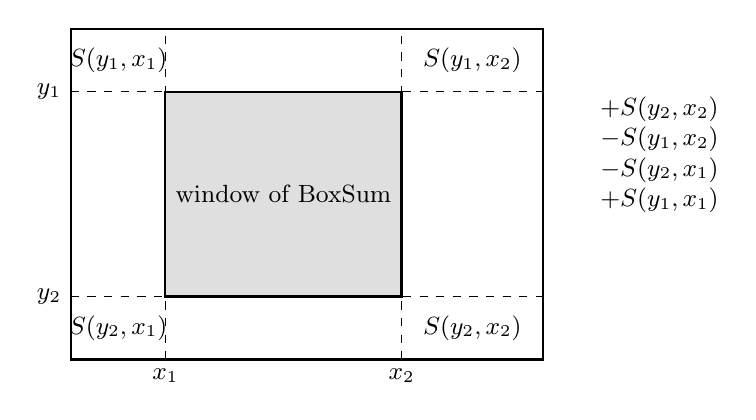
\begin{tikzpicture}[x=1cm,y=1cm]
\fill[gray!25] (1.2,0.8) rectangle (4.2,3.4);
\draw[thick] (0,0) rectangle (6,4.2);
\draw[thick] (1.2,0.8) rectangle (4.2,3.4);
\foreach \x/\l in {1.2/{$x_1$},4.2/{$x_2$}} {\draw[dashed] (\x,0) -- (\x,4.2); \node[font=\small,below] at (\x,0) {\l};}
\foreach \y/\l in {0.8/{$y_2$},3.4/{$y_1$}} {\draw[dashed] (0,\y) -- (6,\y); \node[font=\small,left] at (0,\y) {\l};}
\node[font=\small] at (2.7,2.1) {window of $\mathrm{BoxSum}$};
\node[font=\small] at (0.6,3.8) {$S(y_1,x_1)$};
\node[font=\small] at (5.1,3.8) {$S(y_1,x_2)$};
\node[font=\small] at (0.6,0.4) {$S(y_2,x_1)$};
\node[font=\small] at (5.1,0.4) {$S(y_2,x_2)$};
\node[font=\small,align=left,anchor=west] at (6.6,2.6) {$+S(y_2,x_2)$\\$-S(y_1,x_2)$\\$-S(y_2,x_1)$\\$+S(y_1,x_1)$};
\end{tikzpicture}
\caption{The four-corner rule of the summed-area table. Each table entry $S(y,x)$ is the sum of all pixels above and to the left of $(y,x)$ (measured with the vertical axis pointing down), so the shaded window sum follows from four entries (Equation~\ref{eq:seg-boxsum}).}
\label{fig:seg-boxsum}
\end{figure}

\figplaceholder{5.2cm}{Four panels of the same photograph: (a) colour photograph resized to 2400 px; (b) luma grey image $G$; (c) background estimate $B$ as a heat map; (d) corrected image $I_{\mathrm c}$. Source: run the stages of \texttt{ProcessPage} on a personal page, e.g. \texttt{NOGIT/dylan/preprocessing\_deskew\_ruleline\_border\_cleanup.jpg}, and save the intermediate arrays.}
\caption{Illumination correction. The estimated background (c) follows the lighting gradient of the photograph, and its division from the grey image yields a flat white paper level (d) on which a local threshold is reliable.}
\label{fig:seg-illum}

\figplaceholder{4.6cm}{Page-mask construction as a $2\times3$ panel: Otsu paper candidates, largest component, hole-filled and closed mask, convex-hull notch repair, final eroded mask overlaid on the photograph. Source: stage~2 of \texttt{ProcessPage}.}
\captionof{figure}{Construction of the page mask (placeholder).}
\label{fig:seg-mask}

\begin{figure}[h]
\centering
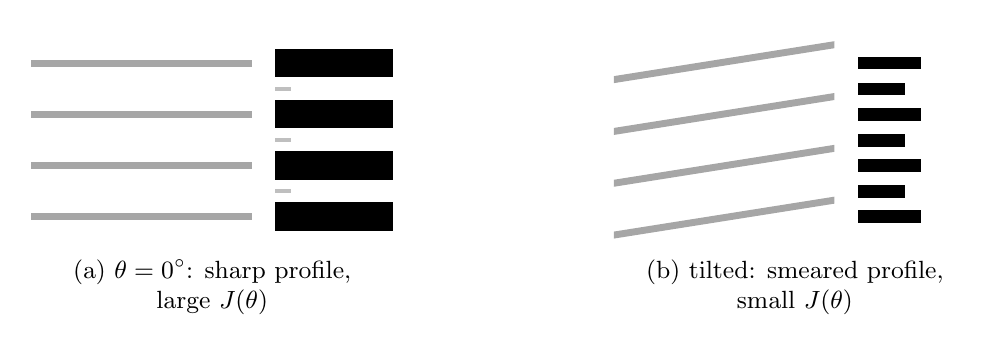
\begin{tikzpicture}[x=1cm,y=1cm]
% left: aligned lines
\begin{scope}
\foreach \k in {0,1,2,3} {\draw[line width=2.5pt,gray!70] (0,\k*0.65) -- (2.8,\k*0.65);}
\foreach \k in {0,1,2,3} {\fill[black] (3.1,\k*0.65-0.18) rectangle (3.1+1.5,\k*0.65+0.18);}
\foreach \k in {0,1,2} {\fill[black!25] (3.1,\k*0.65+0.3) rectangle (3.1+0.2,\k*0.65+0.35);}
\node[font=\small,align=center] at (2.3,-0.9) {(a) $\theta=0^\circ$: sharp profile,\\ large $J(\theta)$};
\end{scope}
% right: tilted lines
\begin{scope}[xshift=7.4cm]
\begin{scope}
\clip (0,-0.4) rectangle (2.8,2.4);
\foreach \k in {0,1,2,3} {\draw[line width=2.5pt,gray!70,rotate around={9:(1.4,1.0)}] (-0.4,\k*0.65) -- (3.2,\k*0.65);}
\end{scope}
\foreach \k in {0,1,2,3} {\fill[black] (3.1,\k*0.65-0.08) rectangle (3.1+0.8,\k*0.65+0.08);}
\foreach \k in {0,1,2} {\fill[black] (3.1,\k*0.65+0.24) rectangle (3.1+0.6,\k*0.65+0.40);}
\node[font=\small,align=center] at (2.3,-0.9) {(b) tilted: smeared profile,\\ small $J(\theta)$};
\end{scope}
\end{tikzpicture}
\caption{Principle of the projection-variance skew search. The bars on the right of each panel represent the row-sum profile of the ink. Aligned lines (a) give strong peaks and empty gaps and therefore a large variance, whereas a tilt (b) fills the gaps.}
\label{fig:seg-skew}
\end{figure}

\figplaceholder{4.4cm}{Skew search on a deliberately tilted photograph: left, plot of $J(\theta)$ for the coarse and fine grids with the chosen angle marked; right, the page before and after rotation with the angle. Source: call the skew estimator with each candidate angle and store the scores.}
\captionof{figure}{Measured skew-search objective $J(\theta)$ (placeholder).}
\label{fig:seg-skewmeas}

\begin{figure}[h]
\centering
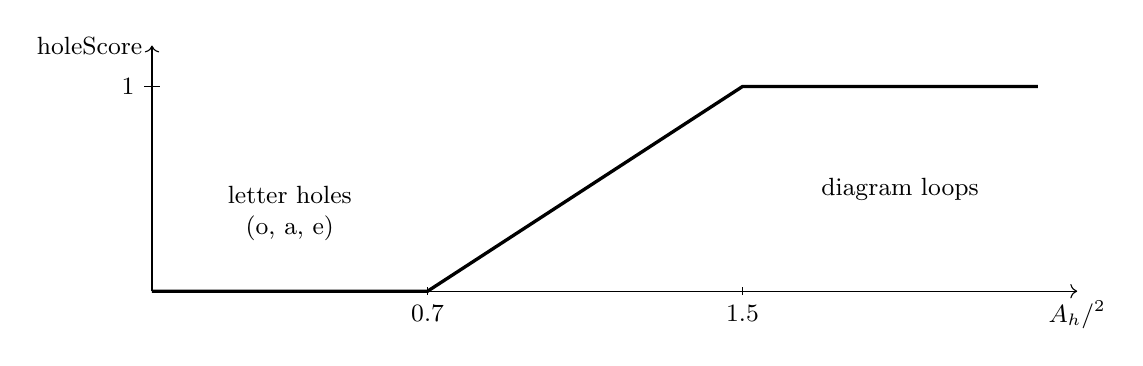
\begin{tikzpicture}[x=5cm,y=2.6cm]
\draw[->] (0,0) -- (2.35,0) node[below,font=\small] {$A_h/\wht^2$};
\draw[->] (0,0) -- (0,1.2) node[left,font=\small] {holeScore};
\draw[very thick] (0,0) -- (0.7,0) -- (1.5,1) -- (2.25,1);
\foreach \xx in {0.7,1.5} {\draw (\xx,0.02) -- (\xx,-0.02) node[below,font=\small] {\xx};}
\draw (0.02,1) -- (-0.02,1) node[left,font=\small] {1};
\node[font=\small,align=center] at (0.35,0.38) {letter holes\\(o, a, e)};
\node[font=\small,align=center] at (1.9,0.5) {diagram loops};
\end{tikzpicture}
\caption{Score ramp of Equation~\ref{eq:seg-mess}. Holes that are smaller than $0.7\wht^2$ are treated as letter counters and give a zero score, holes larger than $1.5\wht^2$ give the maximum score.}
\label{fig:seg-ramp}
\end{figure}

\begin{table}[h]
\centering
\fontsize{9.5}{11.5}\selectfont
\begin{tabularx}{\linewidth}{|p{2.6cm}|X|X|}
\hline
\textbf{Decision} & \textbf{Alternative} & \textbf{Reason for the choice} \\
\hline
Ink threshold & Global fixed or Otsu threshold; local mean and standard-deviation threshold & Photographs have shading of the same order as the ink contrast; division by a blurred background followed by a local mean with offset removes multiplicative and additive variation cheaply. \\
\hline
Blur & Direct Gaussian convolution & Three box means cost $O(1)$ per pixel for any radius with a summed-area table. \\
\hline
Lines & Row projection with gap detection & A projection needs horizontal lines over the full width and cannot separate diagrams; chaining with a baseline curve follows drifting baselines and tags text and non-text. \\
\hline
Skew & Hough transform of edges & Edge directions are dominated by rules and diagrams; the projection variance matches the row grouping that follows. \\
\hline
Rule removal & Long morphological opening & An opening erases long underlines and cross-bars and cannot follow a slope; run-length chaining with a page-crossing requirement protects handwriting. \\
\hline
Faint filtering & Fixed darkness cut-off & Pen pressure and lighting differ per page; Otsu on the component darkness calibrates itself. \\
\hline
Text versus diagram & Learned layout detector & Outside the own first-principles scope and unnecessary for the pages of this project. \\
\hline
Page geometry & Four-point perspective warp & Not implemented; the camera looks straight down at the page, so keystone is small. \\
\hline
\end{tabularx}
\caption{Design alternatives of the segmentation block.}
\label{tab:seg-alt}
\end{table}

\paragraph{Stage 2 details.}
The mask is built in ten steps.
\begin{enumerate}
\item A grey image $G_b$ blurred with nominal scale 4 and the saturation of the hue--saturation--value (HSV) colour model, $S=255(\max_c-\min_c)/\max_c$ (maximum and minimum over the colour channels) are computed.
\item A global threshold $t^*$ is found by the method of Otsu \cite{otsu1979}, which maximises the between-class variance of the intensity histogram,
(equation as in the main text)
where $\omega_B(t)$ and $\omega_F(t)$ are the numbers of pixels below and above $t$, and $\mu_B(t)$ and $\mu_F(t)$ the mean intensities of the two classes (the normalisation $1/N^2$ is omitted because it does not change the arg max).
A global threshold is appropriate here because the paper--desk contrast is large.
\item The candidate set ``paperish'' is $\{G_b\ge t^*\}\wedge\{S<90\}$ (paper is bright and has low saturation); it is opened with a $9\times9$ square and only the largest 4-connected component is kept.
\item To admit parts of the sheet that lie in shadow, the threshold is re-derived from the paper itself: with $m_p$ the median of $G_b$ over the current mask, the set $\{G_b\ge m_p-50\}\wedge\{S<90\}$ is opened and its largest component kept.
\item Holes are filled (background components that do not touch the frame border), the mask is closed with a $15\times15$ square, and holes are filled again.
\item Ragged protrusions (fingers, shadows) are trimmed by a profile test on each axis: with $p$ the mask-sum profile, only samples with $p\ge 0.30\,\mathrm{median}(p\,|\,p>0.2\max p)$ are kept and the largest contiguous run is retained. The factor 0.30 is deliberately low so that a page that is cut off by the frame is not trimmed.
\item Rows and columns darker than the cut level of Equation~\ref{eq:seg-dark}
\begin{equation}
c=\min\!\bigl(m_p-45,\;\max(m_p-85,\;\tfrac12(m_p+m_{bg}))\bigr)
\label{eq:seg-dark}
\end{equation}
are trimmed, where $m_p$ is the median blurred brightness inside the mask and $m_{bg}$ that outside; a page edge in soft shadow (about 0.7 of the paper brightness) is still far brighter than the desk, so the cut level is placed relative to what actually lies off the page.
\item \emph{Shadow-notch repair.} A photographed sheet is a convex quadrilateral, so a concave notch in the mask is a shadow artefact. Each column and row of the mask is made contiguous between its first and last mask pixel, the convex hull of the result is filled, and new pixels are accepted only if $G_b\ge0.55\,m_p$; holes are then filled again.
\item The mask is eroded by a square of odd side $k=2\lfloor e/2\rfloor+1$ with $e=\max(4,\lfloor0.006\min(H,W)\rfloor)$ (about 11 pixels), so that the paper edge itself is not binarised as ink.
\item If the mask covers less than 15\,\% of the frame or no component exists, the mask is set to the whole frame, because abandoning page detection is safer than losing the page.
\end{enumerate}
The method fails for strongly tinted paper (saturation above 90), when the desk is almost as bright as the paper, or when the sheet violates the convexity assumption, and the fallback then applies. Figure~\ref{fig:seg-mask} is reserved for an example of the construction of the mask.


\paragraph{Stage 6 details.}

Ruled paper and other printed structure joins words and lines into giant components, so these structures must be removed \emph{without} removing handwriting that touches them.
Four removal steps are applied in sequence; each is rule-aware or scale-aware so that they act only on components that cannot be handwriting.

\paragraph{Rules by run lengths and chaining.}
For each ink pixel $p$ the length $h\mathrm{Run}(p)$ of its horizontal run and $v\mathrm{Run}(p)$ of its vertical run are computed (the runs are computed for all pixels at once from the row differences).
A minimum rule length $L_r=\max(50,\lfloor3.5\wht\rfloor)$ is defined, the rule thickness is the median vertical run $T=\mathrm{median}(v\mathrm{Run}\,|\,h\mathrm{Run}\ge L_r)$ (2 pixels if none exists), and the thickness cut is $\kappa=\max(4,\lfloor1.8T\rfloor)$.
Horizontal rule fragments (Equation~\ref{eq:seg-cand}) are the pixels
\begin{equation}
\mathrm{cand}_H=\bigl(h\mathrm{Run}\ge\max(20,\lfloor0.8\wht\rfloor)\bigr)\wedge\bigl(v\mathrm{Run}\le\kappa\bigr),
\label{eq:seg-cand}
\end{equation}
and vertical candidates are defined symmetrically.
A rule that is broken by crossing strokes or slightly sloped is not one long run, so fragments are chained: the candidate mask is labelled, the components are sorted by $x$, and two components $a$ and $b$ are united if their gap $g=x_b-(x_a+w_a)\le2.5\wht$, their vertical offset satisfies the condition of Equation~\ref{eq:seg-slope}
\begin{equation}
|c_{y,b}-c_{y,a}|\le\Delta_{\max}=2\kappa+0.08\max(0,g)+0.04\,(w_a+w_b),
\label{eq:seg-slope}
\end{equation}
and their darkness differs by at most 55 grey levels ($c_y$ is the centroid row, $w$ the component width, and the allowance grows with the distance so that gentle slope and wobble are tolerated).
A group is declared a rule only if it spans at least $0.6W$ (vertical rules: $0.45H$) and reaches both ends of the page, $x_1\le0.15W$ and $x_2\ge0.85W$ (vertical: $0.2H$ and $0.8H$).
A long word or underline cannot satisfy this condition.
The rule mask is the union dilated by $3\times3$, restricted to pixels with $v\mathrm{Run}\le\kappa+2$ or $h\mathrm{Run}\le\kappa+2$ so that thick pen strokes that cross the rule are not deleted.
Two passes are run, the second catching rules that were hidden behind the first layer or split.
An elongated underline is not a rule: a component is \emph{underline-like} if its width exceeds $4\wht$ and its mean thickness (area over width) is at most 6.5 pixels.

\paragraph{Faint components, rule-aware.}
Components that are fainter than the handwriting (leftover printed rules, bleed-through, shadows) are identified without a fixed threshold.
Candidates are the components with width $>8\wht$, height between $0.25\wht$ and $8\wht$, fill ratio (area over bounding-box area) below 0.2 and a largest enclosed hole of at most $1.4\wht^2$ (a drawing has holes, a rule network does not).
Because a word may be glued to a faint rule, the rule is cut out first: a column is \emph{thin} if its vertical ink span is at most $\max(6,\lfloor0.35\wht\rfloor)$, and each run of at least $\lfloor2\wht\rfloor$ consecutive thin columns is removed; this test is insensitive to the slope of a rule.
For each remaining component the darkness of Equation~\ref{eq:seg-dark2}
\begin{equation}
d=255-P_{25}\bigl(I_{\mathrm c}\,\big|\,\text{component}\bigr)
\label{eq:seg-dark2}
\end{equation}
is computed, where $P_{25}$ is the 25th percentile of the corrected intensity inside the component.
If the 90th and 10th percentiles of $d$ over all components differ by less than 60 the page has no bimodality and nothing is removed; otherwise a one-dimensional Otsu threshold $\tau$ (Equation~\ref{eq:seg-otsu} on 64 histogram bins of $d$) separates faint from normal components, and components with $d<\tau$ are removed, unless $\tau$ lies outside $(P_{10},P_{90})$.
The page therefore defines for itself what ``faint'' means, which suits the differences in pen pressure and lighting between pages; an earlier fixed darkness filter was replaced because it removed words together with the faint rule.
Components that were removed here are re-attached later if they lie on a text line (stage 8).

\paragraph{Page edges and facing pages.}
Junk that touches the left or right edge of the page mask or a corner of it (binding shadows, edge noise) is removed: with $t_x=\max(8,\lfloor0.75\wht\rfloor)$ and $t_c=\lfloor2\wht\rfloor$, a component is removed if it is narrower than $0.15W$ and touches a side edge within $t_x$, or if it touches a side edge and a top or bottom edge within $t_c$ while being narrower than $0.25W$ and lower than $3\wht$.
Ink of a facing page that appears at the image border is found from the column ink profile $c(x)$: after smoothing with a box of width $\max(5,\lfloor\wht\rfloor)$ (made odd), columns above $0.25$ times the median of the ``lively'' columns (those above 5\,\% of the maximum) form blocks, the block with the most ink is dominant, and a smaller block that touches the border zone of $2\wht$ is cut away together with half a glyph height of margin; interior blocks such as margin numbers are retained.

\paragraph{Sparse rule networks.}
Sloped or wavy rules are cut into short runs that the test above misses.
For components with width $>6\wht$, height between $1.2\wht$ and $8\wht$, fill ratio below 0.10 and no large hole, the column-span test is applied with the same thin-column definition and run length $\lfloor2\wht\rfloor$.


\paragraph{Grouping details.}
For each chain the points $(c_x,c_y,A)$, sorted by $x$, give a baseline curve whose ordinate is smoothed by an area-weighted average over a five-point window (Equation~\ref{eq:seg-curve}),
(equation as in the main text)
where $y_k$ and $A_k$ are the centroid row and area of the $k$th point (the window is truncated at the ends), and the curve $y_{\mathrm{curve}}(x)$ is linearly interpolated between the points and constant beyond the ends.
Chains of one physical row are merged in three passes.
\emph{Pass 1} (same local height): chains sorted by mean curve height are merged when they overlap in $x$ and the mean difference of the two curves sampled at seven equally spaced positions of the overlap is below $0.6\wht$, or, if they do not overlap, when the curves differ by less than $0.55\wht$ at the middle of the gap; after each merge the scan restarts.
\emph{Pass 2} (pitch-aware): the line pitch $p$ is the median of the consecutive chain-centre gaps that exceed $0.5\wht$ (fallback $1.8\wht$), and chains are merged when the mean curve difference is below $0.45\,p$ (overlapping) or $0.4\,p$ (not overlapping).
Letting the threshold scale with the measured line spacing handles writing of varying size without manual tuning.
\emph{Pass 3} demotes weak chains: a chain is \emph{strong} if it has at least three components, or a width of at least $3\wht$ and an area of at least $2\wht^2$, or if no other chain lies within $0.8\,p$; the components of weak chains re-enter in the next step.

\paragraph{Leftover components.}
Every component that is not yet in a chain is assigned according to its shape.
An underline-like component is attached to the chain whose curve lies above it by between $-0.2\wht$ and $1.5\wht$.
A component with $h\le1.8\wht$ (dots, accents, punctuation) joins the nearest chain curve within $1.3\wht$, where the distance is $|y_{\mathrm{curve}}(c_x)-c_y|$ plus 0.15 pixel per pixel that the component lies outside the chain's $x$-span, unless it overlaps a \texttt{MESS} block.
A taller component, typically an ascender or descender that links two rows, is split \emph{pixel-wise}: every pixel goes to the nearest chain within $2.5\wht$, and each chain receives its sub-mask if it has at least 8 pixels, so that one connected stroke can be shared by two lines.
A chain finally becomes a line unless its total area is below $0.35\wht^2$, its tallest component below $0.35\wht$, or it consists of at most three small solid blobs of total width below $3.5\wht$ (stray dots).
Text lines whose bounding box lies more than 70\,\% inside the core box of a \texttt{MESS} block are absorbed into that block, so that labels inside a diagram are not exported as lines.

\paragraph{Refinement.}
A refinement step rejoins a physical row that chaining split, for example because of a word gap larger than $6\wht$.
With cap $\min(0.5\,p,1.6\wht)$, two lines whose centres differ by at most $0.75\,p$ are merged if one of four signals holds: (i)~the centres differ by less than $0.5\wht$; (ii)~their vertical ranges overlap by at least 70\,\% of the shorter range, centres differ by less than $0.45\,p$ and the smaller line has an area below $4\wht^2$; (iii)~they overlap in $x$ by at most 55\,\% of the narrower width and their curves, evaluated at the middle of the overlap, differ by less than the cap; or (iv)~centres differ by less than $0.6\,p$ and less than 30\,\% of the columns of the narrower line are shared with the other (words interleave along $x$, whereas stacked rows always share columns).
Underline-shaped components that lie at least $0.5\wht$ above their line's curve are moved to the line below which they sit, because an underline belongs to the text written above it, and pale components that were removed as faint are re-attached to the nearest curve when they lie within $0.75\wht$ of it.
The \texttt{TEXT} and \texttt{MESS} items are finally sorted by their vertical centre; a \texttt{MESS} item that is immediately followed by a \texttt{TEXT} item whose centre falls in the top 40\,\% of the block is swapped with it, so that a caption precedes its diagram.



\subsection{Appendix: Text recogniser (supporting material)}

This part of the appendix contains the supporting figures and tables of Section~\ref{sec:textrec}: the layer table, the LSTM cell, the pre-processing schematic, the data sets, the training stages, the forgetting experiment, the alternatives and the details of the inference implementation.

\begin{figure}[h]
\centering
\begin{tikzpicture}[x=1cm,y=1cm]
\draw[thick,fill=gray!15] (0,2.2) rectangle (5.6,3.3);
\node[font=\small] at (2.8,2.75) {line crop: $w\times h$ pixels, variable};
\draw[w2arr] (2.8,2.1) -- (2.8,1.4) node[midway,right,font=\small] {scale by $s$, Equation~\ref{eq:rec-resize}};
\draw[thick] (0,0) rectangle (8,0.8);
\draw[thick,fill=gray!15] (0,0.1) rectangle (5.6,0.7);
\node[font=\small] at (2.8,0.4) {scaled line $w'\times h'$};
\node[font=\small] at (6.8,0.4) {white padding};
\node[font=\small,anchor=east] at (-0.1,0.4) {64};
\node[font=\small,anchor=north] at (4,-0.05) {640 pixels};
\draw[<->] (-0.05,0) -- (-0.05,0.8);
\node[font=\small,align=left,anchor=west] at (8.5,0.4) {ink $\rightarrow+1$\\ paper $\rightarrow-1$};
\end{tikzpicture}
\caption{Pre-processing of a line crop. The crop is scaled uniformly, left-aligned on a white canvas and normalised to the range $[-1,1]$ (Equation~\ref{eq:rec-norm}).}
\label{fig:rec-canvas}
\end{figure}

\begin{table}[h]
\centering
\fontsize{9.5}{11.5}\selectfont
\begin{tabular}{|l|l|r|}
\hline
\textbf{Layer} & \textbf{Output shape} & \textbf{Trainable parameters} \\
\hline
Input & $1\times64\times640$ & 0 \\
Conv 3$\times$3 (1$\to$32), BN, ReLU & $32\times64\times640$ & 384 \\
Conv 3$\times$3 (32$\to$32), BN, ReLU & $32\times64\times640$ & 9\,312 \\
Max-pool 2$\times$2 & $32\times32\times320$ & 0 \\
Conv 3$\times$3 (32$\to$64), BN, ReLU & $64\times32\times320$ & 18\,624 \\
3$\times$ Conv 3$\times$3 (64$\to$64), BN, ReLU & $64\times32\times320$ & 111\,168 \\
Max-pool 2$\times$2 & $64\times16\times160$ & 0 \\
Conv 3$\times$3 (64$\to$128), BN, ReLU & $128\times16\times160$ & 74\,112 \\
5$\times$ Conv 3$\times$3 (128$\to$128), BN, ReLU & $128\times16\times160$ & 739\,200 \\
Height max-pool & $128\times1\times160$ & 0 \\
BiLSTM layer 1 (128$\to$256, 2 directions) & $160\times512$ & 790\,528 \\
BiLSTM layer 2 (512$\to$256, 2 directions) & $160\times512$ & 1\,576\,960 \\
Linear (512$\to$75) & $160\times75$ & 38\,475 \\
Log-softmax & $160\times75$ & 0 \\
\hline
\textbf{Total} & & \textbf{3\,358\,763} \\
\hline
\end{tabular}
\caption{Layer-by-layer shapes and trainable parameters of the text recogniser (batch dimension omitted). Batch normalisation also stores 2\,176 non-trainable running statistics, and the checkpoint therefore holds 3\,360\,951 numbers (13.4\,MB as 32-bit floating point).}
\label{tab:rec-layers}
\end{table}

\begin{figure}[h]
\centering
\begin{tikzpicture}[x=1cm,y=1cm]
\draw[thick,rounded corners=3pt] (0,0) rectangle (8,3.6);
\node[w2box,minimum width=1cm] (f) at (1.4,1.2) {$\sigma$};
\node[w2box,minimum width=1cm] (i) at (3.0,1.2) {$\sigma$};
\node[w2box,minimum width=1cm] (g) at (4.6,1.2) {$\tanh$};
\node[w2box,minimum width=1cm] (o) at (6.6,1.2) {$\sigma$};
\node[font=\scriptsize] at (1.4,0.55) {$f_t$};
\node[font=\scriptsize] at (3.0,0.55) {$i_t$};
\node[font=\scriptsize] at (4.6,0.55) {$g_t$};
\node[font=\scriptsize] at (6.6,0.55) {$o_t$};
\draw[thick,-{Stealth}] (-0.8,3.0) -- (8.8,3.0) node[right,font=\small] {$c_t$};
\node[font=\small,left] at (-0.8,3.0) {$c_{t-1}$};
\node[w2dark,circle,inner sep=1pt] (m1) at (1.4,3.0) {$\odot$};
\node[w2dark,circle,inner sep=1pt] (a1) at (3.8,3.0) {$+$};
\node[w2dark,circle,inner sep=1pt] (m2) at (3.8,2.1) {$\odot$};
\node[w2box,minimum width=0.9cm] (th) at (6.6,3.0) {$\tanh$};
\node[w2dark,circle,inner sep=1pt] (m3) at (6.6,2.1) {$\odot$};
\draw[w2arr] (f) -- (m1);
\draw[w2arr] (i) |- (m2); \draw[w2arr] (g) |- (m2); \draw[w2arr] (m2) -- (a1);
\draw[w2arr] (o) -- (m3); \draw[w2arr] (th) -- (m3);
\draw[w2arr] (m3) -- ++(0,-2.6) -- ++(0,0);
\node[font=\small,anchor=west] at (7.0,2.1) {$h_t$};
\node[font=\small,anchor=north] at (4.0,-0.2) {inputs of all four gates: $[x_t,\,h_{t-1}]$};
\end{tikzpicture}
\caption{Schematic of an LSTM cell (Equation~\ref{eq:rec-lstm}). The memory line $c_t$ at the top is changed only by the forget gate (multiplication) and the input gate (addition), which allows information to travel over many time steps.}
\label{fig:rec-lstm}
\end{figure}

\begin{table}[h]
\centering
\fontsize{9.5}{11.5}\selectfont
\begin{tabularx}{\linewidth}{|p{2.8cm}|p{3.6cm}|X|}
\hline
\textbf{Data set} & \textbf{Split rule} & \textbf{Caveat on the validation figure} \\
\hline
Lines segmented by the student's own block from scanned database pages, with labels generated by alignment (first stage only) &
The last labelled page of every writer is held out. &
Same writers in training and hold-out, so the figure is writer-dependent; the labels are project-generated and noisy. \\
\hline
Public line-level IAM transcription set: 6\,482 training, 976 validation, 2\,915 test lines (6\,481, 976 and 2\,915 after label cleaning) &
Official training, validation and test partitions. &
The validation set drives learning-rate decay and checkpoint choice, so its accuracy is mildly optimistic; the test set is used for no decision. The partitions are believed, but not verified, to be writer-independent, and the warm start from the first stage may have seen some of the same forms. \\
\hline
13 photographed pages of the two personal writers (8 and 5 pages), 355 transcription lines of which one is a diagram marker &
Per page, 15\,\% of the lines (at least one) are drawn at random with a fixed seed as validation; about 52 validation lines in total. &
Validation lines come from the same pages, pen, paper, lighting and vocabulary as training lines; the figure measures ``same writer, same notebook, new lines'' and is optimistic. It also takes part in checkpoint selection. \\
\hline
Ten-author hold-out (eight database writers and the two personal writers) &
Used only as an evaluation set. &
The held-out database lines may have been seen in the line-level training data, and their labels are project-generated, so the figure is not a writer-independent measure. \\
\hline
\end{tabularx}
\caption{Data sets of the text recogniser and their leakage assessment.}
\label{tab:rec-data}
\end{table}

\begin{table}[h]
\centering
\fontsize{9.5}{11.5}\selectfont
\begin{tabularx}{\linewidth}{|l|l|l|l|l|l|X|}
\hline
\textbf{Stage} & \textbf{Data} & \textbf{$\eta_0$} & \textbf{Batch} & \textbf{Epochs} & \textbf{Clip} & \textbf{Schedule and selection} \\
\hline
Base & own lines & $10^{-3}$ & 16 & $\le200$ & none & halve after 5 stalls; stop after 15; up to 3 restarts from the best weights; best validation loss \\
\hline
Clean labels & public set & $10^{-3}$ & 16 & $\le200$ & none & as above, up to 8 restarts; best public validation loss \\
\hline
Personal & personal lines & $3\!\times\!10^{-4}$ & 8 & 60 & 5 & halve after 5 stalls; best personal validation loss \\
\hline
Joint & both, $f=0.20$ & $5\!\times\!10^{-4}$ & 16 & 30 & 5 & halve after 4 stalls on the sum of both validation losses; best $\min$ of the two accuracies \\
\hline
\end{tabularx}
\caption{Hyper-parameters of the four training stages. All stages use RMSprop (Equation~\ref{eq:rec-rmsprop}) with weight decay $10^{-5}$; the minimum learning rate was $10^{-5}$ or $10^{-6}$.}
\label{tab:rec-stages}
\end{table}

\begin{table}[h]
\centering
\fontsize{9.5}{11.5}\selectfont
\begin{tabular}{|l|r|r|r|}
\hline
\textbf{Training} & \textbf{Public val./test (\%)} & \textbf{Personal val. (\%)} & \textbf{Remark} \\
\hline
Clean-label stage only & 93.87 / 91.60 & -- & before personal data \\
Personal only, all layers & 84.26 / 80.56 & 90.2 & forgetting \\
Personal only, frozen convolutions & 85.87 / 82.62 & 88.5 & forgetting \\
Joint (deployed) & 94.03 / 91.82 & 89.64 & both domains kept \\
\hline
\end{tabular}
\caption{The catastrophic-forgetting experiment: character accuracies of the three ways of adding personal data.}
\label{tab:rec-forget}
\end{table}

\begin{table}[h]
\centering
\fontsize{9.5}{11.5}\selectfont
\begin{tabularx}{\linewidth}{|p{3.2cm}|X|X|}
\hline
\textbf{Alternative} & \textbf{For} & \textbf{Against} \\
\hline
Character segmentation and a per-character classifier (small convolutional network) &
Simple network; the proposal's plan. &
Needs a segmenter that works on joined letters; classification errors cannot be repaired by context; needs character-level labels that the available data lack. \\
\hline
Line-level CNN-BiLSTM-CTC (chosen) &
No segmentation below the line; alignment-free training from line transcriptions; context from both sides; output is a string; 3.36 million parameters can be run by a from-scratch implementation. &
Needs line segmentation; greedy decoding leaves spelling errors; CTC assumes independent steps. \\
\hline
Lexicon or language-model decoding &
Repairs near-miss words; gives the lowest error in the published design. &
Needs a corpus and a decoder; the technical vocabulary and symbols of the pages are largely out of vocabulary. Future work. \\
\hline
Deeper backbones with skip connections &
Easier training of very deep networks. &
The 12-layer network with batch normalisation trained well; larger models cost memory and time on the single-board computer. \\
\hline
Attention-based encoder--decoder or transformer &
Strong accuracy on large corpora. &
Far more parameters, large pre-training data, slow autoregressive decoding that can skip or invent text, and hard to implement from scratch for the board. \\
\hline
Word-level recognition &
Uses the lexicon directly. &
Needs word segmentation and a closed vocabulary; poor for names, numbers and symbols. \\
\hline
\end{tabularx}
\caption{Alternatives to the line-level recogniser.}
\label{tab:rec-alt}
\end{table}

\paragraph{Text recogniser: weight file and inference details.}

Training needs a large software environment, which should not be installed on the single-board computer.
The student therefore wrote a separate, from-scratch inference implementation in Python that reads the trained weights directly and uses only array arithmetic.
It consists of three small modules (about 480 lines in total): the layer functions, the network, and a weight reader.

\paragraph{Convolution as a matrix product.}
Each convolution is converted to one matrix multiplication (the im2col method).
The padded input is cut into overlapping $3\times3$ patches, and every patch is flattened into one column of a matrix $\mathrm{cols}\in\mathbb R^{(C_{\mathrm{in}}k^2)\times(H_{\mathrm{out}}W_{\mathrm{out}})}$; with the weights reshaped to $\tilde W\in\mathbb R^{C_{\mathrm{out}}\times C_{\mathrm{in}}k^2}$,
(equation as in the main text)
where $b\,\mathbf 1^\top$ adds the bias of each output channel to all positions.
In Equation~\ref{eq:rec-im2col}, one optimised matrix product replaces the six nested loops of Equation~\ref{eq:rec-conv} and was found to be about ten times faster than a general summation routine, with a difference of about $10^{-13}$ between the two.
The cost is memory: the largest matrix, for the second convolution of stage 1, has $288\times40\,960$ entries (47\,MB as 32-bit floating point), and the largest activation tensor is 5.2\,MB, so the working set is a few tens of megabytes.
Batch normalisation is applied in its folded form of Equation~\ref{eq:rec-bnfold}, pooling uses windowed views of the array, the height collapse is a maximum over one axis, and the LSTM is an explicit loop over the 160 steps with one product of $1024$ rows per step and direction, the backward direction being a pass over the reversed sequence.

\paragraph{Reading the trained weights.}
The training-time weight file is an archive that contains a serialised object structure, in which every tensor is replaced by a reference to a storage key, and one raw little-endian byte file per storage.
The student's weight reader opens the archive, parses the object structure with a customised reader that intercepts the tensor and storage constructors, reads the bytes of each storage into an array, rebuilds every tensor from its shape and strides, and returns a dictionary of 102 arrays with the names of the training model.
The inference code then indexes the weights by name, and no machine-learning software is needed at run time.

\paragraph{Agreement with the training code and cost.}
For one random $64\times640$ input, the largest difference between the $160\times75$ log-probability matrices of the inference code and the training code was $2.3\times10^{-5}$ for the deployed weights, $1.1\times10^{-5}$ for the clean-label stage and $9.5\times10^{-6}$ for the personal stage, with identical arg-max (and therefore decoded text) at all 160 steps; this is a single synthetic input and not a test-set sweep.
The weights occupy 13.4\,MB.
On the development computer (processor only) one forward pass of one line took 2.6 to 3.1\,s; for a line of 40 characters this is about 65 to 75\,ms per character, which exceeds the 25\,ms per character that requirement R4 allows, and the ARM processor of the single-board computer is expected to be slower.
\textbf{[TO BE COMPLETED BY STUDENT: measure the recognition time per line on the ODROID N2+; the project files contain no such measurement, and the proposal's budget may refer to the whole classification step.]}
Optional compiled replacements for the convolution and the LSTM exist but are not used: the compiled convolution was slower than the optimised matrix product on a desktop processor, and the compiled LSTM was 2.8 to 4.4 times faster than the array version.



\subsection{Appendix: Writer identification (supporting material)}

This part of the appendix contains the layer table, the data and training tables, the real stroke-normalisation example and the aggregation diagram of Section~\ref{sec:writerid}.

\begin{table}[h]
\centering
\fontsize{9.5}{11.5}\selectfont
\begin{tabular}{|l|l|r|}
\hline
\textbf{Block} & \textbf{Output shape} & \textbf{Trainable parameters} \\
\hline
Stage 1 (2 conv units, 32 channels) & $32\times64\times640$ & 9\,696 \\
Max-pool 2$\times$2 & $32\times32\times320$ & 0 \\
Stage 2 (4 conv units, 64 channels) & $64\times32\times320$ & 129\,792 \\
Max-pool 2$\times$2 & $64\times16\times160$ & 0 \\
Stage 3 (6 conv units, 128 channels) & $128\times16\times160$ & 813\,312 \\
Height max-pool and width mean-pool & 128 & 0 \\
FC 128$\to$96, ReLU, dropout & 96 & 12\,384 \\
FC 96$\to$10 & 10 & 970 \\
\hline
\textbf{Total} (backbone 952\,800, head 13\,354) & & \textbf{966\,154} \\
\hline
\end{tabular}
\caption{Layer shapes and parameters of the writer classifiers. Batch normalisation adds 2\,176 non-trainable running statistics (968\,330 stored numbers in total), and a forward pass needs about $3.79\times10^9$ multiply--accumulate operations.}
\label{tab:wid-layers}
\end{table}

\begin{table}[h]
\centering
\fontsize{9.5}{11.5}\selectfont
\begin{tabular}{|l|r|r|l|}
\hline
\textbf{Writer} & \textbf{Training lines} & \textbf{Validation lines} & \textbf{Validation lines are} \\
\hline
150, 151, 152, 153 & 82, 78, 79, 88 & 9, 8, 8, 9 & the held-out page \\
384, 551, 552, 588 & 72, 78, 63, 78 & 11, 8, 10, 8 & the held-out page \\
Personal writer 1 & 118 & 20 & random lines of training pages \\
Personal writer 2 & 184 & 32 & random lines of training pages \\
\hline
\textbf{Total} & \textbf{920} & \textbf{123} & \\
\hline
\end{tabular}
\caption{Lines of the shape classifier. The ink classifier uses the same split but its counts may differ slightly, because no lines are lost to the stroke normalisation.}
\label{tab:wid-data}
\end{table}

\begin{table}[h]
\centering
\fontsize{9.5}{11.5}\selectfont
\begin{tabular}{|l|l|l|}
\hline
& \textbf{Ink classifier} & \textbf{Shape classifier} \\
\hline
Optimiser, weight decay & AdamW, $10^{-4}$ & AdamW, $10^{-4}$ \\
Initial learning rate & $10^{-3}$ & $3\times10^{-3}$ \\
Schedule & cosine over the epochs & cosine over 500 epochs \\
Epochs & 20 (default) & 500 \\
Batch & 16 images & 64 feature vectors \\
Gradient clipping & global norm 5 & none \\
Trainable parameters & 966\,154 & 13\,354 \\
Checkpoint rule & best validation accuracy & best validation accuracy \\
\hline
\end{tabular}
\caption{Training settings of the two writer classifiers. The best epoch and the number of epochs that were actually run for the stored weights were not recorded.}
\label{tab:wid-hyper}
\end{table}

\figplaceholder{4.6cm}{Real example of the stroke normalisation on one line from one database writer and one personal writer: grey crop, Otsu mask with rules removed, core band with $x_h$, Zhang--Suen skeleton, re-inked line, final canvas. Source: apply the stroke-normalisation function to crops from \texttt{Data/Datasets/IAMpages10} and \texttt{Software/CNN/NOGIT/dylan}.}
\captionof{figure}{Stroke normalisation of real lines (placeholder).}
\label{fig:wid-strokereal}

\begin{figure}[h]
\centering
\begin{tikzpicture}[x=1cm,y=1cm]
\tikzset{ab/.style={w2box,text width=2.5cm,minimum height=1.2cm}}
\node[ab] (a) at (-5.6,0) {$N$ text-line crops from segmentation};
\node[ab] (b) at (-2.8,0) {ink classifier for each line: $p^{(1)},\ldots,p^{(N)}$};
\node[ab] (c) at (0,0) {mean $\bar p$ (Equation~\ref{eq:wid-aggr})};
\node[ab] (d) at (2.8,0) {arg-max: writer $\hat k$};
\node[ab] (e) at (5.6,0) {confidence $100\,\bar p_{\hat k}$ and all $\bar p_k$ to browser};
\foreach \p/\q in {a/b,b/c,c/d,d/e} \draw[w2arr] (\p)--(\q);
\end{tikzpicture}
\caption{Aggregation of line decisions to a page decision in the classification mode.}
\label{fig:wid-aggr}
\end{figure}

\begin{table}[h]
\centering
\fontsize{9.5}{11.5}\selectfont
\begin{tabularx}{\linewidth}{|p{3.4cm}|X|X|}
\hline
\textbf{Alternative} & \textbf{For} & \textbf{Against} \\
\hline
Hand-crafted features (slant, x-height, spacing, connectedness) with nearest-profile classification &
Interpretable; the style-profile builder already measures these features. &
Needs feature selection; weak when two hands are similar in coarse statistics (writer 150 and a personal writer); no classification accuracy of such a method was measured. \\
\hline
Contour-direction and allograph statistics \cite{bulacu2007} &
Text-independent and strong for large writer sets. &
Hand-built features; less direct as a judge of constant-width output. \\
\hline
Siamese or metric learning &
Open-set: new writers without retraining. &
Needs pair mining and threshold calibration; the project needs only a closed set of ten. \\
\hline
Deep fragment or patch networks \cite{he2020} &
Scale to hundreds of writers. &
Only ten writers and about 1\,000 lines are available. \\
\hline
One joint network with a text head and a writer head &
A single backbone. &
Tried first: writer accuracy reached 98.9 to 100\,\% by epoch 20 while the text accuracy stalled at 28 to 29\,\%, so separate single-task networks were adopted. \\
\hline
Ink classifier with random pen-width augmentation &
No second network. &
Reduces but does not remove the thickness cue; the normalisation removes it by construction and matches the transform of the plotter. No ablation was run. \\
\hline
\end{tabularx}
\caption{Alternatives to the two-classifier design.}
\label{tab:wid-alt}
\end{table}


\subsection{Appendix: Relation of the implemented blocks to the proposal}

Table~\ref{tab:des-fumap} relates every implemented block to the functional units of the project proposal (see Section~\ref{sec:blockdiagram}).

\begin{table}[h]
\centering
\fontsize{9.5}{11.5}\selectfont
\begin{tabularx}{\linewidth}{|p{1.5cm}|X|X|}
\hline
\textbf{Proposal unit} & \textbf{Implemented block} & \textbf{Difference and reason} \\
\hline
FU 1.1, 1.2 & USB camera over an A4 page, read by the operating-system driver. & As planned; the ``serial bitstream converter'' is the standard camera interface. \\
\hline
FU 2.1 & Page conditioning (Section~\ref{sec:segmentation}). & Much larger than planned: lighting, skew, ruled paper, neighbouring pages and diagrams are handled. \\
\hline
FU 2.2 & Line segmentation (Section~\ref{sec:segmentation}). & Lines instead of characters, because cursive characters have no reliable boundaries. \\
\hline
FU 2.3 & Text recogniser and writer classifier (Sections~\ref{sec:textrec} and~\ref{sec:writerid}). & Two separate networks instead of one character classifier. \\
\hline
FU 2.4 & Offline training programs. & Not on the single-board computer, because training needs far more memory and time than inference. \\
\hline
FU 2.5, 2.6 & Style-profile builder and permanent profile files (Section~\ref{sec:styleprofile}). & Offline; stores letter paths per writer instead of one trajectory per recognised character. \\
\hline
FU 2.7 & Synthesiser (Section~\ref{sec:synthesis}). & Constructs new text from stored letter variants and adds a best-of-$N$ search. \\
\hline
FU 2.8 & G-code generator and interpreter with pulse generation (Sections~\ref{sec:gcode} and~\ref{sec:gantry}). & Split into two stages with a standard interchange format, which allows the trajectory to be checked without the gantry. \\
\hline
FU 3.1 & Stepper driver modules on 3.3\,V pins. & No separate voltage-shifter block is documented. \textbf{[TO BE COMPLETED BY STUDENT: confirm.]} \\
\hline
FU 3.2 & Two stepper motors on one gantry. & As planned. \\
\hline
FU 3.3, 3.4 & Pen holder and toggle pen-lift motor with position switch. & Pen lift is not driven through the stepper driver, as the proposal assumed, but by a one-direction gear motor with feedback switch. \\
\hline
FU 4 & Power supply. & Not documented in the project files. \\
\hline
(new) & End-stop switches and web server. & Added for protection of the mechanism and to replace the proposed display and input interface. \\
\hline
\end{tabularx}
\caption{Relation of the implemented blocks to the functional units of the project proposal.}
\label{tab:des-fumap}
\end{table}


\subsection{Appendix: further details of Sections 3.3 to 3.5}

This part of the appendix collects paragraphs that were condensed in the main text of Sections~\ref{sec:segmentation} and~\ref{sec:textrec}.

\paragraph{Stage 4: why not a global threshold}
\emph{Why not a single global threshold?} Handwriting on a photographed page has a pen--paper contrast of tens of grey levels, and the residual shading has the same order of magnitude, so a single threshold would either drop strokes in dim areas or turn shadows into ink.
A global threshold according to Otsu \cite{otsu1979} is appropriate for flat-bed scans and is used for the database scans (see below) and for the page mask, but not for photographs.
A local threshold that also uses the local standard deviation \cite{sauvola2000} would handle low-contrast empty regions better but requires a second integral image of squared values; the two-step normalisation (division by the background, then a local mean with offset) was found sufficient and is cheaper.


\paragraph{Stage 5: skew limitations and alternatives}
The objective was preferred to a Hough transform of ink edges, because the latter is dominated by ruled lines and diagram strokes, whereas the projection variance is aligned with what grouping needs, namely horizontal rows.
Limitations are that a single global angle is estimated, so page curl and perspective keystone are not corrected, and that a page dominated by a diagram or a double column layout can give a weak optimum.
During development it was found that a sign mismatch between the rotation function and the angle scoring had doubled the skew of every tilted page; the implementation now rotates in the same sense as the scorer, and the search range was widened from $5^\circ$ to $8^\circ$ with the second residual pass. Figure~\ref{fig:seg-skewmeas} is reserved for a measured example of the objective.



\paragraph{Stage 9: crop rendering details}
The recogniser sees only what is in the crop, so rendering decides whether a neighbouring descender or a pale word appears in it.
A pixel-ownership map stores, for every ink pixel, the index of the item that owns it, and a weak component whose strong ink belongs entirely to one item is owned wholly by that item; a neighbouring row's recovery can therefore never take its halo.
The crop of an item is built as follows.
The bounding box of the component pixels is padded by 6 pixels vertically and horizontally by $\max(6,3g)$ with $g=\max(8,\lfloor0.55\wht\rfloor)$.
The component mask is grown by a $3\times3$ dilation, the weak-ink pixels within a $9\times3$ dilation of it are added, and recovery pixels up to $3g$ pixels horizontally are added; all additions exclude pixels owned by another item.
The crop image is white everywhere, and grey values are copied from the darkest evidence $\min(I_{\mathrm c},I_{\mathrm{c,colour}})$ where the mask is true.
Pale words without any strong ink anchor are attached to a text row if they sit on its curve ($|\Delta y|<0.6\wht$), lie within $[x_1-2\wht,\,x_2+12\wht]$ and are at least half as dark as the row's median component; a component of another row is never taken.


\paragraph{Text recogniser: augmentation parameters}
\paragraph{Data augmentation.}
Training images are augmented after the resize to $64\times640$ (never validation images).
Each of four transformations is enabled independently with probability 0.5; if none is enabled the image is unchanged, otherwise one of the enabled ones is chosen uniformly, so that $P(\text{no augmentation})=1/16=6.25\,\%$ and at most one transformation acts on an image.
The transformations are a horizontal \emph{shear} with factor $k\sim U(-0.6,0.6)$ (angle $\arctan k$), a \emph{rotation} by an angle in $U(-2.5^\circ,2.5^\circ)$, an \emph{elastic distortion} \cite{simard2003} in which random displacement fields (uniform in $[-1,1]$ per pixel) are smoothed with a Gaussian of standard deviation $\sigma\in\{3,4\}$ and scaled by $\alpha\in\{15,20\}$ before the image is warped, and a \emph{perspective} distortion in which each corner is moved by up to $d\,W/2$ horizontally and $d\,H/2$ vertically with $d\sim U(0.03,0.08)$.
The fill colour of the geometric transformations is white.
No colour, contrast, noise or blur augmentation and no synthetic pre-training data are used.


The elastic distortion smooths per-pixel random displacements (uniform in $[-1,1]$) with a Gaussian of standard deviation $\sigma\in\{3,4\}$ and scales them by $\alpha\in\{15,20\}$ before warping; the perspective distortion moves each corner by up to $dW/2$ horizontally and $dH/2$ vertically with $d\sim U(0.03,0.08)$; the fill colour is white; there is no colour, contrast, noise or blur augmentation and no synthetic pre-training data.

\subsection{Appendix: further supporting material for Sections 3.3 to 3.5 (second condensation)}

This part of the appendix contains further figures, equations and derivations that were moved out of Sections~\ref{sec:segmentation}, \ref{sec:textrec} and~\ref{sec:writerid}; the equations are those that the main text refers to by number.

\begin{figure}[h]
\centering
\begin{tikzpicture}[x=1cm,y=1cm]
\foreach \x/\y in {0.2/1.3,1.1/1.45,2.0/1.4,3.1/1.55,4.0/1.65,5.2/1.8,6.2/1.9,7.0/2.0} {\draw[fill=gray!35] (\x,\y) rectangle (\x+0.5,\y+0.55);}
\foreach \x/\y in {0.4/0.0,1.4/-0.05,2.3/0.05,3.4/-0.05,4.5/0.0,5.6/0.1} {\draw[fill=gray!35] (\x,\y) rectangle (\x+0.5,\y+0.55);}
\draw[thick,dashed] plot[smooth] coordinates {(0.45,1.55) (1.35,1.7) (2.25,1.67) (3.35,1.82) (4.25,1.92) (5.45,2.07) (6.45,2.17) (7.25,2.27)};
\node[w2lab,anchor=south west] at (0.1,2.15) {baseline curve (line 1)};
\draw[w2arr] (0.7,1.57) -- (1.1,1.72);
\draw[w2arr] (1.6,1.72) -- (2.0,1.68);
\node[w2lab] at (1.65,0.95) {link with cost = gap + $3\Delta y$};
\draw[<->] (2.5,1.0) -- (3.1,1.0);
\node[w2lab,anchor=north] at (2.8,0.98) {gap};
\node[w2lab,anchor=west] at (7.7,1.6) {chain 1};
\node[w2lab,anchor=west] at (6.4,0.25) {chain 2};
\draw[<->] (-0.3,0.28) -- (-0.3,1.57);
\node[w2lab,rotate=90] at (-0.5,0.9) {line pitch $p$};
\end{tikzpicture}
\caption{Schematic of the grouping of components into chains. Boxes are connected components, arrows are links that minimise Equation~\ref{eq:seg-cost}, and the dashed curve is the smoothed baseline of the upper chain.}
\label{fig:seg-chain}
\end{figure}

\paragraph{Weak-ink recovery by hysteresis.}
The strict threshold $C=12$ drops pale strokes, such as a lightly pressed word or blue ink in a dim corner.
If they were added to the structural mask they would create noise components, but if they are omitted from the crop the recogniser sees truncated words.
A weak mask is therefore built with the lower offset $C=3$, and a weak component is accepted when it lies close to strong ink (Equation~\ref{eq:seg-hyst}):
\begin{equation}
\mathrm{result}=\mathrm{strong}\ \vee\ \Bigl(\mathrm{weak}\wedge\bigl[\mathrm{near}\ \vee\ (\mathrm{far}\wedge A\ge40)\bigr]\Bigr),
\label{eq:seg-hyst}
\end{equation}
in which \emph{strong} is the strict ink mask, \emph{near} marks weak components that intersect the strong ink dilated by a $9\times25$ window (vertical radius 4 pixels, horizontal radius 12 pixels), \emph{far} marks weak components that intersect the strong ink dilated horizontally by $\lfloor2\wht\rfloor$ pixels, and $A$ is the component area in pixels.
The vertical window is small so that recovery never bridges two text rows, while the horizontal reach spans a word gap and the area condition lets only substantial pale words (not speckle) in.
The recovery is run on the luma image and on a colour-aware grey image $G_{\mathrm c}=\lfloor0.5\,\mathrm{luma}+0.5\min(R,G,B)\rfloor$, in which blue ink stays dark in a dim corner, and the results are combined.
Thin horizontal pixel runs that are at most 4 pixels thick and at least 10 pixels long are removed from the weak mask so that pale printed rules are not recovered.
The weak mask never influences which components form a line.


\paragraph{Size normalisation.}
The pixel constants of the block (blur radii, minimum component sizes) only have a meaning if every photograph has the same scale, so every photograph is first resampled so that its longer side equals 2400 pixels after the orientation recorded by the camera has been applied.
For a source image $I$ of size $h\times w$ and a target size $h'\times w'$, the value at target pixel $(i,j)$ is obtained by bilinear interpolation at the source position
\begin{equation}
y_s=\frac{(i+0.5)\,h}{h'}-0.5,\qquad x_s=\frac{(j+0.5)\,w}{w'}-0.5,\qquad I'(i,j)=\sum_{a,b\in\{0,1\}}\omega_{ab}\,I(\lfloor y_s\rfloor+a,\lfloor x_s\rfloor+b),
\label{eq:seg-resize}
\end{equation}
where $\omega_{ab}$ are the standard bilinear weights, which are the products of the horizontal and vertical fractional distances to the four neighbouring source pixels, and indices are clamped at the borders.
The colour image is converted to a grey-scale image $G$ with the luma weights of Equation~\ref{eq:seg-luma}
\begin{equation}
G=\mathrm{clip}\,(0.299\,R+0.587\,G_{\mathrm{c}}+0.114\,B,\;0,\;255),
\label{eq:seg-luma}
\end{equation}
in which $R$, $G_{\mathrm c}$ and $B$ are the red, green and blue channels, and $\mathrm{clip}(v,0,255)$ limits $v$ to the range of 8-bit values.
A page that is smaller than 2400 pixels is thereby enlarged and a larger page is reduced; plain bilinear sampling without a pre-filter is used for reduction, which introduces slight aliasing for very large photographs but keeps the operation cheap.


\begin{figure}[h]
\centering
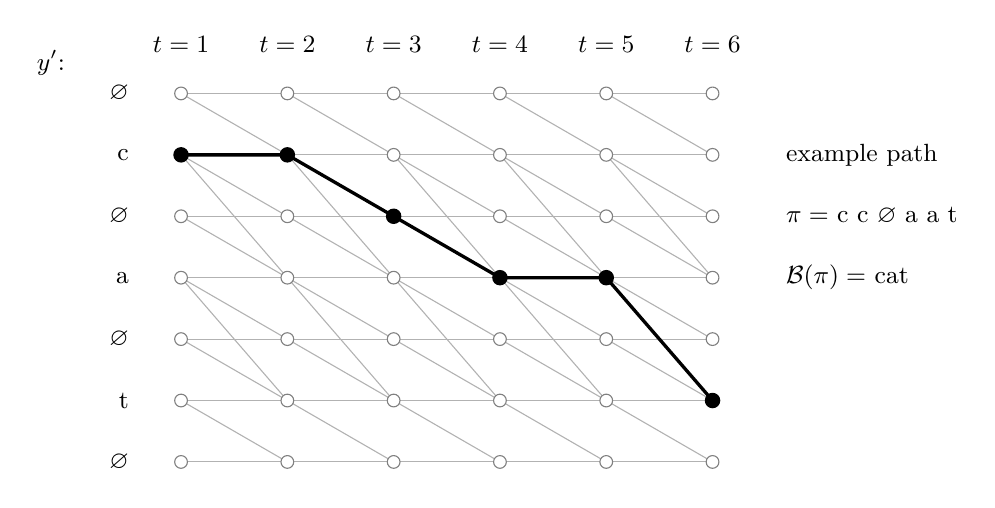
\begin{tikzpicture}[x={(1.35cm,0)},y={(0,-0.78cm)}]
\foreach \t in {1,...,5} {
  \foreach \s in {1,...,7} {\draw[gray!60] (\t,\s) -- (\t+1,\s);}
  \foreach \s in {1,...,6} {\draw[gray!60] (\t,\s) -- (\t+1,\s+1);}
  \draw[gray!60] (\t,2) -- (\t+1,4);
  \draw[gray!60] (\t,4) -- (\t+1,6);
}
\foreach \t in {1,...,6} {\foreach \s in {1,...,7} {\fill[white,draw=gray] (\t,\s) circle (2.3pt);}}
\foreach \s/\l in {1/$\varnothing$,2/c,3/$\varnothing$,4/a,5/$\varnothing$,6/t,7/$\varnothing$} {\node[font=\small,anchor=east] at (0.6,\s) {\l};}
\foreach \t in {1,...,6} {\node[font=\small,anchor=south] at (\t,0.5) {$t=\t$};}
\draw[very thick] (1,2) -- (2,2) -- (3,3) -- (4,4) -- (5,4) -- (6,6);
\foreach \t/\s in {1/2,2/2,3/3,4/4,5/4,6/6} {\fill (\t,\s) circle (2.8pt);}
\node[font=\small,anchor=west] at (6.6,2) {example path};
\node[font=\small,anchor=west] at (6.6,3) {$\pi=$ c c $\varnothing$ a a t};
\node[font=\small,anchor=west] at (6.6,4) {$\mathcal B(\pi)=$ cat};
\node[font=\small,anchor=east] at (0.0,0.5) {$y'$:};
\end{tikzpicture}
\caption{CTC lattice for the word ``cat'' with $T=6$ steps. The rows are the positions of the blank-augmented label $y'$; thin lines are the allowed transitions of Equation~\ref{eq:rec-alpha} (stay, advance, and skip over a blank between different letters). The thick path is one of the many paths that collapse to the word.}
\label{fig:rec-ctc}
\end{figure}

\paragraph{Receptive field.}
The region of the input that influences one feature is found with the recursion of Equation~\ref{eq:rec-rf}, in which $r$ is the receptive field and $j$ the distance in input pixels between adjacent features (the jump).
\begin{equation}
r_{\mathrm{out}}=r_{\mathrm{in}}+(k-1)\,j_{\mathrm{in}},\qquad j_{\mathrm{out}}=j_{\mathrm{in}}\,s.
\label{eq:rec-rf}
\end{equation}
Applied to the network (two convolutions, a pool, four convolutions, a pool, six convolutions) this gives 5, 6, 22, 24 and finally 72 pixels, so each column feature sees a $72\times72$ window, the full height of the line and about 18 time steps of context, before the recurrent layers add unbounded horizontal context.



\subsubsection{Evaluation metrics}

Accuracy is measured with the Levenshtein edit distance \cite{levenshtein1966}, the minimum number of insertions, deletions and substitutions that turn string $a$ into string $b$, computed by dynamic programming (Equation~\ref{eq:rec-lev}):
\begin{equation}
\begin{gathered}D[i][j]=\min\bigl(D[i-1][j]+1,\;D[i][j-1]+1,\;D[i-1][j-1]+\mathbb 1[a_i\ne b_j]\bigr),\\ D[i][0]=i,\ D[0][j]=j,\end{gathered}
\label{eq:rec-lev}
\end{equation}
with $d_{\mathrm{lev}}(a,b)=D[|a|][|b|]$.
For training and validation the character error rate is micro-averaged over all lines $n$ with prediction $\hat y_n$ and reference $y_n$ (Equation~\ref{eq:rec-cer}),
(equation as in the main text)
which is case-sensitive.
The end-to-end evaluation of Section~\ref{sec:results} instead averages per line the floored accuracy $\max(0,1-d_{\mathrm{lev}}(\hat y,y)/|y|)$ after converting both strings to lower case, which is slightly more lenient, so the two kinds of figure are not computed identically.
A word measure is implemented as the longest-common-subsequence (LCS) recall (Equation~\ref{eq:rec-wacc})
\begin{equation}
\mathrm{WordAcc}=\frac{\mathrm{LCS}(\text{reference words},\text{predicted words})}{\#\text{reference words}},
\label{eq:rec-wacc}
\end{equation}
which is an in-order recall and not $1-\mathrm{WER}$; a standard word error rate $\mathrm{WER}=d_{\mathrm{lev}}(\text{word sequences})/\#\text{reference words}$ was computed only once, when the public sets were re-evaluated.


\begin{figure}[h]
\centering
\begin{tikzpicture}[x=1cm,y=1cm]
\newcommand{\wcurve}[1]{\draw[#1] (0,0) .. controls (0.25,1.1) and (0.85,1.1) .. (0.7,0.45) .. controls (0.6,0.05) and (1.1,-0.05) .. (1.55,0.5);}
% column headings
\node[font=\small,align=center] at (1.0,3.25) {(a) raw crop};
\node[font=\small,align=center] at (4.2,3.25) {(b) core band};
\node[font=\small,align=center] at (7.4,3.25) {(c) skeleton};
\node[font=\small,align=center] at (10.6,3.25) {(d) re-inked};
% row A: thick, slanted
\begin{scope}[xshift=0.2cm,yshift=1.7cm,xslant=0.35]\wcurve{line width=5pt,gray!70,cap=round}\end{scope}
\begin{scope}[xshift=3.4cm,yshift=1.7cm,xslant=0.35]\wcurve{line width=5pt,gray!40,cap=round}\end{scope}
\draw[dashed] (3.3,1.55) -- (5.4,1.55) node[right,font=\scriptsize] {};
\draw[dashed] (3.3,2.35) -- (5.4,2.35);
\draw[<->] (5.2,1.55) -- (5.2,2.35); \node[font=\scriptsize,anchor=west] at (5.2,1.95) {$x_h$};
\begin{scope}[xshift=6.6cm,yshift=1.7cm,xslant=0.35]\wcurve{line width=0.8pt,black,cap=round}\end{scope}
\begin{scope}[xshift=9.8cm,yshift=1.7cm,xslant=0.35]\wcurve{line width=3pt,black,cap=round}\end{scope}
% row B: thin, upright
\begin{scope}[xshift=0.2cm,yshift=0.1cm]\wcurve{line width=1.8pt,gray!70,cap=round}\end{scope}
\begin{scope}[xshift=3.4cm,yshift=0.1cm]\wcurve{line width=1.8pt,gray!40,cap=round}\end{scope}
\draw[dashed] (3.3,-0.05) -- (5.4,-0.05);
\draw[dashed] (3.3,0.75) -- (5.4,0.75);
\draw[<->] (5.2,-0.05) -- (5.2,0.75); \node[font=\scriptsize,anchor=west] at (5.2,0.35) {$x_h$};
\begin{scope}[xshift=6.6cm,yshift=0.1cm]\wcurve{line width=0.8pt,black,cap=round}\end{scope}
\begin{scope}[xshift=9.8cm,yshift=0.1cm]\wcurve{line width=3pt,black,cap=round}\end{scope}
\node[font=\scriptsize,anchor=east] at (-0.2,2.0) {writer A};
\node[font=\scriptsize,anchor=east] at (-0.2,0.4) {writer B};
\draw[w2arr] (2.3,-0.9) -- (3.1,-0.9);
\end{tikzpicture}
\caption{Stroke normalisation of a schematic letter from two different writers. The raw strokes differ in thickness and slant (a); the core band gives the x-height $x_h$ (b); thinning reduces the stroke to a centre line (c); and the centre line is re-drawn with the width $w=\mathrm{round}(0.14\,x_h)$, identical for both writers (d). A real example is to be supplied as Figure~\ref{fig:wid-strokereal}.}
\label{fig:wid-strokenorm}
\end{figure}

\begin{itemize}
\item \emph{Skeletonisation.} The ink is thinned to a one-pixel centre line with the iterative algorithm of Zhang and Suen \cite{zhang1984}, which preserves the topology of the strokes. In each of two sub-iterations a pixel $p_1$ is deleted if the condition of Equation~\ref{eq:wid-zs} holds, namely
\begin{equation}
2\le B(p_1)\le6,\qquad A(p_1)=1,\qquad\text{and the product conditions of the sub-iteration,}
\label{eq:wid-zs}
\end{equation}
where $B(p_1)$ is the number of ink neighbours among the eight neighbours, $A(p_1)$ the number of transitions from background to ink around the ring of neighbours $P_2,\ldots,P_9$, and the product conditions are $P_2P_4P_6=0$ and $P_4P_6P_8=0$ (first sub-iteration) or $P_2P_4P_8=0$ and $P_2P_6P_8=0$ (second); the passes are repeated until no pixel changes.
\end{itemize}

\subsection{Appendix: further supporting material for Sections 3.3 to 3.5 (third condensation)}

This part of the appendix contains the staged-training diagram, the roles of the two writer classifiers, the optimisation paragraph with its equation, and the details of the text-versus-diagram clustering.

\begin{table}[h]
\centering
\fontsize{9.5}{11.5}\selectfont
\begin{tabularx}{\linewidth}{|p{3.3cm}|X|X|}
\hline
& \textbf{Ink-based classifier} & \textbf{Shape (stroke-normalised) classifier} \\
\hline
Input & Raw grey-scale line crop. & Line crop after stroke normalisation (constant pen width). \\
\hline
Used for & Real photographed pages in the classification mode. & Judging synthesised and G-code-rendered output, inside the best-of-$N$ search of Section~\ref{sec:synthesis}. \\
\hline
What was trained & All 966\,154 parameters, started from the weights of the text recogniser backbone. & Only the 13\,354 parameters of the head; the convolutional backbone is the frozen text-recogniser backbone. \\
\hline
\end{tabularx}
\caption{Roles of the two writer classifiers.}
\label{tab:wid-roles}
\end{table}

\paragraph{Optimisation.}
Both classifiers are trained with AdamW \cite{kingma2015,loshchilov2019}, which updates each parameter with a bias-corrected running mean $\hat m$ and running mean of squares $\hat v$ of the gradient and applies the weight decay separately from the gradient (Equation~\ref{eq:wid-adamw}):
\begin{equation}
\theta\leftarrow\theta-\eta\Bigl(\frac{\hat m}{\sqrt{\hat v}+\epsilon}+\lambda\theta\Bigr),\qquad\eta_t=\frac{\eta_0}{2}\Bigl(1+\cos\frac{\pi t}{T_{\max}}\Bigr),
\label{eq:wid-adamw}
\end{equation}
with weight decay $\lambda=10^{-4}$ and the cosine schedule of the learning rate $\eta_t$ over $T_{\max}$ epochs, which decreases smoothly from $\eta_0$ to zero.
Table~\ref{tab:wid-hyper} lists the settings.
The ink classifier is fully fine-tuned from the recogniser backbone, which has already learned stroke-shape features; the weights were compared and all 84 backbone tensors differ from the recogniser's.
For the shape classifier the frozen backbone (in inference mode) computes the 128-dimensional feature $f$ of every training image once, each line appearing four times (once unaugmented and three times with a different random augmentation), and only the head is trained on these 3\,680 stored vectors; all 84 backbone tensors of the stored shape model are bit-identical to those of the text recogniser.
Training only the head is fast and cannot overfit the thickness cue in the backbone, but it means that no augmentation is re-sampled between epochs.



\begin{figure}[h]
\centering
\begin{tikzpicture}[x=1cm,y=1cm]
\tikzset{sb/.style={w2box,text width=3.6cm,minimum height=1.4cm}}
\node[sb] (b) at (-5.4,0) {\textbf{1 Base}\\ own database lines, noisy labels\\ best val. loss 1.06};
\node[sb] (h) at (-0.6,0) {\textbf{2 Clean labels}\\ public line set, 6\,481 lines\\ val./test 93.87/91.60\,\%};
\node[sb] (n) at (4.5,1.2) {\textbf{3 Personal only (rejected)}\\ val./test 84.26/80.56\,\%\\ personal 90.2\,\%};
\node[sb] (j) at (4.5,-1.2) {\textbf{4 Joint, 80/20 sampler (deployed)}\\ val./test 94.03/91.82\,\%\\ personal 89.64\,\%};
\draw[w2arr] (b)--(h) node[midway,above,font=\scriptsize] {warm start};
\draw[w2arr] (h.east) -- ++(0.45,0) |- (n.west);
\draw[w2arr] (h.east) -- ++(0.45,0) |- (j.west);
\end{tikzpicture}
\caption{Staged training recipe of the text recogniser with the character accuracies (public validation and test sets, and personal validation; see Table~\ref{tab:rec-results} for the caveats).}
\label{fig:rec-stages}
\end{figure}

\paragraph{Text-versus-diagram clustering.}
A component with $\mathrm{mess}\ge0.5$, area above $0.8\wht^2$ and height above $1.2\wht$ becomes a candidate.
A candidate with a score below 0.85 is \emph{vetoed} (treated as text) when at least three text-sized neighbours stand in the same row band and the candidate is no taller than $1.9$ times the 75th percentile of their heights, which rescues large looped letters in headings.
Surviving candidates are clustered greedily by area into \texttt{MESS} blocks when their vertical gap is below $0.8\wht$ and their horizontal gap below $2\wht$, and each block receives a core box that ignores thin tails and labels.



\subsection{Appendix: further supporting material for Sections 3.3 and 3.4 (fourth condensation)}

This part of the appendix contains the full text and equations of the connected-component, skew, Gaussian-blur, batch-normalisation and staged-training passages that are summarised in Sections~\ref{sec:segmentation} and~\ref{sec:textrec}.

\subsubsection{Stage 7: connected components and the glyph-height scale}

A \emph{connected component} is a maximal set of ink pixels that touch each other.
Components are found with a run-length two-pass algorithm with union-find, a design that follows the classical sequential labelling idea \cite{rosenfeld1966} but works on runs instead of single pixels.
Each image row is first encoded as maximal runs $[s,e)$ of ink pixels.
For every pair of adjacent rows the runs are swept with two pointers, and run $i$ of the upper row and run $j$ of the lower row are merged when they touch; for 8-connectivity (diagonal neighbours count) the condition (Equation~\ref{eq:seg-adj}) is
\begin{equation}
s_i<e_j+1\ \ \wedge\ \ s_j<e_i+1,
\label{eq:seg-adj}
\end{equation}
and for 4-connectivity the $+1$ terms are dropped, where $s$ and $e$ are the start and end (exclusive) columns of the runs.
The pointer whose run ends first is advanced.
The merging uses a union-find structure with path halving \cite{tarjan1975}, roots are mapped to compact labels $1\ldots n$, and the labels are painted back run by run.
The cost is linear in the number of runs times an almost constant factor, which is far cheaper than a pixel-wise method for thin handwriting strokes.
For every component the area, bounding box and centroid are computed by sorting the labelled pixels by label.

The \emph{glyph height} $\wht$ is estimated from the components themselves, as given in Equation~\ref{eq:seg-ht}.
Heights of components with area at least 30 pixels and width below $12$ times the height (which excludes rules and long underlines) are collected; $h_{\mathrm{med}}$ is their median, and
\begin{equation}
\wht=\mathrm{median}\bigl\{h_c:\;0.3\,h_{\mathrm{med}}<h_c<3\,h_{\mathrm{med}}\bigr\},
\label{eq:seg-ht}
\end{equation}
where $h_c$ is the height of component $c$ (the default is 30 pixels if no component qualifies).
Because the cleaning stages change the component set, $\wht$ is computed three times: after the first binarisation (for the recovery stage), after faint filtering (for edge, column and rule removal), and finally on the cleaned set (for grouping and rendering).


\subsubsection{Stage 5: skew estimation and rotation}

If the text lines are tilted, row-based grouping and the recogniser both degrade.
The tilt of the page is estimated by the classical projection-profile principle: when the lines are horizontal, the row-sum profile of the ink has sharp peaks (line bodies) and deep troughs (gaps between lines), and any tilt smears them (Figure~\ref{fig:seg-skew}).
For a candidate angle $\theta$ the ink mask, reduced by a factor 4 (any ink in a $4\times4$ block), is rotated by nearest-neighbour sampling, the row profile $P_\theta(y)=\sum_xR_\theta(y,x)$ is formed, and the score is its variance (Equation~\ref{eq:seg-skew})
\begin{equation}
J(\theta)=\mathrm{Var}_y\bigl[P_\theta(y)\bigr],\qquad \theta^*=\arg\max_\theta J(\theta),
\label{eq:seg-skew}
\end{equation}
where $R_\theta$ is the rotated reduced mask and $\mathrm{Var}_y$ the variance over rows.
The search uses a coarse grid $\theta\in\{-r,-r+0.5,\ldots,r\}$ of 33 angles for $r=8^\circ$ followed by a fine grid $\theta^*\pm0.5^\circ$ in steps of $0.1^\circ$, so the angular resolution is $0.1^\circ$ and only 44 rotations of a mask of one sixteenth of the original area are needed.
Rotation about the image centre $(c_x,c_y)=((W-1)/2,(H-1)/2)$ uses inverse mapping with bilinear interpolation (nearest neighbour for masks):
\begin{equation}
\begin{pmatrix}x_s\\y_s\end{pmatrix}=\begin{pmatrix}\cos\theta&-\sin\theta\\ \sin\theta&\cos\theta\end{pmatrix}\begin{pmatrix}x-c_x\\y-c_y\end{pmatrix}+\begin{pmatrix}c_x\\c_y\end{pmatrix},
\label{eq:seg-rot}
\end{equation}
in which $(x,y)$ is an output pixel and $(x_s,y_s)$ the source position that is sampled; outside samples are filled with 255 for the colour page and 0 for masks.
The page is rotated only if $|\theta^*|\ge0.15^\circ$; stages 3 and 4 (grey conversion, correction, binarisation, speckle removal) are then recomputed on the rotated image, and a second residual pass with range $\pm3^\circ$ follows.


A single global angle is estimated, so page curl and keystone are not corrected; the objective was preferred to a Hough transform because ruled lines and diagrams dominate edge directions. A sign mismatch between rotation and scoring that doubled the skew in an early version was corrected.


\paragraph{Gaussian blur from three box blurs.}
A Gaussian blur with standard deviation $\sigma$ is approximated by three successive box means of equal radius $r$, because the repeated convolution of a uniform kernel converges to a Gaussian shape by the central-limit argument.
A single box of full width $w=2r+1$ has the variance $(w^2-1)/12$, and three independent passes add their variances to
\begin{equation}
\sigma_{\mathrm{real}}^2=\frac{w^2-1}{4},\qquad w=2r+1,\qquad r=\max\Bigl(1,\;\mathrm{round}\Bigl(\tfrac12\sqrt{\tfrac{4\sigma^2}{3}+1}\Bigr)\Bigr),
\label{eq:seg-gauss}
\end{equation}
where the radius $r$ is the one chosen by the implementation for a requested nominal scale $\sigma$.
An evaluation of Equation~\ref{eq:seg-gauss} shows that the box width produced by this rounding is approximately $\sqrt{4\sigma^2/3+1}+1$, so that $\sigma_{\mathrm{real}}\approx\sigma/\sqrt3\approx0.58\,\sigma$.
For example, a nominal scale $\sigma=60$ (the illumination blur for a page 1800 pixels wide) gives $r=35$, $w=71$ and $\sigma_{\mathrm{real}}=\sqrt{(71^2-1)/4}\approx35.5$, and a nominal scale of 9.5 gives $r=6$ and $\sigma_{\mathrm{real}}\approx6.5$.
The nominal $\sigma$ in this report is therefore a \emph{blur scale parameter} and not the realised standard deviation, and all constants of the block were tuned with the implementation as it stands.


\paragraph{Staged recipe.}
Training was carried out in four stages (Table~\ref{tab:rec-stages}, Figure~\ref{fig:rec-stages}), and each stage is motivated by a limitation that was found in the previous one.
\begin{enumerate}
\item \emph{Base stage.} The published recipe was reproduced on lines that were segmented from database pages by the student's own tools. The data turned out to be small and noisy because of the labelling defect and segmentation errors, and the best validation loss was 1.06.
\item \emph{Clean-label stage.} The network was warm-started from the base stage and trained on the public line-level IAM set, whose human-checked labels remove all segmentation and labelling noise.
\item \emph{Personal fine-tuning (rejected).} Fine-tuning on the personal lines alone raised the accuracy on the personal validation lines but reduced the accuracy on the general data by about ten points (catastrophic forgetting, Table~\ref{tab:rec-forget}); freezing the convolutional layers reduced the forgetting only slightly.
\item \emph{Joint stage (deployed).} Training continues from the clean-label stage on both data sets at once, with a weighted sampler: each public line receives the weight $w_T=(1-f)/n_T$ and each personal line $w_P=f/n_P$, where $n_T=6\,481$, $n_P\approx280$ and $f=0.20$, and $n_T$ indices are drawn per epoch with replacement with probability proportional to the weights (Equation~\ref{eq:rec-sampler}),
\begin{equation}
P(i)=\frac{w_i}{\sum_jw_j}.
\label{eq:rec-sampler}
\end{equation}
In expectation 20\,\% of every epoch ($\approx1\,296$ draws) is taken from the personal set, so that each personal line is seen about 4.6 times per epoch with fresh random augmentation, and 80\,\% from the public set. The checkpoint of the epoch with the largest $\min(\text{accuracy}_{\mathrm{public}},\text{accuracy}_{\mathrm{personal}})$ is kept, so that neither domain is sacrificed.
\end{enumerate}



A sweep over learning rate, LSTM width, depth, convolution width, dropout and optimiser (14 configurations of 50 epochs) was programmed, but no result file was kept, so the deployed architecture is the published one and not an optimum found by the student.
Training was done offline on a general-purpose computer; the training log of the joint stage was not kept, so epoch-by-epoch curves cannot be shown, and the stored joint checkpoint contains weights only.


\paragraph{Batch normalisation.}
Deep networks train poorly if the distribution of each layer's inputs keeps changing, so every convolution is followed by batch normalisation \cite{ioffe2015}.
During training, for each channel the mean $\mu_B$ and variance $\sigma_B^2$ are computed over the mini-batch and all spatial positions, and the output (Equation~\ref{eq:rec-bn}) is
\begin{equation}
\hat x=\frac{x-\mu_B}{\sqrt{\sigma_B^2+\varepsilon}},\qquad y=\gamma\hat x+\beta,\qquad\varepsilon=10^{-5},
\label{eq:rec-bn}
\end{equation}
where $\gamma$ and $\beta$ are learned scale and shift parameters of the channel.
Running averages of the mean and variance are kept during training, and at test time they replace $\mu_B$ and $\sigma_B^2$, which turns the layer into the fixed per-channel affine map $y=a\,x+b$ with
\begin{equation}
a=\frac{\gamma}{\sqrt{\sigma^2_{\mathrm{run}}+\varepsilon}},\qquad b=\beta-a\,\mu_{\mathrm{run}},
\label{eq:rec-bnfold}
\end{equation}
where $\mu_{\mathrm{run}}$ and $\sigma^2_{\mathrm{run}}$ are the running statistics; this is exactly the form that the inference implementation uses.


\subsection{Appendix: label generation for the database pages}

The labels of the database pages were produced by reading the printed prompt of each form and aligning its word list with the detected ink word runs by dynamic programming; the alignment cost for a run of measured width $a$ and an expected width $e$ is $c(a,e)=((a-e)/(e+1))^2$, with a penalty of 0.5 for the merging or splitting of words.

% Appendix material owned by writer 3 (extended tables, constants, derivations moved out of the main report)

\subsection{Style-profile schema and per-writer values}

This part of the appendix supports Section~\ref{sec:styleprofile}.
Table~\ref{tab:sty-schema} lists every key of a style-profile file with its meaning and an example value from the profile of writer 153, and Table~\ref{tab:sty-writers} lists the scalar values of all ten stored profiles.

{
\fontsize{9.5}{11.5}\selectfont
\setlength{\tabcolsep}{4pt}
\begin{longtable}{|p{3.2cm}|p{1.6cm}|p{6.6cm}|p{2.5cm}|}
\hline
\textbf{Key} & \textbf{Type} & \textbf{Meaning} & \textbf{Example (153)} \\
\hline
\endfirsthead
\hline
\textbf{Key} & \textbf{Type} & \textbf{Meaning} & \textbf{Example (153)} \\
\hline
\endhead
\hline
\endfoot
\texttt{authorId} & string & Writer identifier. & \texttt{"153"} \\
\hline
\texttt{slantDeg} & float & Median slant of the lines, forward lean positive (Equation~\ref{eq:sty-slant}). & 30.0 \\
\hline
\texttt{xHeightPx} & float & Median pixel x-height of the kept lines. & 33.0 \\
\hline
\texttt{strokeWidthXh} & float & Ink area divided by skeleton length, in x-heights. & 0.189 \\
\hline
\texttt{ascender}, \texttt{descender} & float & Typical reach of tall and descending lower-case glyphs, in x-heights (defaults 1.7 and $-0.6$ if no glyph qualifies). & 1.59, $-1.11$ \\
\hline
\texttt{wordSpaceXh} & float & Word gap measured on the real ink, in x-heights. & 1.59 \\
\hline
\texttt{connectedness} & float & Fraction of adjacent in-word letter pairs that the pen joins (Equation~\ref{eq:sty-conn}). & 0.97 \\
\hline
\texttt{letterAdvance} & dict & Median advance of each character, in x-heights (45 keys). & \texttt{T}: 1.438, \texttt{e}: 1.143 \\
\hline
\texttt{nLines} & int & Number of lines that survived the alignment-confidence cut. & 66 \\
\hline
\texttt{slantMeasRef}, \texttt{ascMeasRef}, \texttt{descMeasRef} & float & Slant (degrees) and ascender and descender reach of the real full lines, measured with the estimators later used on synthesised renders; input of the style calibration (Equation~\ref{eq:syn-cal}). & 30.0, 1.933, $-1.468$ \\
\hline
\texttt{inkFracRef}, \texttt{aspectRef}, \texttt{paperLevel}, \texttt{inkLevel}, \texttt{midFracRef} & float & Ink fraction, width-to-height ratio and grey statistics of the real lines; stored but ignored while the constant pen width is used for rendering. & 0.0620, 14.95, 246, 81, 0.038 \\
\hline
\texttt{glyphs} & dict & Variant library: for each character a list of at most 13 variant dictionaries (38 characters and 280 variants for writer 153). & see below \\
\hline
\texttt{idealGlyphs} & dict & Per-stroke median prototype of a letter (21 characters), with the keys \texttt{strokes}, \texttt{priorD}, \texttt{advance}, \texttt{lead}, \texttt{width}, \texttt{top}, \texttt{bot}, \texttt{entryY}, \texttt{exitY}, \texttt{nPool}. & --- \\
\hline
\texttt{idealMedoid} & dict & The real variant that is most typical of the writer (28 characters), same keys; this is the anchor used by the synthesiser. & --- \\
\hline
\texttt{legibilityLambda} & float & Legibility parameter $\lambda$ of Equations~\ref{eq:syn-global} and~\ref{eq:syn-swap}; added after the build. & 0.45 \\
\hline
\multicolumn{4}{|l|}{\textbf{Keys of one variant in \texttt{glyphs[c][i]}}} \\
\hline
\texttt{char} & string & The character. & \texttt{"e"} \\
\hline
\texttt{strokes} & list & Strokes, each a list of $[x,y]$ points in x-height units, baseline $y=0$, upright. & 2 and 38 points \\
\hline
\texttt{width}, \texttt{advance}, \texttt{lead} & float & Ink width, cell width and gap before the ink, in x-heights. & 0.878, 1.061, 0.0 \\
\hline
\texttt{top}, \texttt{bot} & float & Highest and lowest point. & 0.879, 0.061 \\
\hline
\texttt{entryX}, \texttt{entryY}, \texttt{exitX}, \texttt{exitY} & float & Entry and exit points of the pen for connectors. & $-0.204$, 0.333, 0.767, 0.182 \\
\hline
\texttt{connL}, \texttt{connR} & bool & The pen was joined to the left or right neighbour. & true, true \\
\hline
\texttt{priorD} & float & Cosine distance to the cross-writer letter prior (Equation~\ref{eq:sty-prior}). & 0.1127 \\
\hline
\texttt{denoised} & bool & Present and true if the variant is the denoised prototype. & --- \\
\hline
\caption{Keys of a style-profile file (JavaScript Object Notation).}
\label{tab:sty-schema}
\end{longtable}
}

\begin{table}[h]
\centering
\fontsize{9}{11}\selectfont
\setlength{\tabcolsep}{3pt}
\begin{tabular}{|l|r|r|r|r|r|r|r|r|r|r|r|}
\hline
\textbf{Writer} & \textbf{Lines} & \textbf{Slant ($^\circ$)} & \textbf{$x_h$ (px)} & \textbf{Stroke width} & \textbf{$A$} & \textbf{$D$} & \textbf{Gap} & \textbf{Conn.} & \textbf{$\lambda$} & \textbf{Chars} & \textbf{Var.} \\
\hline
150 & 61 & $-4.5$ & 46 & 0.097 & 1.58 & $-0.72$ & 1.33 & 0.347 & 0.90 & 40 & 295 \\
151 & 58 & 33.0 & 22 & 0.271 & 2.68 & $-1.09$ & 1.59 & 0.981 & 1.00 & 44 & 285 \\
152 & 59 & 19.5 & 46 & 0.103 & 1.48 & $-0.82$ & 1.47 & 0.735 & 0.45 & 37 & 271 \\
153 & 66 & 30.0 & 33 & 0.189 & 1.59 & $-1.11$ & 1.59 & 0.970 & 0.45 & 38 & 280 \\
384 & 54 & 4.5 & 43 & 0.107 & 1.95 & $-0.71$ & 1.37 & 0.472 & 0.30 & 36 & 256 \\
551 & 58 & 42.0 & 20 & 0.225 & 1.85 & $-0.68$ & 2.68 & 0.583 & 1.00 & 38 & 278 \\
552 & 47 & $-10.5$ & 31 & 0.149 & 1.64 & $-0.56$ & 1.53 & 0.621 & 0.00 & 38 & 279 \\
588 & 58 & 0.0 & 29 & 0.161 & 1.72 & $-0.67$ & 2.07 & 0.680 & 0.30 & 40 & 257 \\
dylan & 88 & $-7.5$ & 27 & 0.130 & 1.68 & $-0.61$ & 1.73 & 0.213 & 1.00 & 37 & 295 \\
yeukita & 138 & 0.0 & 27 & 0.145 & 1.46 & $-0.58$ & 0.92 & 0.432 & 0.15 & 56 & 376 \\
\hline
\end{tabular}
\caption{Scalar values of the ten stored style profiles: kept lines, slant, pixel x-height, stroke width (x-heights), ascender $A$ and descender $D$ and word gap (x-heights), connectedness, legibility parameter $\lambda$, number of characters and number of variants. Writers 150 to 588 are database writers, the last two are the personal writers.}
\label{tab:sty-writers}
\end{table}

\subsection{Constants of the synthesiser}

Table~\ref{tab:syn-const} lists the constants of Section~\ref{sec:synthesis} that are not given in the main text.

\begin{table}[h]
\centering
\fontsize{9.5}{11.5}\selectfont
\begin{tabularx}{\linewidth}{|p{5.2cm}|p{2.2cm}|X|}
\hline
\textbf{Constant} & \textbf{Value} & \textbf{Role} \\
\hline
Eligible variants per letter & 5 & Highest-ranked variants that can be drawn (Equation~\ref{eq:syn-pick}). \\
\hline
Clean and garbage prior distances & 0.12 and 0.55 & Limits of Equation~\ref{eq:syn-swap}. \\
\hline
Maximum prior distance of an anchor medoid & 0.30 & Otherwise the generic skeleton is used. \\
\hline
Connected-hand threshold for the cursive anchor & 0.5 & A value above 1 disables the cursive anchor (an earlier configuration used 2.0); lowering it to 0.3 lowered the evaluation score and was reverted. \\
\hline
Slant limit of anchor glyphs & $30^\circ$ / $22^\circ$ & Cursive / print skeleton. \\
\hline
Jitter share of anchor glyphs & 0.15 & Anchor glyphs wobble less. \\
\hline
Collision gap & 0.05 $x_{\mathrm{mm}}$ & Minimum clear space between consecutive ink boxes. \\
\hline
Output resampling and connector step & 0.35\,mm & Arc-length step of every pen-down polyline. \\
\hline
Rendering for the judges & 0.085 $x$, blur 0.30 & Constant pen width in x-heights and Gaussian blur as a fraction of the stroke width; 18 pixels per millimetre; padding $0.18\,x_{\mathrm{mm}}$. \\
\hline
Search stopping scores & 0.99 / 0.995 & Early stop of the candidate loop / no repair above this score. \\
\hline
Repair rounds and pins per round & 3 and 2 & Joint-aware repair pass. \\
\hline
Seed step between candidates & 977 & Candidate $k$ uses $\mathrm{base}+977k$. \\
\hline
Calibration probe & seed 17, $J=0$ & Sentence ``the quick brown fox jumps over lazy dogs and by half past eight it kept flying quietly''. \\
\hline
\end{tabularx}
\begin{tabularx}{\linewidth}{|X|c|c|}
\hline
\textbf{Perturbation (Equation~\ref{eq:syn-jit})} & \textbf{Standard deviation} & \textbf{At $J=0.5$, $x_{\mathrm{mm}}=4$\,mm} \\
\hline
Translation in $x$ / $y$ & $0.022J$ / $0.0132J$ x-heights & 0.044\,mm / 0.026\,mm \\
\hline
Rotation & $2.2^\circ J$ & $1.1^\circ$ \\
\hline
Scale in $x$ and $y$ (independent) & $0.05J$ & 2.5\,\% \\
\hline
Baseline drift (AR(1), clipped) & $0.05J\cdot0.35$ per step, $\pm0.25$ & $\pm0.25$ x-heights \\
\hline
Connector sag noise & $0.015\,x_{\mathrm{mm}}$ & 0.06\,mm \\
\hline
Word-gap factor & uniform 0.85 to 1.15 & --- \\
\hline
\end{tabularx}
\caption{Constants of the synthesiser and the jitter model.}
\label{tab:syn-const}
\end{table}

\subsection{G-code generator configuration}

Table~\ref{tab:gc-config} lists the machine configuration of the G-code generator of Section~\ref{sec:gcode}.
The motor, driver and transmission rows are assumptions made in the program comments; the calibrated steps per millimetre replace the derived values in the interpreter.

\begin{table}[h]
\centering
\fontsize{9.5}{11.5}\selectfont
\begin{tabularx}{\linewidth}{|p{4.2cm}|p{2.2cm}|X|}
\hline
\textbf{Field} & \textbf{Value} & \textbf{Meaning} \\
\hline
Full steps per revolution & 200 & Assumed 1.8$^\circ$ stepper motor. \\
\hline
Microstepping & 16 & Assumed driver setting. \\
\hline
Travel per revolution X, Y & 40.0\,mm & Assumed belt of 2\,mm pitch and a 20-tooth pulley. \\
\hline
Steps per millimetre (derived) & 80.000 & $200\cdot16/40$. \\
\hline
Work area & 0 to 200\,mm in X and Y & Limits of the clamp. \\
\hline
Origin and park position & (10, 180)\,mm & Top-left corner of the text block. \\
\hline
Draw feed & 900\,mm/min & Pen down (15\,mm/s). \\
\hline
Travel feed & 2400\,mm/min & Pen up (40\,mm/s); emitted once. \\
\hline
Acceleration & 400\,mm/s$^2$ & Used only by the time model. \\
\hline
Minimum segment & 0.12\,mm & Shorter moves are collapsed. \\
\hline
Pen pulse and settling time & 260\,ms and 90\,ms & Assumed time for a $90^\circ$ rotation and dwell after a toggle. \\
\hline
Pen codes & \texttt{M5}, \texttt{M3} & Pen up, pen down. \\
\hline
Pen state at power-on & up & Assumed. \\
\hline
\end{tabularx}
\caption{Configuration of the G-code generator.}
\label{tab:gc-config}
\end{table}

\subsection{Routes of the server application}

Table~\ref{tab:sys-endpoints} lists the routes of the server application of Section~\ref{sec:system}.

\begin{table}[h]
\centering
\fontsize{9}{11}\selectfont
\begin{tabularx}{\linewidth}{|c|p{4.0cm}|X|}
\hline
\textbf{Method} & \textbf{Path} & \textbf{Behaviour} \\
\hline
GET & \texttt{/\allowbreak api/\allowbreak authors} & List of the loaded writers with slant and connectedness. \\
\hline
POST & \texttt{/\allowbreak api/\allowbreak camera/\allowbreak capture} & Capture a still (from the open preview if there is one), store it, return an image identifier. \\
\hline
POST & \texttt{/\allowbreak api/\allowbreak camera/\allowbreak preview/\allowbreak start} and \texttt{/stop} & Open or release the camera for live framing. \\
\hline
GET & \texttt{/\allowbreak api/\allowbreak camera/\allowbreak preview/\allowbreak stream} & Live motion-JPEG stream; refused unless the preview is active. \\
\hline
GET & \texttt{/\allowbreak api/\allowbreak images/\allowbreak <id>} & Return a stored photograph. \\
\hline
POST & \texttt{/\allowbreak api/\allowbreak classify} & Photograph (file or identifier), optional expected text and writer; returns the recognised text, the character accuracy, the writer with its confidence, the per-writer mean probabilities and the number of lines; error 422 if no line is found. \\
\hline
POST & \texttt{/\allowbreak api/\allowbreak generate} & Text, writer and optional $N$ (default 20); returns the job identifier, G-code and preview addresses, line count, pen pulses, read-back text and accuracy and the synthesis time. \\
\hline
GET & \texttt{/\allowbreak api/\allowbreak gantry/\allowbreak status} & Connected, calibrated and the calibration; tries to connect as a side effect. \\
\hline
POST & \texttt{/\allowbreak api/\allowbreak gantry/\allowbreak calibrate} & Run the calibration (blocking). \\
\hline
POST & \texttt{/\allowbreak api/\allowbreak write/\allowbreak <job>} & Run the stored G-code on the gantry (blocking); reports not connected, not calibrated, aborted by an end-stop, or completed. \\
\hline
POST & \texttt{/\allowbreak api/\allowbreak gcode/\allowbreak upload} & Store an uploaded G-code file as a job and return its preview rendered from the file; nothing is sent to the gantry. \\
\hline
GET & \texttt{/\allowbreak api/\allowbreak gcode/\allowbreak <job>} and \texttt{/\allowbreak api/\allowbreak images/\allowbreak job\_<job>} & Raw G-code text and preview image of a job. \\
\hline
GET & \texttt{/\allowbreak api/\allowbreak model\_info} & Model architectures, sizes and stored accuracy figures. \\
\hline
GET & \texttt{/\allowbreak api/\allowbreak glyphs/\allowbreak <writer>} & Glyph-grid image of a writer's library (status 202 while it is being prepared). \\
\hline
GET & \texttt{/\allowbreak api/\allowbreak samples/\allowbreak <writer>} and \texttt{/\allowbreak api/\allowbreak samples/\allowbreak <writer>/\allowbreak <file>} & Sample crops of real lines with their transcriptions. \\
\hline
\end{tabularx}
\caption{Routes of the server application (18 routes; the optional access key is checked before every route).}
\label{tab:sys-endpoints}
\end{table}

\subsection{Supplementary figures and table for Sections 3.6 to 3.8}

This part of the appendix collects the figures and the cost table that support Sections~\ref{sec:styleprofile} to~\ref{sec:gcode}.
Figure~\ref{fig:sty-lattice} shows the forced-alignment lattice, Figure~\ref{fig:sty-dp} the Douglas--Peucker simplification, Figure~\ref{fig:sty-glyphs} a part of a stored library, Figure~\ref{fig:sty-stages} the placeholder for the builder stages on real lines, Figure~\ref{fig:syn-layout} the placement of glyphs, Figure~\ref{fig:syn-lines} two synthesised lines, Figure~\ref{fig:gc-frames} the coordinate frames and Table~\ref{tab:syn-cost} the cost of the search.

\begin{figure}[h]
\centering
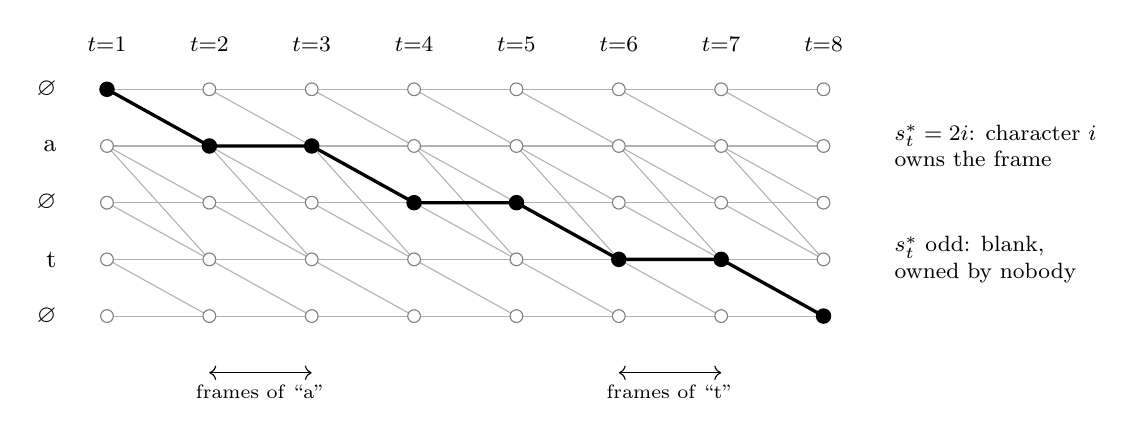
\begin{tikzpicture}[x={(1.3cm,0)},y={(0,-0.72cm)}]
\foreach \t in {1,...,7} {
  \foreach \s in {1,...,5} {\draw[gray!60] (\t,\s) -- (\t+1,\s);}
  \foreach \s in {1,...,4} {\draw[gray!60] (\t,\s) -- (\t+1,\s+1);}
  \draw[gray!60] (\t,2) -- (\t+1,4);
}
\foreach \t in {1,...,8} {\foreach \s in {1,...,5} {\fill[white,draw=gray] (\t,\s) circle (2.3pt);}}
\foreach \s/\l in {1/$\varnothing$,2/a,3/$\varnothing$,4/t,5/$\varnothing$} {\node[font=\small,anchor=east] at (0.6,\s) {\l};}
\foreach \t in {1,...,8} {\node[font=\footnotesize,anchor=south] at (\t,0.5) {$t{=}\t$};}
\draw[very thick] (1,1) -- (2,2) -- (3,2) -- (4,3) -- (5,3) -- (6,4) -- (7,4) -- (8,5);
\foreach \t/\s in {1/1,2/2,3/2,4/3,5/3,6/4,7/4,8/5} {\fill (\t,\s) circle (2.8pt);}
\draw[<->] (2,6.0) -- (3,6.0); \node[font=\scriptsize,anchor=north] at (2.5,6.05) {frames of ``a''};
\draw[<->] (6,6.0) -- (7,6.0); \node[font=\scriptsize,anchor=north] at (6.5,6.05) {frames of ``t''};
\node[font=\footnotesize,anchor=west,align=left] at (8.6,2) {$s^*_t=2i$: character $i$\\ owns the frame};
\node[font=\footnotesize,anchor=west,align=left] at (8.6,4) {$s^*_t$ odd: blank,\\ owned by nobody};
\end{tikzpicture}
\caption{Forced-alignment lattice for the transcript ``at'' with $T=8$ steps (cf.\ Figure~\ref{fig:rec-ctc}). The thick path is the Viterbi path of Equation~\ref{eq:sty-viterbi}; only the frames on the row of a letter belong to that letter, so the spans are narrow.}
\label{fig:sty-lattice}
\end{figure}

\begin{figure}[h]
\centering
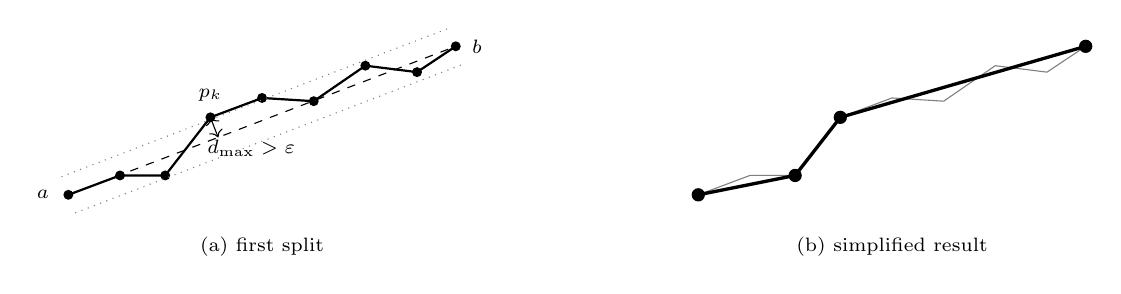
\begin{tikzpicture}[x=0.82cm,y=0.82cm]
\newcommand{\dppoly}[1]{\draw[#1] (0,0) -- (0.8,0.3) -- (1.5,0.3) -- (2.2,1.2) -- (3.0,1.5) -- (3.8,1.45) -- (4.6,2.0) -- (5.4,1.9) -- (6.0,2.3);}
\dppoly{thick}
\foreach \p in {(0,0),(0.8,0.3),(1.5,0.3),(2.2,1.2),(3.0,1.5),(3.8,1.45),(4.6,2.0),(5.4,1.9),(6.0,2.3)} {\fill \p circle (1.8pt);}
\draw[dashed] (0,0) -- (6.0,2.3);
\draw[gray,dotted] (-0.107,0.280) -- (5.893,2.580);
\draw[gray,dotted] (0.107,-0.280) -- (6.107,2.020);
\draw[<->] (2.2,1.2) -- (2.32,0.889);
\node[font=\scriptsize,anchor=west] at (2.0,0.72) {$d_{\max}>\varepsilon$};
\node[font=\scriptsize,anchor=east] at (-0.15,0) {$a$};
\node[font=\scriptsize,anchor=west] at (6.1,2.3) {$b$};
\node[font=\scriptsize] at (2.2,1.55) {$p_k$};
\node[font=\scriptsize,anchor=north] at (3.0,-0.5) {(a) first split};
\begin{scope}[xshift=8.0cm]
\dppoly{gray}
\draw[very thick] (0,0) -- (1.5,0.3) -- (2.2,1.2) -- (6.0,2.3);
\foreach \p in {(0,0),(1.5,0.3),(2.2,1.2),(6.0,2.3)} {\fill \p circle (2.4pt);}
\node[font=\scriptsize,anchor=north] at (3.0,-0.5) {(b) simplified result};
\end{scope}
\end{tikzpicture}
\caption{Douglas--Peucker simplification (schematic, tolerance exaggerated). (a) The vertex $p_k$ with the largest distance $d_{\max}$ from the chord $ab$ lies outside the tolerance band (dotted) and splits the chain. (b) After recursion on both halves four of the original nine vertices remain.}
\label{fig:sty-dp}
\end{figure}

\begin{figure}[h]
\centering

\includegraphics[width=\linewidth]{Figures/w3_glyphs153_ae.png}
\caption{Stored variants of the letters a, b, c, d and e of writer 153 (a strongly joined hand) in the glyph grid of the web interface; each row is one character with up to 12 variants. The short tails at the sides are remains of ligatures.}
\label{fig:sty-glyphs}
\end{figure}

\begin{figure}[h]
\centering
\figplaceholder{3.4cm}{One real line of a database writer and one personal line: grey crop, ink mask with rules removed and core band, Zhang--Suen skeleton, traced chains in colours with the territory cuts as vertical lines, and one extracted glyph in the normalised frame. Source: the functions of the profile builder applied to a crop of \texttt{Data/Datasets/IAMpages10} and one of \texttt{Software/CNN/NOGIT/dylan}.}
\caption{Stages of the style builder on real lines (placeholder).}
\label{fig:sty-stages}
\end{figure}

\begin{figure}[h]
\centering
\begin{tikzpicture}[x=1cm,y=1cm]
\newcommand{\hshape}[1]{\draw[#1] (0.1,0) -- (0.1,1.8); \draw[#1] (0.1,0.6) .. controls (0.3,1.0) and (0.7,1.0) .. (0.75,0.6) -- (0.75,0);}
\draw[gray] (-0.3,0) -- (4.3,0); \node[w3lab,anchor=east] at (-0.3,0) {baseline};
\draw[gray,dashed] (-0.3,1) -- (4.3,1); \node[w3lab,anchor=east] at (-0.3,1) {$y{=}1$};
\begin{scope}[xshift=0.2cm]\hshape{thick}\end{scope}
\begin{scope}[xshift=2.6cm,xslant=0.466]\hshape{thick}\end{scope}
\draw[w3arr] (1.2,0.9) -- (2.2,0.9);
\node[w3lab] at (1.7,1.15) {shear};
\draw[dotted] (2.7,0) -- (2.7,1.8);
\node[font=\scriptsize] at (2.0,-0.45) {(a) $X=\ell+x+y\tan\theta$};
\begin{scope}[xshift=6.3cm]
\draw[gray] (-0.3,0) -- (7.2,0);
\draw[fill=gray!10] (0,0) rectangle (2.3,1.4);
\draw[fill=gray!10] (2.3,0) rectangle (4.3,1.4);
\draw[thick] (0.5,0.1) rectangle (1.9,1.2);
\draw[thick] (2.55,0.1) rectangle (4.0,1.2);
\draw[<->] (0,-0.25) -- (2.3,-0.25); \node[w3lab,anchor=north] at (1.15,-0.25) {advance $a$};
\draw[<->] (0,1.6) -- (0.5,1.6); \node[w3lab,anchor=south] at (0.25,1.6) {$\ell$};
\draw[<->] (1.9,1.6) -- (2.55,1.6); \node[w3lab,anchor=south] at (2.3,1.6) {gap};
\draw[w3arr] (0,-0.9) -- (0.9,-0.9) node[midway,below,w3lab] {$P_x$};
\node[w3lab,anchor=west] at (4.4,0.7) {word gap $g\,x_{\mathrm{mm}}(0.85{+}0.3u)$};
\node[font=\scriptsize] at (3.2,-1.3) {(b) cells, ink boxes and guard};
\end{scope}
\end{tikzpicture}
\caption{Glyph placement. (a) A stored upright glyph is sheared by the writer's slant (Equation~\ref{eq:syn-place}). (b) Each glyph occupies a cell of its own advance $a$; the ink starts after the lead $\ell$, and the collision guard keeps a minimum clear gap between consecutive ink boxes.}
\label{fig:syn-layout}
\end{figure}

\begin{figure}[h]
\centering

\includegraphics[width=\linewidth]{Figures/w3_synth_150.png}\\[2pt]

\includegraphics[width=\linewidth]{Figures/w3_synth_153.png}
\caption{Synthesised line ``The gantry writes this sentence for the first time today'' for writer 150 (upper, printed hand; read back with three small errors) and writer 153 (lower, joined hand; read back as ``the garoby writes tttas senkence for tthe furst tuse today''), one seed and candidate each, rendered from the trajectory of an end-to-end run; the $N$ of that run was not recorded.}
\label{fig:syn-lines}
\end{figure}

\begin{figure}[h]
\centering
\begin{tikzpicture}[x=0.0225cm,y=0.0225cm]
\draw[fill=gray!8] (0,0) rectangle (204,262);
\draw[dashed] (5,5) rectangle (199,257);
\draw[thick] (5,5) rectangle (205,205);
\draw[thick,fill=gray!30] (15,40) rectangle (195,185);
\draw[w3arr] (5,5) -- (45,5) node[right,font=\scriptsize] {$X$};
\draw[w3arr] (5,5) -- (5,45) node[above,font=\scriptsize] {$Y$};
\fill (5,5) circle (3pt); \node[font=\scriptsize,anchor=north west] at (7,3) {machine $(0,0)$};
\fill (15,185) circle (3pt); \node[font=\scriptsize,anchor=south west] at (17,186) {$(X_{\mathrm{o}},Y_{\mathrm{o}})$};
\node[font=\scriptsize] at (105,110) {text block (illustrative)};
\draw[<->] (0,-18) -- (204,-18); \node[font=\scriptsize,anchor=north] at (102,-20) {204 mm switch-to-switch (X)};
\draw[<->] (-18,0) -- (-18,262); \node[font=\scriptsize,rotate=90,anchor=south] at (-20,131) {262 mm (Y)};
\node[font=\scriptsize,anchor=west,align=left] at (232,232) {dashed: driver usable area\\ $194\times252$ mm (5 mm edges)};
\node[font=\scriptsize,anchor=west,align=left] at (232,135) {solid: generator work area\\ $200\times200$ mm};
\end{tikzpicture}
\caption{Coordinate frames drawn to scale. The machine frame has its origin 5\,mm inside the minimum switches; the generator places the text block with its top-left corner at $(10,180)$\,mm inside a $200\times200$\,mm work area, and the driver clamps all targets to its calibrated usable area of $194\times252$\,mm. The extent of the text block is illustrative.}
\label{fig:gc-frames}
\end{figure}

\begin{table}[h]
\centering
\fontsize{9.5}{11.5}\selectfont
\begin{tabularx}{\linewidth}{|X|c|c|c|}
\hline
\textbf{Quantity (56-character sentence)} & \textbf{Writer 150} & \textbf{Writer 153} & \textbf{Writer 551} \\
\hline
Render size (pixels) & $3585\times225$ & $5508\times207$ & $7876\times277$ \\
\hline
Synthesis of one candidate (ms) & 11 & 13 & 16 \\
\hline
Rendering (ms) & 20 & 27 & 56 \\
\hline
Text recogniser (s) & 0.50 & 0.49 & 0.74 \\
\hline
Writer classifier incl. stroke normalisation (s) & 1.03 & 1.65 & 3.74 \\
\hline
Complete search, $N=14$, with repair attempts (s) & 23 & 37 & 137 \\
\hline
\end{tabularx}
\caption{Indicative cost of the search on the development laptop (single profiling run, unknown background load, jitter 0.5); times on the single-board computer were not recorded.}
\label{tab:syn-cost}
\end{table}

\subsection{Hardware information and timing measurements still to be supplied}

This part of the appendix supports Sections~\ref{sec:gantry} and~\ref{sec:system}.
Table~\ref{tab:gan-hw} lists the hardware items with the evidence in the project files, Figure~\ref{fig:gan-photo} is the placeholder for the photographs, and Table~\ref{tab:sys-timing} lists the stages of the timing chains.

\begin{table}[!htbp]
\centering
\fontsize{9.5}{11.5}\selectfont
\begin{tabularx}{\linewidth}{|p{2.6cm}|X|}
\hline
\textbf{Item} & \textbf{Evidence, and content to be supplied} \\
\hline
Computer & ODROID N2+ with 3.3\,V pins (Table~\ref{tab:gan-pins}). \\
\hline
Motors, drivers, transmission & Two motors with STEP/DIR driver modules; the program assumes 200 full steps per revolution, an A4988 at 1/16 microstepping and 40\,mm per revolution (2\,mm belt, 20-tooth pulley), and replaces the last by calibration. \textbf{[TO BE COMPLETED BY STUDENT: motor model, holding torque, rated current; driver model, current-limit setting, microstepping jumpers, minimum STEP pulse width; belt or screw type, pulley teeth, guides; whether any level shifter lies between the 3.3\,V pins and the drivers.]} \\
\hline
Travel & Measured switch-to-switch distances 204\,mm (X) and 262\,mm (Y). \textbf{[TO BE COMPLETED BY STUDENT: the calibrated steps per millimetre printed for both axes.]} \\
\hline
End-stops & Four switches, active-high at 3.3\,V, each with a pull-down of about 10\,k$\Omega$ (Figure~\ref{fig:gan-switch}). \textbf{[TO BE COMPLETED BY STUDENT: switch type and mounting.]} \\
\hline
Pen mechanism & One-direction gear motor whose cam toggles the pen every $90^\circ$, with a pen switch (high = up) (Section~\ref{sec:gan-pen}). \textbf{[TO BE COMPLETED BY STUDENT: how the motor is switched (transistor, flyback diode), supply voltage, pen model and holder, lift height.]} \\
\hline
Power supply (FU 4) & \textbf{[TO BE COMPLETED BY STUDENT: voltages and current ratings of the motor, computer and pen-motor supplies, grounding scheme, camera supply.]} The program comments state that the motors have no flyback diodes and share a ground return, which makes the switch inputs noisy (Section~\ref{sec:gan-stop}). \\
\hline
Camera (FU 1) & Generic USB video-class camera. \textbf{[TO BE COMPLETED BY STUDENT: model, resolution, mounting height, field of view, lamp.]} \\
\hline
\end{tabularx}
\caption{Hardware items: evidence in the project files and information still to be supplied.}
\label{tab:gan-hw}
\end{table}

\begin{figure}[!htbp]
\centering
\figplaceholder{2.4cm}{Photographs of the assembled gantry (axes, end-stops, pen holder with toggle motor, paper holder) and of the scanning rig with camera; CAD renderings and a wiring diagram with component values. To be supplied by the student.}
\caption{Photographs of the gantry and the scanning rig (placeholder).}
\label{fig:gan-photo}
\end{figure}

\begin{table}[!htbp]
\centering
\fontsize{9.5}{11.5}\selectfont
\begin{tabularx}{\linewidth}{|p{3.4cm}|X|}
\hline
\textbf{Stage} & \textbf{Known information and value to be supplied} \\
\hline
Capture & Framing by the user; five discarded frames without preview. \textbf{[TO BE COMPLETED BY STUDENT: time from pressing capture to the stored image.]} \\
\hline
Conditioning and segmentation & Whole page on the board. \textbf{[TO BE COMPLETED BY STUDENT: time per page on the board.]} \\
\hline
Recognition and writer classification & Two passes of about $4\times10^9$ multiply--accumulate operations per line. \textbf{[TO BE COMPLETED BY STUDENT: time per line on the board and total for the R4 test paragraph.]} \\
\hline
Synthesis & Returned in the server response; laptop values in Table~\ref{tab:syn-cost}. \textbf{[TO BE COMPLETED BY STUDENT: time on the board for the $N$ used in the demonstration.]} \\
\hline
G-code and preview & Milliseconds (not measured). \\
\hline
Gantry motion & Model 2.4 to 2.8\,s per character (Section~\ref{sec:gan-timing}). \textbf{[TO BE COMPLETED BY STUDENT: stopwatch time of a sentence of known length, from send to the final pen lift.]} \\
\hline
\end{tabularx}
\caption{Stages of the timing chains of the two modes and the measurements still missing.}
\label{tab:sys-timing}
\end{table}

\subsection{Design alternatives}

Tables~\ref{tab:sty-alt} and~\ref{tab:syn-alt} list the design alternatives of Sections~\ref{sec:styleprofile} and~\ref{sec:synthesis} with the reason for the chosen design.

\begin{table}[!htbp]
\centering
\fontsize{9.5}{11.5}\selectfont
\begin{tabularx}{\linewidth}{|p{3.0cm}|X|X|}
\hline
\textbf{Decision} & \textbf{Alternative} & \textbf{Reason for the chosen design} \\
\hline
Character boundaries & Fixed widths, projection minima, hand labelling. & Joined letters have no gaps and hand labelling of about 90 pages is impractical; the recogniser knows the text, so alignment is automatic. \\
\hline
Thin whole line, then cut & Thin each slice. & A slice edge creates a spurious spine stored as a bar. \\
\hline
Several variants per letter & One averaged letter. & Averaging blurs letters whose strokes are arranged differently; variants keep the natural variation, medoid and prototype remain options. \\
\hline
Prior as a filter & Import the median shape into every writer. & Importing would erase the writer; filtering keeps the shapes the writer's own. \\
\hline
Glyphs from scanned pages & Generator learned from on-line pen data. & No on-line data of the ten writers exist (47 to 138 usable lines each), and the pen path must be recovered from the image in any case (Section~\ref{sec:synthesis}). \\
\hline
\end{tabularx}
\caption{Design alternatives for the style extraction.}
\label{tab:sty-alt}
\end{table}

\begin{table}[!htbp]
\centering
\fontsize{9.5}{11.5}\selectfont
\begin{tabularx}{\linewidth}{|p{3.2cm}|X|}
\hline
\textbf{Alternative} & \textbf{Assessment} \\
\hline
Recurrent sequence generator with attention and mixture-density output \cite{graves2013} & Natural cursive, but needs on-line pen data (hundreds to thousands of lines per writer); only 47 to 138 scanned lines per writer exist. A from-scratch version trained on skeleton-derived strokes learned slant, roundness and connectedness but no legible letters. Rejected. \\
\hline
Adversarial or diffusion image generators \cite{kang2020,dai2024} & Low data need through pre-training, but the output is a raster: it needs vectorisation with the same thinning artefacts, size, slant and spacing cannot be controlled, and a trial took 35 to 45\,s (one line, laptop processor) to 2--3\,min against 3 to 8\,s for glyph synthesis. Rejected and parked. \\
\hline
Glyph assembly from one writer's sample \cite{haines2016} & Related approach; the present design adds the recogniser-aligned profile and the judge-driven search. \\
\hline
Glyph library with search (chosen) & Needs about nine pages per writer and no training; pen strokes are the native output; size, slant, joins and gap are explicit numbers; failures trace to one glyph; every glyph has a fallback. Weakness: cursive hands, whose joins are lost by cutting. \\
\hline
\end{tabularx}
\caption{Alternatives to the glyph-library synthesiser (timings are trial runs on a laptop without accelerator).}
\label{tab:syn-alt}
\end{table}

\subsection{Further figures and tables for Sections 3.8 to 3.10}

This part of the appendix supports Sections~\ref{sec:gcode} to~\ref{sec:system}.
Figure~\ref{fig:gc-excerpt} shows the start of a generated G-code program, Figure~\ref{fig:gc-vel} the velocity profiles of Equation~\ref{eq:gc-trap}, Table~\ref{tab:gan-pins} the pin assignment, Figure~\ref{fig:gan-switch} the switch input circuit and Table~\ref{tab:sys-modes} the chains of operations of the two online modes.

\begin{figure}[!htbp]
\begin{lstlisting}[basicstyle=\ttfamily\footnotesize,frame=none]
; Handwriting-Robot G-code -- author yeukita
; steps/mm  X=80.000  Y=80.000 (3200 microsteps/rev)
G21   ; millimetres
G90   ; absolute
G0 F2400                      <- travel feed, emitted once
G0 X10.059 Y179.271           <- travel to the first stroke
M3   ; pen DOWN (one 90deg pulse of the one-way gear motor)
G4 P0.350   ; wait for the 90deg rotation to finish
G1 F900                       <- draw feed
G1 X10.084 Y178.920           <- one line per vertex (0.35 mm apart)
...
M5   ; pen UP (one 90deg pulse of the one-way gear motor)
G4 P0.350
...                           <- next stroke; at the end: park, M2
\end{lstlisting}
\caption{Start of a generated program (test word of writer yeukita: 14 strokes, 239 draw moves, vertices 0.348\,mm apart on average); the arrows are annotations.}
\label{fig:gc-excerpt}
\end{figure}

\begin{figure}[!htbp]
\centering
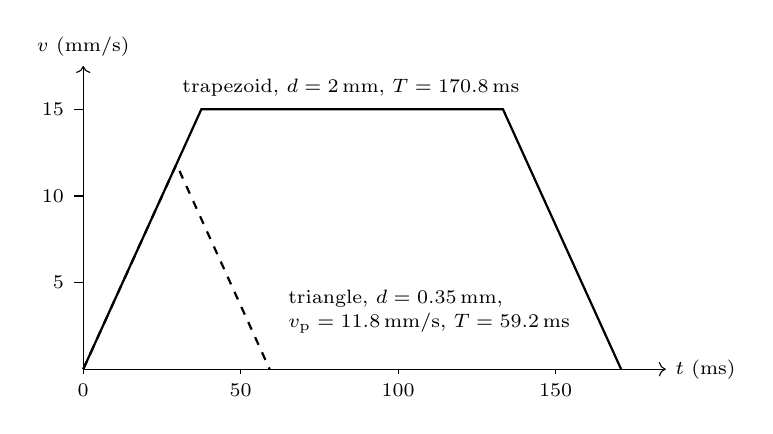
\begin{tikzpicture}[x=0.04cm,y=0.22cm]
\draw[->] (0,0) -- (185,0) node[right,font=\scriptsize] {$t$ (ms)};
\draw[->] (0,0) -- (0,17.5) node[above,font=\scriptsize] {$v$ (mm/s)};
\foreach \t in {0,50,100,150} {\draw (\t,0) -- (\t,-0.3) node[below,font=\scriptsize] {\t};}
\foreach \v in {5,10,15} {\draw (0,\v) -- (-3,\v) node[left,font=\scriptsize] {\v};}
\draw[thick] (0,0) -- (37.5,15) -- (133.3,15) -- (170.8,0);
\draw[thick,dashed] (0,0) -- (29.6,11.83) -- (59.2,0);
\node[font=\scriptsize,anchor=south] at (85,15.2) {trapezoid, $d=2$\,mm, $T=170.8$\,ms};
\node[font=\scriptsize,anchor=south west] at (62,3.0) {triangle, $d=0.35$\,mm,};
\node[font=\scriptsize,anchor=south west] at (62,1.5) {$v_{\mathrm p}=11.8$\,mm/s, $T=59.2$\,ms};
\end{tikzpicture}
\caption{Velocity profiles of Equation~\ref{eq:gc-trap} for $a=400$\,mm/s$^2$ and $v=15$\,mm/s: a 2\,mm move is trapezoidal (solid); the usual 0.35\,mm segment is triangular (dashed) and never reaches the cruise speed.}
\label{fig:gc-vel}
\end{figure}

\begin{table}[!htbp]
\centering
\fontsize{9.5}{11.5}\selectfont
\begin{tabularx}{\linewidth}{|X|c|c|c|c|}
\hline
\textbf{Function} & \textbf{Offset} & \textbf{Header pin} & \textbf{Direction} & \textbf{Initial level} \\
\hline
X motor DIR / STEP & 64 / 68 & 7 / 11 & output & high / low \\
\hline
Y motor DIR / STEP & 81 / 69 & 12 / 13 & output & high / low \\
\hline
X\_MIN / X\_MAX switch & 72 / 65 & 15 / 16 & input & --- \\
\hline
Y\_MIN / Y\_MAX switch & 66 / 67 & 18 / 22 & input & --- \\
\hline
Pen-position switch & 70 & 33 & input & --- \\
\hline
Pen motor drive & 71 & 35 & output & low \\
\hline
\end{tabularx}
\caption{Pin assignment of the gantry driver on \texttt{/dev/gpiochip0}, requested in one call; the header pin numbers are those of the program comments and were not checked against the board pinout.}
\label{tab:gan-pins}
\end{table}

\begin{figure}[!htbp]
\centering
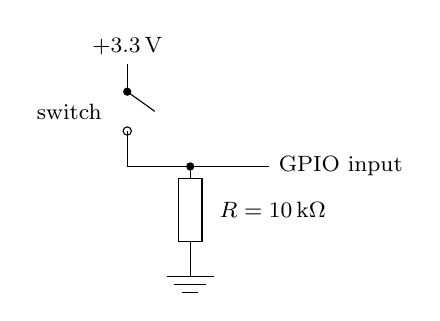
\begin{tikzpicture}[x=1cm,y=1cm,font=\footnotesize]
\draw (0,1.9) node[above] {$+3.3$\,V} -- (0,1.55);
\fill (0,1.55) circle (1.5pt); \draw (0,1.55) -- (0.35,1.3); \draw (0,1.05) circle (1.5pt); \draw (0,1.05) -- (0,0.6);
\node[anchor=east] at (-0.2,1.3) {switch};
\draw (0,0.6) -- (1.8,0.6) node[right] {GPIO input};
\fill (0.8,0.6) circle (1.5pt);
\draw (0.8,0.6) -- (0.8,0.45); \draw[fill=white] (0.65,0.45) rectangle (0.95,-0.35); \draw (0.8,-0.35) -- (0.8,-0.8);
\node[anchor=west] at (1.05,0.05) {$R=10$\,k$\Omega$};
\draw (0.5,-0.8) -- (1.1,-0.8); \draw (0.6,-0.9) -- (1.0,-0.9); \draw (0.7,-1.0) -- (0.9,-1.0);
\end{tikzpicture}
\caption{Switch input circuit as documented in the program comments; the closing current is $3.3\,\mathrm{V}/10\,\mathrm{k}\Omega=0.33$\,mA. The origin of the 3.3\,V (header pin) is inferred and \textbf{[TO BE CONFIRMED BY STUDENT]}.}
\label{fig:gan-switch}
\end{figure}

\begin{table}[!htbp]
\centering
\fontsize{9.5}{11.5}\selectfont
\begin{tabularx}{\linewidth}{|p{2.1cm}|p{2.1cm}|X|}
\hline
\textbf{Mode} & \textbf{Page} & \textbf{Chain of operations} \\
\hline
Classification & Read & Capture (live preview) or upload $\rightarrow$ conditioning and line segmentation $\rightarrow$ per line the text recogniser and the ink-based writer classifier $\rightarrow$ mean writer probabilities $\rightarrow$ text, writer, confidence and number of lines; with expected text and writer typed, also the character accuracy and a match mark. \\
\hline
Reproduction & Write & Calibrate once per session $\rightarrow$ text, writer and $N$ $\rightarrow$ best-of-$N$ synthesis $\rightarrow$ G-code, preview, read-back text and accuracy, pen pulses and synthesis time $\rightarrow$ ``send to gantry''. An uploaded G-code file uses the same preview and send path. \\
\hline
Training & (none) & Offline programs: segmentation of photographs, training of the networks and the profile builder (Section~\ref{sec:styleprofile}); the ten writers are pre-built files and the interface has no training function. \\
\hline
\end{tabularx}
\caption{Mapping of the proposal's modes to the web interface. A third page shows model architectures, sizes and stored accuracies, and for each writer sample crops and the glyph grid.}
\label{tab:sys-modes}
\end{table}

\subsection{Style calibration of the synthesiser}

Section~\ref{sec:syn-cal} describes the calibration; its three fixed-point iterations are, with ``ref'' the stored real-line value and ``got'' the value measured on the probe,
\begin{equation}
\Delta_\sigma\leftarrow\Delta_\sigma+\tan\theta_{\mathrm{ref}}-\tan\theta_{\mathrm{got}},\quad K_A\leftarrow\operatorname{clip}\Bigl(K_A\frac{A_{\mathrm{ref}}-1}{A_{\mathrm{got}}-1},0.5,1.6\Bigr),\quad K_D\leftarrow\operatorname{clip}\Bigl(K_D\frac{D_{\mathrm{ref}}}{D_{\mathrm{got}}},0.5,1.6\Bigr),
\label{eq:syn-cal}
\end{equation}
applied as $y\leftarrow1+(y-1)K_A$ for $y>1$ and $y\leftarrow yK_D$ for $y<0$ on the writer's own glyphs; $\Delta_\sigma$ is added to the shear coefficient of Equation~\ref{eq:syn-global}.

% Appendix material owned by writer 4 (extended QTP protocols)
\subsection{Extended qualification-test protocols}

This appendix gives the data sheets and definitions that support the qualification tests of Section~\ref{sec:res-qtp}.

\subsubsection{Metric definitions and detailed steps (qualification tests 1 and 5)}

Inter-rater agreement of the panel is quantified with Fleiss' kappa,
\begin{equation}
\label{eq:res-kappa}
\kappa=\frac{\bar P-\bar P_e}{1-\bar P_e},
\end{equation}
where $\bar P$ is the mean observed pairwise agreement and $\bar P_e$ the agreement expected by chance.
Each feature is $z$-scored, $z_{wf}=(v_{wf}-\mu_f)/\sigma_f$, using the mean and standard deviation over the ten real writers, and the stylistic correlation is
\begin{equation}
\label{eq:res-pearson}
\rho=\frac{\sum_{i}(a_i-\bar a)(b_i-\bar b)}{\sqrt{\sum_i(a_i-\bar a)^2}\sqrt{\sum_i(b_i-\bar b)^2}},
\end{equation}
where $a_i$ and $b_i$ are the real and synthesised $z$-scored entries pooled over 10 writers and 7 features (70 pairs); a per-writer value (7 pairs) and a nearest-centroid retrieval in $z$-space with its $10\times10$ confusion matrix are also computed.
For the overlay test (Figure~\ref{fig:res-overlay}) the skeleton point sets $A$ and $B$ are compared with
\begin{equation}
\label{eq:res-chamfer}
d_{\mathrm{ch}}(A,B)=\frac{1}{2}\left[\frac{1}{\lvert A\rvert}\sum_{a\in A}\min_{b\in B}\lVert a-b\rVert+\frac{1}{\lvert B\rvert}\sum_{b\in B}\min_{a\in A}\lVert a-b\rVert\right],
\end{equation}
\begin{equation}
\label{eq:res-mhd}
d_{\mathrm{MH}}(A,B)=\max\left[\frac{1}{\lvert A\rvert}\sum_{a\in A}\min_{b\in B}\lVert a-b\rVert,\;\frac{1}{\lvert B\rvert}\sum_{b\in B}\min_{a\in A}\lVert a-b\rVert\right],
\end{equation}
\begin{equation}
\label{eq:res-auc}
\mathrm{AUC}=\Pr\left[d_{\mathrm{matched}}<d_{\mathrm{mismatched}}\right]+\tfrac{1}{2}\Pr\left[d_{\mathrm{matched}}=d_{\mathrm{mismatched}}\right],
\end{equation}
where $\lVert\cdot\rVert$ is the Euclidean norm and distances are in units of the x-height $x_{\mathrm{h}}$.
Equation~\ref{eq:res-chamfer} is the mean of the two directed mean nearest-neighbour distances, Equation~\ref{eq:res-mhd} their maximum (less sensitive to outliers than the classical Hausdorff distance), and Equation~\ref{eq:res-auc} is 0.5 for a distance without writer information and 1.0 for perfect separation.
With 8 writers and 5 sentences there are 40 matched and $40\times9=360$ mismatched pairs.

\begin{figure}[h]
\centering
\begin{tikzpicture}
\node[resbox,text width=2.9cm] (real) at (0,0.9) {Genuine sentence image (held-out form, writer $w$)};
\node[resbox,text width=2.9cm] (syn) at (0,-0.9) {Synthesised image of the same text in style $w$ (or $w'$)};
\node[resbox,text width=2.7cm] (n1) at (4.1,0.9) {Crop to ink, scale to $x_{\mathrm{h}}$, align centroid};
\node[resbox,text width=2.7cm] (n2) at (4.1,-0.9) {Crop to ink, scale to $x_{\mathrm{h}}$, align centroid};
\node[resdark,text width=2.4cm] (d) at (8.0,0) {Skeleton point sets $A$, $B$: $d_{\mathrm{ch}}$, $d_{\mathrm{MH}}$};
\node[resbox,text width=2.3cm] (out) at (11.4,0) {Matched vs mismatched: AUC, rank-1};
\draw[resarr] (real)--(n1); \draw[resarr] (syn)--(n2);
\draw[resarr] (n1.east)--(d.north west); \draw[resarr] (n2.east)--(d.south west);
\draw[resarr] (d)--(out);
\end{tikzpicture}
\caption{Overlay test of qualification test 1: both images are normalised in the same way and matched writer pairs are compared with mismatched pairs.}
\label{fig:res-overlay}
\end{figure}

For qualification test 1 the steps are: (1) fix the held-out pages and freeze the system; (2) produce the 150 renderings (direct and G-code replay) on the ODROID N2+ and store writer, sentence, seed and text; (3) read every rendering with the base recogniser and evaluate Equation~\ref{eq:res-cacc} with the intervals; (4) run the panel with Table~\ref{tab:res-panel}, computing transcription accuracy and $\kappa$; (5) run the feature extractor and compute $\rho$ and the confusion matrix; (6) compute overlay distances, AUC and rank-1 retrieval and produce overlay figures for at least four sentences; (7) write a sentence on the gantry in a chosen style and count visibly matching characters (pass at 85\%).
Raters are 8 persons who are neither the student nor writers in the data set; the panel is blind and uses 30 synthesised lines (3 per writer) and 10 genuine control lines in random order, about 1350 scored characters per rater.

For qualification test 5 the absolute error and the measurement uncertainty are
\begin{equation}
\label{eq:res-r5}
e_i=\lVert\mathbf{p}_i-\mathbf{p}_i^{\mathrm{cmd}}\rVert,
\end{equation}
\begin{equation}
\label{eq:res-unc}
u=\sqrt{u_{\mathrm{scan}}^2+u_{\mathrm{ref}}^2+u_{\mathrm{id}}^2},
\end{equation}
where $\mathbf{p}_i$ is the measured and $\mathbf{p}_i^{\mathrm{cmd}}$ the commanded centre of cross $i$ (referenced to the machine origin 5~mm inside the minimum end-stops), $u_{\mathrm{scan}}$ the scanner scale error (from scanning the verified ruler), $u_{\mathrm{ref}}$ the registration of the sheet against the machine origin and $u_{\mathrm{id}}$ the error of locating a cross centre (half a pixel); the expanded uncertainty is $2u$.
The steps are: (1) calibrate and verify the direction pin on both axes and record the calibrated steps per millimetre; (2) fix the sheet against the stops, draw the grid, scan it with the ruler; (3) locate the cross centres with sub-pixel image analysis and compute $e_i$; (4) repeat 5 times and write the same word twice on one sheet for the overlay; (5) estimate $u$.
Repeatability is the radius of scatter of the 5 repeats of one cross about its centroid.

\subsubsection{Human legibility panel (qualification test 1)}

Table~\ref{tab:res-panel} is the worksheet that each of the 8 raters completes; it contains no information on whether a line is synthesised or genuine.

\begin{table}[h]
\centering
\fontsize{10}{12}\selectfont
\begin{tabularx}{\linewidth}{|l|X|l|l|}
\hline
\textbf{Line no.} & \textbf{Transcription written by the rater (without hint of the content)} & \textbf{Illegible characters (positions)} & \textbf{Confidence (1--5)} \\
\hline
1 & & & \\
\hline
2 & & & \\
\hline
$\vdots$ & & & \\
\hline
40 & & & \\
\hline
\end{tabularx}
\caption{Worksheet for the blind human panel: 30 synthesised lines and 10 genuine control lines in random order.}
\label{tab:res-panel}
\end{table}

\subsubsection{Style-feature definitions (qualification test 1)}

The features of Table~\ref{tab:res-features} are computed by one deterministic extractor with identical thresholds on every image, after cropping to the ink and binarising with the same rule.

\begin{table}[h]
\centering
\fontsize{10}{12}\selectfont
\begin{tabularx}{\linewidth}{|>{\raggedright\arraybackslash}p{3.3cm}|X|}
\hline
\textbf{Feature} & \textbf{Definition} \\
\hline
Slant & Shear angle (degrees) that maximises the variance of the column ink projection of the line. \\
\hline
Stroke width & Median stroke width from the distance transform at the skeleton, divided by $x_{\mathrm{h}}$. \\
\hline
Ink density & Fraction of ink pixels inside the core band between the baseline and the x-height line. \\
\hline
Word gap & Median horizontal gap between words (gaps larger than $0.5\,x_{\mathrm{h}}$) divided by $x_{\mathrm{h}}$. \\
\hline
Connectedness & Number of connected ink components divided by the number of characters of the text. \\
\hline
Character width & Line width divided by the number of characters, divided by $x_{\mathrm{h}}$. \\
\hline
Ascender/descender ratio & (Height of the ascender zone plus depth of the descender zone) divided by $x_{\mathrm{h}}$. \\
\hline
\end{tabularx}
\caption{Hand-crafted style features for the correlation and retrieval of qualification test 1 (definitions to be implemented by the student exactly as listed).}
\label{tab:res-features}
\end{table}

\subsubsection{Hardware overlay measurement sheet (qualification test 5)}

Table~\ref{tab:res-sheet} is the sheet on which the measurements of the grid test are recorded for each repetition.

\begin{table}[h]
\centering
\fontsize{10}{12}\selectfont
\begin{tabularx}{\linewidth}{|l|l|l|l|l|l|X|}
\hline
\textbf{Repeat} & \textbf{Cross} & \textbf{$x^{\mathrm{cmd}}$ (mm)} & \textbf{$y^{\mathrm{cmd}}$ (mm)} & \textbf{$x$ meas. (mm)} & \textbf{$y$ meas. (mm)} & \textbf{$e_i$ (mm)} \\
\hline
1 & 1 & & & & & \\
\hline
1 & 2 & & & & & \\
\hline
$\vdots$ & & & & & & \\
\hline
\end{tabularx}
\caption{Data sheet for the absolute positional error of qualification test 5; one row per cross and repetition, together with the scanner scale check and the registration check.}
\label{tab:res-sheet}
\end{table}



\end{document}

%% End of File.
